%!TEX program = xelatex
% Encoding: UTF8

% LaTeX source for ``Think Python: How to Think Like a Computer Scientist''
% Copyright (c)  2015  Allen B. Downey.Glossary

% License: Creative Commons Attribution-NonCommercial 3.0 Unported License.
% http://creativecommons.org/licenses/by-nc/3.0/
%

%\documentclass[10pt,b5paper]{book}
%\documentclass[10pt]{book}
\documentclass[11pt,b5paper]{ctexbook} % support chinese

\usepackage[width=5.5in,height=8.5in,
  hmarginratio=3:2,vmarginratio=1:1]{geometry}

% for some of these packages, you might have to install
% texlive-latex-extra (in Ubuntu)

\usepackage[T1]{fontenc}
\usepackage{textcomp}
\usepackage{mathpazo}
\usepackage{url}
\usepackage{fancyhdr}
\usepackage{graphicx}
\usepackage{amsmath}
\usepackage{amsthm}
%\usepackage{amssymb}
\usepackage{exercise}                        % texlive-latex-extra
\usepackage{makeidx}
\usepackage{setspace}
\usepackage{hevea}
\usepackage{upquote}
\usepackage{appendix}
\usepackage[bookmarks]{hyperref}

\usepackage{xcolor}
\definecolor{mygreen}{rgb}{0,0.6,0}
\definecolor{mygray}{rgb}{0.5,0.5,0.5}
\definecolor{codeback}{rgb}{0.93,0.89,0.86}

\newfontfamily\CodeFont{Consolas}
% \newfontfamily\CodeFont{Monaco}


\usepackage{listings}
\lstset{ %
  backgroundcolor=\color{codeback},    % choose the background color; you must add \usepackage{color} or \usepackage{xcolor}
  basicstyle=\linespread{0.95}\small\CodeFont,   % the size of the fonts that are used for the code
  breakatwhitespace=false,           % sets if automatic breaks should only happen at whitespace
  breaklines=true,                   % sets automatic line breaking
  captionpos=bl,                     % sets the caption-position to bottom
  commentstyle=\color{mygreen},      % comment style
  deletekeywords={...},              % if you want to delete keywords from the given language
  escapeinside={\%*}{*)},            % if you want to add LaTeX within your code
  extendedchars=true,                % lets you use non-ASCII characters; for 8-bits encodings only, does not work with UTF-8
  frame=single,                      % adds a frame around the code
  frameround=tttt,
  keepspaces=true,                   % keeps spaces in text, useful for keeping indentation of code (possibly needs columns=flexible)
  keywordstyle=\color{blue},         % keyword style
  language=Python,                   % the language of the code
  morekeywords={*,...},              % if you want to add more keywords to the set
  numbers=none,                      % where to put the line-numbers; possible values are (none, left, right)
  numbersep=5pt,                     % how far the line-numbers are from the code
  numberstyle=\tiny\CodeFont\color{mygray},   % the style that is used for the line-numbers
  rulecolor=\color{mygray},          % if not set, the frame-color may be changed on line-breaks within not-black text (e.g. comments (green here))
  showspaces=false,                  % show spaces everywhere adding particular underscores; it overrides 'showstringspaces'
  showstringspaces=true,             % underline spaces within strings only
  showtabs=true,                     % show tabs within strings adding particular underscores
  stepnumber=1,                      % the step between two line-numbers. If it's 1, each line will be numbered
  stringstyle=\color{orange},        % string literal style
  tabsize=2,                         % sets default tabsize to 2 spaces
  %title=myPython.py                 % show the filename of files included with \lstinputlisting; also try caption instead of title
  xleftmargin = 1em,
  xrightmargin = 1em,
  aboveskip = 1 em
}



\title{Think Python}
\author{Allen B. Downey}
\newcommand{\thetitle}{Think Python: How to Think Like a Computer Scientist}
\newcommand{\theversion}{2nd Edition, Version 2.2.14}
\newcommand{\thedate}{}

% these styles get translated in CSS for the HTML version
\newstyle{a:link}{color:black;}
\newstyle{p+p}{margin-top:1em;margin-bottom:1em}
\newstyle{img}{border:0px}

% change the arrows
\setlinkstext
  {\imgsrc[ALT="Previous"]{back.png}}
  {\imgsrc[ALT="Up"]{up.png}}
  {\imgsrc[ALT="Next"]{next.png}}

\makeindex

\newif\ifplastex
\plastexfalse

\begin{document}

\frontmatter

% PLASTEX ONLY
\ifplastex
    \usepackage{localdef}
    \maketitle

\newcount\anchorcnt
\newcommand*{\Anchor}[1]{%
  \@bsphack%
    \Hy@GlobalStepCount\anchorcnt%
    \edef\@currentHref{anchor.\the\anchorcnt}%
    \Hy@raisedlink{\hyper@anchorstart{\@currentHref}\hyper@anchorend}%
    \M@gettitle{}\label{#1}%
    \@esphack%
}


\else
% skip the following for plastex

\newtheorem{exercise}{Exercise}[chapter]

% LATEXONLY

% \setlength{\parindent}{2em}
\usepackage[width=5.5in,height=8.5in,
  hmarginratio=3:2,vmarginratio=1:1]{geometry}
\setCJKmainfont[BoldFont=SimHei, ItalicFont=STKaiti]{SimSun}
\setCJKmonofont[Scale=0.9]{Consolas}
\setCJKfamilyfont{song}[BoldFont=SimSun]{SimSun}
\setCJKfamilyfont{sf}[BoldFont=SimSun]{SimSun}
\XeTeXlinebreaklocale "zh"
\XeTeXlinebreakskip = 0pt plus 1pt

\usepackage{xeCJK}
\usepackage{indentfirst}

\usepackage[T1]{fontenc}
\usepackage{textcomp}
\usepackage{mathpazo}
\usepackage{url}
\usepackage{fancyhdr}
\usepackage{graphicx}
\usepackage{amsmath}
\usepackage{amsthm}
%\usepackage{amssymb}
\usepackage{exercise}                        % texlive-latex-extra
\usepackage{makeidx}
\usepackage{setspace}
\usepackage{hevea}                           
\usepackage{upquote}
\usepackage{appendix}
\usepackage{hyperref}

\sloppy
%\setlength{\topmargin}{-0.375in}
%\setlength{\oddsidemargin}{0.0in}
%\setlength{\evensidemargin}{0.0in}

% Uncomment these to center on 8.5 x 11
%\setlength{\topmargin}{0.625in}
%\setlength{\oddsidemargin}{0.875in}
%\setlength{\evensidemargin}{0.875in}

%\setlength{\textheight}{7.2in}

\setlength{\headsep}{3ex}
\setlength{\parskip}{1.7ex plus 0.5ex minus 0.5ex}
\setcounter{chapter}{-1}

\renewcommand{\baselinestretch}{1.02}

% see LaTeX Companion page 62
\setlength{\topsep}{-0.0\parskip}
\setlength{\partopsep}{-0.5\parskip}
\setlength{\itemindent}{0.0in}
\setlength{\listparindent}{0.0in}

% see LaTeX Companion page 26
% these are copied from /usr/local/teTeX/share/texmf/tex/latex/base/book.cls
% all I changed is afterskip

\makeatletter

\renewcommand{\section}{\@startsection 
    {section} {1} {0mm}%
    {-3.5ex \@plus -1ex \@minus -.2ex}%
    {0.7ex \@plus.2ex}%
    {\normalfont\Large\bfseries}}
\renewcommand\subsection{\@startsection {subsection}{2}{0mm}%
    {-3.25ex\@plus -1ex \@minus -.2ex}%
    {0.3ex \@plus .2ex}%
    {\normalfont\large\bfseries}}
\renewcommand\subsubsection{\@startsection {subsubsection}{3}{0mm}%
    {-3.25ex\@plus -1ex \@minus -.2ex}%
    {0.3ex \@plus .2ex}%
    {\normalfont\normalsize\bfseries}}

% The following line adds a little extra space to the column
% in which the Section numbers appear in the table of contents
\renewcommand{\l@section}{\@dottedtocline{1}{1.5em}{3.0em}}
\setcounter{tocdepth}{1}

\makeatother

\newcommand{\beforefig}{\vspace{1.3\parskip}}
\newcommand{\afterfig}{\vspace{-0.2\parskip}}

\newcommand{\beforeverb}{\vspace{0.6\parskip}}
\newcommand{\afterverb}{\vspace{0.6\parskip}}

\newcommand{\adjustpage}[1]{\enlargethispage{#1\baselineskip}}


% Note: the following command seems to cause problems for Acroreader
% on Windows, so for now I am overriding it.
%\newcommand{\clearemptydoublepage}{
%            \newpage{\pagestyle{empty}\cleardoublepage}}
\newcommand{\clearemptydoublepage}{\cleardoublepage}

%\newcommand{\blankpage}{\pagestyle{empty}\vspace*{1in}\newpage}
\newcommand{\blankpage}{\vspace*{1in}\newpage}

% HEADERS

\renewcommand{\chaptermark}[1]{\markboth{#1}{}}
\renewcommand{\sectionmark}[1]{\markright{\thesection\ #1}{}}

\lhead[\fancyplain{}{\bfseries\thepage}]%
      {\fancyplain{}{\bfseries\rightmark}}
\rhead[\fancyplain{}{\bfseries\leftmark}]%
      {\fancyplain{}{\bfseries\thepage}}
\cfoot{}

\pagestyle{fancyplain}


% turn off the rule under the header
%\setlength{\headrulewidth}{0pt}

% the following is a brute-force way to prevent the headers
% from getting transformed into all-caps
\renewcommand\MakeUppercase{}

% Exercise environment
\newtheoremstyle{myex}% name
     {9pt}%      Space above
     {9pt}%      Space below
     {}%         Body font
     {}%         Indent amount (empty = no indent, \parindent = para indent)
     {\bfseries}% Thm head font
     {}%        Punctuation after thm head
     {0.5em}%     Space after thm head: " " = normal interword space;
           %       \newline = linebreak
     {}%         Thm head spec (can be left empty, meaning `normal')

\theoremstyle{myex}


\begin{latexonly}

\renewcommand{\blankpage}{\thispagestyle{empty} \quad \newpage}

%\blankpage
%\blankpage

% TITLE PAGES FOR LATEX VERSION

%-half title--------------------------------------------------
\thispagestyle{empty}

\begin{flushright}
\vspace*{2.0in}

\begin{spacing}{3}
{\huge Think Python}\\
{\Large How to Think Like a Computer Scientist}
\end{spacing}

\vspace{0.25in}

\theversion

\thedate

\vfill

\end{flushright}

%--verso------------------------------------------------------

\blankpage
\blankpage
%\clearemptydoublepage
%\pagebreak
%\thispagestyle{empty}
%\vspace*{6in}

%--title page--------------------------------------------------
\pagebreak
\thispagestyle{empty}

\begin{flushright}
\vspace*{2.0in}

\begin{spacing}{3}
{\huge Think Python}\\
{\Large How to Think Like a Computer Scientist}
\end{spacing}

\vspace{0.25in}

\theversion

\thedate

\vspace{1in}


{\Large
Allen Downey\\
}


\vspace{0.5in}

{\Large Green Tea Press}

{\small Needham, Massachusetts}

% \includegraphics[width=1in]{../source/figs/logo1.pdf}
\vfill

\end{flushright}


%--copyright--------------------------------------------------
\pagebreak
\thispagestyle{empty}

{\small
Copyright \copyright ~2015 Allen Downey.


\vspace{0.2in}

\begin{flushleft}
Green Tea Press       \\
9 Washburn Ave        \\
Needham MA 02492
\end{flushleft}

Permission is granted to copy, distribute, and/or modify this document
under the terms of the Creative Commons Attribution-NonCommercial 3.0 Unported
License, which is available at \url{http://creativecommons.org/licenses/by-nc/3.0/}.

The original form of this book is \LaTeX\ source code.  Compiling this
\LaTeX\ source has the effect of generating a device-independent
representation of a textbook, which can be converted to other formats
and printed.

The \LaTeX\ source for this book is available from
\url{http://www.thinkpython2.com}

\vspace{0.2in}

} % end small

\end{latexonly}


% HTMLONLY

\begin{htmlonly}

% TITLE PAGE FOR HTML VERSION

{\Large \thetitle}

{\large Allen B. Downey}

\theversion

\thedate

\setcounter{chapter}{-1}

\end{htmlonly}

\fi
% END OF THE PART WE SKIP FOR PLASTEX


\chapter{Preface  |  前言}

\section*{The strange history of this book  |  本书与众不同的历史}

In January 1999 I was preparing to teach an introductory programming
class in Java.  I had taught it three times and I was getting
frustrated.  The failure rate in the class was too high and, even for
students who succeeded, the overall level of achievement was too low.

1999年1月,我正准备使用Java教一门编程入门课程。我之前已经开了三次课, 但是却感到越来越沮丧。课程的不及格率太高,即使对于及格的学生,他们整体的收获也太低。

One of the problems I saw was the books.
They were too big, with too much unnecessary detail about Java, and
not enough high-level guidance about how to program.  And they all
suffered from the trap door effect: they would start out easy,
proceed gradually, and then somewhere around Chapter 5 the bottom would
fall out.  The students would get too much new material, too fast,
and I would spend the rest of the semester picking up the pieces.

我看到的问题之一是教材。

它们都太厚重了,写了太多关于Java的不必要细节,却缺乏如何编程的上层指导 (high-level guidance)。这些教材都陷入了陷阱门效应(trap door effect):开始的时候简单,逐渐深入,然后大概到了第五章左右,基础差的学生就跟不上了。 学生们看的材料太多,进展太快,最后,我在接下来的学期里都是在收拾残局(pick up the pieces)。

Two weeks before the first day of classes, I decided to write my
own book.  My goals were:

\begin{itemize}

\item Keep it short.  It is better for students to read 10 pages
than not read 50 pages.

\item Be careful with vocabulary.  I tried to minimize jargon
and define each term at first use.

\item Build gradually. To avoid trap doors, I took the most difficult
topics and split them into a series of small steps.

\item Focus on programming, not the programming language.  I included
the minimum useful subset of Java and left out the rest.

\end{itemize}

所以,在开始上课前两周,我决定自己写一本书。我的目标是:

\begin{itemize}

\item 尽量简短。让学生们读10页,胜过让他们读50页。

\item 谨慎使用术语。我会尽量少用术语,而且第一次使用时,会给出定义。

\item 循序渐进。为了避免陷阱门,我将最难的主题拆分成了很多个小节。

\item 聚焦于编程,而不是编程语言。我只涵盖了Java最小可用子集,剔除了其余的部分。

\end{itemize}

I needed a title, so on a whim I chose {\em How to Think Like
a Computer Scientist}.

我需要一个书名,所以一时兴起,我选择了\emph{《如何像计算机科学家一样思考》}。

My first version was rough, but it worked.  Students did the reading,
and they understood enough that I could spend class time on the hard
topics, the interesting topics and (most important) letting the
students practice.

这本书的第一版很粗糙,但是却起了作用。学生们读了它之后,对书中内容理解的很好, 因此我才可以在课堂上讲授那些困难、有趣的主题,并让学生们动手实践(这点最重要)。

I released the book under the GNU Free Documentation License,
which allows users to copy, modify, and distribute the book.

我将此书以GNU自有文档许可的形式发布,允许用户拷贝、修改和传播此书。
\index{GNU Free Documentation License} \index{Free Documentation License, GNU}

What happened next is the cool part.  Jeff Elkner, a high school
teacher in Virginia, adopted my book and translated it into
Python.  He sent me a copy of his translation, and I had the
unusual experience of learning Python by reading my own book.
As Green Tea Press, I published the first Python version in 2001.

有趣的是接下来发生的事。弗吉尼亚一所高中的教师Jeff Elkne采用了我的教材, 并改为使用Python语言。他将修改过的书发给了我一份,就这样,我读着自己的书学会了 Python。2001年,通过Green Tea Press,我出版了本书的第一个Python版本。
\index{Elkner, Jeff}

In 2003 I started teaching at Olin College and I got to teach
Python for the first time.  The contrast with Java was striking.
Students struggled less, learned more, worked on more interesting
projects, and generally had a lot more fun.

2003年,我开始在Olin College教书,并且第一次教授Python语言。 与Java教学的对比很明显。学生们遇到的困难更少,学到的更多,开发了更有趣的工程, 并且大部分人都学的更开心。
\index{Olin College}

Since then I've continued to develop the book,
correcting errors, improving some of the examples and
adding material, especially exercises.

此后,我一直致力于改善本书,纠正错误,改进一些示例,新增教学材料,尤其是练习题。

The result is this book, now with the less grandiose title
{\em Think Python}.  Some of the changes are:

\begin{itemize}

\item I added a section about debugging at the end of each chapter.
  These sections present general techniques for finding and avoiding
  bugs, and warnings about Python pitfalls.

\item I added more exercises, ranging from short tests of
  understanding to a few substantial projects.  Most exercises
  include a link to my solution.

\item I added a series of case studies---longer examples with
  exercises, solutions, and discussion.

\item I expanded the discussion of program development plans
  and basic design patterns.

\item I added appendices about debugging and analysis of algorithms.

\end{itemize}

最后的结果,就是此书。现在的书名没有之前那么浮夸,就叫\emph{《Think Python》} 。下面是一些变化:

\begin{itemize}

\item 我在每章的最后新增了一个名叫调试的小节。我会在这些小节中,为大家介绍如何发现及避免bug的一般技巧,并提醒大家注意使用Python过程中可能的陷阱。

\item 我增补了更多的练习题,从测试是否理解书中概念的小测试,到部分较大的项目。大部分的练习题后,我都会附上答案的链接。

\item 我新增了一系列案例研究——更长的代码示例,既有练习题,也有答题解释和讨论。

\item 我扩充了对程序开发计划及基本设计模式的内容介绍。

\item 我增加了关于调试和算法分析的附录。

\end{itemize}

The second edition of {\em Think Python} has these new features:

\begin{itemize}

\item The book and all supporting code have been updated to Python 3.

\item I added a few sections, and more details on the web, to help
beginners get started running Python in a browser, so you don't have
to deal with installing Python until you want to.

\item For Chapter~\ref{turtle} I switched from my own turtle graphics
  package, called Swampy, to a more standard Python module, {\tt
    turtle}, which is easier to install and more powerful.

\item I added a new chapter called ``The Goodies'', which introduces
some additional Python features that are not strictly necessary, but
sometimes handy.

\end{itemize}

《Think Python》 第二版还有以下新特点:

\begin{itemize}

\item 本书及其中的代码都已更新至Python 3。

\item 我增加了一些小节内容,还在本书网站上介绍如何在网络浏览器上运行Python。这样,如果你嫌麻烦的话,就可以先不用在本地安装Python。

\item 在海龟绘图这章中,我没有继续使用自己编写的海龟绘图包``Swampy'',改用了一个更标准的Python包 turtle。这个包更容易安装,也更强大。
% add hyperlink

\item 我新增了一个叫``The Goodies''的章节,给大家介绍一些严格来说并不是必须了解的 Python 特性,不过有时候这些特性还是很方便的。

\end{itemize}

I hope you enjoy working with this book, and that it helps
you learn to program and think like
a computer scientist, at least a little bit.

我希望你能使用该书愉快的工作,也希望它能帮助你学习编程,学会像计算机科学家一样思考,至少有那么一点像。

Allen B. Downey \\

Olin College \\


\section*{Acknowledgments}

Many thanks to Jeff Elkner, who
translated my Java book into Python, which got this project
started and introduced me to what has turned out to be my
favorite language.
\index{Elkner, Jeff}

Thanks also to Chris Meyers, who contributed several sections
to {\em How to Think Like a Computer Scientist}.
\index{Meyers, Chris}

Thanks to the Free Software Foundation for developing
the GNU Free Documentation License, which helped make
my collaboration with Jeff and Chris possible, and Creative
Commons for the license I am using now.
\index{GNU Free Documentation License}
\index{Free Documentation License, GNU}
\index{Creative Commons}

Thanks to the editors at Lulu who worked on
{\em How to Think Like a Computer Scientist}.

Thanks to the editors at O'Reilly Media who worked on
{\em Think Python}.

Thanks to all the students who worked with earlier
versions of this book and all the contributors (listed
below) who sent in corrections and suggestions.


\section*{Contributor List}

\index{contributors}
More than 100 sharp-eyed and thoughtful readers have sent in
suggestions and corrections over the past few years.  Their
contributions, and enthusiasm for this project, have been a
huge help.

If you have a suggestion or correction, please send email to
{\tt feedback@thinkpython.com}.  If I make a change based on your
feedback, I will add you to the contributor list
(unless you ask to be omitted).

If you include at least part of the sentence the
error appears in, that makes it easy for me to search.  Page and
section numbers are fine, too, but not quite as easy to work with.
Thanks!

\begin{itemize}

\small
\item Lloyd Hugh Allen sent in a correction to Section 8.4.

\item Yvon Boulianne sent in a correction of a semantic error in
Chapter 5.

\item Fred Bremmer submitted a correction in Section 2.1.

\item Jonah Cohen wrote the Perl scripts to convert the
LaTeX source for this book into beautiful HTML.

\item Michael Conlon sent in a grammar correction in Chapter 2
and an improvement in style in Chapter 1, and he initiated discussion
on the technical aspects of interpreters.

\item Benoit Girard sent in a
correction to a humorous mistake in Section 5.6.

\item Courtney Gleason and Katherine Smith wrote {\tt horsebet.py},
which was used as a case study in an earlier version of the book.  Their
program can now be found on the website.

\item Lee Harr submitted more corrections than we have room to list
here, and indeed he should be listed as one of the principal editors
of the text.

\item James Kaylin is a student using the text. He has submitted
numerous corrections.

\item David Kershaw fixed the broken {\tt catTwice} function in Section
3.10.

\item Eddie Lam has sent in numerous corrections to Chapters
1, 2, and 3.
He also fixed the Makefile so that it creates an index the first time it is
run and helped us set up a versioning scheme.

\item Man-Yong Lee sent in a correction to the example code in
Section 2.4.

\item David Mayo pointed out that the word ``unconsciously"
in Chapter 1 needed
to be changed to ``subconsciously".

\item Chris McAloon sent in several corrections to Sections 3.9 and
3.10.

\item Matthew J. Moelter has been a long-time contributor who sent
in numerous corrections and suggestions to the book.

\item Simon Dicon Montford reported a missing function definition and
several typos in Chapter 3.  He also found errors in the {\tt increment}
function in Chapter 13.

\item John Ouzts corrected the definition of ``return value"
in Chapter 3.

\item Kevin Parks sent in valuable comments and suggestions as to how
to improve the distribution of the book.

\item David Pool sent in a typo in the glossary of Chapter 1, as well
as kind words of encouragement.

\item Michael Schmitt sent in a correction to the chapter on files
and exceptions.

\item Robin Shaw pointed out an error in Section 13.1, where the
printTime function was used in an example without being defined.

\item Paul Sleigh found an error in Chapter 7 and a bug in Jonah Cohen's
Perl script that generates HTML from LaTeX.

\item Craig T. Snydal is testing the text in a course at Drew
University.  He has contributed several valuable suggestions and corrections.

\item Ian Thomas and his students are using the text in a programming
course.  They are the first ones to test the chapters in the latter half
of the book, and they have made numerous corrections and suggestions.

\item Keith Verheyden sent in a correction in Chapter 3.

\item Peter Winstanley let us know about a longstanding error in
our Latin in Chapter 3.

\item Chris Wrobel made corrections to the code in the chapter on
file I/O and exceptions.

\item Moshe Zadka has made invaluable contributions to this project.
In addition to writing the first draft of the chapter on Dictionaries, he
provided continual guidance in the early stages of the book.

\item Christoph Zwerschke sent several corrections and
pedagogic suggestions, and explained the difference between {\em gleich}
and {\em selbe}.

\item James Mayer sent us a whole slew of spelling and
typographical errors, including two in the contributor list.

\item Hayden McAfee caught a potentially confusing inconsistency
between two examples.

\item Angel Arnal is part of an international team of translators
working on the Spanish version of the text.  He has also found several
errors in the English version.

\item Tauhidul Hoque and Lex Berezhny created the illustrations
in Chapter 1 and improved many of the other illustrations.

\item Dr. Michele Alzetta caught an error in Chapter 8 and sent
some interesting pedagogic comments and suggestions about Fibonacci
and Old Maid.

\item Andy Mitchell caught a typo in Chapter 1 and a broken example
in Chapter 2.

\item Kalin Harvey suggested a clarification in Chapter 7 and
caught some typos.

\item Christopher P. Smith caught several typos and helped us
update the book for Python 2.2.

\item David Hutchins caught a typo in the Foreword.

\item Gregor Lingl is teaching Python at a high school in Vienna,
Austria.  He is working on a German translation of the book,
and he caught a couple of bad errors in Chapter 5.

\item Julie Peters caught a typo in the Preface.

\item Florin Oprina sent in an improvement in {\tt makeTime},
a correction in {\tt printTime}, and a nice typo.

\item D.~J.~Webre suggested a clarification in Chapter 3.

\item Ken found a fistful of errors in Chapters 8, 9 and 11.

\item Ivo Wever caught a typo in Chapter 5 and suggested a clarification
in Chapter 3.

\item Curtis Yanko suggested a clarification in Chapter 2.

\item Ben Logan sent in a number of typos and problems with translating
the book into HTML.

\item Jason Armstrong saw the missing word in Chapter 2.

\item Louis Cordier noticed a spot in Chapter 16 where the code
didn't match the text.

\item Brian Cain suggested several clarifications in Chapters 2 and 3.

\item Rob Black sent in a passel of corrections, including some
changes for Python 2.2.

\item Jean-Philippe Rey at Ecole Centrale
Paris sent a number of patches, including some updates for Python 2.2
and other thoughtful improvements.

\item Jason Mader at George Washington University made a number
of useful suggestions and corrections.

\item Jan Gundtofte-Bruun reminded us that ``a error'' is an error.

\item Abel David and Alexis Dinno reminded us that the plural of
``matrix'' is ``matrices'', not ``matrixes''.  This error was in the
book for years, but two readers with the same initials reported it on
the same day.  Weird.

\item Charles Thayer encouraged us to get rid of the semi-colons
we had put at the ends of some statements and to clean up our
use of ``argument'' and ``parameter''.

\item Roger Sperberg pointed out a twisted piece of logic in Chapter 3.

\item Sam Bull pointed out a confusing paragraph in Chapter 2.

\item Andrew Cheung pointed out two instances of ``use before def''.

\item C. Corey Capel spotted the missing word in the Third Theorem
of Debugging and a typo in Chapter 4.

\item Alessandra helped clear up some Turtle confusion.

\item Wim Champagne found a brain-o in a dictionary example.

\item Douglas Wright pointed out a problem with floor division in
{\tt arc}.

\item Jared Spindor found some jetsam at the end of a sentence.

\item Lin Peiheng sent a number of very helpful suggestions.

\item Ray Hagtvedt sent in two errors and a not-quite-error.

\item Torsten H\"{u}bsch pointed out an inconsistency in Swampy.

\item Inga Petuhhov corrected an example in Chapter 14.

\item Arne Babenhauserheide sent several helpful corrections.

\item Mark E. Casida is is good at spotting repeated words.

\item Scott Tyler filled in a that was missing.  And then sent in
a heap of corrections.

\item Gordon Shephard sent in several corrections, all in separate
emails.

\item Andrew Turner {\tt spot}ted an error in Chapter 8.

\item Adam Hobart fixed a problem with floor division in {\tt arc}.

\item Daryl Hammond and Sarah Zimmerman pointed out that I served
up {\tt math.pi} too early.  And Zim spotted a typo.

\item George Sass found a bug in a Debugging section.

\item Brian Bingham suggested Exercise~\ref{exrotatepairs}.

\item Leah Engelbert-Fenton pointed out that I used {\tt tuple}
as a variable name, contrary to my own advice.  And then found
a bunch of typos and a ``use before def''.

\item Joe Funke spotted a typo.

\item Chao-chao Chen found an inconsistency in the Fibonacci example.

\item Jeff Paine knows the difference between space and spam.

\item Lubos Pintes sent in a typo.

\item Gregg Lind and Abigail Heithoff suggested Exercise~\ref{checksum}.

\item Max Hailperin has sent in a number of corrections and
  suggestions.  Max is one of the authors of the extraordinary {\em
    Concrete Abstractions}, which you might want to read when you are
  done with this book.

\item Chotipat Pornavalai found an error in an error message.

\item Stanislaw Antol sent a list of very helpful suggestions.

\item Eric Pashman sent a number of corrections for Chapters 4--11.

\item Miguel Azevedo found some typos.

\item Jianhua Liu sent in a long list of corrections.

\item Nick King found a missing word.

\item Martin Zuther sent a long list of suggestions.

\item Adam Zimmerman found an inconsistency in my instance
of an ``instance'' and several other errors.

\item Ratnakar Tiwari suggested a footnote explaining degenerate
triangles.

\item Anurag Goel suggested another solution for \verb"is_abecedarian"
and sent some additional corrections.  And he knows how to
spell Jane Austen.

\item Kelli Kratzer spotted one of the typos.

\item Mark Griffiths pointed out a confusing example in Chapter 3.

\item Roydan Ongie found an error in my Newton's method.

\item Patryk Wolowiec helped me with a problem in the HTML version.

\item Mark Chonofsky told me about a new keyword in Python 3.

\item Russell Coleman helped me with my geometry.

\item Wei Huang spotted several typographical errors.

\item Karen Barber spotted the the oldest typo in the book.

\item Nam Nguyen found a typo and pointed out that I used the Decorator
pattern but didn't mention it by name.

\item St\'{e}phane Morin sent in several corrections and suggestions.

\item Paul Stoop corrected a typo in \verb+uses_only+.

\item Eric Bronner pointed out a confusion in the discussion of the
order of operations.

\item Alexandros Gezerlis set a new standard for the number and
quality of suggestions he submitted.  We are deeply grateful!

\item Gray Thomas knows his right from his left.

\item Giovanni Escobar Sosa sent a long list of corrections and
suggestions.

\item Alix Etienne fixed one of the URLs.

\item Kuang He found a typo.

\item Daniel Neilson corrected an error about the order of operations.

\item Will McGinnis pointed out that {\tt polyline} was defined
differently in two places.

\item Swarup Sahoo spotted a missing semi-colon.

\item Frank Hecker pointed out an exercise that was under-specified, and
some broken links.

\item Animesh B helped me clean up a confusing example.

\item Martin Caspersen found two round-off errors.

\item Gregor Ulm sent several corrections and suggestions.

\item Dimitrios Tsirigkas suggested I clarify an exercise.

\item Carlos Tafur sent a page of corrections and suggestions.

\item Martin Nordsletten found a bug in an exercise solution.

\item Lars O.D. Christensen found a broken reference.

\item Victor Simeone found a typo.

\item Sven Hoexter pointed out that a variable named {\tt input}
shadows a build-in function.

\item Viet Le found a typo.

\item Stephen Gregory pointed out the problem with {\tt cmp}
in Python 3.

\item Matthew Shultz let me know about a broken link.

\item Lokesh Kumar Makani let me know about some broken links and some
changes in error messages.

\item Ishwar Bhat corrected my statement of Fermat's last theorem.

\item Brian McGhie suggested a clarification.

\item Andrea Zanella translated the book into Italian, and sent a
number of corrections along the way.

\item Many, many thanks to Melissa Lewis and Luciano Ramalho for
  excellent comments and suggestions on the second edition.

\item Thanks to Harry Percival from PythonAnywhere for his help
getting people started running Python in a browser.

\item Xavier Van Aubel made several useful corrections in the second
edition.

% ENDCONTRIB

\end{itemize}

\normalsize
\clearemptydoublepage

% TABLE OF CONTENTS
\begin{latexonly}

\tableofcontents

\clearemptydoublepage

\end{latexonly}

% START THE BOOK
\mainmatter



% 👣 Chapter 1


%🍁% \chapter{The way of the program  |  程序之道}
\chapter{程序之道}

%🍁% The goal of this book is to teach you to think like a computer
%🍁% scientist.  This way of thinking combines some of the best features of
%🍁% mathematics, engineering, and natural science.  Like mathematicians,
%🍁% computer scientists use formal languages to denote ideas (specifically
%🍁% computations).  Like engineers, they design things, assembling
%🍁% components into systems and evaluating tradeoffs among alternatives.
%🍁% Like scientists, they observe the behavior of complex systems, form
%🍁% hypotheses, and test predictions.

本书的目标是教你像计算机科学家一样思考. 这一思考方式集成了数学、工程以及自然科学的一些最好的特点. 像数学家一样,计算机科学家使用形式语言表示思想(具体来说是计算). 像工程师一样,计算机科学家设计东西,将零件组成系统,在各种选择之间寻求平衡. 像科学家一样,计算机科学家观察复杂系统的行为,形成假设并且对预测进行检验.
\index{problem solving}  \index{问题求解}

%🍁% The single most important skill for a computer scientist is {\bf
%🍁% problem solving}.  Problem solving means the ability to formulate
%🍁% problems, think creatively about solutions, and express a solution
%🍁% clearly and accurately.  As it turns out, the process of learning to
%🍁% program is an excellent opportunity to practice problem-solving
%🍁% skills.  That's why this chapter is called, ``The way of the
%🍁% program''.

对于计算机科学家,最重要的技能是 {\em 问题求解} 的能力 . 问题求解 (problem solving) 意味着对问题进行形式化,寻求创新型的解决方案,并且清晰、准确地表达解决方案的能力. 事实证明,学习编程的过程是锻炼问题解决能力的一个绝佳机会. 这就是为什么本章被称为“程序之道”.

%🍁% On one level, you will be learning to program, a useful skill by
%🍁% itself.  On another level, you will use programming as a means to an
%🍁% end.  As we go along, that end will become clearer.

一方面,你将学习如何编程,这本身就是一个有用的技能. 另一方面,你将把编程作为实现自己目的的手段. 随着学习的深入,你会更清楚自己的目的.

%🍁% \section{What is a program?  |  什么是程序?}
\section{什么是程序?}


%🍁% A {\bf program} is a sequence of instructions that specifies how to
%🍁% perform a computation.  The computation might be something
%🍁% mathematical, such as solving a system of equations or finding the
%🍁% roots of a polynomial, but it can also be a symbolic computation, such
%🍁% as searching and replacing text in a document or something
%🍁% graphical, like processing an image or playing a video.

{\em 程序}是一系列定义计算机如何执行计算 (computation) 的指令. 这种计算可以是数学上的计算, 例如寻找公式的解或多项式的根, 也可以是一个符号计算 (symbolic computation), 例如在文档中搜索并替换文本或者图片, 就像处理图片或播放视频.
\index{program}  \index{程序}

%🍁% The details look different in different languages, but a few basic
%🍁% instructions appear in just about every language:

不同编程语言所写程序的细节各不一样,但是一些基本的指令几乎出现在每种语言当中:

%🍁% \begin{description}
%🍁%
%🍁% \item[input:] Get data from the keyboard, a file, the network, or some
%🍁% other device.
%🍁%
%🍁% \item[output:] Display data on the screen, save it in a
%🍁% file, send it over the network, etc.
%🍁%
%🍁% \item[math:] Perform basic mathematical operations like addition and
%🍁% multiplication.
%🍁%
%🍁% \item[conditional execution:] Check for certain conditions and
%🍁% run the appropriate code.
%🍁%
%🍁% \item[repetition:] Perform some action repeatedly, usually with
%🍁% some variation.
%🍁%
%🍁% \end{description}

\begin{description}

\item[输入 (input):] 从键盘、文件、网络或者其他设备获取数据.

\item[输出 (output):] 在屏幕上显示数据, 将数据保存至文件, 通过网络传送数据, 等等.

\item[数学 (math):] 执行基本的数学运算, 如加法和乘法.

\item[有条件执行 (conditional execution):] 检查符合某个条件后, 执行相应的代码.

\item[重复 (repetition):] 检查符合某个条件后, 执行相应的代码.

\end{description}

%🍁% Believe it or not, that's pretty much all there is to it.  Every
%🍁% program you've ever used, no matter how complicated, is made up of
%🍁% instructions that look pretty much like these.  So you can think of
%🍁% programming as the process of breaking a large, complex task
%🍁% into smaller and smaller subtasks until the subtasks are
%🍁% simple enough to be performed with one of these basic instructions.

无论你是否相信, 程序的全部指令几乎都在这了. 每个你曾经用过的程序, 无论多么复杂, 都是由跟这些差不多的指令构成的. 因此, 你可以认为编程就是将庞大、 复杂的任务分解为越来越小的子任务, 直到这些子任务简单到可以用这其中的一个基本指令执行.

%🍁% \section{Running Python  |  运行 Python}
\section{运行 Python}

%🍁% One of the challenges of getting started with Python is that you
%🍁% might have to install Python and related software on your computer.
%🍁% If you are familiar with your operating system, and especially
%🍁% if you are comfortable with the command-line interface, you will
%🍁% have no trouble installing Python.  But for beginners, it can be
%🍁% painful to learn about system administration and programming at the
%🍁% same time.

Python入门的一个障碍,是你可能需要在电脑上安装Python和相关软件.
如果你能熟练使用命令行 (command-line interface) ,安装Python对你来说就不是问题了. 但是对于初学者,同时学习系统管理 (system administration) 和编程这两方面的知识是件痛苦的事.
\index{running Python}  \index{Python!running}
\index{运行 Python}  \index{Python!运行}

%🍁% To avoid that problem, I recommend that you start out running Python
%🍁% in a browser.  Later, when you are comfortable with Python, I'll
%🍁% make suggestions for installing Python on your computer.

为了避免这个问题,我建议你首先在浏览器中运行Python. 等你对Python更加了解之后,我会建议你在电脑上安装Python.
\index{Python in a browser}
\index{浏览器中运行Python}


%🍁% There are a number of web pages you can use to run Python.  If you
%🍁% already have a favorite, go ahead and use it.  Otherwise I recommend
%🍁% PythonAnywhere.  I provide detailed instructions for getting started
%🍁% at \url{http://tinyurl.com/thinkpython2e}.

网络上有许多网页可以让你运行Python. 如果你已经有最喜欢的网站,那就打开网页运行Python吧. 如果没有,我推荐PythonAnywhere. 我在 \href{http://tinyurl.com/thinkpython2e}{http://tinyurl.com/thinkpython2e} 给出了详细的使用指南.
\index{PythonAnywhere}
\label{python_anywhere}

%🍁% There are two versions of Python, called Python 2 and Python 3.
%🍁% They are very similar, so if you learn one, it is easy to switch
%🍁% to the other.  In fact, there are only a few differences you will
%🍁% encounter as a beginner.
%🍁% This book is written for Python 3, but I include some notes
%🍁% about Python 2.

目前Python有两个版本,分别是Python 2和Python 3. 二者十分相似,因此如果你学过某个版本,可以很容易地切换到另一个版本. 事实上,作为初学者,你只会接触到很少数的不同之处.
本书采用的是Python 3,但是我会加入一些关于Python 2的说明.
\index{Python 2}

%🍁% The Python {\bf interpreter} is a program that reads and executes
%🍁% Python code.  Depending on your environment, you might start the
%🍁% interpreter by clicking on an icon, or by typing {\tt python} on
%🍁% a command line.
%🍁% When it starts, you should see output like this:

Python的 {\em 解释器} 是一个读取并执行 Python 代码的程序.   根据你的电脑环境不同,你可以通过双击图标,或者在命令行输入\lstinline{python} 的方式来启动解释器. 解释器启动后,你应该看到类似下面的输出:
\index{interpreter}
\index{解释器}

\begin{lstlisting}
Python 3.4.0 (default, Jun 19 2015, 14:20:21)
[GCC 4.8.2] on linux
Type "help", "copyright", "credits" or "license" for more information.
>>>
\end{lstlisting}

%
%🍁% The first three lines contain information about the interpreter
%🍁% and the operating system it's running on, so it might be different for
%🍁% you.  But you should check that the version number, which is
%🍁% {\tt 3.4.0} in this example, begins with 3, which indicates that
%🍁% you are running Python 3.  If it begins with 2, you are running
%🍁% (you guessed it) Python 2.

前三行中包含了关于解释器及其运行的操作系统的信息,因此你看到的内容可能不一样.  但是你应该检查下版本号是否以3开头, 上面示例中的版本号是3.4.0. 如果以3开头,那说明你正在运行Python 3. 如果以2开头,那说明你正在运行(你猜对了)Python 2.

%🍁% The last line is a {\bf prompt} that indicates that the interpreter is
%🍁% ready for you to enter code.
%🍁% If you type a line of code and hit Enter, the interpreter displays the
%🍁% result:

最后一行是一个 {\em 提示符} (prompt),表明你可以在解释器中输入代码了. 如果你输入一行代码然后按回车 (Enter),解释器就会显示结果:
\index{prompt}
\index{提示符}

\begin{lstlisting}
>>> 1 + 1
2
\end{lstlisting}

%
%🍁% Now you're ready to get started.
%🍁% From here on, I assume that you know how to start the Python
%🍁% interpreter and run code.

现在你已经做好了开始学习的准备. 接下来,我将默认你已经知道如何启动Python解释器和执行代码.


%🍁% \section{The first program  |  第一个程序}
\section{第一个程序}

\label{hello}
\index{Hello, World}

%🍁% Traditionally, the first program you write in a new language
%🍁% is called ``Hello, World!'' because all it does is display the
%🍁% words ``Hello, World!''.  In Python, it looks like this:

根据惯例,学习使用一门语言写的第一个程序叫做 ``Hello, World!'' ,因为它的功能就是显示单词 ``Hello, World!'' .  在 Python 中,这个程序看起来像这样:

\begin{lstlisting}
>>> print('Hello, World!')
\end{lstlisting}

%
%🍁% This is an example of a {\bf print statement}, although it
%🍁% doesn't actually print anything on paper.  It displays a result on the
%🍁% screen.  In this case, the result is the words:

这是一个 \li{print} {\em 函数}的示例,尽管它并不会真的在纸上打印.  它将结果显示在屏幕上.  在此例中,结果是单词:

\begin{lstlisting}
Hello, World!
\end{lstlisting}

%
%🍁% The quotation marks in the program mark the beginning and end
%🍁% of the text to be displayed; they don't appear in the result.

程序中的单引号标记了被打印文本的首尾;它们不会出现在结果中.
\index{quotation mark}  \index{print statement}  \index{statement!print}
\index{引用号}  \index{打印语句}  \index{语句!打印}

%🍁% The parentheses indicate that {\tt print} is a function.  We'll get
%🍁% to functions in Chapter~\ref{funcchap}.

括号说明 print 是一个函数. 我们将在第三章介绍函数.
\index{function} \index{print function}
\index{函数} \index{打印函数}

%🍁% In Python 2, the print statement is slightly different; it is not
%🍁% a function, so it doesn't use parentheses.

Python 2 中的打印语句略微不同,打印语句在 Python 2 中并不是一个函数,因此不需要使用括号.
\index{Python 2}

\begin{lstlisting}
>>> print 'Hello, World!'
\end{lstlisting}

%
%🍁% This distinction will make more sense soon, but that's enough to
%🍁% get started.

很快你就会明白二者之间的区别\footnote{译注:Python核心开发者Brett Cannon详细解释了 \href{http://codingpy.com/article/why-print-became-a-function-in-python-3/}{为什么print在Python 3中变成了函数}. },现在知道这些就足够了.

%🍁% \section{Arithmetic operators  |  算术运算符}
\section{算术运算符}
\index{operator!arithmetic}  \index{arithmetic operator}
\index{运算符!算术}  \index{算术运算符}

%🍁% After ``Hello, World'', the next step is arithmetic.  Python provides
%🍁% {\bf operators}, which are special symbols that represent computations
%🍁% like addition and multiplication.

接下来介绍算术. Python提供了许多代表加法和乘法等运算的特殊符号,叫做 {\em S运算符} (operators).

%🍁% The operators \lstinline{+}, \lstinline{-}, and \lstinline{*} perform addition, subtraction, and multiplication, as in the following examples:

运算符 \lstinline{+} 、\lstinline{-} 和 \lstinline{*} 分别执行加法、减法和乘法,详见以下示例:

\begin{lstlisting}
>>> 40 + 2
42
>>> 43 - 1
42
>>> 6 * 7
42
\end{lstlisting}

%
%🍁%The operator \lstinline{/} performs division:

运算符 \lstinline{/} 执行除法运算:


\begin{lstlisting}
>>> 84 / 2
42.0
\end{lstlisting}

%
%🍁% You might wonder why the result is {\tt 42.0} instead of {\tt 42}.
%🍁% I'll explain in the next section.

你可能会疑惑结果为什么是 \lstinline{42.0} 而不是 \lstinline{42} . \hyperref[value_types]{下节}中我们会进行解释.

%🍁% Finally, the operator {\tt **} performs exponentiation; that is,
%🍁% it raises a number to a power:

最后,运算符 \lstinline{*} 执行乘方运算;也就是说,它将某个数字乘以自身相应的次数:

\begin{lstlisting}
>>> 6**2 + 6
42
\end{lstlisting}


%
%🍁% In some other languages, \verb"^" is used for exponentiation, but
%🍁% in Python it is a bitwise operator called XOR.  If you are not
%🍁% familiar with bitwise operators, the result will surprise you:

某些语言使用 \lstinline{^} 运算符执行乘方运算,但是在 Python 中, 它却属于一种位运算符, 叫做 XOR . 如果你对位运算符不太了解, 那么下面的结果会让你感到惊讶:

\begin{lstlisting}
>>> 6 ^ 2
4
\end{lstlisting}

%
%🍁% I won't cover
%🍁% bitwise operators in this book, but you can read about
%🍁% them at \url{http://wiki.python.org/moin/BitwiseOperators}.

我们不会在本书中过深涉及位运算符, 你可以通过阅读 \href{http://wiki.python.org/moin/BitwiseOperators}{Python百科 --- 位运算符} , 了解相关内容.
\index{bitwise operator}  \index{operator!bitwise}
\index{位运算符}  \index{运算符!位运算符}


%%
%🍁% \section{Values and types  |  值和类型}
\section{值和类型}
\index{value}  \index{type}  \index{string}
\index{值}  \index{类型}  \index{字符串}
\label{value_types}

%🍁%  A {\bf value} is one of the basic things a program works with, like a
%🍁%  letter or a number.  Some values we have seen so far are {\tt 2},
%🍁%  {\tt 42.0}, and \verb"'Hello, World!'".

{\em 值} (value) 是程序处理的基本数据之一,一个单词或一个数字都是值的实例.  我们目前已经接触到的值有:\lstinline{2},\lstinline{42.0},和 \lstinline{'Hello World!'}.

%🍁%  These values belong to different {\bf types}:
%🍁%  {\tt 2} is an {\bf integer}, {\tt 42.0} is a {\bf floating-point number},
%🍁%  and \verb"'Hello, World!'" is a {\bf string},
%🍁%  so-called because the letters it contains are strung together.

这些值又属于不同的 {\em 类型} (types) :\lstinline{2} 是一个 {\em 整型}数 (integer),\lstinline{42.0} 是一个 {\em 浮点型}数 (floating point number),而 \lstinline{'Hello, World!'}  则是一个  {\em 字符串} (string),这么称呼是因为其中的字符被串\footnote{strung together}在了一起.
\index{integer}  \index{floating-point}
\index{整型}  \index{浮点型}

%🍁% If you are not sure what type a value has, the interpreter can
%🍁% tell you:

如果你不确定某个值的类型是什么,{\em 解释器}可以告诉你:

\begin{lstlisting}
>>> type(2)
<class 'int'>
>>> type(42.0)
<class 'float'>
>>> type('Hello, World!')
<class 'str'>
\end{lstlisting}

%
%🍁% In these results, the word ``class'' is used in the sense of
%🍁% a category; a type is a category of values.

``class'' 一词在上面的输出结果中,是类别的意思;一个类型就是一个类别的值.
\index{class}  \index{类}

%🍁% Not surprisingly, integers belong to the type {\tt int},
%🍁% strings belong to {\tt str} and floating-point
%🍁% numbers belong to {\tt float}.

不出意料,整型数属于 \lstinline{int} 类型,字符串属于 \lstinline{str} 类型,浮点数属于 \lstinline{float} 类型.
\index{type}  \index{string type}  \index{type!str}
\index{int type}  \index{type!int}  \index{float type}
\index{type!float}
\index{类}  \index{string 类}  \index{类!str}
\index{int 类}  \index{类!int}  \index{float 类}
\index{类!float}

%🍁% What about values like \verb"'2'" and \verb"'42.0'"?
%🍁% They look like numbers, but they are in quotation marks like
%🍁% strings.

那么像 \lstinline{'2'} 和 \lstinline{'42.0'} 这样的值呢?它们看上去像数字,但是又和字符串一样被引号括在了一起?
\index{quotation mark}  \index{引号}

\begin{lstlisting}
>>> type('2')
<class 'str'>
>>> type('42.0')
<class 'str'>
\end{lstlisting}

%
%🍁% They're strings.

它们其实是字符串.

%🍁% When you type a large integer, you might be tempted to use commas
%🍁% between groups of digits, as in {\tt 1,000,000}.  This is not a
%🍁% legal {\em integer} in Python, but it is legal:

当你输入一个大数值的整型数时,你可能会想用逗号进行区分,比如说像这样:\lstinline{1,000,000}. 在Python中,这不是一个合法的{\em 整型数},但是确实合法的值.

\begin{lstlisting}
>>> 1,000,000
(1, 0, 0)
\end{lstlisting}
%
%🍁% That's not what we expected at all!  Python interprets {\tt
%🍁% 1,000,000} as a comma-separated sequence of integers.  We'll learn
%🍁% more about this kind of sequence later.

结果和我们预料的完全不同! Python 把 \lstinline{1,000,000} 当作成了一个以逗号区分的整型数序列. 在后面的章节中,我们会介绍更多有关这种序列的知识.
\index{sequence}

%This is the first example we have seen of a semantic error: the code
%runs without producing an error message, but it doesn't do the
%``right'' thing.
%\index{semantic error}
%\index{error!semantic}
%\index{error message}
% TODO: use this as an example of a semantic error later


%🍁% \section{Formal and natural languages  |  形式语言和自然语言}
\section{形式语言和自然语言}
\index{formal language}  \index{natural language}
\index{language!formal}  \index{language!natural}
\index{形式语言}  \index{自然语言}
\index{语言!形式}  \index{语言!自然}


{\bf Natural languages} are the languages people speak,
such as English, Spanish, and French.  They were not designed
by people (although people try to impose some order on them);
they evolved naturally.

{\em 自然语言} (natural language) 是人们交流所使用的语言,例如英语、西班牙语和法语. 它们不是人为设计出来的(尽管有人试图这样做);而是自然演变而来.

%🍁%  {\bf Formal languages} are languages that are designed by people for
%🍁%  specific applications.  For example, the notation that mathematicians
%🍁%  use is a formal language that is particularly good at denoting
%🍁%  relationships among numbers and symbols.  Chemists use a formal
%🍁%  language to represent the chemical structure of molecules.  And
%🍁%  most importantly:

{\em 形式语言} (formal languages) 是人类为了特殊用途而设计出来的.  例如, 数学家使用的记号 (notation) 就是形式语言, 特别擅长表示数字和符号之间的关系.  化学家使用形式语言表示分子的化学结构.  最重要的是:

%🍁%  \begin{quote}
%🍁%  {\bf Programming languages are formal languages that have been
%🍁%  designed to express computations.}
%🍁%  \end{quote}

\begin{quote}
\textbf{编程语言是被设计用于表达计算的形式语言. }
\end{quote}

%🍁% Formal languages tend to have strict {\bf syntax} rules that
%🍁% govern the structure of statements.
%🍁% For example, in mathematics the statement
%🍁% $3 + 3 = 6$ has correct syntax, but
%🍁% $3 + = 3 \$ 6$ does not.  In chemistry
%🍁% $H_2O$ is a syntactically correct formula, but $_2Zz$ is not.

形式语言通常拥有严格的 {\em 语法} 规则,规定了详细的语句结构. 例如, $3 + 3 = 6$ 是语法正确的数学表达式,而 $3 + = 3 \$ 6$ 则不是; $H_2O$ 是语法正确的化学式,而 $_2Zz$ 则不是.
\index{syntax}  \index{语法}

%🍁% Syntax rules come in two flavors, pertaining to {\bf tokens} and
%🍁% structure.  Tokens are the basic elements of the language, such as
%🍁% words, numbers, and chemical elements.  One of the problems with
%🍁% $3 += 3 \$ 6$ is that \( \$ \) is not a legal token in mathematics
%🍁% (at least as far as I know).  Similarly, $_2Zz$ is not legal because
%🍁% there is no element with the abbreviation $Zz$.

语法规则有两种类型,分别涉及{\em 记号} (tokens)和结构.   记号是语言的基本元素,例如单词、数字和化学元素.   $3 + = 3 \$ 6$ 这个式子的问题之一,就是 \$ 在数学中不是一个合法的记号 (至少据我所知). 类似的, $_2Zz$ 也不合法,因为没有一个元素的简写是  $Zz$ .
\index{token}  \index{structure}

%🍁% The second type of syntax rule pertains to the way tokens are
%🍁% combined.  The equation $3 += 3$ is illegal because even though $+$
%🍁% and $=$ are legal tokens, you can't have one right after the other.
%🍁% Similarly, in a chemical formula the subscript comes after the element
%🍁% name, not before.

第二种语法规则与标记的组合方式有关.  $3 + = 3$ 这个方程是非法的,因为即使 $+$ 和 $=$ 都是合法的记号,但是你却不能把它们俩紧挨在一起. 类似的,在化学式中,下标位于元素之后,而不是之前.

This is @ well-structured Engli\$h
sentence with invalid t*kens in it.  This sentence all valid tokens
has, but invalid structure with.
\footnote{译注: 上面两句英文都是不符合语法的, 一个包含非法标记, 另一个结构不符合语法. }

%🍁% When you read a sentence in English or a statement in a formal
%🍁% language, you have to figure out the structure
%🍁% (although in a natural language you do this subconsciously).  This
%🍁% process is called {\bf parsing}.

当你读一个用英语写的句子或者用形式语言写的语句时,你都必须要理清各自的结构(尽管在阅读自然语言时,你是下意识地进行的). 这个过程被称为 {\em 解析} (parsing).
\index{parse}  \index{解析}

%🍁% Although formal and natural languages have many features in
%🍁% common---tokens, structure, and syntax---there are some
%🍁% differences:

虽然形式语言和自然语言有很多共同点 —— 标记、结构和语法,它们也有一些不同:
\index{ambiguity}  \index{redundancy}  \index{literalness}

%🍁% \begin{description}
%🍁%
%🍁% \item[ambiguity:] Natural languages are full of ambiguity, which
%🍁% people deal with by using contextual clues and other information.
%🍁% Formal languages are designed to be nearly or completely unambiguous,
%🍁% which means that any statement has exactly one meaning,
%🍁% regardless of context.
%🍁%
%🍁% \item[redundancy:] In order to make up for ambiguity and reduce
%🍁% misunderstandings, natural languages employ lots of
%🍁% redundancy.  As a result, they are often verbose.  Formal languages
%🍁% are less redundant and more concise.
%🍁%
%🍁% \item[literalness:] Natural languages are full of idiom and metaphor.
%🍁% If I say, ``The penny dropped'', there is probably no penny and
%🍁% nothing dropping (this idiom means that someone understood something
%🍁% after a period of confusion).  Formal languages
%🍁% mean exactly what they say.
%🍁%
%🍁% \end{description}

\begin{description}

\item[歧义性 (ambiguity):] 自然语言充满歧义,人们使用上下文线索以及其它信息处理这些歧义. 形式语言被设计成几乎或者完全没有歧义,这意味着不管上下文是什么,任何语句都只有一个意义.

\item[冗余性 (redundancy):] 为了弥补歧义性并减少误解,自然语言使用很多冗余. 结果,自然语言经常很冗长. 形式语言则冗余较少,更简洁.

\item[字面性 (literalness):] 自然语言充满成语和隐喻. 如果我说``The penny dropped'',可能根本没有便士、也没什么东西掉下来(这个成语的意思是,经过一段时间的困惑后终于理解某事). 形式语言的含义,与它们字面的意思完全一致.

\end{description}

%🍁% Because we all grow up speaking natural languages, it is sometimes
%🍁% hard to adjust to formal languages.  The difference between formal and
%🍁% natural language is like the difference between poetry and prose, but
%🍁% more so:

由于我们都是说着自然语言长大的,我们有时候很难适应形式语言. 形式语言与自然语言之间的不同,类似诗歌与散文之间的差异,而且更加明显:
\index{poetry} \index{prose}

%🍁% \begin{description}
%🍁%
%🍁% \item[Poetry:] Words are used for their sounds as well as for
%🍁% their meaning, and the whole poem together creates an effect or
%🍁% emotional response.  Ambiguity is not only common but often
%🍁% deliberate.
%🍁%
%🍁% \item[Prose:] The literal meaning of words is more important,
%🍁% and the structure contributes more meaning.  Prose is more amenable to
%🍁% analysis than poetry but still often ambiguous.
%🍁%
%🍁% \item[Programs:] The meaning of a computer program is unambiguous
%🍁% and literal, and can be understood entirely by analysis of the
%🍁% tokens and structure.
%🍁%
%🍁% \end{description}

\begin{description}

\item[诗歌 (Poetry):] 单词的含义和声音都有作用, 整首诗作为一个整理,会对人产生影响,或是引发情感上的共鸣.  歧义不但常见,而且经常是故意为之.

\item[散文 (Prose):] 单词表面的含义更重要,句子结构背后的寓意更深.  散文比诗歌更适合分析,但仍然经常有歧义.

\item[程序 (Programs):] 计算机程序的含义是无歧义、无引申义的, 通过分析程序的标记和结构,即可完全理解.

\end{description}

%🍁% Formal languages are more dense
%🍁% than natural languages, so it takes longer to read them.  Also, the
%🍁% structure is important, so it is not always best to read
%🍁% from top to bottom, left to right.  Instead, learn to parse the
%🍁% program in your head, identifying the tokens and interpreting the
%🍁% structure.  Finally, the details matter.  Small errors in
%🍁% spelling and punctuation, which you can get away
%🍁% with in natural languages, can make a big difference in a formal
%🍁% language.

形式语言要比自然语言更加稠密,因此阅读起来花的时间会更长. 另外,形式语言的结构也很重要,所以从上往下、从左往右阅读,并不总是最好的策略. 相反,你得学会在脑海里分析一个程序,识别不同的标记并理解其结构. 最后,注重细节. 拼写和标点方面的小错误在自然语言中无伤大雅,但是在形式语言中却会产生很大的影响.

%🍁% \section{Debugging  |  调试}
\section{调试}
\index{debugging}  \index{调试}

%🍁% Programmers make mistakes.  For whimsical reasons, programming errors
%🍁% are called {\bf bugs} and the process of tracking them down is called
%🍁% {\bf debugging}.

程序员都会犯错. 由于比较奇怪的原因,编程错误被称为 {\em 故障} \footnote{译注:英文为 bug,一般指虫子},追踪错误的过程被称为 {\em 调试} (debugging) .
\index{debugging}  \index{调试}
\index{bug}  \index{故障}

%🍁% Programming, and especially debugging, sometimes brings out strong
%🍁% emotions.  If you are struggling with a difficult bug, you might
%🍁% feel angry, despondent, or embarrassed.

编程,尤其是调试,有时会让人动情绪.  如果你有个很难的bug解决不了,你可能会感到愤怒、沮丧抑或是难堪.

%🍁% There is evidence that people naturally respond to computers as if
%🍁% they were people.  When they work well, we think
%🍁% of them as teammates, and when they are obstinate or rude, we
%🍁% respond to them the same way we respond to rude,
%🍁% obstinate people (Reeves and Nass, {\it The Media
%🍁%     Equation: How People Treat Computers, Television, and New Media
%🍁%     Like Real People and Places}).

有证据表明,人们很自然地把计算机当人来对待.
当计算机表现好的时候,我们认为它们是队友,而当它们固执或无礼的时候,我们也会像对待固执或无礼人的一样对待它们(Reeves and Nass, {\it The Media Equation: How People Treat Computers, Television, and New Media Like Real People and Places}).
\index{debugging!emotional response}  \index{emotional debugging}
\index{调试!情绪反应}  \index{情绪化调试}

%🍁% Preparing for these reactions might help you deal with them.
%🍁% One approach is to think of the computer as an employee with
%🍁% certain strengths, like speed and precision, and
%🍁% particular weaknesses, like lack of empathy and inability
%🍁% to grasp the big picture.

对这些反应做好准备有助于你对付它们.  一种方法是将计算机看做是一个雇员,拥有特定的长处, 例如速度和精度,也有些特别的缺点,像缺乏沟通以及不善于把握大局.

%🍁% Your job is to be a good manager: find ways to take advantage
%🍁% of the strengths and mitigate the weaknesses.  And find ways
%🍁% to use your emotions to engage with the problem,
%🍁% without letting your reactions interfere with your ability
%🍁% to work effectively.

你的工作是当一个好的管理者:找到充分利用优点、摒弃弱点的方法.  并且找到使用你的情感来解决问题的方法, 而不是让你的情绪干扰你有效工作的能力.

%🍁% Learning to debug can be frustrating, but it is a valuable skill
%🍁% that is useful for many activities beyond programming.  At the
%🍁% end of each chapter there is a section, like this one,
%🍁% with my suggestions for debugging.  I hope they help!

学习调试可能很令人泄气, 但是它对于许多编程之外的活动也是一个非常有价值的技能.  在每一章的结尾,我都会花一节内容介绍一些调试建议,比如说这一节. 希望能帮到你!

%🍁% \section{Glossary  |  术语表}
\section{术语表}

\begin{description}

%🍁% \item[problem solving:]  The process of formulating a problem, finding
%🍁% a solution, and expressing it.
%🍁% \index{problem solving}

\item[问题求解 (problem solving):]  将问题形式化、寻找并表达解决方案的过程.
\index{problem solving}  \index{问题求解}

%🍁% \item[high-level language:]  A programming language like Python that
%🍁% is designed to be easy for humans to read and write.
%🍁% \index{high-level language}

\item[高级语言 (high-level language):]  像Python这样被设计成人类容易阅读和编写的编程语言.
\index{high-level language}  \index{高级语言}

%🍁% \item[low-level language:]  A programming language that is designed
%🍁% to be easy for a computer to run; also called ``machine language'' or
%🍁% ``assembly language''.
%🍁% \index{low-level language}

\item[低级语言 (low-level language):]  被设计成计算机容易运行的编程语言;也被称为``机器语言 (machine language )'' 或``汇编语言'' (assembly language).
\index{low-level language}  \index{低级语言}

%🍁% \item[portability:]  A property of a program that can run on more
%🍁% than one kind of computer.
%🍁% \index{portability}

\item[可移植性 (portability):]  程序能够在多种计算机上运行的特性.
\index{portability}  \index{可移植性}

%🍁% \item[interpreter:]  A program that reads another program and executes
%🍁% it
%🍁% \index{interpret}

\item[解释器 (interpreter):]  读取另一个程序并执行该程序的程序.
\index{interpret}  \index{解释器}

%🍁% \item[prompt:] Characters displayed by the interpreter to indicate
%🍁% that it is ready to take input from the user.
%🍁% \index{prompt}

\item[提示符 (prompt):] 解释器所显示的字符,表明已准备好接受用户的输入.
\index{prompt}  \index{提示符}

%🍁% \item[program:] A set of instructions that specifies a computation.
%🍁% \index{program}

\item[程序 (program):] 一组定义了计算内容的指令.
\index{program}  \index{程序}

%🍁% \item[print statement:]  An instruction that causes the Python
%🍁% interpreter to display a value on the screen.
%🍁% \index{print statement}  \index{statement!print}

\item[打印语句 (print statement):]  使Python解释器在屏幕上显示某个值的指令.
\index{print statement}  \index{statement!print}
\index{打印语句}  \index{语句!打印}

%🍁% \item[operator:]  A special symbol that represents a simple computation like
%🍁% addition, multiplication, or string concatenation.
%🍁% \index{operator}

\item[运算符 (operator):]  代表类似加法、乘法或者字符串连接 (string concatenation) 等简单计算的特殊符号.
\index{operator}  \index{运算符}

%🍁% \item[value:]  One of the basic units of data, like a number or string,
%🍁% that a program manipulates.
%🍁% \index{value}

\item[值 (value):]  程序所处理数据的基本元素之一,例如数字或字符串.
\index{value}  \index{值}

%🍁% \item[type:] A category of values.  The types we have seen so far
%🍁% are integers (type {\tt int}), floating-point numbers (type {\tt
%🍁% float}), and strings (type {\tt str}).
%🍁% \index{type}

\item[类型 (type):] 值的类别. 我们目前接触的类型有整型数(类型为 \lstinline{int})、浮点数(类型为 \lstinline{float} )和字符串(类型为 \lstinline{str} ).
\index{type}  \index{类型}

%🍁% \item[integer:] A type that represents whole numbers.
%🍁% \index{integer}

\item[整型数 (integer):] 代表整数的类型.
\index{integer}  \index{整形数}

%🍁% \item[floating-point:] A type that represents numbers with fractional
%🍁% parts.
%🍁% \index{floating-point}

\item[浮点数 (floating-point):] 代表一个有小数点的数字的类型.
\index{floating-point}  \index{浮点数}

%🍁% \item[string:] A type that represents sequences of characters.
%🍁% \index{string}

\item[字符串 (string):] A type that represents sequences of characters.
\index{string}  \index{字符串}

%🍁% \item[natural language:]  Any one of the languages that people speak that
%🍁% evolved naturally.
%🍁% \index{natural language}

\item[自然语言 (natural language):]  任何的人们日常使用的、由自然演变而来的语言.
\index{natural language}  \index{自然语言}

%🍁% \item[formal language:]  Any one of the languages that people have designed
%🍁% for specific purposes, such as representing mathematical ideas or
%🍁% computer programs; all programming languages are formal languages.
%🍁% \index{formal language}

\item[形式语言 (formal language):]  任何由人类为了某种目的而设计的语言,例如用来表示数学概念或者电脑程序;所有的编程语言都是形式语言.
\index{formal language}  \index{形式语言}

%🍁% \item[token:]  One of the basic elements of the syntactic structure of
%🍁% a program, analogous to a word in a natural language.
%🍁% \index{token}

\item[记号 (token):]  程序语法结构中的基本元素之一,与自然语言中的单词类似.
\index{token}  \index{记号}

%🍁% \item[syntax:] The rules that govern the structure of a program.
%🍁% \index{syntax}

\item[语法 (syntax):] 规定了程序结构的规则.
\index{syntax}  \index{语法}

%🍁% \item[parse:] To examine a program and analyze the syntactic structure.
%🍁% \index{parse}

\item[解析 (parse):] 阅读程序,并分析其语法结构的过程

%🍁% \item[bug:] An error in a program.
%🍁% \index{bug}

\item[故障 (bug):] 程序中的错误.
\index{bug}

%🍁% \item[debugging:] The process of finding and correcting bugs.
%🍁% \index{debugging}

\item[调试 (debugging):] 寻找并解决错误的过程.
\index{debugging}  \index{调试}

\end{description}

%🍁% \section{Exercises  |  练习}
\section{练习}

\begin{exercise}

%🍁% It is a good idea to read this book in front of a computer so you can
%🍁% try out the examples as you go.

建议读者在电脑上阅读本书,这样你可以随时测试书中的示例.

%🍁% Whenever you are experimenting with a new feature, you should try
%🍁% to make mistakes.  For example, in the ``Hello, world!'' program,
%🍁% what happens if you leave out one of the quotation marks?  What
%🍁% if you leave out both?  What if you spell {\tt print} wrong?
%🍁% \index{error message}

每当你试验一个新特性的时候,你应该试着去犯错. 举个例子,在 {\em “Hello, World!”} 程序中,如果你漏掉一个引号会发生什么情况?如果你去掉两个引号呢?如果你把 {\em \lstinline{print}} 写错了呢?
\index{error message}  \index{错误信息}

%🍁% This kind of experiment helps you remember what you read; it also
%🍁% helps when you are programming, because you get to know what the error
%🍁% messages mean.  It is better to make mistakes now and on purpose than
%🍁% later and accidentally.

这类试验能帮助你记忆读过的内容;对你平时编程也有帮助,因为你可以了解不同的错误信息代表的意思. 现在故意犯错误,总胜过以后不小心犯错.

%🍁% \begin{enumerate}
%🍁%
%🍁% \item In a print statement, what happens if you leave out one
%🍁% of the parentheses, or both?
%🍁%
%🍁% \item If you are trying to print a string, what happens if you
%🍁% leave out one of the quotation marks, or both?
%🍁%
%🍁% \item You can use a minus sign to make a negative number like
%🍁% {\tt -2}.  What happens if you put a plus sign before a number?
%🍁% What about {\tt 2++2}?
%🍁%
%🍁% \item In math notation, leading zeros are ok, as in {\tt 02}.
%🍁% What happens if you try this in Python?
%🍁%
%🍁% \item What happens if you have two values with no operator
%🍁% between them?
%🍁%
%🍁% \end{enumerate}

\begin{enumerate}

\item 在打印语句中,如果你去掉一个或两个括号,会发生什么?

\item 你想打印一个字符串,如果你去掉一个或两个引号,会发生什么?

\item 你可以使用减号创建一个负数,如 {\em \lstinline{-2}} . 如果你在一个数字前再加上个加号,会发生什么? {\em \lstinline{2++2}} 会得出什么结果?

\item 在数学标记中,前导零 {\em (leading zeros)} 没有问题,如 {\em \lstinline{02}} . 如果我们在 Python 中这样做,会发生什么?

\item 如果两个值之间没有运算符,又会发生什么?

\end{enumerate}

\end{exercise}



\begin{exercise}

%🍁%  Start the Python interpreter and use it as a calculator.

%🍁% \begin{enumerate}
%🍁%
%🍁% \item How many seconds are there in 42 minutes 42 seconds?
%🍁%
%🍁% \item How many miles are there in 10 kilometers?  Hint: there are 1.61
%🍁%   kilometers in a mile.
%🍁%
%🍁% \item If you run a 10 kilometer race in 42 minutes 42 seconds, what is
%🍁%   your average pace (time per mile in minutes and seconds)?  What is
%🍁%   your average speed in miles per hour?
%🍁%
%🍁% \index{calculator}
%🍁% \index{running pace}
%🍁%
%🍁% \end{enumerate}

启动 {\em Python} 解释器,把它当计算器使用.

\begin{enumerate}

\item {\em 42} 分{\em 42} 秒一共是多少秒?

\item {\em 10}公里可以换算成多少英里?提示:一英里等于{\em 1.61}公里.

\item 如果你花 {\em 42} 分 {\em 42} 秒跑完了 {\em 10} 公里,你的平均配速\footnote{译注:配速(pace)是在马拉松运动的训练中常使用的一个概念,配速是速度的一种,是每公里所需要的时间. 配速=时间/距离. }是多少(每英里耗时,分别精确到分和秒)?你每小时平均跑了多少英里(英里/时)?

\index{calculator}  \index{计算器}
\index{running pace}  \index{配速}

\end{enumerate}

\end{exercise}




\chapter{Variables, expressions and statements  |  变量、表达式和语句}

One of the most powerful features of a programming language is the
ability to manipulate {\bf variables}.  A variable is a name that
refers to a value.

编程语言最强大的特性之一,是操作\emph{变量}的能力。变量是指向某个值的名称。
\index{variable}  \index{变量}


\section{Assignment statements  |  赋值语句}
\label{variables}
\index{assignment statement}  \index{statement!assignment}

An {\bf assignment statement} creates a new variable and gives
it a value:

\emph{赋值语句} (assignment statement) 可用于新建变量,并为该变量赋值。

\begin{lstlisting}
>>> message = 'And now for something completely different'
>>> n = 17
>>> pi = 3.141592653589793
\end{lstlisting}
%
This example makes three assignments.  The first assigns a string
to a new variable named {\tt message};
the second gives the integer {\tt 17} to {\tt n}; the third
assigns the (approximate) value of $\pi$ to {\tt pi}.

这个例子进行了三次赋值。 第一句将一个字符串赋给了名为 \lstinline{message} 的新变量; 第二句将整型数 \lstinline{17} 赋给变量 \lstinline{n}; 第三句将 $\pi$ 的(近似)值赋给变量 \lstinline{pi}。
\index{state diagram}  \index{diagram!state}

A common way to represent variables on paper is to write the name with
an arrow pointing to its value.  This kind of figure is
called a {\bf state diagram} because it shows what state each of the
variables is in (think of it as the variable's state of mind).
Figure~\ref{fig.state2} shows the result of the previous example.

书面上更常用的表示变量的方法是写下变量名,并用箭头指向变量的值。 这种图被称为状态图 (state diagram) ,因为它展示了每个变量所处的状态(可以把其看成是变量的心理状态)。 图~\ref{fig.state2} 展示了前面例子的结果。

\begin{figure}
\centerline
{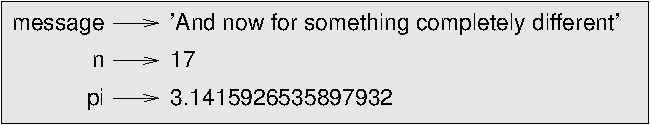
\includegraphics[scale=0.8]{../source/figs/state2.pdf}}
\caption{State diagram.  |  状态图。}
\label{fig.state2}
\end{figure}



\section{Variable names  |  变量名}
\index{variable}

Programmers generally choose names for their variables that
are meaningful---they document what the variable is used for.

Variable names can be as long as you like.  They can contain
both letters and numbers, but they can't begin with a number.
It is legal to use uppercase letters, but it is conventional
to use only lower case for variables names.

The underscore character, \verb"_", can appear in a name.
It is often used in names with multiple words, such as
\verb"your_name" or \verb"airspeed_of_unladen_swallow".
\index{underscore character}

If you give a variable an illegal name, you get a syntax error:

程序员通常为变量选择有意义的名字—它们可以记录该变量的用途。

变量名可以任意长。它们可以包括字母和数字,但是不能以数字开头。 使用大写字母是合法的,但是根据惯例,变量名只使用小写字母。

下划线 \lstinline{_} 可以出现在变量名中。 它经常用于有多个单词的变量名,例如 \lstinline{my_name} 或者 \lstinline{airspeed_of_unladen_swallow}。

如果你给了变量一个非法的名称,解释器将抛出一个语法错误:

\begin{lstlisting}
>>> 76trombones = 'big parade'
SyntaxError: invalid syntax
>>> more@ = 1000000
SyntaxError: invalid syntax
>>> class = 'Advanced Theoretical Zymurgy'
SyntaxError: invalid syntax
\end{lstlisting}
%
{\tt 76trombones} is illegal because it begins with a number.
{\tt more@} is illegal because it contains an illegal character, {\tt
@}.  But what's wrong with {\tt class}?

It turns out that {\tt class} is one of Python's {\bf keywords}.  The
interpreter uses keywords to recognize the structure of the program,
and they cannot be used as variable names.
\index{keyword}

Python 3 has these keywords:

\lstinline{76trombones} 是非法的,因为它以数字开头。 \lstinline{more@} 因为包含了一个非法字符\lstinline{@}也是非法的。 但是,\lstinline{class} 错在哪儿了呢?

原来,\lstinline{class} 是 Python 的 \emph{关键字} (keywords)之一。 解释器使用关键字识别程序的结构,它们不能被用作变量名。

Python 3有以下关键词:


\begin{lstlisting}
False      class      finally    is         return
None       continue   for        lambda     try
True       def        from       nonlocal   while
and        del        global     not        with
as         elif       if         or         yield
assert     else       import     pass
break      except     in         raise
\end{lstlisting}
%
You don't have to memorize this list.  In most development environments,
keywords are displayed in a different color; if you try to use one
as a variable name, you'll know.

你没有必要背诵上面的关键词。大部分的开发环境会用不同的颜色区别显示关键词;如果你不小心使用关键词作为变量名,你肯定会发现的。

\section{Expressions and statements  |  表达式和语句}

An {\bf expression} is a combination of values, variables, and operators.
A value all by itself is considered an expression, and so is
a variable, so the following are all legal expressions:

\emph{表达式} (expression) 是值、变量和运算符的组合。 值自身也被认为是一个表达式,变量也是,因此下面都是合法的表达式:
\index{expression}  \index{表达式}

\begin{lstlisting}
>>> 42
42
>>> n
17
>>> n + 25
42
\end{lstlisting}
%
When you type an expression at the prompt, the interpreter
{\bf evaluates} it, which means that it finds the value of
the expression.
In this example, {\tt n} has the value 17 and
{\tt n + 25} has the value 42.
\index{evaluate}

A {\bf statement} is a unit of code that has an effect, like
creating a variable or displaying a value.
\index{statement}

当你在提示符后输入表达式时,解释器会 \emph{计算} (evaluate) 该表达式,这就意味着解释器会求它的值。在上面的例子中,\lstinline{n} 的值是 \lstinline{17,n + 25} 的值是 \lstinline{42}。

\emph{语句} (statement) 是一个会产生影响的代码单元,例如新建一个变量或显示某个值。

\begin{lstlisting}
>>> n = 17
>>> print(n)
\end{lstlisting}
%
The first line is an assignment statement that gives a value to
{\tt n}.  The second line is a print statement that displays the
value of {\tt n}.

When you type a statement, the interpreter {\bf executes} it,
which means that it does whatever the statement says.  In general,
statements don't have values.
\index{execute}

第一行是一个赋值语句,将某个值赋给了 \lstinline{n}。第二行是一个打印语句,在屏幕上显示 \lstinline{n} 的值。

当你输入一个语句后,解释器会 \emph{执行} (execute) 这个语句,即按照语句的指令完成操作。一般来说,语句是没有值的。
\index{execute}

\section{Script mode  |  脚本模式}

So far we have run Python in {\bf interactive mode}, which
means that you interact directly with the interpreter.
Interactive mode is a good way to get started,
but if you are working with more than a few lines of code, it can be
clumsy.

The alternative is to save code in a file called a {\bf script} and
then run the interpreter in {\bf script mode} to execute the script.  By
convention, Python scripts have names that end with {\tt .py}.
\index{script}  \index{script mode}

到目前为止,我们都是在\emph{交互模式} (interactive mode) 下运行 Python,即直接与解释器进行交互。交互模式对学习入门很有帮助,但是如果你需要编写很多行代码,使用交互模式就不太方便了。
\index{interactive mode}

另一种方法是将代码保存到一个被称为脚本 (script) 的文件里,然后以脚本模式 (script mode) 运行解释器并执行脚本。按照惯例,Python脚本文件名的后缀是 \lstinline{.py}。
\index{script}  \index{script mode}

If you know how to create and run a script on your computer, you
are ready to go.  Otherwise I recommend using PythonAnywhere again.
I have posted instructions for running in script mode at
\url{http://tinyurl.com/thinkpython2e}.

Because Python provides both modes,
you can test bits of code in interactive mode before you put them
in a script.  But there are differences between interactive mode
and script mode that can be confusing.
\index{interactive mode}  \index{script mode}

如果你知道如何在本地电脑新建并运行脚本,那你可以开始编码了。否则的话,我再次建议使用PythonAnywhere。我在 \href{http://tinyurl.com/thinkpython2e}{http://tinyurl.com/thinkpython2e} 上贴出了如何以脚本模式运行解释器的指南。

由于Python支持这两种模式,在将代码写入脚本之前,你可以在交互模式下对代码片段进行测试。不过,交互模式和脚本模式之间存在一些差异,可能会让你感到疑惑。

For example, if you are using Python as a calculator, you might type

举个例子,如果你把Python当计算器使用,你可能会输入下面这样的代码:

\begin{lstlisting}
>>> miles = 26.2
>>> miles * 1.61
42.182
\end{lstlisting}

The first line assigns a value to {\tt miles}, but it has no visible
effect.  The second line is an expression, so the
interpreter evaluates it and displays the result.  It turns out that a
marathon is about 42 kilometers.

But if you type the same code into a script and run it, you get no
output at all.  In script mode an expression, all by itself, has no
visible effect.  Python actually evaluates the expression, but it doesn't
display the value unless you tell it to:

第一行将一个值赋给 \lstinline{miles},但是并没有产生可见的效果。 第二行是一个表达式,因此解释器计算它并将结果显示出来。 结果告诉我们,一段马拉松大概是 \lstinline{42} 公里。

但是如果你将相同的代码键入一个脚本并且运行它,你得不到任何输出。 在脚本模式下,表达式自身不会产生可见的效果。虽然Python实际上计算了表达式,但是如果你不告诉它要显示结果,它是不会那么做的。

\begin{lstlisting}
miles = 26.2
print(miles * 1.61)
\end{lstlisting}

This behavior can be confusing at first.

A script usually contains a sequence of statements.  If there
is more than one statement, the results appear one at a time
as the statements execute.

For example, the script

这个行为开始可能有些令人费解。

一个脚本通常包括一系列语句。 如果有多于一条的语句,那么随着语句逐个执行,解释器会逐一显示计算结果。

例如,以下脚本

\begin{lstlisting}
print(1)
x = 2
print(x)
\end{lstlisting}
%
produces the output

产生的输出结果是

\begin{lstlisting}
1
2
\end{lstlisting}
%
The assignment statement produces no output.

To check your understanding, type the following statements in the
Python interpreter and see what they do:

赋值语句不产生输出。

在Python解释器中键入以下的语句,看看他们的结果是否符合你的理解:

\begin{lstlisting}
5
x = 5
x + 1
\end{lstlisting}

Now put the same statements in a script and run it.  What
is the output?  Modify the script by transforming each
expression into a print statement and then run it again.

现在将同样的语句写入一个脚本中并执行它。输出结果是什么? 修改脚本,将每个表达式变成打印语句,再次运行它。

\section{Order of operations  |  运算顺序}
\index{order of operations}  \index{PEMDAS}

When an expression contains more than one operator, the order of
evaluation depends on the {\bf order of operations}.  For
mathematical operators, Python follows mathematical convention.
The acronym {\bf PEMDAS} is a useful way to
remember the rules:

当一个表达式中有多于一个运算符时,计算的顺序由 \emph{运算顺序} (order of operations) 决定。 对于算数运算符,Python遵循数学里的惯例。 缩写\textbf{PEMDAS}有助于帮助大家记住这些规则:

\begin{itemize}

\item {\bf P}arentheses have the highest precedence and can be used
to force an expression to evaluate in the order you want. Since
expressions in parentheses are evaluated first, {\tt 2 * (3-1)} is 4,
and {\tt (1+1)**(5-2)} is 8. You can also use parentheses to make an
expression easier to read, as in {\tt (minute * 100) / 60}, even
if it doesn't change the result.

\item {\bf E}xponentiation has the next highest precedence, so
{\tt 1 + 2**3} is 9, not 27, and {\tt 2 * 3**2} is 18, not 36.

\item {\bf M}ultiplication and {\bf D}ivision have higher precedence
  than {\bf A}ddition and {\bf S}ubtraction.  So {\tt 2*3-1} is 5, not
  4, and {\tt 6+4/2} is 8, not 5.

\item Operators with the same precedence are evaluated from left to
  right (except exponentiation).  So in the expression {\tt degrees /
    2 * pi}, the division happens first and the result is multiplied
  by {\tt pi}.  To divide by $2 \pi$, you can use parentheses or write
  {\tt degrees / 2 / pi}.

\end{itemize}

\begin{itemize}

\item \emph{括号} (\textbf{P}arentheses) 具有最高的优先级,并且可以强制表达式按你希望的顺序计算。 因为在括号中的表达式首先被计算,那么 \lstinline{2 * (3-1)} 的结果是 \lstinline{4},\lstinline{(1+1)**(5-2)} 的结果是 \lstinline{8}。 你也可以用括号提高表达式的可读性,如写成 \lstinline{(minute * 100) / 60},即使这样并不改变运算的结果。

\item \emph{指数运算} (\textbf{E}xponentiation) 具有次高的优先级,因此 \lstinline{1 + 2**3} 的结果是 \lstinline{9} 而非 \lstinline{27}, \lstinline{2 * 3**2} 的结果是 \lstinline{18} 而非 \lstinline{36}。

\item \emph{乘法} (\textbf{M}ultiplication) 和 \emph{除法} (\textbf{D}ivision) 有相同的优先级, 比 \emph{加法} (Addition) 和 \emph{减法} (Subtraction) 高,加法和减法也具有相同的优先级。 因此 \lstinline{2*3-1} 是 \lstinline{5} 而非 \lstinline{4}, \lstinline{6+4/2} 是 \lstinline{8} 而非 \lstinline{5}。

\item 具有相同优先级的运算符按照从左到右的顺序进行计算(除了指数运算)。 因此表达式 \lstinline{degrees / 2 * pi} 中,除法先运算,然后结果被乘以 \lstinline{pi}。 为了被 $2\pi$ 除,你可以使用括号,或者写成 \lstinline{degrees / 2 / pi}。

\end{itemize}

I don't work very hard to remember the precedence of
operators.  If I can't tell by looking at the expression, I use
parentheses to make it obvious.

我不会费力去记住这些运算符的优先级规则。如果看完表达式后分不出优先级,我会使用括号使计算顺序变得更明显。


%
\section{String operations  |  字符串运算}
\index{string!operation}  \index{operator!string}
\index{字符串!操作}  \index{操作!字符串}

In general, you can't perform mathematical operations on strings, even
if the strings look like numbers, so the following are illegal:

一般来讲,你不能对字符串执行数学运算,即使字符串看起来很像数字, 因此下面这些表达式是非法的:


\begin{lstlisting}
'2'-'1'    'eggs'/'easy'    'third'*'a charm'
\end{lstlisting}
%
But there are two exceptions, {\tt +} and {\tt *}.

The {\tt +} operator performs {\bf string concatenation}, which means
it joins the strings by linking them end-to-end.  For example:

但有两个例外,+ 和 *。

加号运算符 \lstinline{+} 可用于 字符串拼接 (string concatenation),也就是将字符串首尾相连起来。例如:
\index{concatenation}

\begin{lstlisting}
>>> first = 'throat'
>>> second = 'warbler'
>>> first + second
throatwarbler
\end{lstlisting}
%
The {\tt *} operator also works on strings; it performs repetition.
For example, \verb"'Spam'*3" is \verb"'SpamSpamSpam'".  If one of the
values is a string, the other has to be an integer.

This use of {\tt +} and {\tt *} makes sense by
analogy with addition and multiplication.  Just as {\tt 4*3} is
equivalent to {\tt 4+4+4}, we expect \verb"'Spam'*3" to be the same as
\verb"'Spam'+'Spam'+'Spam'", and it is.  On the other hand, there is a
significant way in which string concatenation and repetition are
different from integer addition and multiplication.
Can you think of a property that addition has
that string concatenation does not?
\index{commutativity}

乘法运算符 \lstinline{*} 也可应用于字符串;它执行重复运算。 例如,\lstinline{'Spam'*3} 的结果是 \lstinline{'SpamSpamSpam'}。  如果其中一个运算数是字符串,则另外一个必须是整型数。

\lstinline{+} 和 \lstinline{*} 的这个用法,类比加法和乘法也讲得通。 就像 \lstinline{4*3} 与 \lstinline{4+4+4} 等价一样, 我们也会期望 \lstinline{'Spam'*3} 和 \lstinline{'Spam'+'Spam'+'Spam'} 等价,而事实上的确如此。 另一方面,字符串拼接和重复与整数的加法和乘法也有很大的不同。 你能想出来一个加法具有而字符串拼接不具有的特性么?


\section{Comments  |  注释}
\index{comment}

As programs get bigger and more complicated, they get more difficult
to read.  Formal languages are dense, and it is often difficult to
look at a piece of code and figure out what it is doing, or why.

For this reason, it is a good idea to add notes to your programs to explain
in natural language what the program is doing.  These notes are called
{\bf comments}, and they start with the \verb"#" symbol:

随着程序变得越来越大,越来越复杂,它们的可读性也越来越差。 形式语言是稠密的,通常很难在读一段代码后,说出其做什么或者为什么这样做。

因此,在你的程序中用自然语言做笔记,解释程序做什么通常是比较好的办法。 这些标注被称为\emph{注释} (comments),以 \lstinline{#} 符号开始。

\begin{lstlisting}
# compute the percentage of the hour that has elapsed
# 计算逝去的时间占一小时的比例
percentage = (minute * 100) / 60
\end{lstlisting}
%
In this case, the comment appears on a line by itself.  You can also put
comments at the end of a line:

此例中,注释独立一行。你也可以将注释放在行尾:

\begin{lstlisting}
percentage = (minute * 100) / 60     # percentage of an hour
\end{lstlisting}
%
Everything from the {\tt \#} to the end of the line is ignored---it
has no effect on the execution of the program.

Comments are most useful when they document non-obvious features of
the code.  It is reasonable to assume that the reader can figure out
{\em what} the code does; it is more useful to explain {\em why}.

This comment is redundant with the code and useless:

从 \lstinline{#} 开始到行尾的所有内容都会被解释器忽略—其对程序执行没有影响。

在注释中记录代码不明显的特征,是最有帮助的。 假设读者能够读懂代码做了\textbf{什么}是合理的; 但是解释代码\textbf{为什么}这么做则更有用。

下面这个注释只是重复了代码,没有什么用:

\begin{lstlisting}
v = 5     # assign 5 to v
\end{lstlisting}
%
This comment contains useful information that is not in the code:

下面的注释包括了代码中没有的有用信息:

\begin{lstlisting}
v = 5     # velocity in meters/second.
\end{lstlisting}
%
Good variable names can reduce the need for comments, but
long names can make complex expressions hard to read, so there is
a tradeoff.

好的变量名能够减少对注释的需求,但是长变量名使得表达式很难读, 因此这里有个平衡问题。

%
\section{Debugging  |  调试}
\index{debugging}  \index{bug}
\index{调试}  \index{故障}

Three kinds of errors can occur in a program: syntax errors, runtime
errors, and semantic errors.  It is useful
to distinguish between them in order to track them down more quickly.

程序中可能会出现下面三种错误:\emph{语法错误} (syntax error)、 \emph{运行时错误} (runtime error) 和 \emph{语义错误} (semantic error)。 区别三者的差异有助于快速追踪这些错误。

\begin{description}

\item[Syntax error:] ``Syntax'' refers to the structure of a program
  and the rules about that structure.  For example, parentheses have
  to come in matching pairs, so {\tt (1 + 2)} is legal, but {\tt 8)}
  is a {\bf syntax error}.  \index{syntax error} \index{error!syntax}
  \index{error message}
\index{syntax}

If there is a syntax error
anywhere in your program, Python displays an error message and quits,
and you will not be able to run the program.  During the first few
weeks of your programming career, you might spend a lot of
time tracking down syntax errors.  As you gain experience, you will
make fewer errors and find them faster.


\item[Runtime error:] The second type of error is a runtime error, so
  called because the error does not appear until after the program has
  started running.  These errors are also called {\bf exceptions}
  because they usually indicate that something exceptional (and bad)
  has happened.  \index{runtime error} \index{error!runtime}
  \index{exception} \index{safe language} \index{language!safe}

Runtime errors are rare in the simple programs you will see in the
first few chapters, so it might be a while before you encounter one.


\item[Semantic error:] The third type of error is ``semantic'', which
  means related to meaning.  If there is a semantic error in your
  program, it will run without generating error messages, but it will
  not do the right thing.  It will do something else.  Specifically,
  it will do what you told it to do.  \index{semantic error}
  \index{error!semantic} \index{error message}

Identifying semantic errors can be tricky because it requires you to work
backward by looking at the output of the program and trying to figure
out what it is doing.

\end{description}

\begin{description}

\item[语法错误:] 语法指的是程序的结构及其背后的规则。例如,括号必须要成对出现,所以 \lstinline{(1 + 2)} 是合法的,但是 \lstinline{8)} 则是一个 语法错误。
\index{syntax}

如果你的程序中存在一个语法错误,Python会显示一条错误信息,然后退出运行。你无法顺利运行程序。在你编程生涯的头几周里,你可能会花大量时间追踪语法错误。随着你的经验不断积累,犯的语法错误会越来越少,发现错误的速度也会更快。


\item[运行时错误:] 第二种错误类型是运行时错误,这么称呼是因为这类错误只有在程序开始运行后才会出现。这类错误也被称为 \emph{异常} (exception) ,因为它们的出现通常说明发生了某些特别的(而且不好的)事情。
  \index{runtime error} \index{error!runtime}
  \index{exception} \index{safe language} \index{language!safe}

在前几章提供的简单程序中,你很少会碰到运行时错误,所以你可能需要一段时间才会接触到这种错误。




\item[语义错误:] 第三类错误是“语义”错误,即与程序的意思的有关。如果你的程序中有语义错误,程序在运行时不会产生错误信息,但是不会返回正确的结果。它会返回另外的结果。严格来说,它是按照你的指令在运行。
  \index{semantic error}  \index{error!semantic}  \index{error message}

识别语义错误可能是棘手的,因为这需要你反过来思考,通过观察程序的输出来搞清楚它在做什么。

\end{description}



\section{Glossary  |  术语表}

\begin{description}

\item[variable:]  A name that refers to a value.
\index{variable}

\item[assignment:]  A statement that assigns a value to a variable.
\index{assignment}

\item[state diagram:]  A graphical representation of a set of variables and the
values they refer to.
\index{state diagram}

\item[keyword:]  A reserved word that is used to parse a
program; you cannot use keywords like {\tt if}, {\tt  def}, and {\tt while} as
variable names.
\index{keyword}

\item[operand:]  One of the values on which an operator operates.
\index{operand}

\item[expression:]  A combination of variables, operators, and values that
represents a single result.
\index{expression}

\item[evaluate:]  To simplify an expression by performing the operations
in order to yield a single value.

\item[statement:]  A section of code that represents a command or action.  So
far, the statements we have seen are assignments and print statements.
\index{statement}

\item[execute:]  To run a statement and do what it says.
\index{execute}

\item[interactive mode:] A way of using the Python interpreter by
typing code at the prompt.
\index{interactive mode}

\item[script mode:] A way of using the Python interpreter to read
code from a script and run it.
\index{script mode}

\item[script:] A program stored in a file.
\index{script}

\item[order of operations:]  Rules governing the order in which
expressions involving multiple operators and operands are evaluated.
\index{order of operations}

\item[concatenate:]  To join two operands end-to-end.
\index{concatenation}

\item[comment:]  Information in a program that is meant for other
programmers (or anyone reading the source code) and has no effect on the
execution of the program.
\index{comment}

\item[syntax error:]  An error in a program that makes it impossible
to parse (and therefore impossible to interpret).
\index{syntax error}

\item[exception:]  An error that is detected while the program is running.
\index{exception}

\item[semantics:]  The meaning of a program.
\index{semantics}

\item[semantic error:]   An error in a program that makes it do something
other than what the programmer intended.
\index{semantic error}

\end{description}

\begin{description}

\item[变量 (variable):]  变量是指向某个值的名称。
\index{variable}  \index{变量}

\item[赋值语句 (assignment):]  将某个值赋给变量的语句。
\index{assignment}  \index{赋值语句}

\item[状态图 (state diagram):]  变量及其所指的值的图形化表示。
\index{state diagram}  \index{状态图}

\item[关键字 (keyword):]  关键字是用于解析程序的;你不能使用if、def和while这样的关键词作为变量名。
\index{keyword}  \index{关键字}

\item[运算数 (operand):]  运算符所操作的值之一。
\index{operand}  \index{运算数}

\item[表达式 (expression):]  变量、运算符和值的组合,代表一个单一的结果。
\index{expression}  \index{表达式}

\item[计算 (evaluate):]  通过执行运算以简化表达式,从而得出一个单一的值。

\item[语句 (statement):]  代表一个命令或行为的一段代码。 目前为止我们接触的语句有赋值语句和打印语句。
\index{statement}  \index{语句}

\item[执行 (execute):]  运行一个语句,并按照语句的指令操作。
\index{execute}  \index{执行}

\item[交互式模式 (interactive mode):]  通过在提示符中输入代码,使用Python解释器的一种方式。
\index{interactive mode}  \index{交互式模式}

\item[脚本模式 (script mode):]  使用Python解释器从脚本中读取代码,并运行脚本的方式。
\index{script mode}  \index{脚本模式}

\item[脚本 (script):]  保存在文件中的程序。
\index{script}  \index{脚本}

\item[运算顺序 (order of operations):]  有关多个运算符和运算数时计算顺序的规则。
\index{order of operations}  \index{运算顺序}

\item[拼接 (concatenate):]  将两个运算数首尾相连。
\index{concatenation}  \index{拼接}

\item[注释 (comment):]  程序中提供给其他程序员(任何阅读源代码的人)阅读的信息,对程序的执行没有影响。
\index{comment}  \index{注释}

\item[语法错误 (syntax error):]  使得程序无法进行解析(因此无法进行解释)的错误。
\index{syntax error}  \index{语法错误}

\item[异常 (exception):]  只有在程序运行时才发现的错误。
\index{exception}  \index{异常}

\item[语义 (semantics):]  程序中表达的意思。
\index{semantics}  \index{语义}

\item[语义错误 (semantic error):]  使得程序偏离程序员原本期望的错误。
\index{semantic error}  \index{语义错误}

\end{description}


\section{Exercises  |  练习}

\begin{exercise}

Repeating my advice from the previous chapter, whenever you learn
a new feature, you should try it out in interactive mode and make
errors on purpose to see what goes wrong.

\begin{itemize}

\item We've seen that {\tt n = 42} is legal.  What about {\tt 42 = n}?

\item How about {\tt x = y = 1}?

\item In some languages every statement ends with a semi-colon, {\tt ;}.
What happens if you put a semi-colon at the end of a Python statement?

\item What if you put a period at the end of a statement?

\item In math notation you can multiply $x$ and $y$ like this: $x y$.
What happens if you try that in Python?

\end{itemize}

和上一章一样,我还是要建议大家在学习新特性之后,在交互模式下充分试验,故意犯一些错误,看看到底会出什么问题。

\begin{itemize}

\item 我们已经知道 \lstinline{n = 42} 是合法的。那么 \lstinline{42 = n} 呢?

\item \lstinline{x = y = 1} 合法吗?

\item 在某些编程语言中,每个语句都是以分号 \lstinline{;} 结束的。如果你在一个Python语句后也以分号结尾,会发生什么?

\item 如果在语句最后带上分号呢?

\item 在数学记法中,你可以将  $x$ 和  $y$ 像这样相乘: $x y$ 。如果你在 Python 中也这么写的话,会发生什么?

\end{exercise}


\begin{exercise}

Practice using the Python interpreter as a calculator:
\index{calculator}

\begin{enumerate}

\item The volume of a sphere with radius $r$ is $\frac{4}{3} \pi r^3$.
  What is the volume of a sphere with radius 5?

\item Suppose the cover price of a book is \$24.95, but bookstores get a
  40\% discount.  Shipping costs \$3 for the first copy and 75 cents
  for each additional copy.  What is the total wholesale cost for
  60 copies?

\item If I leave my house at 6:52 am and run 1 mile at an easy pace
  (8:15 per mile), then 3 miles at tempo (7:12 per mile) and 1 mile at
  easy pace again, what time do I get home for breakfast?
\index{running pace}

\end{enumerate}

继续练习将 Python 解释器当做计算器使用:

\begin{enumerate}

\item 半径为 $r$ 的球体积是 $\frac{4}{3} \pi r^3$ 。 半径为 $5$ 的球体积是多少?

\item 假设一本书的零售价是 \$24.95,但书店有 40\% 的折扣。运费则是第一本 \$3 ,以后每本 75 美分。 购买 60 本的总价是多少?

\item 如果我上午 6:52 离开家, 以轻松跑 (easy pace)的速度跑 1 英里(即每英里耗时8分15秒),再以节奏跑(tempo)的速度跑3英里(每英里耗时7分12秒),之后又以放松跑的速度跑1英里,我什么时候回到家吃早饭? \footnote{译者注:配速(pace)是在马拉松运动的训练中常使用的一个概念,配速是速度的一种,是每公里所需要的时间。配速=时间/距离。Tempo run一般被翻译成「节奏跑」或「乳酸门槛跑」,是指以比10K或5K比赛速度稍慢(每公里大约慢10-15秒)的速度进行训练,或者以平时15K-半程的配速来跑。参考:https://www.zhihu.com/question/22237002}
\index{running pace}

\end{enumerate}

\end{exercise}


\chapter{Functions}
\label{funcchap}

In the context of programming, a {\bf function} is a named sequence of
statements that performs a computation.  When you define a function,
you specify the name and the sequence of statements.  Later, you can
``call'' the function by name.
\index{function}

\section{Function calls}
\label{functionchap}
\index{function call}

We have already seen one example of a {\bf function call}:

\begin{verbatim}
>>> type(42)
<class 'int'>
\end{verbatim}
%
The name of the function is {\tt type}.  The expression in parentheses
is called the {\bf argument} of the function.  The result, for this
function, is the type of the argument.
\index{parentheses!argument in}

It is common to say that a function ``takes'' an argument and ``returns''
a result.  The result is also called the {\bf return value}.
\index{argument}
\index{return value}

Python provides functions that convert values
from one type to another.  The {\tt int} function takes any value and
converts it to an integer, if it can, or complains otherwise:
\index{conversion!type}
\index{type conversion}
\index{int function}
\index{function!int}

\begin{verbatim}
>>> int('32')
32
>>> int('Hello')
ValueError: invalid literal for int(): Hello
\end{verbatim}
%
{\tt int} can convert floating-point values to integers, but it
doesn't round off; it chops off the fraction part:

\begin{verbatim}
>>> int(3.99999)
3
>>> int(-2.3)
-2
\end{verbatim}
%
{\tt float} converts integers and strings to floating-point
numbers:
\index{float function}
\index{function!float}

\begin{verbatim}
>>> float(32)
32.0
>>> float('3.14159')
3.14159
\end{verbatim}
%
Finally, {\tt str} converts its argument to a string:
\index{str function}
\index{function!str}

\begin{verbatim}
>>> str(32)
'32'
>>> str(3.14159)
'3.14159'
\end{verbatim}
%

\section{Math functions}
\index{math function}
\index{function, math}

Python has a math module that provides most of the familiar
mathematical functions.  A {\bf module} is a file that contains a
collection of related functions.
\index{module}
\index{module object}

Before we can use the functions in a module, we have to import it with
an {\bf import statement}:

\begin{verbatim}
>>> import math
\end{verbatim}
%
This statement creates a {\bf module object} named math.  If
you display the module object, you get some information about it:

\begin{verbatim}
>>> math
<module 'math' (built-in)>
\end{verbatim}
%
The module object contains the functions and variables defined in the
module.  To access one of the functions, you have to specify the name
of the module and the name of the function, separated by a dot (also
known as a period).  This format is called {\bf dot notation}.
\index{dot notation}

\begin{verbatim}
>>> ratio = signal_power / noise_power
>>> decibels = 10 * math.log10(ratio)

>>> radians = 0.7
>>> height = math.sin(radians)
\end{verbatim}
%
The first example uses \verb"math.log10" to compute
a signal-to-noise ratio in decibels (assuming that \verb"signal_power" and
\verb"noise_power" are defined).  The math module also provides {\tt log},
which computes logarithms base {\tt e}.
\index{log function}
\index{function!log}
\index{sine function}
\index{radian}
\index{trigonometric function}
\index{function, trigonometric}

The second example finds the sine of {\tt radians}.  The name of the
variable is a hint that {\tt sin} and the other trigonometric
functions ({\tt cos}, {\tt tan}, etc.)  take arguments in radians. To
convert from degrees to radians, divide by 180 and multiply by
$\pi$:

\begin{verbatim}
>>> degrees = 45
>>> radians = degrees / 180.0 * math.pi
>>> math.sin(radians)
0.707106781187
\end{verbatim}
%
The expression {\tt math.pi} gets the variable {\tt pi} from the math
module.  Its value is a floating-point approximation
of $\pi$, accurate to about 15 digits.
\index{pi}

If you know
trigonometry, you can check the previous result by comparing it to
the square root of two divided by two:
\index{sqrt function}
\index{function!sqrt}

\begin{verbatim}
>>> math.sqrt(2) / 2.0
0.707106781187
\end{verbatim}
%

\section{Composition}
\index{composition}

So far, we have looked at the elements of a program---variables,
expressions, and statements---in isolation, without talking about how to
combine them.

One of the most useful features of programming languages is their
ability to take small building blocks and {\bf compose} them.  For
example, the argument of a function can be any kind of expression,
including arithmetic operators:

\begin{verbatim}
x = math.sin(degrees / 360.0 * 2 * math.pi)
\end{verbatim}
%
And even function calls:

\begin{verbatim}
x = math.exp(math.log(x+1))
\end{verbatim}
%
Almost anywhere you can put a value, you can put an arbitrary
expression, with one exception: the left side of an assignment
statement has to be a variable name.  Any other expression on the left
side is a syntax error (we will see exceptions to this rule
later).

\begin{verbatim}
>>> minutes = hours * 60                 # right
>>> hours * 60 = minutes                 # wrong!
SyntaxError: can't assign to operator
\end{verbatim}
%
\index{SyntaxError}
\index{exception!SyntaxError}


\section{Adding new functions}

So far, we have only been using the functions that come with Python,
but it is also possible to add new functions.
A {\bf function definition} specifies the name of a new function and
the sequence of statements that run when the function is called.
\index{function}
\index{function definition}
\index{definition!function}

Here is an example:

\begin{verbatim}
def print_lyrics():
    print("I'm a lumberjack, and I'm okay.")
    print("I sleep all night and I work all day.")
\end{verbatim}
%
{\tt def} is a keyword that indicates that this is a function
definition.  The name of the function is \verb"print_lyrics".  The
rules for function names are the same as for variable names: letters,
numbers and underscore are legal, but the first character
can't be a number.  You can't use a keyword as the name of a function,
and you should avoid having a variable and a function with the same
name.
\index{def keyword}
\index{keyword!def}
\index{argument}

The empty parentheses after the name indicate that this function
doesn't take any arguments.
\index{parentheses!empty}
\index{header}
\index{body}
\index{indentation}
\index{colon}

The first line of the function definition is called the {\bf header};
the rest is called the {\bf body}.  The header has to end with a colon
and the body has to be indented.  By convention, indentation is
always four spaces.  The body can contain
any number of statements.

The strings in the print statements are enclosed in double
quotes.  Single quotes and double quotes do the same thing;
most people use single quotes except in cases like this where
a single quote (which is also an apostrophe) appears in the string.

All quotation marks (single and double)
must be ``straight quotes'', usually
located next to Enter on the keyboard.  ``Curly quotes'', like
the ones in this sentence, are not legal in Python.

If you type a function definition in interactive mode, the interpreter
prints dots ({\tt ...}) to let you know that the definition
isn't complete:
\index{ellipses}

\begin{verbatim}
>>> def print_lyrics():
...     print("I'm a lumberjack, and I'm okay.")
...     print("I sleep all night and I work all day.")
...
\end{verbatim}
%
To end the function, you have to enter an empty line.

Defining a function creates a {\bf function object}, which
has type \verb"function":
\index{function type}
\index{type!function}

\begin{verbatim}
>>> print(print_lyrics)
<function print_lyrics at 0xb7e99e9c>
>>> type(print_lyrics)
<class 'function'>
\end{verbatim}
%
The syntax for calling the new function is the same as
for built-in functions:

\begin{verbatim}
>>> print_lyrics()
I'm a lumberjack, and I'm okay.
I sleep all night and I work all day.
\end{verbatim}
%
Once you have defined a function, you can use it inside another
function.  For example, to repeat the previous refrain, we could write
a function called \verb"repeat_lyrics":

\begin{verbatim}
def repeat_lyrics():
    print_lyrics()
    print_lyrics()
\end{verbatim}
%
And then call \verb"repeat_lyrics":

\begin{verbatim}
>>> repeat_lyrics()
I'm a lumberjack, and I'm okay.
I sleep all night and I work all day.
I'm a lumberjack, and I'm okay.
I sleep all night and I work all day.
\end{verbatim}
%
But that's not really how the song goes.


\section{Definitions and uses}
\index{function definition}

Pulling together the code fragments from the previous section, the
whole program looks like this:

\begin{verbatim}
def print_lyrics():
    print("I'm a lumberjack, and I'm okay.")
    print("I sleep all night and I work all day.")

def repeat_lyrics():
    print_lyrics()
    print_lyrics()

repeat_lyrics()
\end{verbatim}
%
This program contains two function definitions: \verb"print_lyrics" and
\verb"repeat_lyrics".  Function definitions get executed just like other
statements, but the effect is to create function objects.  The statements
inside the function do not run until the function is called, and
the function definition generates no output.
\index{use before def}

As you might expect, you have to create a function before you can
run it.  In other words, the function definition has to run
before the function gets called.

As an exercise, move the last line of this program
to the top, so the function call appears before the definitions. Run
the program and see what error
message you get.

Now move the function call back to the bottom
and move the definition of \verb"print_lyrics" after the definition of
\verb"repeat_lyrics".  What happens when you run this program?


\section{Flow of execution}
\index{flow of execution}

To ensure that a function is defined before its first use,
you have to know the order statements run in, which is
called the {\bf flow of execution}.

Execution always begins at the first statement of the program.
Statements are run one at a time, in order from top to bottom.

Function definitions do not alter the flow of execution of the
program, but remember that statements inside the function don't
run until the function is called.

A function call is like a detour in the flow of execution. Instead of
going to the next statement, the flow jumps to the body of
the function, runs the statements there, and then comes back
to pick up where it left off.

That sounds simple enough, until you remember that one function can
call another.  While in the middle of one function, the program might
have to run the statements in another function.  Then, while
running that new function, the program might have to run yet
another function!

Fortunately, Python is good at keeping track of where it is, so each
time a function completes, the program picks up where it left off in
the function that called it.  When it gets to the end of the program,
it terminates.

In summary, when you read a program, you
don't always want to read from top to bottom.  Sometimes it makes
more sense if you follow the flow of execution.


\section{Parameters and arguments}
\label{parameters}
\index{parameter}
\index{function parameter}
\index{argument}
\index{function argument}

Some of the functions we have seen require arguments.  For
example, when you call {\tt math.sin} you pass a number
as an argument.  Some functions take more than one argument:
{\tt math.pow} takes two, the base and the exponent.

Inside the function, the arguments are assigned to
variables called {\bf parameters}.  Here is a definition for
a function that takes an argument:
\index{parentheses!parameters in}

\begin{verbatim}
def print_twice(bruce):
    print(bruce)
    print(bruce)
\end{verbatim}
%
This function assigns the argument to a parameter
named {\tt bruce}.  When the function is called, it prints the value of
the parameter (whatever it is) twice.

This function works with any value that can be printed.

\begin{verbatim}
>>> print_twice('Spam')
Spam
Spam
>>> print_twice(42)
42
42
>>> print_twice(math.pi)
3.14159265359
3.14159265359
\end{verbatim}
%
The same rules of composition that apply to built-in functions also
apply to programmer-defined functions, so we can use any kind of expression
as an argument for \verb"print_twice":
\index{composition}
\index{programmer-defined function}
\index{function!programmer defined}

\begin{verbatim}
>>> print_twice('Spam '*4)
Spam Spam Spam Spam
Spam Spam Spam Spam
>>> print_twice(math.cos(math.pi))
-1.0
-1.0
\end{verbatim}
%
The argument is evaluated before the function is called, so
in the examples the expressions \verb"'Spam '*4" and
{\tt math.cos(math.pi)} are only evaluated once.
\index{argument}

You can also use a variable as an argument:

\begin{verbatim}
>>> michael = 'Eric, the half a bee.'
>>> print_twice(michael)
Eric, the half a bee.
Eric, the half a bee.
\end{verbatim}
%
The name of the variable we pass as an argument ({\tt michael}) has
nothing to do with the name of the parameter ({\tt bruce}).  It
doesn't matter what the value was called back home (in the caller);
here in \verb"print_twice", we call everybody {\tt bruce}.


\section{Variables and parameters are local}
\index{local variable}
\index{variable!local}

When you create a variable inside a function, it is {\bf local},
which means that it only
exists inside the function.  For example:
\index{parentheses!parameters in}

\begin{verbatim}
def cat_twice(part1, part2):
    cat = part1 + part2
    print_twice(cat)
\end{verbatim}
%
This function takes two arguments, concatenates them, and prints
the result twice.  Here is an example that uses it:
\index{concatenation}

\begin{verbatim}
>>> line1 = 'Bing tiddle '
>>> line2 = 'tiddle bang.'
>>> cat_twice(line1, line2)
Bing tiddle tiddle bang.
Bing tiddle tiddle bang.
\end{verbatim}
%
When \verb"cat_twice" terminates, the variable {\tt cat}
is destroyed.  If we try to print it, we get an exception:
\index{NameError}
\index{exception!NameError}

\begin{verbatim}
>>> print(cat)
NameError: name 'cat' is not defined
\end{verbatim}
%
Parameters are also local.
For example, outside \verb"print_twice", there is no
such thing as {\tt bruce}.
\index{parameter}


\section{Stack diagrams}
\label{stackdiagram}
\index{stack diagram}
\index{function frame}
\index{frame}

To keep track of which variables can be used where, it is sometimes
useful to draw a {\bf stack diagram}.  Like state diagrams, stack
diagrams show the value of each variable, but they also show the
function each variable belongs to.
\index{stack diagram}
\index{diagram!stack}

Each function is represented by a {\bf frame}.  A frame is a box with
the name of a function beside it and the parameters and variables of
the function inside it.  The stack diagram for the previous example is
shown in Figure~\ref{fig.stack}.

\begin{figure}
\centerline
{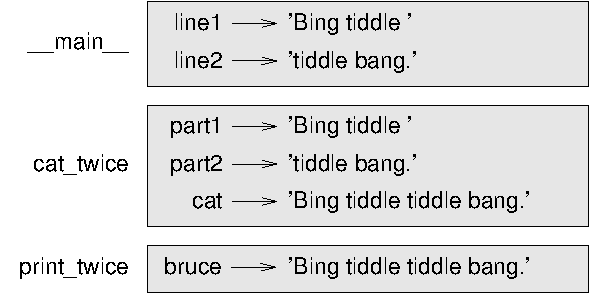
\includegraphics[scale=0.8]{../source/figs/stack.pdf}}
\caption{Stack diagram.}
\label{fig.stack}
\end{figure}


The frames are arranged in a stack that indicates which function
called which, and so on.  In this example, \verb"print_twice"
was called by \verb"cat_twice", and \verb"cat_twice" was called by
\verb"__main__", which is a special name for the topmost frame.  When
you create a variable outside of any function, it belongs to
\verb"__main__".

Each parameter refers to the same value as its corresponding
argument.  So, {\tt part1} has the same value as
{\tt line1}, {\tt part2} has the same value as {\tt line2},
and {\tt bruce} has the same value as {\tt cat}.

If an error occurs during a function call, Python prints the
name of the function, the name of the function that called
it, and the name of the function that called {\em that}, all the
way back to \verb"__main__".

For example, if you try to access {\tt cat} from within
\verb"print_twice", you get a {\tt NameError}:

\begin{verbatim}
Traceback (innermost last):
  File "test.py", line 13, in __main__
    cat_twice(line1, line2)
  File "test.py", line 5, in cat_twice
    print_twice(cat)
  File "test.py", line 9, in print_twice
    print(cat)
NameError: name 'cat' is not defined
\end{verbatim}
%
This list of functions is called a {\bf traceback}.  It tells you what
program file the error occurred in, and what line, and what functions
were executing at the time.  It also shows the line of code that
caused the error.
\index{traceback}

The order of the functions in the traceback is the same as the
order of the frames in the stack diagram.  The function that is
currently running is at the bottom.


\section{Fruitful functions and void functions}
\index{fruitful function}
\index{void function}
\index{function, fruitful}
\index{function, void}

Some of the functions we have used, such as the math functions, return
results; for lack of a better name, I call them {\bf fruitful
  functions}.  Other functions, like \verb"print_twice", perform an
action but don't return a value.  They are called {\bf void
  functions}.

When you call a fruitful function, you almost always
want to do something with the result; for example, you might
assign it to a variable or use it as part of an expression:

\begin{verbatim}
x = math.cos(radians)
golden = (math.sqrt(5) + 1) / 2
\end{verbatim}
%
When you call a function in interactive mode, Python displays
the result:

\begin{verbatim}
>>> math.sqrt(5)
2.2360679774997898
\end{verbatim}
%
But in a script, if you call a fruitful function all by itself,
the return value is lost forever!

\begin{verbatim}
math.sqrt(5)
\end{verbatim}
%
This script computes the square root of 5, but since it doesn't store
or display the result, it is not very useful.
\index{interactive mode}
\index{script mode}

Void functions might display something on the screen or have some
other effect, but they don't have a return value.  If you
assign the result to a variable, you get a special value called
{\tt None}.
\index{None special value}
\index{special value!None}

\begin{verbatim}
>>> result = print_twice('Bing')
Bing
Bing
>>> print(result)
None
\end{verbatim}
%
The value {\tt None} is not the same as the string \verb"'None'".
It is a special value that has its own type:

\begin{verbatim}
>>> print(type(None))
<class 'NoneType'>
\end{verbatim}
%
The functions we have written so far are all void.  We will start
writing fruitful functions in a few chapters.
\index{NoneType type}
\index{type!NoneType}


\section{Why functions?}
\index{function, reasons for}

It may not be clear why it is worth the trouble to divide
a program into functions.  There are several reasons:

\begin{itemize}

\item Creating a new function gives you an opportunity to name a group
of statements, which makes your program easier to read and debug.

\item Functions can make a program smaller by eliminating repetitive
code.  Later, if you make a change, you only have
to make it in one place.

\item Dividing a long program into functions allows you to debug the
parts one at a time and then assemble them into a working whole.

\item Well-designed functions are often useful for many programs.
Once you write and debug one, you can reuse it.

\end{itemize}


\section{Debugging}

One of the most important skills you will acquire is debugging.
Although it can be frustrating, debugging is one of the most
intellectually rich, challenging, and interesting parts of
programming.
\index{experimental debugging}
\index{debugging!experimental}

In some ways debugging is like detective work.  You are confronted
with clues and you have to infer the processes and events that led
to the results you see.

Debugging is also like an experimental science.  Once you have an idea
about what is going wrong, you modify your program and try again.  If
your hypothesis was correct, you can predict the result of the
modification, and you take a step closer to a working program.  If
your hypothesis was wrong, you have to come up with a new one.  As
Sherlock Holmes pointed out, ``When you have eliminated the
impossible, whatever remains, however improbable, must be the truth.''
(A. Conan Doyle, {\em The Sign of Four})
\index{Holmes, Sherlock}
\index{Doyle, Arthur Conan}

For some people, programming and debugging are the same thing.  That
is, programming is the process of gradually debugging a program until
it does what you want.  The idea is that you should start with a
working program and make small modifications,
debugging them as you go.

For example, Linux is an operating system that contains millions of
lines of code, but it started out as a simple program Linus Torvalds
used to explore the Intel 80386 chip.  According to Larry Greenfield,
``One of Linus's earlier projects was a program that would switch
between printing AAAA and BBBB.  This later evolved to Linux.''
({\em The Linux Users' Guide} Beta Version 1).
\index{Linux}


\section{Glossary}

\begin{description}

\item[function:] A named sequence of statements that performs some
useful operation.  Functions may or may not take arguments and may or
may not produce a result.
\index{function}

\item[function definition:]  A statement that creates a new function,
specifying its name, parameters, and the statements it contains.
\index{function definition}

\item[function object:]  A value created by a function definition.
The name of the function is a variable that refers to a function
object.
\index{function definition}

\item[header:] The first line of a function definition.
\index{header}

\item[body:] The sequence of statements inside a function definition.
\index{body}

\item[parameter:] A name used inside a function to refer to the value
passed as an argument.
\index{parameter}

\item[function call:] A statement that runs a function. It
consists of the function name followed by an argument list in
parentheses.
\index{function call}

\item[argument:]  A value provided to a function when the function is called.
This value is assigned to the corresponding parameter in the function.
\index{argument}

\item[local variable:]  A variable defined inside a function.  A local
variable can only be used inside its function.
\index{local variable}

\item[return value:]  The result of a function.  If a function call
is used as an expression, the return value is the value of
the expression.
\index{return value}

\item[fruitful function:] A function that returns a value.
\index{fruitful function}

\item[void function:] A function that always returns {\tt None}.
\index{void function}

\item[{\tt None}:]  A special value returned by void functions.
\index{None special value}
\index{special value!None}

\item[module:] A file that contains a
collection of related functions and other definitions.
\index{module}

\item[import statement:] A statement that reads a module file and creates
a module object.
\index{import statement}
\index{statement!import}

\item[module object:] A value created by an {\tt import} statement
that provides access to the values defined in a module.
\index{module}

\item[dot notation:]  The syntax for calling a function in another
module by specifying the module name followed by a dot (period) and
the function name.
\index{dot notation}

\item[composition:] Using an expression as part of a larger expression,
or a statement as part of a larger statement.
\index{composition}

\item[flow of execution:]  The order statements run in.
\index{flow of execution}

\item[stack diagram:]  A graphical representation of a stack of functions,
their variables, and the values they refer to.
\index{stack diagram}

\item[frame:]  A box in a stack diagram that represents a function call.
It contains the local variables and parameters of the function.
\index{function frame}
\index{frame}

\item[traceback:]  A list of the functions that are executing,
printed when an exception occurs.
\index{traceback}


\end{description}


\section{Exercises}

\begin{exercise}
\index{len function}
\index{function!len}

Write a function named \verb"right_justify" that takes a string
named {\tt s} as a parameter and prints the string with enough
leading spaces so that the last letter of the string is in column 70
of the display.

\begin{verbatim}
>>> right_justify('monty')
                                                                 monty
\end{verbatim}

Hint: Use string concatenation and repetition.  Also,
Python provides a built-in function called {\tt len} that
returns the length of a string, so the value of \verb"len('monty')" is 5.

\end{exercise}


\begin{exercise}
\index{function object}
\index{object!function}

A function object is a value you can assign to a variable
or pass as an argument.  For example, \verb"do_twice" is a function
that takes a function object as an argument and calls it twice:

\begin{verbatim}
def do_twice(f):
    f()
    f()
\end{verbatim}

Here's an example that uses \verb"do_twice" to call a function
named \verb"print_spam" twice.

\begin{verbatim}
def print_spam():
    print('spam')

do_twice(print_spam)
\end{verbatim}

\begin{enumerate}

\item Type this example into a script and test it.

\item Modify \verb"do_twice" so that it takes two arguments, a
function object and a value, and calls the function twice,
passing the value as an argument.

\item Copy the definition of
\verb"print_twice" from earlier in this chapter to your script.

\item Use the modified version of \verb"do_twice" to call
\verb"print_twice" twice, passing \verb"'spam'" as an argument.

\item Define a new function called
\verb"do_four" that takes a function object and a value
and calls the function four times, passing the value
as a parameter.  There should be only
two statements in the body of this function, not four.

\end{enumerate}

Solution: \url{http://thinkpython2.com/code/do_four.py}.

\end{exercise}



\begin{exercise}

Note: This exercise should be
done using only the statements and other features we have learned so
far.

\begin{enumerate}

\item Write a function that draws a grid like the following:
\index{grid}

\begin{verbatim}
+ - - - - + - - - - +
|         |         |
|         |         |
|         |         |
|         |         |
+ - - - - + - - - - +
|         |         |
|         |         |
|         |         |
|         |         |
+ - - - - + - - - - +
\end{verbatim}
%
Hint: to print more than one value on a line, you can print
a comma-separated sequence of values:

\begin{verbatim}
print('+', '-')
\end{verbatim}
%
By default, {\tt print} advances to the next line, but you
can override that behavior and put a space at the end, like this:

\begin{verbatim}
print('+', end=' ')
print('-')
\end{verbatim}
%
The output of these statements is \verb"'+ -'".

A {\tt print} statement with no argument ends the current line and
goes to the next line.

\item Write a function that draws a similar grid
with four rows and four columns.

\end{enumerate}

Solution: \url{http://thinkpython2.com/code/grid.py}.
Credit: This exercise is based on an exercise in Oualline, {\em
    Practical C Programming, Third Edition}, O'Reilly Media, 1997.

\end{exercise}





\chapter{Case study: interface design}
\label{turtlechap}

This chapter presents a case study that demonstrates a process for
designing functions that work together.

It introduces the {\tt turtle} module, which allows you to
create images using turtle graphics.  The {\tt turtle} module is
included in most Python installations, but if you are running Python
using PythonAnywhere, you won't be able to run the turtle examples (at
least you couldn't when I wrote this).

If you have already installed Python on your computer, you should
be able to run the examples.  Otherwise, now is a good time
to install.  I have posted instructions at
\url{http://tinyurl.com/thinkpython2e}.

Code examples from this chapter are available from
\url{http://thinkpython2.com/code/polygon.py}.


\section{The turtle module}
\label{turtle}

To check whether you have the {\tt turtle} module, open the Python
interpreter and type

\begin{verbatim}
>>> import turtle
>>> bob = turtle.Turtle()
\end{verbatim}

When you run this code, it should create a new window
with small arrow that represents the turtle.  Close the window.

Create a file named {\tt mypolygon.py} and type in the following
code:

\begin{verbatim}
import turtle
bob = turtle.Turtle()
print(bob)
turtle.mainloop()
\end{verbatim}
%
The {\tt turtle} module (with a lowercase 't') provides a function
called {\tt Turtle} (with an uppercase 'T') that creates a Turtle
object, which we assign to a variable named {\tt bob}.
Printing {\tt bob} displays something like:

\begin{verbatim}
<turtle.Turtle object at 0xb7bfbf4c>
\end{verbatim}
%
This means that {\tt bob} refers to an object with type
{\tt Turtle}
as defined in module {\tt turtle}.

\verb"mainloop" tells the window to wait for the user
to do something, although in this case there's not much for
the user to do except close the window.

Once you create a Turtle, you can call a {\bf method} to move it
around the window.  A method is similar to a function, but it
uses slightly different syntax.  For example, to move the turtle
forward:

\begin{verbatim}
bob.fd(100)
\end{verbatim}
%
The method, {\tt fd}, is associated with the turtle
object we're calling {\tt bob}.
Calling a method is like making a request: you are asking {\tt bob}
to move forward.

The argument of {\tt fd} is a distance in pixels, so the actual
size depends on your display.

Other methods you can call on a Turtle are {\tt bk} to move
backward, {\tt lt} for left turn, and {\tt rt} right turn.  The
argument for {\tt lt} and {\tt rt} is an angle in degrees.

Also, each Turtle is holding a pen, which is
either down or up; if the pen is down, the Turtle leaves
a trail when it moves.  The methods {\tt pu} and {\tt pd}
stand for ``pen up'' and ``pen down''.

To draw a right angle, add these lines to the program
(after creating {\tt bob} and before calling \verb"mainloop"):

\begin{verbatim}
bob.fd(100)
bob.lt(90)
bob.fd(100)
\end{verbatim}
%
When you run this program, you should see {\tt bob} move east and then
north, leaving two line segments behind.

Now modify the program to draw a square.  Don't go on until
you've got it working!

%\newpage

\section{Simple repetition}
\label{repetition}
\index{repetition}

Chances are you wrote something like this:

\begin{verbatim}
bob.fd(100)
bob.lt(90)

bob.fd(100)
bob.lt(90)

bob.fd(100)
bob.lt(90)

bob.fd(100)
\end{verbatim}
%
We can do the same thing more concisely with a {\tt for} statement.
Add this example to {\tt mypolygon.py} and run it again:
\index{for loop}
\index{loop!for}
\index{statement!for}

\begin{verbatim}
for i in range(4):
    print('Hello!')
\end{verbatim}
%
You should see something like this:

\begin{verbatim}
Hello!
Hello!
Hello!
Hello!
\end{verbatim}
%
This is the simplest use of the {\tt for} statement; we will see
more later.  But that should be enough to let you rewrite your
square-drawing program.  Don't go on until you do.

Here is a {\tt for} statement that draws a square:

\begin{verbatim}
for i in range(4):
    bob.fd(100)
    bob.lt(90)
\end{verbatim}
%
The syntax of a {\tt for} statement is similar to a function
definition.  It has a header that ends with a colon and an indented
body.  The body can contain any number of statements.

A {\tt for} statement is also called a {\bf loop} because
the flow of execution runs through the body and then loops back
to the top.  In this case, it runs the body four times.
\index{loop}

This version is actually a little different from the previous
square-drawing code because it makes another turn after
drawing the last side of the square.  The extra turn takes
more time, but it simplifies the code if we do the same thing
every time through the loop.  This version also has the effect
of leaving the turtle back in the starting position, facing in
the starting direction.

\section{Exercises}

The following is a series of exercises using TurtleWorld.  They
are meant to be fun, but they have a point, too.  While you are
working on them, think about what the point is.

The following sections have solutions to the exercises, so
don't look until you have finished (or at least tried).

\begin{enumerate}

\item Write a function called {\tt square} that takes a parameter
named {\tt t}, which is a turtle.  It should use the turtle to draw
a square.

Write a function call that passes {\tt bob} as an argument to
{\tt square}, and then run the program again.

\item Add another parameter, named {\tt length}, to {\tt square}.
Modify the body so length of the sides is {\tt length}, and then
modify the function call to provide a second argument.  Run the
program again.  Test your program with a range of values for {\tt
length}.

\item Make a copy of {\tt square} and change the name to {\tt
  polygon}.  Add another parameter named {\tt n} and modify the body
  so it draws an n-sided regular polygon.  Hint: The exterior angles
  of an n-sided regular polygon are $360/n$ degrees.  \index{polygon
    function} \index{function!polygon}

\item Write a function called {\tt circle} that takes a turtle,
{\tt t}, and radius, {\tt r}, as parameters and that draws an
approximate circle by calling {\tt polygon} with an appropriate
length and number of sides.  Test your function with a range of values
of {\tt r}.  \index{circle function} \index{function!circle}

Hint: figure out the circumference of the circle and make sure that
{\tt length * n = circumference}.

\item Make a more general version of {\tt circle} called {\tt arc}
that takes an additional parameter {\tt angle}, which determines
what fraction of a circle to draw.  {\tt angle} is in units of
degrees, so when {\tt angle=360}, {\tt arc} should draw a complete
circle.
\index{arc function}
\index{function!arc}

\end{enumerate}


\section{Encapsulation}

The first exercise asks you to put your square-drawing code
into a function definition and then call the function, passing
the turtle as a parameter.  Here is a solution:

\begin{verbatim}
def square(t):
    for i in range(4):
        t.fd(100)
        t.lt(90)

square(bob)
\end{verbatim}
%
The innermost statements, {\tt fd} and {\tt lt} are indented twice to
show that they are inside the {\tt for} loop, which is inside the
function definition.  The next line, {\tt square(bob)}, is flush with
the left margin, which indicates the end of both the {\tt for} loop
and the function definition.

Inside the function, {\tt t} refers to the same turtle {\tt bob}, so
{\tt t.lt(90)} has the same effect as {\tt bob.lt(90)}.  In that
case, why not
call the parameter {\tt bob}?  The idea is that {\tt t} can be any
turtle, not just {\tt bob}, so you could create a second turtle and
pass it as an argument to {\tt square}:

\begin{verbatim}
alice = Turtle()
square(alice)
\end{verbatim}
%
Wrapping a piece of code up in a function is called {\bf
encapsulation}.  One of the benefits of encapsulation is that it
attaches a name to the code, which serves as a kind of documentation.
Another advantage is that if you re-use the code, it is more concise
to call a function twice than to copy and paste the body!
\index{encapsulation}


\section{Generalization}

The next step is to add a {\tt length} parameter to {\tt square}.
Here is a solution:

\begin{verbatim}
def square(t, length):
    for i in range(4):
        t.fd(length)
        t.lt(90)

square(bob, 100)
\end{verbatim}
%
Adding a parameter to a function is called {\bf generalization}
because it makes the function more general: in the previous
version, the square is always the same size; in this version
it can be any size.
\index{generalization}

The next step is also a generalization.  Instead of drawing
squares, {\tt polygon} draws regular polygons with any number of
sides.  Here is a solution:

\begin{verbatim}
def polygon(t, n, length):
    angle = 360 / n
    for i in range(n):
        t.fd(length)
        t.lt(angle)

polygon(bob, 7, 70)
\end{verbatim}
%
This example draws a 7-sided polygon with side length 70.

If you are using Python 2, the value of {\tt angle} might be off
because of integer division.  A simple solution is to compute
{\tt angle = 360.0 / n}.  Because the numerator is a floating-point
number, the result is floating point.
\index{Python 2}

When a function has more than a few numeric arguments, it is easy to
forget what they are, or what order they should be in.  In that case
it is often a good idea to include the names of the parameters in the
argument list:

\begin{verbatim}
polygon(bob, n=7, length=70)
\end{verbatim}
%
These are called {\bf keyword arguments} because they include
the parameter names as ``keywords'' (not to be confused with
Python keywords like {\tt while} and {\tt def}).
\index{keyword argument}
\index{argument!keyword}

This syntax makes the program more readable.  It is also a reminder
about how arguments and parameters work: when you call a function, the
arguments are assigned to the parameters.


\section{Interface design}

The next step is to write {\tt circle}, which takes a radius,
{\tt r}, as a parameter.  Here is a simple solution that uses
{\tt polygon} to draw a 50-sided polygon:

\begin{verbatim}
import math

def circle(t, r):
    circumference = 2 * math.pi * r
    n = 50
    length = circumference / n
    polygon(t, n, length)
\end{verbatim}
%
The first line computes the circumference of a circle with radius
{\tt r} using the formula $2 \pi r$.  Since we use {\tt math.pi}, we
have to import {\tt math}.  By convention, {\tt import} statements
are usually at the beginning of the script.

{\tt n} is the number of line segments in our approximation of a circle,
so {\tt length} is the length of each segment.  Thus, {\tt polygon}
draws a 50-sides polygon that approximates a circle with radius {\tt r}.

One limitation of this solution is that {\tt n} is a constant, which
means that for very big circles, the line segments are too long, and
for small circles, we waste time drawing very small segments.  One
solution would be to generalize the function by taking {\tt n} as
a parameter.  This would give the user (whoever calls {\tt circle})
more control, but the interface would be less clean.
\index{interface}

The {\bf interface} of a function is a summary of how it is used: what
are the parameters?  What does the function do?  And what is the return
value?  An interface is ``clean'' if it allows the caller to do
what they want without dealing with unnecessary details.

In this example, {\tt r} belongs in the interface because it
specifies the circle to be drawn.  {\tt n} is less appropriate
because it pertains to the details of {\em how} the circle should
be rendered.

Rather than clutter up the interface, it is better
to choose an appropriate value of {\tt n}
depending on {\tt circumference}:

\begin{verbatim}
def circle(t, r):
    circumference = 2 * math.pi * r
    n = int(circumference / 3) + 1
    length = circumference / n
    polygon(t, n, length)
\end{verbatim}
%
Now the number of segments is an integer near {\tt circumference/3},
so the length of each segment is approximately 3, which is small
enough that the circles look good, but big enough to be efficient,
and acceptable for any size circle.


\section{Refactoring}
\label{refactoring}
\index{refactoring}

When I wrote {\tt circle}, I was able to re-use {\tt polygon}
because a many-sided polygon is a good approximation of a circle.
But {\tt arc} is not as cooperative; we can't use {\tt polygon}
or {\tt circle} to draw an arc.

One alternative is to start with a copy
of {\tt polygon} and transform it into {\tt arc}.  The result
might look like this:

\begin{verbatim}
def arc(t, r, angle):
    arc_length = 2 * math.pi * r * angle / 360
    n = int(arc_length / 3) + 1
    step_length = arc_length / n
    step_angle = angle / n

    for i in range(n):
        t.fd(step_length)
        t.lt(step_angle)
\end{verbatim}
%
The second half of this function looks like {\tt polygon}, but we
can't re-use {\tt polygon} without changing the interface.  We could
generalize {\tt polygon} to take an angle as a third argument,
but then {\tt polygon} would no longer be an appropriate name!
Instead, let's call the more general function {\tt polyline}:

\begin{verbatim}
def polyline(t, n, length, angle):
    for i in range(n):
        t.fd(length)
        t.lt(angle)
\end{verbatim}
%
Now we can rewrite {\tt polygon} and {\tt arc} to use {\tt polyline}:

\begin{verbatim}
def polygon(t, n, length):
    angle = 360.0 / n
    polyline(t, n, length, angle)

def arc(t, r, angle):
    arc_length = 2 * math.pi * r * angle / 360
    n = int(arc_length / 3) + 1
    step_length = arc_length / n
    step_angle = float(angle) / n
    polyline(t, n, step_length, step_angle)
\end{verbatim}
%
Finally, we can rewrite {\tt circle} to use {\tt arc}:

\begin{verbatim}
def circle(t, r):
    arc(t, r, 360)
\end{verbatim}
%
This process---rearranging a program to improve
interfaces and facilitate code re-use---is called {\bf refactoring}.
In this case, we noticed that there was similar code in {\tt arc} and
{\tt polygon}, so we ``factored it out'' into {\tt polyline}.
\index{refactoring}

If we had planned ahead, we might have written {\tt polyline} first
and avoided refactoring, but often you don't know enough at the
beginning of a project to design all the interfaces.  Once you start
coding, you understand the problem better.  Sometimes refactoring is a
sign that you have learned something.


\section{A development plan}
\index{development plan!encapsulation and generalization}

A {\bf development plan} is a process for writing programs.  The
process we used in this case study is ``encapsulation and
generalization''.  The steps of this process are:

\begin{enumerate}

\item Start by writing a small program with no function definitions.

\item Once you get the program working, identify a coherent piece of
  it, encapsulate the piece in a function and give it a name.

\item Generalize the function by adding appropriate parameters.

\item Repeat steps 1--3 until you have a set of working functions.
Copy and paste working code to avoid retyping (and re-debugging).

\item Look for opportunities to improve the program by refactoring.
For example, if you have similar code in several places, consider
factoring it into an appropriately general function.

\end{enumerate}

This process has some drawbacks---we will see alternatives later---but
it can be useful if you don't know ahead of time how to divide the
program into functions.  This approach lets you design as you go
along.


\section{docstring}
\label{docstring}
\index{docstring}

A {\bf docstring} is a string at the beginning of a function that
explains the interface (``doc'' is short for ``documentation'').  Here
is an example:

\begin{verbatim}
def polyline(t, n, length, angle):
    """Draws n line segments with the given length and
    angle (in degrees) between them.  t is a turtle.
    """
    for i in range(n):
        t.fd(length)
        t.lt(angle)
\end{verbatim}
%
By convention, all docstrings are triple-quoted strings, also known
as multiline strings because the triple quotes allow the string
to span more than one line.
\index{quotation mark}
\index{triple-quoted string}
\index{string!triple-quoted}
\index{multiline string}
\index{string!multiline}

It is terse, but it contains the essential information
someone would need to use this function.  It explains concisely what
the function does (without getting into the details of how it does
it).  It explains what effect each parameter has on the behavior of
the function and what type each parameter should be (if it is not
obvious).

Writing this kind of documentation is an important part of interface
design.  A well-designed interface should be simple to explain;
if you have a hard time explaining one of your functions,
maybe the interface could be improved.


\section{Debugging}
\index{debugging}
\index{interface}

An interface is like a contract between a function and a caller.
The caller agrees to provide certain parameters and the function
agrees to do certain work.

For example, {\tt polyline} requires four arguments: {\tt t} has to be
a Turtle; {\tt n} has to be an
integer; {\tt length} should be a positive number; and {\tt
  angle} has to be a number, which is understood to be in degrees.

These requirements are called {\bf preconditions} because they
are supposed to be true before the function starts executing.
Conversely, conditions at the end of the function are
{\bf postconditions}.  Postconditions include the intended
effect of the function (like drawing line segments) and any
side effects (like moving the Turtle or making other changes).
\index{precondition}
\index{postcondition}

Preconditions are the responsibility of the caller.  If the caller
violates a (properly documented!) precondition and the function
doesn't work correctly, the bug is in the caller, not the function.

If the preconditions are satisfied and the postconditions are
not, the bug is in the function.  If your pre- and postconditions
are clear, they can help with debugging.


\section{Glossary}

\begin{description}

\item[method:] A function that is associated with an object and called
using dot notation.
\index{method}

\item[loop:] A part of a program that can run repeatedly.
\index{loop}

\item[encapsulation:] The process of transforming a sequence of
statements into a function definition.
\index{encapsulation}

\item[generalization:] The process of replacing something
unnecessarily specific (like a number) with something appropriately
general (like a variable or parameter).
\index{generalization}

\item[keyword argument:] An argument that includes the name of
the parameter as a ``keyword''.
\index{keyword argument}
\index{argument!keyword}

\item[interface:] A description of how to use a function, including
the name and descriptions of the arguments and return value.
\index{interface}

\item[refactoring:] The process of modifying a working program to
  improve function interfaces and other qualities of the code.
\index{refactoring}

\item[development plan:] A process for writing programs.
\index{development plan}

\item[docstring:] A string that appears at the top of a function
  definition to document the function's interface.
\index{docstring}

\item[precondition:] A requirement that should be satisfied by
the caller before a function starts.
\index{precondition}

\item[postcondition:] A requirement that should be satisfied by
the function before it ends.
\index{precondition}

\end{description}


\section{Exercises}

\begin{exercise}

Download the code in this chapter from
\url{http://thinkpython2.com/code/polygon.py}.

\begin{enumerate}

\item Draw a stack diagram that shows the state of the program
while executing {\tt circle(bob, radius)}.  You can do the
arithmetic by hand or add {\tt print} statements to the code.
\index{stack diagram}

\item The version of {\tt arc} in Section~\ref{refactoring} is not
very accurate because the linear approximation of the
circle is always outside the true circle.  As a result,
the Turtle ends up a few pixels away from the correct
destination.  My solution shows a way to reduce
the effect of this error.  Read the code and see if it makes
sense to you.  If you draw a diagram, you might see how it works.

\end{enumerate}

\end{exercise}

\begin{figure}
\centerline
{
\includegraphics[scale=0.8]{../source/figs/flowers.pdf}}
\caption{Turtle flowers.}
\label{fig.flowers}
\end{figure}

\begin{exercise}
\index{flower}

Write an appropriately general set of functions that
can draw flowers as in Figure~\ref{fig.flowers}.

Solution: \url{http://thinkpython2.com/code/flower.py},
also requires \url{http://thinkpython2.com/code/polygon.py}.

\end{exercise}

\begin{figure}
\centerline
{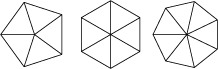
\includegraphics[scale=0.8]{../source/figs/pies.pdf}}
\caption{Turtle pies.}
\label{fig.pies}
\end{figure}


\begin{exercise}
\index{pie}

Write an appropriately general set of functions that
can draw shapes as in Figure~\ref{fig.pies}.

Solution: \url{http://thinkpython2.com/code/pie.py}.

\end{exercise}

\begin{exercise}
\index{alphabet}
\index{turtle typewriter}
\index{typewriter, turtle}

The letters of the alphabet can be constructed from a moderate number
of basic elements, like vertical and horizontal lines and a few
curves.  Design an alphabet that can be drawn with a minimal
number of basic elements and then write functions that draw the letters.

You should write one function for each letter, with names
\verb"draw_a", \verb"draw_b", etc., and put your functions
in a file named {\tt letters.py}.  You can download a
``turtle typewriter'' from \url{http://thinkpython2.com/code/typewriter.py}
to help you test your code.

You can get a solution from \url{http://thinkpython2.com/code/letters.py};
it also requires
\url{http://thinkpython2.com/code/polygon.py}.

\end{exercise}

\begin{exercise}

Read about spirals at \url{http://en.wikipedia.org/wiki/Spiral}; then
write a program that draws an Archimedian spiral (or one of the other
kinds).  Solution: \url{http://thinkpython2.com/code/spiral.py}.
\index{spiral}
\index{Archimedian spiral}

\end{exercise}


\chapter{Conditionals and recursion}

The main topic of this chapter is the {\tt if} statement, which
executes different code depending on the state of the program.
But first I want to introduce two new operators: floor division
and modulus.


\section{Floor division and modulus}

The {\bf floor division} operator, \verb"//", divides
two numbers and rounds down to an integer.  For example, suppose the
run time of a movie is 105 minutes.  You might want to know how
long that is in hours.  Conventional division
returns a floating-point number:

\begin{verbatim}
>>> minutes = 105
>>> minutes / 60
1.75
\end{verbatim}

But we don't normally write hours with decimal points.  Floor
division returns the integer number of hours, dropping the
fraction part:

\begin{verbatim}
>>> minutes = 105
>>> hours = minutes // 60
>>> hours
1
\end{verbatim}

To get the remainder, you could subtract off one hour in minutes:

\begin{verbatim}
>>> remainder = minutes - hours * 60
>>> remainder
45
\end{verbatim}

\index{floor division}
\index{floating-point division}
\index{division!floor}
\index{division!floating-point}
\index{modulus operator}
\index{operator!modulus}

An alternative is to use the {\bf modulus operator}, \verb"%", which
divides two numbers and returns the remainder.

\begin{verbatim}
>>> remainder = minutes % 60
>>> remainder
45
\end{verbatim}
%
The modulus operator is more useful than it seems.  For
example, you can check whether one number is divisible by another---if
{\tt x \% y} is zero, then {\tt x} is divisible by {\tt y}.
\index{divisibility}

Also, you can extract the right-most digit
or digits from a number.  For example, {\tt x \% 10} yields the
right-most digit of {\tt x} (in base 10).  Similarly {\tt x \% 100}
yields the last two digits.

If you are using Python 2, division works differently.  The
division operator, \verb"/", performs floor division if both
operands are integers, and floating-point division if either
operand is a {\tt float}.
\index{Python 2}


\section{Boolean expressions}
\index{boolean expression}
\index{expression!boolean}
\index{logical operator}
\index{operator!logical}

A {\bf boolean expression} is an expression that is either true
or false.  The following examples use the
operator {\tt ==}, which compares two operands and produces
{\tt True} if they are equal and {\tt False} otherwise:

\begin{verbatim}
>>> 5 == 5
True
>>> 5 == 6
False
\end{verbatim}
%
{\tt True} and {\tt False} are special
values that belong to the type {\tt bool}; they are not strings:
\index{True special value}
\index{False special value}
\index{special value!True}
\index{special value!False}
\index{bool type}
\index{type!bool}

\begin{verbatim}
>>> type(True)
<class 'bool'>
>>> type(False)
<class 'bool'>
\end{verbatim}
%
The {\tt ==} operator is one of the {\bf relational operators}; the
others are:

\begin{verbatim}
      x != y               # x is not equal to y
      x > y                # x is greater than y
      x < y                # x is less than y
      x >= y               # x is greater than or equal to y
      x <= y               # x is less than or equal to y
\end{verbatim}
%
Although these operations are probably familiar to you, the Python
symbols are different from the mathematical symbols.  A common error
is to use a single equal sign ({\tt =}) instead of a double equal sign
({\tt ==}).  Remember that {\tt =} is an assignment operator and
{\tt ==} is a relational operator.   There is no such thing as
{\tt =<} or {\tt =>}.
\index{relational operator}
\index{operator!relational}


\section {Logical operators}
\index{logical operator}
\index{operator!logical}

There are three {\bf logical operators}: {\tt and}, {\tt
or}, and {\tt not}.  The semantics (meaning) of these operators is
similar to their meaning in English.  For example,
{\tt x > 0 and x < 10} is true only if {\tt x} is greater than 0
{\em and} less than 10.
\index{and operator}
\index{or operator}
\index{not operator}
\index{operator!and}
\index{operator!or}
\index{operator!not}

{\tt n\%2 == 0 or n\%3 == 0} is true if {\em either or both} of the
conditions is true, that is, if the number is divisible by 2 {\em or}
3.

Finally, the {\tt not} operator negates a boolean
expression, so {\tt not (x > y)} is true if {\tt x > y} is false,
that is, if {\tt x} is less than or equal to {\tt y}.

Strictly speaking, the operands of the logical operators should be
boolean expressions, but Python is not very strict.
Any nonzero number is interpreted as {\tt True}:

\begin{verbatim}
>>> 42 and True
True
\end{verbatim}
%
This flexibility can be useful, but there are some subtleties to
it that might be confusing.  You might want to avoid it (unless
you know what you are doing).


\section{Conditional execution}
\label{conditional.execution}

\index{conditional statement}
\index{statement!conditional}
\index{if statement}
\index{statement!if}
\index{conditional execution}
In order to write useful programs, we almost always need the ability
to check conditions and change the behavior of the program
accordingly.  {\bf Conditional statements} give us this ability.  The
simplest form is the {\tt if} statement:

\begin{verbatim}
if x > 0:
    print('x is positive')
\end{verbatim}
%
The boolean expression after {\tt if} is
called the {\bf condition}.  If it is true, the indented
statement runs.  If not, nothing happens.
\index{condition}
\index{compound statement}
\index{statement!compound}

{\tt if} statements have the same structure as function definitions:
a header followed by an indented body.  Statements like this are
called {\bf compound statements}.

There is no limit on the number of statements that can appear in
the body, but there has to be at least one.
Occasionally, it is useful to have a body with no statements (usually
as a place keeper for code you haven't written yet).  In that
case, you can use the {\tt pass} statement, which does nothing.
\index{pass statement}
\index{statement!pass}

\begin{verbatim}
if x < 0:
    pass          # TODO: need to handle negative values!
\end{verbatim}
%

\section{Alternative execution}
\label{alternative.execution}
\index{alternative execution}
\index{else keyword}
\index{keyword!else}

A second form of the {\tt if} statement is ``alternative execution'',
in which there are two possibilities and the condition determines
which one runs.  The syntax looks like this:

\begin{verbatim}
if x % 2 == 0:
    print('x is even')
else:
    print('x is odd')
\end{verbatim}
%
If the remainder when {\tt x} is divided by 2 is 0, then we know that
{\tt x} is even, and the program displays an appropriate message.  If
the condition is false, the second set of statements runs.
Since the condition must be true or false, exactly one of the
alternatives will run.  The alternatives are called {\bf
  branches}, because they are branches in the flow of execution.
\index{branch}



\section{Chained conditionals}
\index{chained conditional}
\index{conditional!chained}

Sometimes there are more than two possibilities and we need more than
two branches.  One way to express a computation like that is a {\bf
chained conditional}:

\begin{verbatim}
if x < y:
    print('x is less than y')
elif x > y:
    print('x is greater than y')
else:
    print('x and y are equal')
\end{verbatim}
%
{\tt elif} is an abbreviation of ``else if''.  Again, exactly one
branch will run.  There is no limit on the number of {\tt
elif} statements.  If there is an {\tt else} clause, it has to be
at the end, but there doesn't have to be one.
\index{elif keyword}
\index{keyword!elif}

\begin{verbatim}
if choice == 'a':
    draw_a()
elif choice == 'b':
    draw_b()
elif choice == 'c':
    draw_c()
\end{verbatim}
%
Each condition is checked in order.  If the first is false,
the next is checked, and so on.  If one of them is
true, the corresponding branch runs and the statement
ends.  Even if more than one condition is true, only the
first true branch runs.


\section{Nested conditionals}
\index{nested conditional}
\index{conditional!nested}

One conditional can also be nested within another.  We could have
written the example in the previous section like this:

\begin{verbatim}
if x == y:
    print('x and y are equal')
else:
    if x < y:
        print('x is less than y')
    else:
        print('x is greater than y')
\end{verbatim}
%
The outer conditional contains two branches.  The
first branch contains a simple statement.  The second branch
contains another {\tt if} statement, which has two branches of its
own.  Those two branches are both simple statements,
although they could have been conditional statements as well.

Although the indentation of the statements makes the structure
apparent, {\bf nested conditionals} become difficult to read very
quickly.  It is a good idea to avoid them when you can.

Logical operators often provide a way to simplify nested conditional
statements.  For example, we can rewrite the following code using a
single conditional:

\begin{verbatim}
if 0 < x:
    if x < 10:
        print('x is a positive single-digit number.')
\end{verbatim}
%
The {\tt print} statement runs only if we make it past both
conditionals, so we can get the same effect with the {\tt and} operator:

\begin{verbatim}
if 0 < x and x < 10:
    print('x is a positive single-digit number.')
\end{verbatim}

For this kind of condition, Python provides a more concise option:

\begin{verbatim}
if 0 < x < 10:
    print('x is a positive single-digit number.')
\end{verbatim}


\section{Recursion}
\label{recursion}
\index{recursion}

It is legal for one function to call another;
it is also legal for a function to call itself.  It may not be obvious
why that is a good thing, but it turns out to be one of the most
magical things a program can do.
For example, look at the following function:

\begin{verbatim}
def countdown(n):
    if n <= 0:
        print('Blastoff!')
    else:
        print(n)
        countdown(n-1)
\end{verbatim}
%
If {\tt n} is 0 or negative, it outputs the word, ``Blastoff!''
Otherwise, it outputs {\tt n} and then calls a function named {\tt
countdown}---itself---passing {\tt n-1} as an argument.

What happens if we call this function like this?

\begin{verbatim}
>>> countdown(3)
\end{verbatim}
%
The execution of {\tt countdown} begins with {\tt n=3}, and since
{\tt n} is greater than 0, it outputs the value 3, and then calls itself...

\begin{quote}
The execution of {\tt countdown} begins with {\tt n=2}, and since
{\tt n} is greater than 0, it outputs the value 2, and then calls itself...

\begin{quote}
The execution of {\tt countdown} begins with {\tt n=1}, and since
{\tt n} is greater than 0, it outputs the value 1, and then calls itself...

\begin{quote}
The execution of {\tt countdown} begins with {\tt n=0}, and since {\tt
n} is not greater than 0, it outputs the word, ``Blastoff!'' and then
returns.
\end{quote}

The {\tt countdown} that got {\tt n=1} returns.
\end{quote}

The {\tt countdown} that got {\tt n=2} returns.
\end{quote}

The {\tt countdown} that got {\tt n=3} returns.

And then you're back in \verb"__main__".  So, the
total output looks like this:

\begin{verbatim}
3
2
1
Blastoff!
\end{verbatim}
%
A function that calls itself is {\bf recursive}; the process of
executing it is called {\bf recursion}.
\index{recursion}
\index{function!recursive}

As another example, we can write a function that prints a
string {\tt n} times.

\begin{verbatim}
def print_n(s, n):
    if n <= 0:
        return
    print(s)
    print_n(s, n-1)
\end{verbatim}
%
If {\tt n <= 0} the {\bf return statement} exits the function.  The
flow of execution immediately returns to the caller, and the remaining
lines of the function don't run.
\index{return statement}
\index{statement!return}

The rest of the function is similar to {\tt countdown}: it displays
{\tt s} and then calls itself to display {\tt s} $n-1$ additional
times.  So the number of lines of output is {\tt 1 + (n - 1)}, which
adds up to {\tt n}.

For simple examples like this, it is probably easier to use a {\tt
for} loop.  But we will see examples later that are hard to write
with a {\tt for} loop and easy to write with recursion, so it is
good to start early.
\index{for loop}
\index{loop!for}


\section{Stack diagrams for recursive functions}
\label{recursive.stack}
\index{stack diagram}
\index{function frame}
\index{frame}

In Section~\ref{stackdiagram}, we used a stack diagram to represent
the state of a program during a function call.  The same kind of
diagram can help interpret a recursive function.

Every time a function gets called, Python creates a
frame to contain the function's local variables and parameters.
For a recursive function, there might be more than one frame on the
stack at the same time.

Figure~\ref{fig.stack2} shows a stack diagram for {\tt countdown} called with
{\tt n = 3}.

\begin{figure}
\centerline
{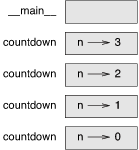
\includegraphics[scale=0.8]{../source/figs/stack2.pdf}}
\caption{Stack diagram.}
\label{fig.stack2}
\end{figure}


As usual, the top of the stack is the frame for \verb"__main__".
It is empty because we did not create any variables in
\verb"__main__" or pass any arguments to it.
\index{base case}
\index{recursion!base case}

The four {\tt countdown} frames have different values for the
parameter {\tt n}.  The bottom of the stack, where {\tt n=0}, is
called the {\bf base case}.  It does not make a recursive call, so
there are no more frames.

As an exercise, draw a stack diagram for \verb"print_n" called with
\verb"s = 'Hello'" and {\tt n=2}.
Then write a function called \verb"do_n" that takes a function
object and a number, {\tt n}, as arguments, and that calls
the given function {\tt n} times.


\section{Infinite recursion}
\index{infinite recursion}
\index{recursion!infinite}
\index{runtime error}
\index{error!runtime}
\index{traceback}

If a recursion never reaches a base case, it goes on making
recursive calls forever, and the program never terminates.  This is
known as {\bf infinite recursion}, and it is generally not
a good idea.  Here is a minimal program with an infinite recursion:

\begin{verbatim}
def recurse():
    recurse()
\end{verbatim}
%
In most programming environments, a program with infinite recursion
does not really run forever.  Python reports an error
message when the maximum recursion depth is reached:
\index{exception!RuntimeError}
\index{RuntimeError}

\begin{verbatim}
  File "<stdin>", line 2, in recurse
  File "<stdin>", line 2, in recurse
  File "<stdin>", line 2, in recurse
                  .
                  .
                  .
  File "<stdin>", line 2, in recurse
RuntimeError: Maximum recursion depth exceeded
\end{verbatim}
%
This traceback is a little bigger than the one we saw in the
previous chapter.  When the error occurs, there are 1000
{\tt recurse} frames on the stack!

If you write encounter an infinite recursion by accident, review
your function to confirm that there is a base case that does not
make a recursive call.  And if there is a base case, check whether
you are guaranteed to reach it.


\section{Keyboard input}
\index{keyboard input}

The programs we have written so far accept no input from the user.
They just do the same thing every time.

Python provides a built-in function called {\tt input} that
stops the program and
waits for the user to type something.  When the user presses {\sf
  Return} or {\sf Enter}, the program resumes and \verb"input"
returns what the user typed as a string.  In Python 2, the same
function is called \verb"raw_input".
\index{Python 2}
\index{input function}
\index{function!input}

\begin{verbatim}
>>> text = input()
What are you waiting for?
>>> text
What are you waiting for?
\end{verbatim}
%
Before getting input from the user, it is a good idea to print a
prompt telling the user what to type.  \verb"input" can take a
prompt as an argument:
\index{prompt}

\begin{verbatim}
>>> name = input('What...is your name?\n')
What...is your name?
Arthur, King of the Britons!
>>> name
Arthur, King of the Britons!
\end{verbatim}
%
The sequence \verb"\n" at the end of the prompt represents a {\bf
  newline}, which is a special character that causes a line break.
That's why the user's input appears below the prompt.  \index{newline}

If you expect the user to type an integer, you can try to convert
the return value to {\tt int}:

\begin{verbatim}
>>> prompt = 'What...is the airspeed velocity of an unladen swallow?\n'
>>> speed = input(prompt)
What...is the airspeed velocity of an unladen swallow?
42
>>> int(speed)
42
\end{verbatim}
%
But if the user types something other than a string of digits,
you get an error:

\begin{verbatim}
>>> speed = input(prompt)
What...is the airspeed velocity of an unladen swallow?
What do you mean, an African or a European swallow?
>>> int(speed)
ValueError: invalid literal for int() with base 10
\end{verbatim}
%
We will see how to handle this kind of error later.
\index{ValueError}
\index{exception!ValueError}


\section{Debugging}
\label{whitespace}
\index{debugging}
\index{traceback}

When a syntax or runtime error occurs, the error message contains
a lot of information, but it can be overwhelming.  The most
useful parts are usually:

\begin{itemize}

\item What kind of error it was, and

\item Where it occurred.

\end{itemize}

Syntax errors are usually easy to find, but there are a few
gotchas.  Whitespace errors can be tricky because spaces and
tabs are invisible and we are used to ignoring them.
\index{whitespace}

\begin{verbatim}
>>> x = 5
>>>  y = 6
  File "<stdin>", line 1
    y = 6
    ^
IndentationError: unexpected indent
\end{verbatim}
%
In this example, the problem is that the second line is indented by
one space.  But the error message points to {\tt y}, which is
misleading.  In general, error messages indicate where the problem was
discovered, but the actual error might be earlier in the code,
sometimes on a previous line.
\index{error!runtime}
\index{runtime error}

The same is true of runtime errors.  Suppose you are trying
to compute a signal-to-noise ratio in decibels.  The formula
is $SNR_{db} = 10 \log_{10} (P_{signal} / P_{noise})$.  In Python,
you might write something like this:

\begin{verbatim}
import math
signal_power = 9
noise_power = 10
ratio = signal_power // noise_power
decibels = 10 * math.log10(ratio)
print(decibels)
\end{verbatim}
%
When you run this program, you get an exception:
%
\index{exception!OverflowError}
\index{OverflowError}

\begin{verbatim}
Traceback (most recent call last):
  File "snr.py", line 5, in ?
    decibels = 10 * math.log10(ratio)
ValueError: math domain error
\end{verbatim}
%
The error message indicates line 5, but there is nothing
wrong with that line.  To find the real error, it might be
useful to print the value of {\tt ratio}, which turns out to
be 0.  The problem is in line 4, which uses floor division
instead of floating-point division.
\index{floor division}
\index{division!floor}

You should take the time to read error messages carefully, but don't
assume that everything they say is correct.


\section{Glossary}

\begin{description}

\item[floor division:] An operator, denoted {\tt //}, that divides two
  numbers and rounds down (toward zero) to an integer.
  \index{floor division}
  \index{division!floor}

\item[modulus operator:]  An operator, denoted with a percent sign
({\tt \%}), that works on integers and returns the remainder when one
number is divided by another.
\index{modulus operator}
\index{operator!modulus}

\item[boolean expression:]  An expression whose value is either
{\tt True} or {\tt False}.
\index{boolean expression}
\index{expression!boolean}

\item[relational operator:] One of the operators that compares
its operands: {\tt ==}, {\tt !=}, {\tt >}, {\tt <}, {\tt >=}, and {\tt <=}.

\item[logical operator:] One of the operators that combines boolean
expressions: {\tt and}, {\tt or}, and {\tt not}.

\item[conditional statement:]  A statement that controls the flow of
execution depending on some condition.
\index{conditional statement}
\index{statement!conditional}

\item[condition:] The boolean expression in a conditional statement
that determines which branch runs.
\index{condition}

\item[compound statement:]  A statement that consists of a header
and a body.  The header ends with a colon (:).  The body is indented
relative to the header.
\index{compound statement}

\item[branch:] One of the alternative sequences of statements in
a conditional statement.
\index{branch}

\item[chained conditional:]  A conditional statement with a series
of alternative branches.
\index{chained conditional}
\index{conditional!chained}

\item[nested conditional:]  A conditional statement that appears
in one of the branches of another conditional statement.
\index{nested conditional}
\index{conditional!nested}

\item[return statement:] A statement that causes a function to
end immediately and return to the caller.

\item[recursion:]  The process of calling the function that is
currently executing.
\index{recursion}

\item[base case:]  A conditional branch in a
recursive function that does not make a recursive call.
\index{base case}

\item[infinite recursion:]  A recursion that doesn't have a
base case, or never reaches it.  Eventually, an infinite recursion
causes a runtime error.
\index{infinite recursion}

\end{description}

\section{Exercises}

\begin{exercise}

The {\tt time} module provides a function, also named {\tt time}, that
returns the current Greenwich Mean Time in ``the epoch'', which is
an arbitrary time used as a reference point.  On UNIX systems, the
epoch is 1 January 1970.

\begin{verbatim}
>>> import time
>>> time.time()
1437746094.5735958
\end{verbatim}

Write a script that reads the current time and converts it to
a time of day in hours, minutes, and seconds, plus the number of
days since the epoch.

\end{exercise}


\begin{exercise}
\index{Fermat's Last Theorem}

Fermat's Last Theorem says that there are no positive integers
$a$, $b$, and $c$ such that

\[ a^n + b^n = c^n \]
%
for any values of $n$ greater than 2.

\begin{enumerate}

\item Write a function named \verb"check_fermat" that takes four
parameters---{\tt a}, {\tt b}, {\tt c} and {\tt n}---and
checks to see if Fermat's theorem holds.  If
$n$ is greater than 2 and

\[a^n + b^n = c^n \]
%
the program should print, ``Holy smokes, Fermat was wrong!''
Otherwise the program should print, ``No, that doesn't work.''

\item Write a function that prompts the user to input values
for {\tt a}, {\tt b}, {\tt c} and {\tt n}, converts them to
integers, and uses \verb"check_fermat" to check whether they
violate Fermat's theorem.

\end{enumerate}

\end{exercise}


\begin{exercise}
\index{triangle}

If you are given three sticks, you may or may not be able to arrange
them in a triangle.  For example, if one of the sticks is 12 inches
long and the other two are one inch long, you will
not be able to get the short sticks to meet in the middle.  For any
three lengths, there is a simple test to see if it is possible to form
a triangle:

\begin{quotation}
If any of the three lengths is greater than the sum of the other
  two, then you cannot form a triangle.  Otherwise, you
  can.  (If the sum of two lengths equals the third, they form
    what is called a ``degenerate'' triangle.)
\end{quotation}

\begin{enumerate}

\item Write a function named \verb"is_triangle" that takes three
  integers as arguments, and that prints either ``Yes'' or ``No'', depending
  on whether you can or cannot form a triangle from sticks with the
  given lengths.

\item Write a function that prompts the user to input three stick
  lengths, converts them to integers, and uses \verb"is_triangle" to
  check whether sticks with the given lengths can form a triangle.

\end{enumerate}

\end{exercise}

\begin{exercise}
What is the output of the following program?
Draw a stack diagram that shows the state of the program
when it prints the result.

\begin{verbatim}
def recurse(n, s):
    if n == 0:
        print(s)
    else:
        recurse(n-1, n+s)

recurse(3, 0)
\end{verbatim}

\begin{enumerate}

\item What would happen if you called this function like this: {\tt
  recurse(-1, 0)}?

\item Write a docstring that explains everything someone would need to
  know in order to use this function (and nothing else).

\end{enumerate}

\end{exercise}


The following exercises use the {\tt turtle} module, described in
Chapter~\ref{turtlechap}:
\index{TurtleWorld}

\begin{exercise}

Read the following function and see if you can figure out
what it does.  Then run it (see the examples in Chapter~\ref{turtlechap}).

\begin{verbatim}
def draw(t, length, n):
    if n == 0:
        return
    angle = 50
    t.fd(length*n)
    t.lt(angle)
    draw(t, length, n-1)
    t.rt(2*angle)
    draw(t, length, n-1)
    t.lt(angle)
    t.bk(length*n)
\end{verbatim}

\end{exercise}


\begin{figure}
\centerline
{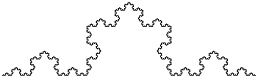
\includegraphics[scale=0.8]{../source/figs/koch.pdf}}
\caption{A Koch curve.}
\label{fig.koch}
\end{figure}

\begin{exercise}
\index{Koch curve}

The Koch curve is a fractal that looks something like
Figure~\ref{fig.koch}.  To draw a Koch curve with length $x$, all you
have to do is

\begin{enumerate}

\item Draw a Koch curve with length $x/3$.

\item Turn left 60 degrees.

\item Draw a Koch curve with length $x/3$.

\item Turn right 120 degrees.

\item Draw a Koch curve with length $x/3$.

\item Turn left 60 degrees.

\item Draw a Koch curve with length $x/3$.

\end{enumerate}

The exception is if $x$ is less than 3: in that case,
you can just draw a straight line with length $x$.

\begin{enumerate}

\item Write a function called {\tt koch} that takes a turtle and
a length as parameters, and that uses the turtle to draw a Koch
curve with the given length.

\item Write a function called {\tt snowflake} that draws three
Koch curves to make the outline of a snowflake.

Solution: \url{http://thinkpython2.com/code/koch.py}.

\item The Koch curve can be generalized in several ways.  See
\url{http://en.wikipedia.org/wiki/Koch_snowflake} for examples and
implement your favorite.

\end{enumerate}
\end{exercise}


\chapter{Fruitful functions}
\label{fruitchap}

Many of the Python functions we have used, such as the math
functions, produce return values.  But the functions we've written
are all void: they have an effect, like printing a value
or moving a turtle, but they don't have a return value.  In
this chapter you will learn to write fruitful functions.


\section{Return values}
\index{return value}

Calling the function generates a return
value, which we usually assign to a variable or use as part of an
expression.

\begin{verbatim}
e = math.exp(1.0)
height = radius * math.sin(radians)
\end{verbatim}
%
The functions we have written so far are void.  Speaking casually,
they have no return value; more precisely,
their return value is {\tt None}.

In this chapter, we are (finally) going to write fruitful functions.
The first example is {\tt area}, which returns the area of a circle
with the given radius:

\begin{verbatim}
def area(radius):
    a = math.pi * radius**2
    return a
\end{verbatim}
%
We have seen the {\tt return} statement before, but in a fruitful
function the {\tt return} statement includes
an expression.  This statement means: ``Return immediately from
this function and use the following expression as a return value.''
The expression can be arbitrarily complicated, so we could
have written this function more concisely:
\index{return statement}
\index{statement!return}

\begin{verbatim}
def area(radius):
    return math.pi * radius**2
\end{verbatim}
%
On the other hand, {\bf temporary variables} like {\tt a} can make
debugging easier.
\index{temporary variable}
\index{variable!temporary}

Sometimes it is useful to have multiple return statements, one in each
branch of a conditional:

\begin{verbatim}
def absolute_value(x):
    if x < 0:
        return -x
    else:
        return x
\end{verbatim}
%
Since these {\tt return} statements are in an alternative conditional,
only one runs.

As soon as a return statement runs, the function
terminates without executing any subsequent statements.
Code that appears after a {\tt return} statement, or any other place
the flow of execution can never reach, is called {\bf dead code}.
\index{dead code}

In a fruitful function, it is a good idea to ensure
that every possible path through the program hits a
{\tt return} statement.  For example:

\begin{verbatim}
def absolute_value(x):
    if x < 0:
        return -x
    if x > 0:
        return x
\end{verbatim}
%
This function is incorrect because if {\tt x} happens to be 0,
neither condition is true, and the function ends without hitting a
{\tt return} statement.  If the flow of execution gets to the end
of a function, the return value is {\tt None}, which is not
the absolute value of 0.
\index{None special value}
\index{special value!None}

\begin{verbatim}
>>> absolute_value(0)
None
\end{verbatim}
%
By the way, Python provides a built-in function called
{\tt abs} that computes absolute values.
\index{abs function}
\index{function!abs}

As an exercise, write a {\tt compare} function
takes two values, {\tt x} and {\tt y}, and returns {\tt 1} if {\tt x > y},
{\tt 0} if {\tt x == y}, and {\tt -1} if {\tt x < y}.
\index{compare function}
\index{function!compare}


\section{Incremental development}
\label{incremental.development}
\index{development plan!incremental}

As you write larger functions, you might find yourself
spending more time debugging.

To deal with increasingly complex programs,
you might want to try a process called
{\bf incremental development}.  The goal of incremental development
is to avoid long debugging sessions by adding and testing only
a small amount of code at a time.
\index{testing!incremental development}
\index{Pythagorean theorem}

As an example, suppose you want to find the distance between two
points, given by the coordinates $(x_1, y_1)$ and $(x_2, y_2)$.
By the Pythagorean theorem, the distance is:

\begin{displaymath}
\mathrm{distance} = \sqrt{(x_2 - x_1)^2 + (y_2 - y_1)^2}
\end{displaymath}
%
The first step is to consider what a {\tt distance} function should
look like in Python.  In other words, what are the inputs (parameters)
and what is the output (return value)?

In this case, the inputs are two points, which you can represent
using four numbers.  The return value is the distance represented by
a floating-point value.

Immediately you can write an outline of the function:

\begin{verbatim}
def distance(x1, y1, x2, y2):
    return 0.0
\end{verbatim}
%
Obviously, this version doesn't compute distances; it always returns
zero.  But it is syntactically correct, and it runs, which means that
you can test it before you make it more complicated.

To test the new function, call it with sample arguments:

\begin{verbatim}
>>> distance(1, 2, 4, 6)
0.0
\end{verbatim}
%
I chose these values so that the horizontal distance is 3 and the
vertical distance is 4; that way, the result is 5, the hypotenuse
of a 3-4-5 triangle. When testing a function, it is
useful to know the right answer.
\index{testing!knowing the answer}

At this point we have confirmed that the function is syntactically
correct, and we can start adding code to the body.
A reasonable next step is to find the differences
$x_2 - x_1$ and $y_2 - y_1$.  The next version stores those values in
temporary variables and prints them.

\begin{verbatim}
def distance(x1, y1, x2, y2):
    dx = x2 - x1
    dy = y2 - y1
    print('dx is', dx)
    print('dy is', dy)
    return 0.0
\end{verbatim}
%
If the function is working, it should display \verb"dx is 3" and
\verb"dy is 4".  If so, we know that the function is getting the right
arguments and performing the first computation correctly.  If not,
there are only a few lines to check.

Next we compute the sum of squares of {\tt dx} and {\tt dy}:

\begin{verbatim}
def distance(x1, y1, x2, y2):
    dx = x2 - x1
    dy = y2 - y1
    dsquared = dx**2 + dy**2
    print('dsquared is: ', dsquared)
    return 0.0
\end{verbatim}
%
Again, you would run the program at this stage and check the output
(which should be 25).
Finally, you can use {\tt math.sqrt} to compute and return the result:
\index{sqrt}
\index{function!sqrt}

\begin{verbatim}
def distance(x1, y1, x2, y2):
    dx = x2 - x1
    dy = y2 - y1
    dsquared = dx**2 + dy**2
    result = math.sqrt(dsquared)
    return result
\end{verbatim}
%
If that works correctly, you are done.  Otherwise, you might
want to print the value of {\tt result} before the return
statement.

The final version of the function doesn't display anything when it
runs; it only returns a value.  The {\tt print} statements we wrote
are useful for debugging, but once you get the function working, you
should remove them.  Code like that is called {\bf scaffolding}
because it is helpful for building the program but is not part of the
final product.
\index{scaffolding}

When you start out, you should add only a line or two of code at a
time.  As you gain more experience, you might find yourself writing
and debugging bigger chunks.  Either way, incremental development
can save you a lot of debugging time.

The key aspects of the process are:

\begin{enumerate}

\item Start with a working program and make small incremental changes.
At any point, if there is an error, you should have a good idea
where it is.

\item Use variables to hold intermediate values so you can
display and check them.

\item Once the program is working, you might want to remove some of
the scaffolding or consolidate multiple statements into compound
expressions, but only if it does not make the program difficult to
read.

\end{enumerate}

As an exercise, use incremental development to write a function
called {\tt hypotenuse} that returns the length of the hypotenuse of a
right triangle given the lengths of the other two legs as arguments.
Record each stage of the development process as you go.
\index{hypotenuse}



\section{Composition}
\index{composition}
\index{function composition}

As you should expect by now, you can call one function from within
another.  As an example, we'll write a function that takes two points,
the center of the circle and a point on the perimeter, and computes
the area of the circle.

Assume that the center point is stored in the variables {\tt xc} and
{\tt yc}, and the perimeter point is in {\tt xp} and {\tt yp}. The
first step is to find the radius of the circle, which is the distance
between the two points.  We just wrote a function, {\tt
distance}, that does that:

\begin{verbatim}
radius = distance(xc, yc, xp, yp)
\end{verbatim}
%
The next step is to find the area of a circle with that radius;
we just wrote that, too:

\begin{verbatim}
result = area(radius)
\end{verbatim}
%
Encapsulating these steps in a function, we get:
\index{encapsulation}

\begin{verbatim}
def circle_area(xc, yc, xp, yp):
    radius = distance(xc, yc, xp, yp)
    result = area(radius)
    return result
\end{verbatim}
%
The temporary variables {\tt radius} and {\tt result} are useful for
development and debugging, but once the program is working, we can
make it more concise by composing the function calls:

\begin{verbatim}
def circle_area(xc, yc, xp, yp):
    return area(distance(xc, yc, xp, yp))
\end{verbatim}
%

\section{Boolean functions}
\label{boolean}

Functions can return booleans, which is often convenient for hiding
complicated tests inside functions.  \index{boolean function}
For example:

\begin{verbatim}
def is_divisible(x, y):
    if x % y == 0:
        return True
    else:
        return False
\end{verbatim}
%
It is common to give boolean functions names that sound like yes/no
questions; \verb"is_divisible" returns either {\tt True} or {\tt False}
to indicate whether {\tt x} is divisible by {\tt y}.

Here is an example:

\begin{verbatim}
>>> is_divisible(6, 4)
False
>>> is_divisible(6, 3)
True
\end{verbatim}
%
The result of the {\tt ==} operator is a boolean, so we can write the
function more concisely by returning it directly:

\begin{verbatim}
def is_divisible(x, y):
    return x % y == 0
\end{verbatim}
%
Boolean functions are often used in conditional statements:
\index{conditional statement}
\index{statement!conditional}

\begin{verbatim}
if is_divisible(x, y):
    print('x is divisible by y')
\end{verbatim}
%
It might be tempting to write something like:

\begin{verbatim}
if is_divisible(x, y) == True:
    print('x is divisible by y'
\end{verbatim}
%
But the extra comparison is unnecessary.

As an exercise, write a function \verb"is_between(x, y, z)" that
returns {\tt True} if $x \le y \le z$ or {\tt False} otherwise.


\section{More recursion}
\label{more.recursion}
\index{recursion}
\index{Turing complete language}
\index{language!Turing complete}
\index{Turing, Alan}
\index{Turing Thesis}

We have only covered a small subset of Python, but you might
be interested to know that this subset is a {\em complete}
programming language, which means that anything that can be
computed can be expressed in this language.  Any program ever written
could be rewritten using only the language features you have learned
so far (actually, you would need a few commands to control devices
like the mouse, disks, etc., but that's all).

Proving that claim is a nontrivial exercise first accomplished by Alan
Turing, one of the first computer scientists (some would argue that he
was a mathematician, but a lot of early computer scientists started as
mathematicians).  Accordingly, it is known as the Turing Thesis.
For a more complete (and accurate) discussion of the Turing Thesis,
I recommend Michael Sipser's book {\em Introduction to the
Theory of Computation}.

To give you an idea of what you can do with the tools you have learned
so far, we'll evaluate a few recursively defined mathematical
functions.  A recursive definition is similar to a circular
definition, in the sense that the definition contains a reference to
the thing being defined.  A truly circular definition is not very
useful:

\begin{description}

\item[vorpal:] An adjective used to describe something that is vorpal.
\index{vorpal}
\index{circular definition}
\index{definition!circular}

\end{description}

If you saw that definition in the dictionary, you might be annoyed. On
the other hand, if you looked up the definition of the factorial
function, denoted with the symbol $!$, you might get something like
this:
%
\begin{eqnarray*}
&&  0! = 1 \\
&&  n! = n (n-1)!
\end{eqnarray*}
%
This definition says that the factorial of 0 is 1, and the factorial
of any other value, $n$, is $n$ multiplied by the factorial of $n-1$.

So $3!$ is 3 times $2!$, which is 2 times $1!$, which is 1 times
$0!$. Putting it all together, $3!$ equals 3 times 2 times 1 times 1,
which is 6.
\index{factorial function}
\index{function!factorial}
\index{recursive definition}

If you can write a recursive definition of something, you can
write a Python program to evaluate it. The first step is to decide
what the parameters should be.  In this case it should be clear
that {\tt factorial} takes an integer:

\begin{verbatim}
def factorial(n):
\end{verbatim}
%
If the argument happens to be 0, all we have to do is return 1:

\begin{verbatim}
def factorial(n):
    if n == 0:
        return 1
\end{verbatim}
%
Otherwise, and this is the interesting part, we have to make a
recursive call to find the factorial of $n-1$ and then multiply it by
$n$:

\begin{verbatim}
def factorial(n):
    if n == 0:
        return 1
    else:
        recurse = factorial(n-1)
        result = n * recurse
        return result
\end{verbatim}
%
The flow of execution for this program is similar to the flow of {\tt
countdown} in Section~\ref{recursion}.  If we call {\tt factorial}
with the value 3:

Since 3 is not 0, we take the second branch and calculate the factorial
of {\tt n-1}...

\begin{quote}
Since 2 is not 0, we take the second branch and calculate the factorial of
{\tt n-1}...


  \begin{quote}
  Since 1 is not 0, we take the second branch and calculate the factorial
  of {\tt n-1}...


    \begin{quote}
    Since 0 equals 0, we take the first branch and return 1
    without making any more recursive calls.
    \end{quote}


  The return value, 1, is multiplied by $n$, which is 1, and the
  result is returned.
  \end{quote}


The return value, 1, is multiplied by $n$, which is 2, and the
result is returned.
\end{quote}


The return value (2) is multiplied by $n$, which is 3, and the result, 6,
becomes the return value of the function call that started the whole
process.
\index{stack diagram}

Figure~\ref{fig.stack3} shows what the stack diagram looks like for
this sequence of function calls.

\begin{figure}
\centerline
{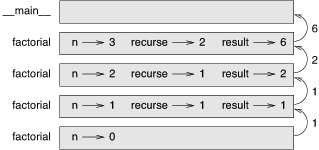
\includegraphics[scale=0.8]{../source/figs/stack3.pdf}}
\caption{Stack diagram.}
\label{fig.stack3}
\end{figure}

The return values are shown being passed back up the stack.  In each
frame, the return value is the value of {\tt result}, which is the
product of {\tt n} and {\tt recurse}.
\index{function frame}
\index{frame}

In the last frame, the local
variables {\tt recurse} and {\tt result} do not exist, because
the branch that creates them does not run.


\section{Leap of faith}
\index{recursion}
\index{leap of faith}

Following the flow of execution is one way to read programs, but
it can quickly become overwhelming.  An
alternative is what I call the ``leap of faith''.  When you come to a
function call, instead of following the flow of execution, you {\em
assume} that the function works correctly and returns the right
result.

In fact, you are already practicing this leap of faith when you use
built-in functions.  When you call {\tt math.cos} or {\tt math.exp},
you don't examine the bodies of those functions.  You just
assume that they work because the people who wrote the built-in
functions were good programmers.

The same is true when you call one of your own functions.  For
example, in Section~\ref{boolean}, we wrote a function called
\verb"is_divisible" that determines whether one number is divisible by
another.  Once we have convinced ourselves that this function is
correct---by examining the code and testing---we can use the function
without looking at the body again.
\index{testing!leap of faith}

The same is true of recursive programs.  When you get to the recursive
call, instead of following the flow of execution, you should assume
that the recursive call works (returns the correct result) and then ask
yourself, ``Assuming that I can find the factorial of $n-1$, can I
compute the factorial of $n$?''  It is clear that you
can, by multiplying by $n$.

Of course, it's a bit strange to assume that the function works
correctly when you haven't finished writing it, but that's why
it's called a leap of faith!


\section{One more example}
\label{one.more.example}

\index{fibonacci function}
\index{function!fibonacci}
After {\tt factorial}, the most common example of a recursively
defined mathematical function is {\tt fibonacci}, which has the
following definition (see
  \url{http://en.wikipedia.org/wiki/Fibonacci_number}):
%
\begin{eqnarray*}
&& \mathrm{fibonacci}(0) = 0 \\
&& \mathrm{fibonacci}(1) = 1 \\
&& \mathrm{fibonacci}(n) = \mathrm{fibonacci}(n-1) + \mathrm{fibonacci}(n-2)
\end{eqnarray*}
%
Translated into Python, it looks like this:

\begin{verbatim}
def fibonacci (n):
    if n == 0:
        return 0
    elif  n == 1:
        return 1
    else:
        return fibonacci(n-1) + fibonacci(n-2)
\end{verbatim}
%
If you try to follow the flow of execution here, even for fairly
small values of $n$, your head explodes.  But according to the
leap of faith, if you assume that the two recursive calls
work correctly, then it is clear that you get
the right result by adding them together.
\index{flow of execution}


\section{Checking types}
\label{guardian}

What happens if we call {\tt factorial} and give it 1.5 as an argument?
\index{type checking}
\index{error checking}
\index{factorial function}
\index{RuntimeError}

\begin{verbatim}
>>> factorial(1.5)
RuntimeError: Maximum recursion depth exceeded
\end{verbatim}
%
It looks like an infinite recursion.  How can that be?  The function
has a base case---when {\tt n == 0}.  But if {\tt n} is not an integer,
we can {\em miss} the base case and recurse forever.
\index{infinite recursion}
\index{recursion!infinite}

In the first recursive call, the value of {\tt n} is 0.5.
In the next, it is -0.5.  From there, it gets smaller
(more negative), but it will never be 0.

We have two choices.  We can try to generalize the {\tt factorial}
function to work with floating-point numbers, or we can make {\tt
  factorial} check the type of its argument.  The first option is
called the gamma function and it's a
little beyond the scope of this book.  So we'll go for the second.
\index{gamma function}

We can use the built-in function {\tt isinstance} to verify the type
of the argument.  While we're at it, we can also make sure the
argument is positive:
\index{isinstance function}
\index{function!isinstance}

\begin{verbatim}
def factorial (n):
    if not isinstance(n, int):
        print('Factorial is only defined for integers.')
        return None
    elif n < 0:
        print('Factorial is not defined for negative integers.')
        return None
    elif n == 0:
        return 1
    else:
        return n * factorial(n-1)
\end{verbatim}
%
The first base case handles nonintegers; the
second handles negative integers.  In both cases, the program prints
an error message and returns {\tt None} to indicate that something
went wrong:

\begin{verbatim}
>>> factorial('fred')
Factorial is only defined for integers.
None
>>> factorial(-2)
Factorial is not defined for negative integers.
None
\end{verbatim}
%
If we get past both checks, we know that $n$ is positive or
zero, so we can prove that the recursion terminates.
\index{guardian pattern}
\index{pattern!guardian}

This program demonstrates a pattern sometimes called a {\bf guardian}.
The first two conditionals act as guardians, protecting the code that
follows from values that might cause an error.  The guardians make it
possible to prove the correctness of the code.

In Section~\ref{raise} we will see a more flexible alternative to printing
an error message: raising an exception.


\section{Debugging}
\label{factdebug}

Breaking a large program into smaller functions creates natural
checkpoints for debugging.  If a function is not
working, there are three possibilities to consider:
\index{debugging}

\begin{itemize}

\item There is something wrong with the arguments the function
is getting; a precondition is violated.

\item There is something wrong with the function; a postcondition
is violated.

\item There is something wrong with the return value or the
way it is being used.

\end{itemize}

To rule out the first possibility, you can add a {\tt print} statement
at the beginning of the function and display the values of the
parameters (and maybe their types).  Or you can write code
that checks the preconditions explicitly.
\index{precondition}
\index{postcondition}

If the parameters look good, add a {\tt print} statement before each
{\tt return} statement and display the return value.  If
possible, check the result by hand.  Consider calling the
function with values that make it easy to check the result
(as in Section~\ref{incremental.development}).

If the function seems to be working, look at the function call
to make sure the return value is being used correctly (or used
at all!).
\index{flow of execution}

Adding print statements at the beginning and end of a function
can help make the flow of execution more visible.
For example, here is a version of {\tt factorial} with
print statements:

\begin{verbatim}
def factorial(n):
    space = ' ' * (4 * n)
    print(space, 'factorial', n)
    if n == 0:
        print(space, 'returning 1')
        return 1
    else:
        recurse = factorial(n-1)
        result = n * recurse
        print(space, 'returning', result)
        return result
\end{verbatim}
%
{\tt space} is a string of space characters that controls the
indentation of the output.  Here is the result of {\tt factorial(4)} :

\begin{verbatim}
                 factorial 4
             factorial 3
         factorial 2
     factorial 1
 factorial 0
 returning 1
     returning 1
         returning 2
             returning 6
                 returning 24
\end{verbatim}
%
If you are confused about the flow of execution, this kind of
output can be helpful.  It takes some time to develop effective
scaffolding, but a little bit of scaffolding can save a lot of debugging.


\section{Glossary}

\begin{description}

\item[temporary variable:]  A variable used to store an intermediate value in
a complex calculation.
\index{temporary variable}
\index{variable!temporary}

\item[dead code:]  Part of a program that can never run, often because
it appears after a {\tt return} statement.
\index{dead code}

\item[incremental development:]  A program development plan intended to
avoid debugging by adding and testing only
a small amount of code at a time.
\index{incremental development}

\item[scaffolding:]  Code that is used during program development but is
not part of the final version.
\index{scaffolding}

\item[guardian:]  A programming pattern that uses a conditional
statement to check for and handle circumstances that
might cause an error.
\index{guardian pattern}
\index{pattern!guardian}

\end{description}


\section{Exercises}

\begin{exercise}

Draw a stack diagram for the following program.  What does the program print?
\index{stack diagram}

\begin{verbatim}
def b(z):
    prod = a(z, z)
    print(z, prod)
    return prod

def a(x, y):
    x = x + 1
    return x * y

def c(x, y, z):
    total = x + y + z
    square = b(total)**2
    return square

x = 1
y = x + 1
print(c(x, y+3, x+y))
\end{verbatim}

\end{exercise}


\begin{exercise}
\label{ackermann}

The Ackermann function, $A(m, n)$, is defined:

\begin{eqnarray*}
A(m, n) = \begin{cases}
              n+1 & \mbox{if } m = 0 \\
        A(m-1, 1) & \mbox{if } m > 0 \mbox{ and } n = 0 \\
A(m-1, A(m, n-1)) & \mbox{if } m > 0 \mbox{ and } n > 0.
\end{cases}
\end{eqnarray*}
%
See \url{http://en.wikipedia.org/wiki/Ackermann_function}.
Write a function named {\tt ack} that evaluates the Ackermann function.
Use your function to evaluate {\tt ack(3, 4)}, which should be 125.
What happens for larger values of {\tt m} and {\tt n}?
Solution: \url{http://thinkpython2.com/code/ackermann.py}.
\index{Ackermann function}
\index{function!ack}

\end{exercise}


\begin{exercise}
\label{palindrome}

A palindrome is a word that is spelled the same backward and
forward, like ``noon'' and ``redivider''.  Recursively, a word
is a palindrome if the first and last letters are the same
and the middle is a palindrome.
\index{palindrome}

The following are functions that take a string argument and
return the first, last, and middle letters:

\begin{verbatim}
def first(word):
    return word[0]

def last(word):
    return word[-1]

def middle(word):
    return word[1:-1]
\end{verbatim}
%
We'll see how they work in Chapter~\ref{strings}.

\begin{enumerate}

\item Type these functions into a file named {\tt palindrome.py}
and test them out.  What happens if you call {\tt middle} with
a string with two letters?  One letter?  What about the empty
string, which is written \verb"''" and contains no letters?

\item Write a function called \verb"is_palindrome" that takes
a string argument and returns {\tt True} if it is a palindrome
and {\tt False} otherwise.  Remember that you can use the
built-in function {\tt len} to check the length of a string.

\end{enumerate}

Solution: \url{http://thinkpython2.com/code/palindrome_soln.py}.

\end{exercise}

\begin{exercise}

A number, $a$, is a power of $b$ if it is divisible by $b$
and $a/b$ is a power of $b$.  Write a function called
\verb"is_power" that takes parameters {\tt a} and {\tt b}
and returns {\tt True} if {\tt a} is a power of {\tt b}.
Note: you will have to think about the base case.

\end{exercise}


\begin{exercise}
\index{greatest common divisor (GCD)}
\index{GCD (greatest common divisor)}

The greatest common divisor (GCD) of $a$ and $b$ is the largest number
that divides both of them with no remainder.

One way to find the GCD of two numbers is based on the observation
that if $r$ is the remainder when $a$ is divided by $b$, then $gcd(a,
b) = gcd(b, r)$.  As a base case, we can use $gcd(a, 0) = a$.

Write a function called
\verb"gcd" that takes parameters {\tt a} and {\tt b}
and returns their greatest common divisor.

Credit: This exercise is based on an example from Abelson and
Sussman's {\em Structure and Interpretation of Computer Programs}.

\end{exercise}


\chapter{Iteration}

This chapter is about iteration, which is the ability to run
a block of statements repeatedly.  We saw a kind of iteration,
using recursion, in Section~\ref{recursion}.
We saw another kind, using a {\tt for} loop,
in Section~\ref{repetition}.  In this chapter we'll see yet another
kind, using a {\tt while} statement.
But first I want to say a little more about variable assignment.


\section{Reassignment}
\index{assignment}
\index{statement!assignment}
\index{reassignment}

As you may have discovered, it is legal to make more than one
assignment to the same variable.  A new assignment makes an existing
variable refer to a new value (and stop referring to the old value).

\begin{verbatim}
>>> x = 5
>>> x
5
>>> x = 7
>>> x
7
\end{verbatim}
%
The first time we display
{\tt x}, its value is 5; the second time, its
value is 7.

Figure~\ref{fig.assign2} shows what {\bf reassignment} looks
like in a state diagram. \index{state diagram} \index{diagram!state}

At this point I want to address a common source of
confusion.
Because Python uses the equal sign ({\tt =}) for assignment, it is
tempting to interpret a statement like {\tt a = b} as a
mathematical
proposition of equality; that is, the claim that {\tt a} and
{\tt b} are equal.  But this interpretation is wrong.
\index{equality and assignment}

First, equality is a symmetric relationship and assignment is not.  For
example, in mathematics, if $a=7$ then $7=a$.  But in Python, the
statement {\tt a = 7} is legal and {\tt 7 = a} is not.

Also, in mathematics, a proposition of equality is either true or
false for all time.  If $a=b$ now, then $a$ will always equal $b$.
In Python, an assignment statement can make two variables equal, but
they don't have to stay that way:

\begin{verbatim}
>>> a = 5
>>> b = a    # a and b are now equal
>>> a = 3    # a and b are no longer equal
>>> b
5
\end{verbatim}
%
The third line changes the value of {\tt a} but does not change the
value of {\tt b}, so they are no longer equal.

Reassigning variables is often useful, but you should use it
with caution.  If the values of variables change frequently, it can
make the code difficult to read and debug.

\begin{figure}
\centerline
{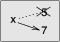
\includegraphics[scale=0.8]{../source/figs/assign2.pdf}}
\caption{State diagram.}
\label{fig.assign2}
\end{figure}



\section{Updating variables}
\label{update}

\index{update}
\index{variable!updating}

A common kind of reassignment is an {\bf update},
where the new value of the variable depends on the old.

\begin{verbatim}
>>> x = x + 1
\end{verbatim}
%
This means ``get the current value of {\tt x}, add one, and then
update {\tt x} with the new value.''

If you try to update a variable that doesn't exist, you get an
error, because Python evaluates the right side before it assigns
a value to {\tt x}:

\begin{verbatim}
>>> x = x + 1
NameError: name 'x' is not defined
\end{verbatim}
%
Before you can update a variable, you have to {\bf initialize}
it, usually with a simple assignment:
\index{initialization (before update)}

\begin{verbatim}
>>> x = 0
>>> x = x + 1
\end{verbatim}
%
Updating a variable by adding 1 is called an {\bf increment};
subtracting 1 is called a {\bf decrement}.
\index{increment}
\index{decrement}




\section{The {\tt while} statement}
\index{statement!while}
\index{while loop}
\index{loop!while}
\index{iteration}

Computers are often used to automate repetitive tasks.  Repeating
identical or similar tasks without making errors is something that
computers do well and people do poorly.  In a computer program,
repetition is also called {\bf iteration}.

We have already seen two functions, {\tt countdown} and
\verb"print_n", that iterate using recursion.  Because iteration is so
common, Python provides language features to make it easier.
One is the {\tt for} statement we saw in Section~\ref{repetition}.
We'll get back to that later.

Another is the {\tt while} statement.  Here is a version of {\tt
countdown} that uses a {\tt while} statement:

\begin{verbatim}
def countdown(n):
    while n > 0:
        print(n)
        n = n - 1
    print('Blastoff!')
\end{verbatim}
%
You can almost read the {\tt while} statement as if it were English.
It means, ``While {\tt n} is greater than 0,
display the value of {\tt n} and then decrement
{\tt n}.  When you get to 0, display the word {\tt Blastoff!}''
\index{flow of execution}

More formally, here is the flow of execution for a {\tt while} statement:

\begin{enumerate}

\item Determine whether the condition is true or false.

\item If false, exit the {\tt while} statement
and continue execution at the next statement.

\item If the condition is true, run the
body and then go back to step 1.

\end{enumerate}

This type of flow is called a loop because the third step
loops back around to the top.
\index{condition}
\index{loop}
\index{body}

The body of the loop should change the value of one or more variables
so that the condition becomes false eventually and the loop
terminates.  Otherwise the loop will repeat forever, which is called
an {\bf infinite loop}.  An endless source of amusement for computer
scientists is the observation that the directions on shampoo,
``Lather, rinse, repeat'', are an infinite loop.
\index{infinite loop}
\index{loop!infinite}

In the case of {\tt countdown}, we can prove that the loop
terminates: if {\tt n} is zero or negative, the loop never runs.
Otherwise, {\tt n} gets smaller each time through the
loop, so eventually we have to get to 0.

For some other loops, it is not so easy to tell.  For example:

\begin{verbatim}
def sequence(n):
    while n != 1:
        print(n)
        if n % 2 == 0:        # n is even
            n = n / 2
        else:                 # n is odd
            n = n*3 + 1
\end{verbatim}
%
The condition for this loop is {\tt n != 1}, so the loop will continue
until {\tt n} is {\tt 1}, which makes the condition false.

Each time through the loop, the program outputs the value of {\tt n}
and then checks whether it is even or odd.  If it is even, {\tt n} is
divided by 2.  If it is odd, the value of {\tt n} is replaced with
{\tt n*3 + 1}. For example, if the argument passed to {\tt sequence}
is 3, the resulting values of {\tt n} are 3, 10, 5, 16, 8, 4, 2, 1.

Since {\tt n} sometimes increases and sometimes decreases, there is no
obvious proof that {\tt n} will ever reach 1, or that the program
terminates.  For some particular values of {\tt n}, we can prove
termination.  For example, if the starting value is a power of two,
{\tt n} will be even every time through the loop
until it reaches 1. The previous example ends with such a sequence,
starting with 16.
\index{Collatz conjecture}

The hard question is whether we can prove that this program terminates
for {\em all} positive values of {\tt n}.  So far, no one has
been able to prove it {\em or} disprove it!  (See
  \url{http://en.wikipedia.org/wiki/Collatz_conjecture}.)

As an exercise, rewrite the function \verb"print_n" from
Section~\ref{recursion} using iteration instead of recursion.


\section{{\tt break}}
\index{break statement}
\index{statement!break}

Sometimes you don't know it's time to end a loop until you get half
way through the body.  In that case you can use the {\tt break}
statement to jump out of the loop.

For example, suppose you want to take input from the user until they
type {\tt done}.  You could write:

\begin{verbatim}
while True:
    line = input('> ')
    if line == 'done':
        break
    print(line)

print('Done!')
\end{verbatim}
%
The loop condition is {\tt True}, which is always true, so the
loop runs until it hits the break statement.

Each time through, it prompts the user with an angle bracket.
If the user types {\tt done}, the {\tt break} statement exits
the loop.  Otherwise the program echoes whatever the user types
and goes back to the top of the loop.  Here's a sample run:

\begin{verbatim}
> not done
not done
> done
Done!
\end{verbatim}
%
This way of writing {\tt while} loops is common because you
can check the condition anywhere in the loop (not just at the
top) and you can express the stop condition affirmatively
(``stop when this happens'') rather than negatively (``keep going
until that happens'').


\section{Square roots}
\label{squareroot}
\index{square root}

Loops are often used in programs that compute
numerical results by starting with an approximate answer and
iteratively improving it.
\index{Newton's method}

For example, one way of computing square roots is Newton's method.
Suppose that you want to know the square root of $a$.  If you start
with almost any estimate, $x$, you can compute a better
estimate with the following formula:

\[ y = \frac{x + a/x}{2} \]
%
For example, if $a$ is 4 and $x$ is 3:

\begin{verbatim}
>>> a = 4
>>> x = 3
>>> y = (x + a/x) / 2
>>> y
2.16666666667
\end{verbatim}
%
The result is closer to the correct answer ($\sqrt{4} = 2$).  If we
repeat the process with the new estimate, it gets even closer:

\begin{verbatim}
>>> x = y
>>> y = (x + a/x) / 2
>>> y
2.00641025641
\end{verbatim}
%
After a few more updates, the estimate is almost exact:
\index{update}

\begin{verbatim}
>>> x = y
>>> y = (x + a/x) / 2
>>> y
2.00001024003
>>> x = y
>>> y = (x + a/x) / 2
>>> y
2.00000000003
\end{verbatim}
%
In general we don't know ahead of time how many steps it takes
to get to the right answer, but we know when we get there
because the estimate
stops changing:

\begin{verbatim}
>>> x = y
>>> y = (x + a/x) / 2
>>> y
2.0
>>> x = y
>>> y = (x + a/x) / 2
>>> y
2.0
\end{verbatim}
%
When {\tt y == x}, we can stop.  Here is a loop that starts
with an initial estimate, {\tt x}, and improves it until it
stops changing:

\begin{verbatim}
while True:
    print(x)
    y = (x + a/x) / 2
    if y == x:
        break
    x = y
\end{verbatim}
%
For most values of {\tt a} this works fine, but in general it is
dangerous to test {\tt float} equality.
Floating-point values are only approximately right:
most rational numbers, like $1/3$, and irrational numbers, like
$\sqrt{2}$, can't be represented exactly with a {\tt float}.
\index{floating-point}
\index{epsilon}

Rather than checking whether {\tt x} and {\tt y} are exactly equal, it
is safer to use the built-in function {\tt abs} to compute the
absolute value, or magnitude, of the difference between them:

\begin{verbatim}
    if abs(y-x) < epsilon:
        break
\end{verbatim}
%
Where \verb"epsilon" has a value like {\tt 0.0000001} that
determines how close is close enough.


\section{Algorithms}
\index{algorithm}

Newton's method is an example of an {\bf algorithm}: it is a
mechanical process for solving a category of problems (in this
case, computing square roots).

To understand what an algorithm is, it might help to start with
something that is not an algorithm.  When you learned to multiply
single-digit numbers, you probably memorized the multiplication table.
In effect, you memorized 100 specific solutions.  That kind of
knowledge is not algorithmic.

But if you were ``lazy'', you might have learned a few
tricks.  For example, to find the product of $n$ and 9, you can
write $n-1$ as the first digit and $10-n$ as the second
digit.  This trick is a general solution for multiplying any
single-digit number by 9.  That's an algorithm!
\index{addition with carrying}
\index{carrying, addition with}
\index{subtraction!with borrowing}
\index{borrowing, subtraction with}

Similarly, the techniques you learned for addition with carrying,
subtraction with borrowing, and long division are all algorithms.  One
of the characteristics of algorithms is that they do not require any
intelligence to carry out.  They are mechanical processes where
each step follows from the last according to a simple set of rules.

Executing algorithms is boring, but designing them is interesting,
intellectually challenging, and a central part of computer science.

Some of the things that people do naturally, without difficulty or
conscious thought, are the hardest to express algorithmically.
Understanding natural language is a good example.  We all do it, but
so far no one has been able to explain {\em how} we do it, at least
not in the form of an algorithm.


\section{Debugging}
\label{bisectbug}

As you start writing bigger programs, you might find yourself
spending more time debugging.  More code means more chances to
make an error and more places for bugs to hide.
\index{debugging!by bisection}
\index{bisection, debugging by}

One way to cut your debugging time is ``debugging by bisection''.
For example, if there are 100 lines in your program and you
check them one at a time, it would take 100 steps.

Instead, try to break the problem in half.  Look at the middle
of the program, or near it, for an intermediate value you
can check.  Add a {\tt print} statement (or something else
that has a verifiable effect) and run the program.

If the mid-point check is incorrect, there must be a problem in the
first half of the program.  If it is correct, the problem is
in the second half.

Every time you perform a check like this, you halve the number of
lines you have to search.  After six steps (which is fewer than 100),
you would be down to one or two lines of code, at least in theory.

In practice it is not always clear what
the ``middle of the program'' is and not always possible to
check it.  It doesn't make sense to count lines and find the
exact midpoint.  Instead, think about places
in the program where there might be errors and places where it
is easy to put a check.  Then choose a spot where you
think the chances are about the same that the bug is before
or after the check.




\section{Glossary}

\begin{description}

\item[reassignment:] Assigning a new value to a variable that
already exists.
\index{reassignment}

\item[update:] An assignment where the new value of the variable
depends on the old.
\index{update}

\item[initialization:] An assignment that gives an initial value to
a variable that will be updated.
\index{initialization!variable}

\item[increment:] An update that increases the value of a variable
(often by one).
\index{increment}

\item[decrement:] An update that decreases the value of a variable.
\index{decrement}

\item[iteration:] Repeated execution of a set of statements using
either a recursive function call or a loop.
\index{iteration}

\item[infinite loop:] A loop in which the terminating condition is
never satisfied.
\index{infinite loop}

\item[algorithm:]  A general process for solving a category of
problems.
\index{algorithm}

\end{description}


\section{Exercises}

\begin{exercise}
\index{algorithm!square root}

Copy the loop from Section~\ref{squareroot}
and encapsulate it in a function called
\verb"mysqrt" that takes {\tt a} as a parameter, chooses a
reasonable value of {\tt x}, and returns an estimate of the square
root of {\tt a}.  \index{encapsulation}

To test it, write a function named \verb"test_square_root"
that prints a table like this:

\begin{verbatim}
a   mysqrt(a)     math.sqrt(a)  diff
-   ---------     ------------  ----
1.0 1.0           1.0           0.0
2.0 1.41421356237 1.41421356237 2.22044604925e-16
3.0 1.73205080757 1.73205080757 0.0
4.0 2.0           2.0           0.0
5.0 2.2360679775  2.2360679775  0.0
6.0 2.44948974278 2.44948974278 0.0
7.0 2.64575131106 2.64575131106 0.0
8.0 2.82842712475 2.82842712475 4.4408920985e-16
9.0 3.0           3.0           0.0
\end{verbatim}
%
The first column is a number, $a$; the second column is the square
root of $a$ computed with \verb"mysqrt"; the third column is the
square root computed by {\tt math.sqrt}; the fourth column is the
absolute value of the difference between the two estimates.
\end{exercise}


\begin{exercise}
\index{eval function}
\index{function!eval}

The built-in function {\tt eval} takes a string and evaluates
it using the Python interpreter.  For example:

\begin{verbatim}
>>> eval('1 + 2 * 3')
7
>>> import math
>>> eval('math.sqrt(5)')
2.2360679774997898
>>> eval('type(math.pi)')
<class 'float'>
\end{verbatim}
%
Write a function called \verb"eval_loop" that iteratively
prompts the user, takes the resulting input and evaluates
it using {\tt eval}, and prints the result.

It should continue until the user enters \verb"'done'", and then
return the value of the last expression it evaluated.

\end{exercise}


\begin{exercise}
\index{Ramanujan, Srinivasa}

The mathematician Srinivasa Ramanujan found an
infinite series
that can be used to generate a numerical
approximation of $1 / \pi$:
\index{pi}

\[ \frac{1}{\pi} = \frac{2\sqrt{2}}{9801}
\sum^\infty_{k=0} \frac{(4k)!(1103+26390k)}{(k!)^4 396^{4k}} \]

Write a function called \verb"estimate_pi" that uses this formula
to compute and return an estimate of $\pi$.  It should use a {\tt while}
loop to compute terms of the summation until the last term is
smaller than {\tt 1e-15} (which is Python notation for $10^{-15}$).
You can check the result by comparing it to {\tt math.pi}.

Solution: \url{http://thinkpython2.com/code/pi.py}.

\end{exercise}


\chapter{Strings}
\label{strings}

Strings are not like integers, floats, and booleans.  A string
is a {\bf sequence}, which means it is
an ordered collection of other values.  In this chapter you'll see
how to access the characters that make up a string, and you'll
learn about some of the methods strings provide.
\index{sequence}


\section{A string is a sequence}

\index{sequence}
\index{character}
\index{bracket operator}
\index{operator!bracket}
A string is a sequence of characters.
You can access the characters one at a time with the
bracket operator:

\begin{verbatim}
>>> fruit = 'banana'
>>> letter = fruit[1]
\end{verbatim}
%
The second statement selects character number 1 from {\tt
fruit} and assigns it to {\tt letter}.
\index{index}

The expression in brackets is called an {\bf index}.
The index indicates which character in the sequence you
want (hence the name).

But you might not get what you expect:

\begin{verbatim}
>>> letter
'a'
\end{verbatim}
%
For most people, the first letter of \verb"'banana'" is {\tt b}, not
{\tt a}.  But for computer scientists, the index is an offset from the
beginning of the string, and the offset of the first letter is zero.

\begin{verbatim}
>>> letter = fruit[0]
>>> letter
'b'
\end{verbatim}
%
So {\tt b} is the 0th letter (``zero-eth'') of \verb"'banana'", {\tt
  a} is the 1th letter (``one-eth''), and {\tt n} is the 2th letter
(``two-eth'').  \index{index!starting at zero} \index{zero, index
  starting at}

As an index you can use an expression that contains variables and
operators:
\index{index}

\begin{verbatim}
>>> i = 1
>>> fruit[i]
'a'
>>> fruit[i+1]
'n'
\end{verbatim}
%

But the value of the index has to be an integer.  Otherwise you
get:
\index{exception!TypeError}
\index{TypeError}

\begin{verbatim}
>>> letter = fruit[1.5]
TypeError: string indices must be integers
\end{verbatim}
%

\section{{\tt len}}
\index{len function}
\index{function!len}

{\tt len} is a built-in function that returns the number of characters
in a string:

\begin{verbatim}
>>> fruit = 'banana'
>>> len(fruit)
6
\end{verbatim}
%
To get the last letter of a string, you might be tempted to try something
like this:
\index{exception!IndexError}
\index{IndexError}

\begin{verbatim}
>>> length = len(fruit)
>>> last = fruit[length]
IndexError: string index out of range
\end{verbatim}
%
The reason for the {\tt IndexError} is that there is no letter in {\tt
'banana'} with the index 6.  Since we started counting at zero, the
six letters are numbered 0 to 5.  To get the last character, you have
to subtract 1 from {\tt length}:

\begin{verbatim}
>>> last = fruit[length-1]
>>> last
'a'
\end{verbatim}
%
Or you can use negative indices, which count backward from
the end of the string.  The expression {\tt fruit[-1]} yields the last
letter, {\tt fruit[-2]} yields the second to last, and so on.
\index{index!negative}
\index{negative index}


\section{Traversal with a {\tt for} loop}
\label{for}
\index{traversal}
\index{loop!traversal}
\index{for loop}
\index{loop!for}
\index{statement!for}
\index{traversal}

A lot of computations involve processing a string one character at a
time.  Often they start at the beginning, select each character in
turn, do something to it, and continue until the end.  This pattern of
processing is called a {\bf traversal}.  One way to write a traversal
is with a {\tt while} loop:

\begin{verbatim}
index = 0
while index < len(fruit):
    letter = fruit[index]
    print(letter)
    index = index + 1
\end{verbatim}
%
This loop traverses the string and displays each letter on a line by
itself.  The loop condition is {\tt index < len(fruit)}, so
when {\tt index} is equal to the length of the string, the
condition is false, and the body of the loop doesn't run.  The
last character accessed is the one with the index {\tt len(fruit)-1},
which is the last character in the string.

As an exercise, write a function that takes a string as an argument
and displays the letters backward, one per line.

Another way to write a traversal is with a {\tt for} loop:

\begin{verbatim}
for letter in fruit:
    print(letter)
\end{verbatim}
%
Each time through the loop, the next character in the string is assigned
to the variable {\tt letter}.  The loop continues until no characters are
left.
\index{concatenation}
\index{abecedarian}
\index{McCloskey, Robert}

The following example shows how to use concatenation (string addition)
and a {\tt for} loop to generate an abecedarian series (that is, in
alphabetical order).  In Robert McCloskey's book {\em Make
Way for Ducklings}, the names of the ducklings are Jack, Kack, Lack,
Mack, Nack, Ouack, Pack, and Quack.  This loop outputs these names in
order:

\begin{verbatim}
prefixes = 'JKLMNOPQ'
suffix = 'ack'

for letter in prefixes:
    print(letter + suffix)
\end{verbatim}
%
The output is:

\begin{verbatim}
Jack
Kack
Lack
Mack
Nack
Oack
Pack
Qack
\end{verbatim}
%
Of course, that's not quite right because ``Ouack'' and ``Quack'' are
misspelled.  As an exercise, modify the program to fix this error.



\section{String slices}
\label{slice}
\index{slice operator} \index{operator!slice} \index{index!slice}
\index{string!slice} \index{slice!string}

A segment of a string is called a {\bf slice}.  Selecting a slice is
similar to selecting a character:

\begin{verbatim}
>>> s = 'Monty Python'
>>> s[0:5]
'Monty'
>>> s[6:12]
'Python'
\end{verbatim}
%
The operator {\tt [n:m]} returns the part of the string from the
``n-eth'' character to the ``m-eth'' character, including the first but
excluding the last.  This behavior is counterintuitive, but it might
help to imagine the indices pointing {\em between} the
characters, as in Figure~\ref{fig.banana}.

\begin{figure}
\centerline
{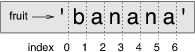
\includegraphics[scale=0.8]{../source/figs/banana.pdf}}
\caption{Slice indices.}
\label{fig.banana}
\end{figure}

If you omit the first index (before the colon), the slice starts at
the beginning of the string.  If you omit the second index, the slice
goes to the end of the string:

\begin{verbatim}
>>> fruit = 'banana'
>>> fruit[:3]
'ban'
>>> fruit[3:]
'ana'
\end{verbatim}
%
If the first index is greater than or equal to the second the result
is an {\bf empty string}, represented by two quotation marks:
\index{quotation mark}

\begin{verbatim}
>>> fruit = 'banana'
>>> fruit[3:3]
''
\end{verbatim}
%
An empty string contains no characters and has length 0, but other
than that, it is the same as any other string.

Continuing this example, what do you think
{\tt fruit[:]} means?  Try it and see.
\index{copy!slice}
\index{slice!copy}



\section{Strings are immutable}
\index{mutability}
\index{immutability}
\index{string!immutable}

It is tempting to use the {\tt []} operator on the left side of an
assignment, with the intention of changing a character in a string.
For example:
\index{TypeError}
\index{exception!TypeError}

\begin{verbatim}
>>> greeting = 'Hello, world!'
>>> greeting[0] = 'J'
TypeError: 'str' object does not support item assignment
\end{verbatim}
%
The ``object'' in this case is the string and the ``item'' is
the character you tried to assign.  For now, an object is
the same thing as a value, but we will refine that definition
later (Section~\ref{equivalence}).
\index{object}
\index{item}
\index{item assignment}
\index{assignment!item}
\index{immutability}

The reason for the error is that
strings are {\bf immutable}, which means you can't change an
existing string.  The best you can do is create a new string
that is a variation on the original:

\begin{verbatim}
>>> greeting = 'Hello, world!'
>>> new_greeting = 'J' + greeting[1:]
>>> new_greeting
'Jello, world!'
\end{verbatim}
%
This example concatenates a new first letter onto
a slice of {\tt greeting}.  It has no effect on
the original string.
\index{concatenation}


\section{Searching}
\label{find}

What does the following function do?
\index{find function}
\index{function!find}

\begin{verbatim}
def find(word, letter):
    index = 0
    while index < len(word):
        if word[index] == letter:
            return index
        index = index + 1
    return -1
\end{verbatim}
%
In a sense, {\tt find} is the inverse of the {\tt []} operator.
Instead of taking an index and extracting the corresponding character,
it takes a character and finds the index where that character
appears.  If the character is not found, the function returns {\tt
-1}.

This is the first example we have seen of a {\tt return} statement
inside a loop.  If {\tt word[index] == letter}, the function breaks
out of the loop and returns immediately.

If the character doesn't appear in the string, the program
exits the loop normally and  returns {\tt -1}.

This pattern of computation---traversing a sequence and returning
when we find what we are looking for---is called a {\bf search}.
\index{traversal}
\index{search pattern}
\index{pattern!search}

As an exercise, modify {\tt find} so that it has a
third parameter, the index in {\tt word} where it should start
looking.


\section{Looping and counting}
\label{counter}
\index{counter}
\index{counting and looping}
\index{looping and counting}
\index{looping!with strings}

The following program counts the number of times the letter {\tt a}
appears in a string:

\begin{verbatim}
word = 'banana'
count = 0
for letter in word:
    if letter == 'a':
        count = count + 1
print(count)
\end{verbatim}
%
This program demonstrates another pattern of computation called a {\bf
counter}.  The variable {\tt count} is initialized to 0 and then
incremented each time an {\tt a} is found.
When the loop exits, {\tt count}
contains the result---the total number of {\tt a}'s.

\index{encapsulation}
As an exercise, encapsulate this code in a function named {\tt
count}, and generalize it so that it accepts the string and the
letter as arguments.

Then rewrite the function so that instead of
traversing the string, it uses the three-parameter version of {\tt
find} from the previous section.


\section{String methods}
\label{optional}

Strings provide methods that perform a variety of useful operations.
A method is similar to a function---it takes arguments and
returns a value---but the syntax is different.  For example, the
method {\tt upper} takes a string and returns a new string with
all uppercase letters.
\index{method}
\index{string!method}

Instead of the function syntax {\tt upper(word)}, it uses
the method syntax {\tt word.upper()}.

\begin{verbatim}
>>> word = 'banana'
>>> new_word = word.upper()
>>> new_word
'BANANA'
\end{verbatim}
%
This form of dot notation specifies the name of the method, {\tt
upper}, and the name of the string to apply the method to, {\tt
word}.  The empty parentheses indicate that this method takes no
arguments.
\index{parentheses!empty}
\index{dot notation}

A method call is called an {\bf invocation}; in this case, we would
say that we are invoking {\tt upper} on {\tt word}.
\index{invocation}

As it turns out, there is a string method named {\tt find} that
is remarkably similar to the function we wrote:

\begin{verbatim}
>>> word = 'banana'
>>> index = word.find('a')
>>> index
1
\end{verbatim}
%
In this example, we invoke {\tt find} on {\tt word} and pass
the letter we are looking for as a parameter.

Actually, the {\tt find} method is more general than our function;
it can find substrings, not just characters:

\begin{verbatim}
>>> word.find('na')
2
\end{verbatim}
%
By default, {\tt find} starts at the beginning of the string, but
it can take a second argument, the index where it should start:
\index{optional argument}
\index{argument!optional}

\begin{verbatim}
>>> word.find('na', 3)
4
\end{verbatim}
%
This is an example of an {\bf optional argument};
{\tt find} can
also take a third argument, the index where it should stop:

\begin{verbatim}
>>> name = 'bob'
>>> name.find('b', 1, 2)
-1
\end{verbatim}
%
This search fails because {\tt b} does not
appear in the index range from {\tt 1} to {\tt 2}, not including {\tt
2}.  Searching up to, but not including, the second index makes
{\tt find} consistent with the slice operator.



\section{The {\tt in} operator}
\label{inboth}
\index{in operator}
\index{operator!in}
\index{boolean operator}
\index{operator!boolean}

The word {\tt in} is a boolean operator that takes two strings and
returns {\tt True} if the first appears as a substring in the second:

\begin{verbatim}
>>> 'a' in 'banana'
True
>>> 'seed' in 'banana'
False
\end{verbatim}
%
For example, the following function prints all the
letters from {\tt word1} that also appear in {\tt word2}:

\begin{verbatim}
def in_both(word1, word2):
    for letter in word1:
        if letter in word2:
            print(letter)
\end{verbatim}
%
With well-chosen variable names,
Python sometimes reads like English.  You could read
this loop, ``for (each) letter in (the first) word, if (the) letter
(appears) in (the second) word, print (the) letter.''

Here's what you get if you compare apples and oranges:

\begin{verbatim}
>>> in_both('apples', 'oranges')
a
e
s
\end{verbatim}
%

\section{String comparison}
\index{string!comparison}
\index{comparison!string}

The relational operators work on strings.  To see if two strings are equal:

\begin{verbatim}
if word == 'banana':
    print('All right, bananas.')
\end{verbatim}
%
Other relational operations are useful for putting words in alphabetical
order:

\begin{verbatim}
if word < 'banana':
    print('Your word, ' + word + ', comes before banana.')
elif word > 'banana':
    print('Your word, ' + word + ', comes after banana.')
else:
    print('All right, bananas.')
\end{verbatim}
%
Python does not handle uppercase and lowercase letters the same way
people do.  All the uppercase letters come before all the
lowercase letters, so:

\begin{verbatim}
Your word, Pineapple, comes before banana.
\end{verbatim}
%
A common way to address this problem is to convert strings to a
standard format, such as all lowercase, before performing the
comparison.  Keep that in mind in case you have to defend yourself
against a man armed with a Pineapple.


\section{Debugging}
\index{debugging}
\index{traversal}

When you use indices to traverse the values in a sequence,
it is tricky to get the beginning and end of the traversal
right.  Here is a function that is supposed to compare two
words and return {\tt True} if one of the words is the reverse
of the other, but it contains two errors:

\begin{verbatim}
def is_reverse(word1, word2):
    if len(word1) != len(word2):
        return False

    i = 0
    j = len(word2)

    while j > 0:
        if word1[i] != word2[j]:
            return False
        i = i+1
        j = j-1

    return True
\end{verbatim}
%
The first {\tt if} statement checks whether the words are the
same length.  If not, we can return {\tt False} immediately.
Otherwise, for the rest of the function, we can assume that the words
are the same length.  This is an example of the guardian pattern
in Section~\ref{guardian}.
\index{guardian pattern}
\index{pattern!guardian}
\index{index}

{\tt i} and {\tt j} are indices: {\tt i} traverses {\tt word1}
forward while {\tt j} traverses {\tt word2} backward.  If we find
two letters that don't match, we can return {\tt False} immediately.
If we get through the whole loop and all the letters match, we
return {\tt True}.

If we test this function with the words ``pots'' and ``stop'', we
expect the return value {\tt True}, but we get an IndexError:
\index{IndexError}
\index{exception!IndexError}

\begin{verbatim}
>>> is_reverse('pots', 'stop')
...
  File "reverse.py", line 15, in is_reverse
    if word1[i] != word2[j]:
IndexError: string index out of range
\end{verbatim}
%
For debugging this kind of error, my first move is to
print the values of the indices immediately before the line
where the error appears.

\begin{verbatim}
    while j > 0:
        print(i, j)        # print here

        if word1[i] != word2[j]:
            return False
        i = i+1
        j = j-1
\end{verbatim}
%
Now when I run the program again, I get more information:

\begin{verbatim}
>>> is_reverse('pots', 'stop')
0 4
...
IndexError: string index out of range
\end{verbatim}
%
The first time through the loop, the value of {\tt j} is 4,
which is out of range for the string \verb"'pots'".
The index of the last character is 3, so the
initial value for {\tt j} should be {\tt len(word2)-1}.

If I fix that error and run the program again, I get:

\begin{verbatim}
>>> is_reverse('pots', 'stop')
0 3
1 2
2 1
True
\end{verbatim}
%
This time we get the right answer, but it looks like the loop only ran
three times, which is suspicious.  To get a better idea of what is
happening, it is useful to draw a state diagram.  During the first
iteration, the frame for \verb"is_reverse" is shown in
Figure~\ref{fig.state4}.  \index{state diagram} \index{diagram!state}

\begin{figure}
\centerline
{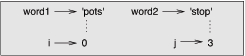
\includegraphics[scale=0.8]{../source/figs/state4.pdf}}
\caption{State diagram.}
\label{fig.state4}
\end{figure}

I took some license by arranging the variables in the frame
and adding dotted lines to show that the values of {\tt i} and
{\tt j} indicate characters in {\tt word1} and {\tt word2}.

Starting with this diagram, run the program on paper, changing the
values of {\tt i} and {\tt j} during each iteration.  Find and fix the
second error in this function.
\label{isreverse}


\section{Glossary}

\begin{description}

\item[object:] Something a variable can refer to.  For now,
you can use ``object'' and ``value'' interchangeably.
\index{object}

\item[sequence:] An ordered collection of
values where each value is identified by an integer index.
\index{sequence}

\item[item:] One of the values in a sequence.
\index{item}

\item[index:] An integer value used to select an item in
a sequence, such as a character in a string.  In Python
indices start from 0.
\index{index}

\item[slice:] A part of a string specified by a range of indices.
\index{slice}

\item[empty string:] A string with no characters and length 0, represented
by two quotation marks.
\index{empty string}

\item[immutable:] The property of a sequence whose items cannot
be changed.
\index{immutability}

\item[traverse:] To iterate through the items in a sequence,
performing a similar operation on each.
\index{traversal}

\item[search:] A pattern of traversal that stops
when it finds what it is looking for.
\index{search pattern}
\index{pattern!search}

\item[counter:] A variable used to count something, usually initialized
to zero and then incremented.
\index{counter}

\item[invocation:] A statement that calls a method.
\index{invocation}

\item[optional argument:] A function or method argument that is not
required.
\index{optional argument}
\index{argument!optional}

\end{description}


\section{Exercises}

\begin{exercise}
\index{string method}
\index{method!string}

Read the documentation of the string methods at
\url{http://docs.python.org/3/library/stdtypes.html#string-methods}.
You might want to experiment with some of them to make sure you
understand how they work.  {\tt strip} and {\tt replace} are
particularly useful.

The documentation uses a syntax that might be confusing.
For example, in \verb"find(sub[, start[, end]])", the brackets
indicate optional arguments.  So {\tt sub} is required, but
{\tt start} is optional, and if you include {\tt start},
then {\tt end} is optional.
\index{optional argument}
\index{argument!optional}

\end{exercise}


\begin{exercise}
\index{count method}
\index{method!count}

There is a string method called {\tt count} that is similar
to the function in Section~\ref{counter}.  Read the documentation
of this method
and write an invocation that counts the number of {\tt a}'s
in \verb"'banana'".
\end{exercise}


\begin{exercise}
\index{step size}
\index{slice operator}
\index{operator!slice}

A string slice can take a third index that specifies the ``step
size''; that is, the number of spaces between successive characters.
A step size of 2 means every other character; 3 means every third,
etc.

\begin{verbatim}
>>> fruit = 'banana'
>>> fruit[0:5:2]
'bnn'
\end{verbatim}

A step size of -1 goes through the word backwards, so
the slice \verb"[::-1]" generates a reversed string.
\index{palindrome}

Use this idiom to write a one-line version of \verb"is_palindrome"
from Exercise~\ref{palindrome}.
\end{exercise}


\begin{exercise}

The following functions are all {\em intended} to check whether a
string contains any lowercase letters, but at least some of them are
wrong.  For each function, describe what the function actually does
(assuming that the parameter is a string).

\begin{verbatim}
def any_lowercase1(s):
    for c in s:
        if c.islower():
            return True
        else:
            return False

def any_lowercase2(s):
    for c in s:
        if 'c'.islower():
            return 'True'
        else:
            return 'False'

def any_lowercase3(s):
    for c in s:
        flag = c.islower()
    return flag

def any_lowercase4(s):
    flag = False
    for c in s:
        flag = flag or c.islower()
    return flag

def any_lowercase5(s):
    for c in s:
        if not c.islower():
            return False
    return True
\end{verbatim}

\end{exercise}


\begin{exercise}
\index{letter rotation}
\index{rotation, letter}

\label{exrotate}
A Caesar cypher is a weak form of encryption that involves ``rotating'' each
letter by a fixed number of places.  To rotate a letter means
to shift it through the alphabet, wrapping around to the beginning if
necessary, so 'A' rotated by 3 is 'D' and 'Z' rotated by 1 is 'A'.

To rotate a word, rotate each letter by the same amount.
For example, ``cheer'' rotated by 7 is ``jolly'' and ``melon'' rotated
by -10 is ``cubed''.  In the movie {\em 2001: A Space Odyssey}, the
ship computer is called HAL, which is IBM rotated by -1.

%For example ``sleep''
%rotated by 9 is ``bunny'' and ``latex'' rotated by 7 is ``shale''.

Write a function called \verb"rotate_word"
that takes a string and an integer as parameters, and returns
a new string that contains the letters from the original string
rotated by the given amount.

You might want to use the built-in function {\tt ord}, which converts
a character to a numeric code, and {\tt chr}, which converts numeric
codes to characters.  Letters of the alphabet are encoded in alphabetical
order, so for example:

\begin{verbatim}
>>> ord('c') - ord('a')
2
\end{verbatim}

Because \verb"'c'" is the two-eth letter of the alphabet.  But
beware: the numeric codes for upper case letters are different.

Potentially offensive jokes on the Internet are sometimes encoded in
ROT13, which is a Caesar cypher with rotation 13.  If you are not
easily offended, find and decode some of them.  Solution:
\url{http://thinkpython2.com/code/rotate.py}.

\end{exercise}


\chapter{Case study: word play}
\label{wordplay}

This chapter presents the second case study, which involves
solving word puzzles by searching for words that have certain
properties.  For example, we'll find the longest palindromes
in English and search for words whose letters appear in
alphabetical order.  And I will present another program development
plan: reduction to a previously solved problem.


\section{Reading word lists}
\label{wordlist}

For the exercises in this chapter we need a list of English words.
There are lots of word lists available on the Web, but the one most
suitable for our purpose is one of the word lists collected and
contributed to the public domain by Grady Ward as part of the Moby
lexicon project (see \url{http://wikipedia.org/wiki/Moby_Project}).  It
is a list of 113,809 official crosswords; that is, words that are
considered valid in crossword puzzles and other word games.  In the
Moby collection, the filename is {\tt 113809of.fic}; you can download
a copy, with the simpler name {\tt words.txt}, from
\url{http://thinkpython2.com/code/words.txt}.
\index{Moby Project}
\index{crosswords}

This file is in plain text, so you can open it with a text
editor, but you can also read it from Python.  The built-in
function {\tt open} takes the name of the file as a parameter
and returns a {\bf file object} you can use to read the file.
\index{open function}
\index{function!open}
\index{plain text}
\index{text!plain}
\index{object!file}
\index{file object}

\begin{verbatim}
>>> fin = open('words.txt')
\end{verbatim}
%
{\tt fin} is a common name for a file object used for input.  The file
object provides several methods for reading, including {\tt readline},
which reads characters from the file until it gets to a newline and
returns the result as a string: \index{readline method}
\index{method!readline}

\begin{verbatim}
>>> fin.readline()
'aa\r\n'
\end{verbatim}
%
The first word in this particular list is ``aa'', which is a kind of
lava.  The sequence \verb"\r\n" represents two whitespace characters,
a carriage return and a newline, that separate this word from the
next.

The file object keeps track of where it is in the file, so
if you call {\tt readline} again, you get the next word:

\begin{verbatim}
>>> fin.readline()
'aah\r\n'
\end{verbatim}
%
The next word is ``aah'', which is a perfectly legitimate
word, so stop looking at me like that.
Or, if it's the whitespace that's bothering you,
we can get rid of it with the string method {\tt strip}:
\index{strip method}
\index{method!strip}

\begin{verbatim}
>>> line = fin.readline()
>>> word = line.strip()
>>> word
'aahed'
\end{verbatim}
%
You can also use a file object as part of a {\tt for} loop.
This program reads {\tt words.txt} and prints each word, one
per line:
\index{open function}
\index{function!open}

\begin{verbatim}
fin = open('words.txt')
for line in fin:
    word = line.strip()
    print(word)
\end{verbatim}
%

\section{Exercises}

There are solutions to these exercises in the next section.
You should at least attempt each one before you read the solutions.

\begin{exercise}
Write a program that reads {\tt words.txt} and prints only the
words with more than 20 characters (not counting whitespace).
\index{whitespace}

\end{exercise}

\begin{exercise}

In 1939 Ernest Vincent Wright published a 50,000 word novel called
{\em Gadsby} that does not contain the letter ``e''.  Since ``e'' is
the most common letter in English, that's not easy to do.

In fact, it is difficult to construct a solitary thought without using
that most common symbol.  It is slow going at first, but with caution
and hours of training you can gradually gain facility.

All right, I'll stop now.

Write a function called \verb"has_no_e" that returns {\tt True} if
the given word doesn't have the letter ``e'' in it.

Modify your program from the previous section to print only the words
that have no ``e'' and compute the percentage of the words in the list
that have no ``e''.
\index{lipogram}

\end{exercise}


\begin{exercise}

Write a function named {\tt avoids}
that takes a word and a string of forbidden letters, and
that returns {\tt True} if the word doesn't use any of the forbidden
letters.

Modify your program to prompt the user to enter a string
of forbidden letters and then print the number of words that
don't contain any of them.
Can you find a combination of 5 forbidden letters that
excludes the smallest number of words?

\end{exercise}



\begin{exercise}

Write a function named \verb"uses_only" that takes a word and a
string of letters, and that returns {\tt True} if the word contains
only letters in the list.  Can you make a sentence using only the
letters {\tt acefhlo}?  Other than ``Hoe alfalfa?''

\end{exercise}


\begin{exercise}

Write a function named \verb"uses_all" that takes a word and a
string of required letters, and that returns {\tt True} if the word
uses all the required letters at least once.  How many words are there
that use all the vowels {\tt aeiou}?  How about {\tt aeiouy}?

\end{exercise}


\begin{exercise}

Write a function called \verb"is_abecedarian" that returns
{\tt True} if the letters in a word appear in alphabetical order
(double letters are ok).
How many abecedarian words are there?

\index{abecedarian}

\end{exercise}



\section{Search}
\label{search}
\index{search pattern}
\index{pattern!search}

All of the exercises in the previous section have something
in common; they can be solved with the search pattern we saw
in Section~\ref{find}.  The simplest example is:

\begin{verbatim}
def has_no_e(word):
    for letter in word:
        if letter == 'e':
            return False
    return True
\end{verbatim}
%
The {\tt for} loop traverses the characters in {\tt word}.  If we find
the letter ``e'', we can immediately return {\tt False}; otherwise we
have to go to the next letter.  If we exit the loop normally, that
means we didn't find an ``e'', so we return {\tt True}.
\index{traversal}

\index{in operator}
\index{operator!in}
You could write this function more concisely using the {\tt in}
operator, but I started with this version because it
demonstrates the logic of the search pattern.

\index{generalization}
{\tt avoids} is a more general version of \verb"has_no_e" but it
has the same structure:

\begin{verbatim}
def avoids(word, forbidden):
    for letter in word:
        if letter in forbidden:
            return False
    return True
\end{verbatim}
%
We can return {\tt False} as soon as we find a forbidden letter;
if we get to the end of the loop, we return {\tt True}.

\verb"uses_only" is similar except that the sense of the condition
is reversed:

\begin{verbatim}
def uses_only(word, available):
    for letter in word:
        if letter not in available:
            return False
    return True
\end{verbatim}
%
Instead of a list of forbidden letters, we have a list of available
letters.  If we find a letter in {\tt word} that is not in
{\tt available}, we can return {\tt False}.

\verb"uses_all" is similar except that we reverse the role
of the word and the string of letters:

\begin{verbatim}
def uses_all(word, required):
    for letter in required:
        if letter not in word:
            return False
    return True
\end{verbatim}
%
Instead of traversing the letters in {\tt word}, the loop
traverses the required letters.  If any of the required letters
do not appear in the word, we can return {\tt False}.
\index{traversal}

If you were really thinking like a computer scientist, you would
have recognized that \verb"uses_all" was an instance of a
previously solved problem, and you would have written:

\begin{verbatim}
def uses_all(word, required):
    return uses_only(required, word)
\end{verbatim}
%
This is an example of a program development plan called {\bf
  reduction to a previously solved problem}, which means that you
recognize the problem you are working on as an instance of a solved
problem and apply an existing solution.  \index{reduction to a
  previously solved problem} \index{development plan!reduction}


\section{Looping with indices}
\index{looping!with indices}
\index{index!looping with}

I wrote the functions in the previous section with {\tt for}
loops because I only needed the characters in the strings; I didn't
have to do anything with the indices.

For \verb"is_abecedarian" we have to compare adjacent letters,
which is a little tricky with a {\tt for} loop:

\begin{verbatim}
def is_abecedarian(word):
    previous = word[0]
    for c in word:
        if c < previous:
            return False
        previous = c
    return True
\end{verbatim}

An alternative is to use recursion:

\begin{verbatim}
def is_abecedarian(word):
    if len(word) <= 1:
        return True
    if word[0] > word[1]:
        return False
    return is_abecedarian(word[1:])
\end{verbatim}

Another option is to use a {\tt while} loop:

\begin{verbatim}
def is_abecedarian(word):
    i = 0
    while i < len(word)-1:
        if word[i+1] < word[i]:
            return False
        i = i+1
    return True
\end{verbatim}
%
The loop starts at {\tt i=0} and ends when {\tt i=len(word)-1}.  Each
time through the loop, it compares the $i$th character (which you can
think of as the current character) to the $i+1$th character (which you
can think of as the next).

If the next character is less than (alphabetically before) the current
one, then we have discovered a break in the abecedarian trend, and
we return {\tt False}.

If we get to the end of the loop without finding a fault, then the
word passes the test.  To convince yourself that the loop ends
correctly, consider an example like \verb"'flossy'".  The
length of the word is 6, so
the last time the loop runs is when {\tt i} is 4, which is the
index of the second-to-last character.  On the last iteration,
it compares the second-to-last character to the last, which is
what we want.
\index{palindrome}

Here is a version of \verb"is_palindrome" (see
Exercise~\ref{palindrome}) that uses two indices; one starts at the
beginning and goes up; the other starts at the end and goes down.

\begin{verbatim}
def is_palindrome(word):
    i = 0
    j = len(word)-1

    while i<j:
        if word[i] != word[j]:
            return False
        i = i+1
        j = j-1

    return True
\end{verbatim}

Or we could reduce to a previously solved
problem and write:
\index{reduction to a previously solved problem}
\index{development plan!reduction}

\begin{verbatim}
def is_palindrome(word):
    return is_reverse(word, word)
\end{verbatim}
%
Using \verb"is_reverse" from Section~\ref{isreverse}.


\section{Debugging}
\index{debugging}
\index{testing!is hard}
\index{program testing}

Testing programs is hard.  The functions in this chapter are
relatively easy to test because you can check the results by hand.
Even so, it is somewhere between difficult and impossible to choose a
set of words that test for all possible errors.

Taking \verb"has_no_e" as an example, there are two obvious
cases to check: words that have an `e' should return {\tt False}, and
words that don't should return {\tt True}.  You should have no
trouble coming up with one of each.

Within each case, there are some less obvious subcases.  Among the
words that have an ``e'', you should test words with an ``e'' at the
beginning, the end, and somewhere in the middle.  You should test long
words, short words, and very short words, like the empty string.  The
empty string is an example of a {\bf special case}, which is one of
the non-obvious cases where errors often lurk.
\index{special case}

In addition to the test cases you generate, you can also test
your program with a word list like {\tt words.txt}.  By scanning
the output, you might be able to catch errors, but be careful:
you might catch one kind of error (words that should not be
included, but are) and not another (words that should be included,
but aren't).

In general, testing can help you find bugs, but it is not easy to
generate a good set of test cases, and even if you do, you can't
be sure your program is correct.
According to a legendary computer scientist:
\index{testing!and absence of bugs}

\begin{quote}
Program testing can be used to show the presence of bugs, but never to
show their absence!

--- Edsger W. Dijkstra
\end{quote}
\index{Dijkstra, Edsger}


\section{Glossary}

\begin{description}

\item[file object:] A value that represents an open file.
\index{file object}
\index{object!file}

\item[reduction to a previously solved problem:] A way of solving a
  problem by expressing it as an instance of a previously solved
  problem.  \index{reduction to a previously solved problem}
  \index{development plan!reduction}

\item[special case:] A test case that is atypical or non-obvious
(and less likely to be handled correctly).
\index{special case}

\end{description}


\section{Exercises}

\begin{exercise}
\index{Car Talk}
\index{Puzzler}
\index{double letters}

This question is based on a Puzzler that was broadcast on the radio
program {\em Car Talk}
(\url{http://www.cartalk.com/content/puzzlers}):

\begin{quote}
Give me a word with three consecutive double letters. I'll give you a
couple of words that almost qualify, but don't. For example, the word
committee, c-o-m-m-i-t-t-e-e. It would be great except for the `i' that
sneaks in there. Or Mississippi: M-i-s-s-i-s-s-i-p-p-i. If you could
take out those i's it would work. But there is a word that has three
consecutive pairs of letters and to the best of my knowledge this may
be the only word. Of course there are probably 500 more but I can only
think of one. What is the word?
\end{quote}

Write a program to find it.
Solution: \url{http://thinkpython2.com/code/cartalk1.py}.

\end{exercise}


\begin{exercise}
Here's another {\em Car Talk}
Puzzler (\url{http://www.cartalk.com/content/puzzlers}):
\index{Car Talk}
\index{Puzzler}
\index{odometer}
\index{palindrome}

\begin{quote}
``I was driving on the highway the other day and I happened to
notice my odometer. Like most odometers, it shows six digits,
in whole miles only. So, if my car had 300,000
miles, for example, I'd see 3-0-0-0-0-0.

``Now, what I saw that day was very interesting. I noticed that the
last 4 digits were palindromic; that is, they read the same forward as
backward. For example, 5-4-4-5 is a palindrome, so my odometer
could have read 3-1-5-4-4-5.

``One mile later, the last 5 numbers were palindromic. For example, it
could have read 3-6-5-4-5-6.  One mile after that, the middle 4 out of
6 numbers were palindromic.  And you ready for this? One mile later,
all 6 were palindromic!

``The question is, what was on the odometer when I first looked?''
\end{quote}

Write a Python program that tests all the six-digit numbers and prints
any numbers that satisfy these requirements.
Solution: \url{http://thinkpython2.com/code/cartalk2.py}.

\end{exercise}


\begin{exercise}
Here's another {\em Car Talk} Puzzler you can solve with a
search (\url{http://www.cartalk.com/content/puzzlers}):
\index{Car Talk}
\index{Puzzler}
\index{palindrome}

\begin{quote}
``Recently I had a visit with my mom and we realized that
the two digits that make up my age when reversed resulted in her
age. For example, if she's 73, I'm 37. We wondered how often this has
happened over the years but we got sidetracked with other topics and
we never came up with an answer.

``When I got home I figured out that the digits of our ages have been
reversible six times so far. I also figured out that if we're lucky it
would happen again in a few years, and if we're really lucky it would
happen one more time after that. In other words, it would have
happened 8 times over all. So the question is, how old am I now?''

\end{quote}

Write a Python program that searches for solutions to this Puzzler.
Hint: you might find the string method {\tt zfill} useful.

Solution: \url{http://thinkpython2.com/code/cartalk3.py}.

\end{exercise}



\chapter{Lists}

This chapter presents one of Python's most useful built-in types, lists.
You will also learn more about objects and what can happen when you have
more than one name for the same object.


\section{A list is a sequence}
\label{sequence}

Like a string, a {\bf list} is a sequence of values.  In a string, the
values are characters; in a list, they can be any type.  The values in
a list are called {\bf elements} or sometimes {\bf items}.
\index{list}
\index{type!list}
\index{element}
\index{sequence}
\index{item}

There are several ways to create a new list; the simplest is to
enclose the elements in square brackets (\verb"[" and \verb"]"):

\begin{verbatim}
[10, 20, 30, 40]
['crunchy frog', 'ram bladder', 'lark vomit']
\end{verbatim}
%
The first example is a list of four integers.  The second is a list of
three strings.  The elements of a list don't have to be the same type.
The following list contains a string, a float, an integer, and
(lo!) another list:

\begin{verbatim}
['spam', 2.0, 5, [10, 20]]
\end{verbatim}
%
A list within another list is {\bf nested}.
\index{nested list}
\index{list!nested}

A list that contains no elements is
called an empty list; you can create one with empty
brackets, \verb"[]".
\index{empty list}
\index{list!empty}

As you might expect, you can assign list values to variables:

\begin{verbatim}
>>> cheeses = ['Cheddar', 'Edam', 'Gouda']
>>> numbers = [42, 123]
>>> empty = []
>>> print(cheeses, numbers, empty)
['Cheddar', 'Edam', 'Gouda'] [42, 123] []
\end{verbatim}
%
\index{assignment}


\section{Lists are mutable}
\label{mutable}
\index{list!element}
\index{access}
\index{index}
\index{bracket operator}
\index{operator!bracket}

The syntax for accessing the elements of a list is the same as for
accessing the characters of a string---the bracket operator.  The
expression inside the brackets specifies the index.  Remember that the
indices start at 0:

\begin{verbatim}
>>> cheeses[0]
'Cheddar'
\end{verbatim}
%
Unlike strings, lists are mutable.  When the bracket operator appears
on the left side of an assignment, it identifies the element of the
list that will be assigned.
\index{mutability}

\begin{verbatim}
>>> numbers = [42, 123]
>>> numbers[1] = 5
>>> numbers
[42, 5]
\end{verbatim}
%
The one-eth element of {\tt numbers}, which
used to be 123, is now 5.
\index{index!starting at zero}
\index{zero, index starting at}

Figure~\ref{fig.liststate} shows
the state diagram for {\tt
cheeses}, {\tt numbers} and {\tt empty}:
\index{state diagram}
\index{diagram!state}

\begin{figure}
\centerline
{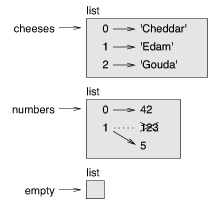
\includegraphics[scale=0.8]{../source/figs/liststate.pdf}}
\caption{State diagram.}
\label{fig.liststate}
\end{figure}

Lists are represented by boxes with the word ``list'' outside
and the elements of the list inside.  {\tt cheeses} refers to
a list with three elements indexed 0, 1 and 2.
{\tt numbers} contains two elements; the diagram shows that the
value of the second element has been reassigned from 123 to 5.
{\tt empty} refers to a list with no elements.
\index{item assignment}
\index{assignment!item}
\index{reassignment}

List indices work the same way as string indices:

\begin{itemize}

\item Any integer expression can be used as an index.

\item If you try to read or write an element that does not exist, you
get an {\tt IndexError}.
\index{exception!IndexError}
\index{IndexError}

\item If an index has a negative value, it counts backward from the
end of the list.

\end{itemize}
\index{list!index}

\index{list!membership}
\index{membership!list}
\index{in operator}
\index{operator!in}

The {\tt in} operator also works on lists.

\begin{verbatim}
>>> cheeses = ['Cheddar', 'Edam', 'Gouda']
>>> 'Edam' in cheeses
True
>>> 'Brie' in cheeses
False
\end{verbatim}


\section{Traversing a list}
\index{list!traversal}
\index{traversal!list}
\index{for loop}
\index{loop!for}
\index{statement!for}

The most common way to traverse the elements of a list is
with a {\tt for} loop.  The syntax is the same as for strings:

\begin{verbatim}
for cheese in cheeses:
    print(cheese)
\end{verbatim}
%
This works well if you only need to read the elements of the
list.  But if you want to write or update the elements, you
need the indices.  A common way to do that is to combine
the built-in functions {\tt range} and {\tt len}:
\index{looping!with indices}
\index{index!looping with}

\begin{verbatim}
for i in range(len(numbers)):
    numbers[i] = numbers[i] * 2
\end{verbatim}
%
This loop traverses the list and updates each element.  {\tt len}
returns the number of elements in the list.  {\tt range} returns
a list of indices from 0 to $n-1$, where $n$ is the length of
the list.  Each time through the loop {\tt i} gets the index
of the next element.  The assignment statement in the body uses
{\tt i} to read the old value of the element and to assign the
new value.
\index{item update}
\index{update!item}

A {\tt for} loop over an empty list never runs the body:

\begin{verbatim}
for x in []:
    print('This never happens.')
\end{verbatim}
%
Although a list can contain another list, the nested
list still counts as a single element.  The length of this list is
four:
\index{nested list}
\index{list!nested}

\begin{verbatim}
['spam', 1, ['Brie', 'Roquefort', 'Pol le Veq'], [1, 2, 3]]
\end{verbatim}



\section{List operations}
\index{list!operation}

The {\tt +} operator concatenates lists:
\index{concatenation!list}
\index{list!concatenation}

\begin{verbatim}
>>> a = [1, 2, 3]
>>> b = [4, 5, 6]
>>> c = a + b
>>> c
[1, 2, 3, 4, 5, 6]
\end{verbatim}
%
The {\tt *} operator repeats a list a given number of times:
\index{repetition!list}
\index{list!repetition}

\begin{verbatim}
>>> [0] * 4
[0, 0, 0, 0]
>>> [1, 2, 3] * 3
[1, 2, 3, 1, 2, 3, 1, 2, 3]
\end{verbatim}
%
The first example repeats {\tt [0]} four times.  The second example
repeats the list {\tt [1, 2, 3]} three times.


\section{List slices}
\index{slice operator}
\index{operator!slice}
\index{index!slice}
\index{list!slice}
\index{slice!list}

The slice operator also works on lists:

\begin{verbatim}
>>> t = ['a', 'b', 'c', 'd', 'e', 'f']
>>> t[1:3]
['b', 'c']
>>> t[:4]
['a', 'b', 'c', 'd']
>>> t[3:]
['d', 'e', 'f']
\end{verbatim}
%
If you omit the first index, the slice starts at the beginning.
If you omit the second, the slice goes to the end.  So if you
omit both, the slice is a copy of the whole list.
\index{list!copy}
\index{slice!copy}
\index{copy!slice}

\begin{verbatim}
>>> t[:]
['a', 'b', 'c', 'd', 'e', 'f']
\end{verbatim}
%
Since lists are mutable, it is often useful to make a copy
before performing operations that modify lists.
\index{mutability}

A slice operator on the left side of an assignment
can update multiple elements:
\index{slice!update}
\index{update!slice}

\begin{verbatim}
>>> t = ['a', 'b', 'c', 'd', 'e', 'f']
>>> t[1:3] = ['x', 'y']
>>> t
['a', 'x', 'y', 'd', 'e', 'f']
\end{verbatim}
%

% You can add elements to a list by squeezing them into an empty
% slice:

% % \begin{verbatim}
% >>> t = ['a', 'd', 'e', 'f']
% >>> t[1:1] = ['b', 'c']
% >>> print t
% ['a', 'b', 'c', 'd', 'e', 'f']
% \end{verbatim}
% \afterverb
%
% And you can remove elements from a list by assigning the empty list to
% them:

% % \begin{verbatim}
% >>> t = ['a', 'b', 'c', 'd', 'e', 'f']
% >>> t[1:3] = []
% >>> print t
% ['a', 'd', 'e', 'f']
% \end{verbatim}
% \afterverb
%
% But both of those operations can be expressed more clearly
% with list methods.


\section{List methods}
\index{list!method}
\index{method, list}

Python provides methods that operate on lists.  For example,
{\tt append} adds a new element to the end of a list:
\index{append method}
\index{method!append}

\begin{verbatim}
>>> t = ['a', 'b', 'c']
>>> t.append('d')
>>> t
['a', 'b', 'c', 'd']
\end{verbatim}
%
{\tt extend} takes a list as an argument and appends all of
the elements:
\index{extend method}
\index{method!extend}

\begin{verbatim}
>>> t1 = ['a', 'b', 'c']
>>> t2 = ['d', 'e']
>>> t1.extend(t2)
>>> t1
['a', 'b', 'c', 'd', 'e']
\end{verbatim}
%
This example leaves {\tt t2} unmodified.

{\tt sort} arranges the elements of the list from low to high:
\index{sort method}
\index{method!sort}

\begin{verbatim}
>>> t = ['d', 'c', 'e', 'b', 'a']
>>> t.sort()
>>> t
['a', 'b', 'c', 'd', 'e']
\end{verbatim}
%
Most list methods are void; they modify the list and return {\tt None}.
If you accidentally write {\tt t = t.sort()}, you will be disappointed
with the result.
\index{void method}
\index{method!void}
\index{None special value}
\index{special value!None}


\section{Map, filter and reduce}
\label{filter}

To add up all the numbers in a list, you can use a loop like this:

% see add.py

\begin{verbatim}
def add_all(t):
    total = 0
    for x in t:
        total += x
    return total
\end{verbatim}
%
{\tt total} is initialized to 0.  Each time through the loop,
{\tt x} gets one element from the list.  The {\tt +=} operator
provides a short way to update a variable.  This
{\bf augmented assignment statement},
\index{update operator}
\index{operator!update}
\index{assignment!augmented}
\index{augmented assignment}

\begin{verbatim}
    total += x
\end{verbatim}
%
is equivalent to

\begin{verbatim}
    total = total + x
\end{verbatim}
%
As the loop runs, {\tt total} accumulates the sum of the
elements; a variable used this way is sometimes called an
{\bf accumulator}.
\index{accumulator!sum}

Adding up the elements of a list is such a common operation
that Python provides it as a built-in function, {\tt sum}:

\begin{verbatim}
>>> t = [1, 2, 3]
>>> sum(t)
6
\end{verbatim}
%
An operation like this that combines a sequence of elements into
a single value is sometimes called {\bf reduce}.
\index{reduce pattern}
\index{pattern!reduce}
\index{traversal}

Sometimes you want to traverse one list while building
another.  For example, the following function takes a list of strings
and returns a new list that contains capitalized strings:

\begin{verbatim}
def capitalize_all(t):
    res = []
    for s in t:
        res.append(s.capitalize())
    return res
\end{verbatim}
%
{\tt res} is initialized with an empty list; each time through
the loop, we append the next element.  So {\tt res} is another
kind of accumulator.
\index{accumulator!list}

An operation like \verb"capitalize_all" is sometimes called a {\bf
map} because it ``maps'' a function (in this case the method {\tt
capitalize}) onto each of the elements in a sequence.
\index{map pattern}
\index{pattern!map}
\index{filter pattern}
\index{pattern!filter}

Another common operation is to select some of the elements from
a list and return a sublist.  For example, the following
function takes a list of strings and returns a list that contains
only the uppercase strings:

\begin{verbatim}
def only_upper(t):
    res = []
    for s in t:
        if s.isupper():
            res.append(s)
    return res
\end{verbatim}
%
{\tt isupper} is a string method that returns {\tt True} if
the string contains only upper case letters.

An operation like \verb"only_upper" is called a {\bf filter} because
it selects some of the elements and filters out the others.

Most common list operations can be expressed as a combination
of map, filter and reduce.


\section{Deleting elements}
\index{element deletion}
\index{deletion, element of list}

There are several ways to delete elements from a list.  If you
know the index of the element you want, you can use
{\tt pop}:
\index{pop method}
\index{method!pop}

\begin{verbatim}
>>> t = ['a', 'b', 'c']
>>> x = t.pop(1)
>>> t
['a', 'c']
>>> x
'b'
\end{verbatim}
%
{\tt pop} modifies the list and returns the element that was removed.
If you don't provide an index, it deletes and returns the
last element.

If you don't need the removed value, you can use the {\tt del}
operator:
\index{del operator}
\index{operator!del}

\begin{verbatim}
>>> t = ['a', 'b', 'c']
>>> del t[1]
>>> t
['a', 'c']
\end{verbatim}
%
If you know the element you want to remove (but not the index), you
can use {\tt remove}:
\index{remove method}
\index{method!remove}

\begin{verbatim}
>>> t = ['a', 'b', 'c']
>>> t.remove('b')
>>> t
['a', 'c']
\end{verbatim}
%
The return value from {\tt remove} is {\tt None}.
\index{None special value}
\index{special value!None}

To remove more than one element, you can use {\tt del} with
a slice index:

\begin{verbatim}
>>> t = ['a', 'b', 'c', 'd', 'e', 'f']
>>> del t[1:5]
>>> t
['a', 'f']
\end{verbatim}
%
As usual, the slice selects all the elements up to but not
including the second index.



\section{Lists and strings}
\index{list}
\index{string}
\index{sequence}

A string is a sequence of characters and a list is a sequence
of values, but a list of characters is not the same as a
string.  To convert from a string to a list of characters,
you can use {\tt list}:
\index{list!function}
\index{function!list}

\begin{verbatim}
>>> s = 'spam'
>>> t = list(s)
>>> t
['s', 'p', 'a', 'm']
\end{verbatim}
%
Because {\tt list} is the name of a built-in function, you should
avoid using it as a variable name.  I also avoid {\tt l} because
it looks too much like {\tt 1}.  So that's why I use {\tt t}.

The {\tt list} function breaks a string into individual letters.  If
you want to break a string into words, you can use the {\tt split}
method:
\index{split method}
\index{method!split}

\begin{verbatim}
>>> s = 'pining for the fjords'
>>> t = s.split()
>>> t
['pining', 'for', 'the', 'fjords']
\end{verbatim}
%
An optional argument called a {\bf delimiter} specifies which
characters to use as word boundaries.
The following example
uses a hyphen as a delimiter:
\index{optional argument}
\index{argument!optional}
\index{delimiter}

\begin{verbatim}
>>> s = 'spam-spam-spam'
>>> delimiter = '-'
>>> t = s.split(delimiter)
>>> t
['spam', 'spam', 'spam']
\end{verbatim}
%
{\tt join} is the inverse of {\tt split}.  It
takes a list of strings and
concatenates the elements.  {\tt join} is a string method,
so you have to invoke it on the delimiter and pass the
list as a parameter:
\index{join method}
\index{method!join}
\index{concatenation}

\begin{verbatim}
>>> t = ['pining', 'for', 'the', 'fjords']
>>> delimiter = ' '
>>> s = delimiter.join(t)
>>> s
'pining for the fjords'
\end{verbatim}
%
In this case the delimiter is a space character, so
{\tt join} puts a space between words.  To concatenate
strings without spaces, you can use the empty string,
\verb"''", as a delimiter.
\index{empty string}
\index{string!empty}


\section{Objects and values}
\label{equivalence}
\index{object}
\index{value}

If we run these assignment statements:

\begin{verbatim}
a = 'banana'
b = 'banana'
\end{verbatim}
%
We know that {\tt a} and {\tt b} both refer to a
string, but we don't
know whether they refer to the {\em same} string.
There are two possible states, shown in Figure~\ref{fig.list1}.
\index{aliasing}

\begin{figure}
\centerline
{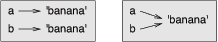
\includegraphics[scale=0.8]{../source/figs/list1.pdf}}
\caption{State diagram.}
\label{fig.list1}
\end{figure}

In one case, {\tt a} and {\tt b} refer to two different objects that
have the same value.  In the second case, they refer to the same
object.
\index{is operator}
\index{operator!is}

To check whether two variables refer to the same object, you can
use the {\tt is} operator.

\begin{verbatim}
>>> a = 'banana'
>>> b = 'banana'
>>> a is b
True
\end{verbatim}
%
In this example, Python only created one string object, and both {\tt
  a} and {\tt b} refer to it.  But when you create two lists, you get
two objects:

\begin{verbatim}
>>> a = [1, 2, 3]
>>> b = [1, 2, 3]
>>> a is b
False
\end{verbatim}
%
So the state diagram looks like Figure~\ref{fig.list2}.
\index{state diagram}
\index{diagram!state}

\begin{figure}
\centerline
{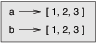
\includegraphics[scale=0.8]{../source/figs/list2.pdf}}
\caption{State diagram.}
\label{fig.list2}
\end{figure}

In this case we would say that the two lists are {\bf equivalent},
because they have the same elements, but not {\bf identical}, because
they are not the same object.  If two objects are identical, they are
also equivalent, but if they are equivalent, they are not necessarily
identical.
\index{equivalence}
\index{identity}

Until now, we have been using ``object'' and ``value''
interchangeably, but it is more precise to say that an object has a
value.  If you evaluate {\tt [1, 2, 3]}, you get a list
object whose value is a sequence of integers.  If another
list has the same elements, we say it has the same value, but
it is not the same object.
\index{object}
\index{value}


\section{Aliasing}
\index{aliasing}
\index{reference!aliasing}

If {\tt a} refers to an object and you assign {\tt b = a},
then both variables refer to the same object:

\begin{verbatim}
>>> a = [1, 2, 3]
>>> b = a
>>> b is a
True
\end{verbatim}
%
The state diagram looks like Figure~\ref{fig.list3}.
\index{state diagram}
\index{diagram!state}

\begin{figure}
\centerline
{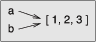
\includegraphics[scale=0.8]{../source/figs/list3.pdf}}
\caption{State diagram.}
\label{fig.list3}
\end{figure}

The association of a variable with an object is called a {\bf
reference}.  In this example, there are two references to the same
object.
\index{reference}

An object with more than one reference has more
than one name, so we say that the object is {\bf aliased}.
\index{mutability}

If the aliased object is mutable, changes made with one alias affect
the other:

\begin{verbatim}
>>> b[0] = 42
>>> a
[42, 2, 3]
\end{verbatim}
%
Although this behavior can be useful, it is error-prone.  In general,
it is safer to avoid aliasing when you are working with mutable
objects.
\index{immutability}

For immutable objects like strings, aliasing is not as much of a
problem.  In this example:

\begin{verbatim}
a = 'banana'
b = 'banana'
\end{verbatim}
%
It almost never makes a difference whether {\tt a} and {\tt b} refer
to the same string or not.


\section{List arguments}
\label{list.arguments}
\index{list!as argument}
\index{argument}
\index{argument!list}
\index{reference}
\index{parameter}

When you pass a list to a function, the function gets a reference to
the list.  If the function modifies the list, the caller sees
the change.  For example, \verb"delete_head" removes the first element
from a list:

\begin{verbatim}
def delete_head(t):
    del t[0]
\end{verbatim}
%
Here's how it is used:

\begin{verbatim}
>>> letters = ['a', 'b', 'c']
>>> delete_head(letters)
>>> letters
['b', 'c']
\end{verbatim}
%
The parameter {\tt t} and the variable {\tt letters} are
aliases for the same object.  The stack diagram looks like
Figure~\ref{fig.stack5}.
\index{stack diagram}
\index{diagram!stack}

\begin{figure}
\centerline
{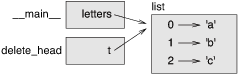
\includegraphics[scale=0.8]{../source/figs/stack5.pdf}}
\caption{Stack diagram.}
\label{fig.stack5}
\end{figure}

Since the list is shared by two frames, I drew
it between them.

It is important to distinguish between operations that
modify lists and operations that create new lists.  For
example, the {\tt append} method modifies a list, but the
{\tt +} operator creates a new list:
\index{append method}
\index{method!append}
\index{list!concatenation}
\index{concatenation!list}
%
\begin{verbatim}
>>> t1 = [1, 2]
>>> t2 = t1.append(3)
>>> t1
[1, 2, 3]
>>> t2
None
\end{verbatim}
%
{\tt append} modifies the list and returns {\tt None}.
%
\begin{verbatim}
>>> t3 = t1 + [4]
>>> t1
[1, 2, 3]
>>> t3
[1, 2, 3, 4]
>>> t1
\end{verbatim}
%
The {\tt +} operator creates a new list and leaves the
original list unchanged.

This difference is important when you write functions that
are supposed to modify lists.  For example, this function
{\em does not} delete the head of a list:
%
\begin{verbatim}
def bad_delete_head(t):
    t = t[1:]              # WRONG!
\end{verbatim}
%
The slice operator creates a new list and the assignment
makes {\tt t} refer to it, but that doesn't affect the caller.
\index{slice operator}
\index{operator!slice}
%
\begin{verbatim}
>>> t4 = [1, 2, 3]
>>> bad_delete_head(t4)
>>> t4
[1, 2, 3]
\end{verbatim}
%
At the beginning of \verb"bad_delete_head", {\tt t} and {\tt t4}
refer to the same list.  At the end, {\tt t} refers to a new list,
but {\tt t4} still refers to the original, unmodified list.

An alternative is to write a function that creates and
returns a new list.  For
example, {\tt tail} returns all but the first
element of a list:

\begin{verbatim}
def tail(t):
    return t[1:]
\end{verbatim}
%
This function leaves the original list unmodified.
Here's how it is used:

\begin{verbatim}
>>> letters = ['a', 'b', 'c']
>>> rest = tail(letters)
>>> rest
['b', 'c']
\end{verbatim}



\section{Debugging}
\index{debugging}

Careless use of lists (and other mutable objects)
can lead to long hours of debugging.  Here are some common
pitfalls and ways to avoid them:

\begin{enumerate}

\item Most list methods modify the argument and
  return {\tt None}.  This is the opposite of the string methods,
  which return a new string and leave the original alone.

If you are used to writing string code like this:

\begin{verbatim}
word = word.strip()
\end{verbatim}

It is tempting to write list code like this:

\begin{verbatim}
t = t.sort()           # WRONG!
\end{verbatim}
\index{sort method}
\index{method!sort}

Because {\tt sort} returns {\tt None}, the
next operation you perform with {\tt t} is likely to fail.

Before using list methods and operators, you should read the
documentation carefully and then test them in interactive mode.

\item Pick an idiom and stick with it.

Part of the problem with lists is that there are too many
ways to do things.  For example, to remove an element from
a list, you can use {\tt pop}, {\tt remove}, {\tt del},
or even a slice assignment.

To add an element, you can use the {\tt append} method or
the {\tt +} operator.  Assuming that {\tt t} is a list and
{\tt x} is a list element, these are correct:

\begin{verbatim}
t.append(x)
t = t + [x]
t += [x]
\end{verbatim}

And these are wrong:

\begin{verbatim}
t.append([x])          # WRONG!
t = t.append(x)        # WRONG!
t + [x]                # WRONG!
t = t + x              # WRONG!
\end{verbatim}

Try out each of these examples in interactive mode to make sure
you understand what they do.  Notice that only the last
one causes a runtime error; the other three are legal, but they
do the wrong thing.


\item Make copies to avoid aliasing.
\index{aliasing!copying to avoid}
\index{copy!to avoid aliasing}

If you want to use a method like {\tt sort} that modifies
the argument, but you need to keep the original list as
well, you can make a copy.

\begin{verbatim}
>>> t = [3, 1, 2]
>>> t2 = t[:]
>>> t2.sort()
>>> t
[3, 1, 2]
>>> t2
[1, 2, 3]
\end{verbatim}

In this example you could also use the built-in function {\tt sorted},
which returns a new, sorted list and leaves the original alone.

\begin{verbatim}
>>> t2 = sorted(t)
>>> t
[3, 1, 2]
>>> t2
[1, 2, 3]
\end{verbatim}

\end{enumerate}



\section{Glossary}

\begin{description}

\item[list:] A sequence of values.
\index{list}

\item[element:] One of the values in a list (or other sequence),
also called items.
\index{element}

\item[nested list:] A list that is an element of another list.
\index{nested list}

\item[accumulator:] A variable used in a loop to add up or
accumulate a result.
\index{accumulator}

\item[augmented assignment:] A statement that updates the value
of a variable using an operator like \verb"+=".
\index{assignment!augmented}
\index{augmented assignment}
\index{traversal}

\item[reduce:] A processing pattern that traverses a sequence
and accumulates the elements into a single result.
\index{reduce pattern}
\index{pattern!reduce}

\item[map:] A processing pattern that traverses a sequence and
performs an operation on each element.
\index{map pattern}
\index{pattern!map}

\item[filter:] A processing pattern that traverses a list and
selects the elements that satisfy some criterion.
\index{filter pattern}
\index{pattern!filter}

\item[object:] Something a variable can refer to.  An object
has a type and a value.
\index{object}

\item[equivalent:] Having the same value.
\index{equivalent}

\item[identical:] Being the same object (which implies equivalence).
\index{identical}

\item[reference:] The association between a variable and its value.
\index{reference}

\item[aliasing:] A circumstance where two or more variables refer to the same
object.
\index{aliasing}

\item[delimiter:] A character or string used to indicate where a
string should be split.
\index{delimiter}

\end{description}


\section{Exercises}

You can download solutions to these exercises from
\url{http://thinkpython2.com/code/list_exercises.py}.

\begin{exercise}

Write a function called \verb"nested_sum" that takes a list of lists
of integers and adds up the elements from all of the nested lists.
For example:

\begin{verbatim}
>>> t = [[1, 2], [3], [4, 5, 6]]
>>> nested_sum(t)
21
\end{verbatim}

\end{exercise}

\begin{exercise}
\label{cumulative}
\index{cumulative sum}

Write a function called {\tt cumsum} that takes a list of numbers and
returns the cumulative sum; that is, a new list where the $i$th
element is the sum of the first $i+1$ elements from the original list.
For example:

\begin{verbatim}
>>> t = [1, 2, 3]
>>> cumsum(t)
[1, 3, 6]
\end{verbatim}

\end{exercise}

\begin{exercise}

Write a function called \verb"middle" that takes a list and
returns a new list that contains all but the first and last
elements.  For example:

\begin{verbatim}
>>> t = [1, 2, 3, 4]
>>> middle(t)
[2, 3]
\end{verbatim}

\end{exercise}

\begin{exercise}

Write a function called \verb"chop" that takes a list, modifies it
by removing the first and last elements, and returns {\tt None}.
For example:

\begin{verbatim}
>>> t = [1, 2, 3, 4]
>>> chop(t)
>>> t
[2, 3]
\end{verbatim}

\end{exercise}


\begin{exercise}
Write a function called \verb"is_sorted" that takes a list as a
parameter and returns {\tt True} if the list is sorted in ascending
order and {\tt False} otherwise.  For example:

\begin{verbatim}
>>> is_sorted([1, 2, 2])
True
>>> is_sorted(['b', 'a'])
False
\end{verbatim}

\end{exercise}


\begin{exercise}
\label{anagram}
\index{anagram}

Two words are anagrams if you can rearrange the letters from one
to spell the other.  Write a function called \verb"is_anagram"
that takes two strings and returns {\tt True} if they are anagrams.
\end{exercise}



\begin{exercise}
\label{duplicate}
\index{duplicate}
\index{uniqueness}

Write a function called \verb"has_duplicates" that takes
a list and returns {\tt True} if there is any element that
appears more than once.  It should not modify the original
list.

\end{exercise}


\begin{exercise}

This exercise pertains to the so-called Birthday Paradox, which you
can read about at \url{http://en.wikipedia.org/wiki/Birthday_paradox}.
\index{birthday paradox}

If there are 23 students in your class, what are the chances
that two of you have the same birthday?  You can estimate this
probability by generating random samples of 23 birthdays
and checking for matches.  Hint: you can generate random birthdays
with the {\tt randint} function in the {\tt random} module.
\index{random module}
\index{module!random}
\index{randint function}
\index{function!randint}

You can download my
solution from \url{http://thinkpython2.com/code/birthday.py}.

\end{exercise}



\begin{exercise}
\index{append method}
\index{method append}
\index{list!concatenation}
\index{concatenation!list}

Write a function that reads the file {\tt words.txt} and builds
a list with one element per word.  Write two versions of
this function, one using the {\tt append} method and the
other using the idiom {\tt t = t + [x]}.  Which one takes
longer to run?  Why?

Solution: \url{http://thinkpython2.com/code/wordlist.py}.
\index{time module}
\index{module!time}

\end{exercise}


\begin{exercise}
\label{wordlist1}
\label{bisection}
\index{membership!bisection search}
\index{bisection search}
\index{search, bisection}
\index{membership!binary search}
\index{binary search}
\index{search, binary}

To check whether a word is in the word list, you could use
the {\tt in} operator, but it would be slow because it searches
through the words in order.

Because the words are in alphabetical order, we can speed things up
with a bisection search (also known as binary search), which is
similar to what you do when you look a word up in the dictionary.  You
start in the middle and check to see whether the word you are looking
for comes before the word in the middle of the list.  If so, you
search the first half of the list the same way.  Otherwise you search
the second half.

Either way, you cut the remaining search space in half.  If the
word list has 113,809 words, it will take about 17 steps to
find the word or conclude that it's not there.

Write a function called \verb"in_bisect" that takes a sorted list
and a target value and returns the index of the value
in the list if it's there, or {\tt None} if it's not.
\index{bisect module}
\index{module!bisect}

Or you could read the documentation of the {\tt bisect} module
and use that!  Solution: \url{http://thinkpython2.com/code/inlist.py}.

\end{exercise}

\begin{exercise}
\index{reverse word pair}

Two words are a ``reverse pair'' if each is the reverse of the
other.  Write a program that finds all the reverse pairs in the
word list.  Solution: \url{http://thinkpython2.com/code/reverse_pair.py}.

\end{exercise}

\begin{exercise}
\index{interlocking words}

Two words ``interlock'' if taking alternating letters from each forms
a new word.  For example, ``shoe'' and ``cold''
interlock to form ``schooled''.
Solution: \url{http://thinkpython2.com/code/interlock.py}.
Credit: This exercise is inspired by an example at \url{http://puzzlers.org}.

\begin{enumerate}

\item Write a program that finds all pairs of words that interlock.
  Hint: don't enumerate all pairs!

\item Can you find any words that are three-way interlocked; that is,
  every third letter forms a word, starting from the first, second or
  third?

\end{enumerate}
\end{exercise}


\chapter{Dictionaries}

This chapter presents another built-in type called a dictionary.
Dictionaries are one of Python's best features; they are the
building blocks of many efficient and elegant algorithms.


\section{A dictionary is a mapping}

\index{dictionary}
\index{dictionary}
\index{type!dict}
\index{key}
\index{key-value pair}
\index{index}
A {\bf dictionary} is like a list, but more general.  In a list,
the indices have to be integers; in a dictionary they can
be (almost) any type.

A dictionary contains a collection of indices, which are called {\bf
  keys}, and a collection of values.  Each key is associated with a
single value.  The association of a key and a value is called a {\bf
  key-value pair} or sometimes an {\bf item}.  \index{item}

In mathematical language, a dictionary represents a {\bf mapping}
from keys to values, so you can also say that each key
``maps to'' a value.
As an example, we'll build a dictionary that maps from English
to Spanish words, so the keys and the values are all strings.

The function {\tt dict} creates a new dictionary with no items.
Because {\tt dict} is the name of a built-in function, you
should avoid using it as a variable name.
\index{dict function}
\index{function!dict}

\begin{verbatim}
>>> eng2sp = dict()
>>> eng2sp
{}
\end{verbatim}

The squiggly-brackets, \verb"{}", represent an empty dictionary.
To add items to the dictionary, you can use square brackets:
\index{squiggly bracket}
\index{bracket!squiggly}

\begin{verbatim}
>>> eng2sp['one'] = 'uno'
\end{verbatim}
%
This line creates an item that maps from the key
\verb"'one'" to the value \verb"'uno'".  If we print the
dictionary again, we see a key-value pair with a colon
between the key and value:

\begin{verbatim}
>>> eng2sp
{'one': 'uno'}
\end{verbatim}
%
This output format is also an input format.  For example,
you can create a new dictionary with three items:

\begin{verbatim}
>>> eng2sp = {'one': 'uno', 'two': 'dos', 'three': 'tres'}
\end{verbatim}
%
But if you print {\tt eng2sp}, you might be surprised:

\begin{verbatim}
>>> eng2sp
{'one': 'uno', 'three': 'tres', 'two': 'dos'}
\end{verbatim}
%
The order of the key-value pairs might not be the same.  If
you type the same example on your computer, you might get a
different result.  In general, the order of items in
a dictionary is unpredictable.

But that's not a problem because
the elements of a dictionary are never indexed with integer indices.
Instead, you use the keys to look up the corresponding values:

\begin{verbatim}
>>> eng2sp['two']
'dos'
\end{verbatim}
%
The key \verb"'two'" always maps to the value \verb"'dos'" so the order
of the items doesn't matter.

If the key isn't in the dictionary, you get an exception:
\index{exception!KeyError}
\index{KeyError}

\begin{verbatim}
>>> eng2sp['four']
KeyError: 'four'
\end{verbatim}
%
The {\tt len} function works on dictionaries; it returns the
number of key-value pairs:
\index{len function}
\index{function!len}

\begin{verbatim}
>>> len(eng2sp)
3
\end{verbatim}
%
The {\tt in} operator works on dictionaries, too; it tells you whether
something appears as a {\em key} in the dictionary (appearing
as a value is not good enough).
\index{membership!dictionary}
\index{in operator}
\index{operator!in}

\begin{verbatim}
>>> 'one' in eng2sp
True
>>> 'uno' in eng2sp
False
\end{verbatim}
%
To see whether something appears as a value in a dictionary, you
can use the method {\tt values}, which returns a collection of
values, and then use the {\tt in} operator:
\index{values method}
\index{method!values}

\begin{verbatim}
>>> vals = eng2sp.values()
>>> 'uno' in vals
True
\end{verbatim}
%
The {\tt in} operator uses different algorithms for lists and
dictionaries.  For lists, it searches the elements of the list in
order, as in Section~\ref{find}.  As the list gets longer, the search
time gets longer in direct proportion.

For dictionaries, Python uses an
algorithm called a {\bf hashtable} that has a remarkable property: the
{\tt in} operator takes about the same amount of time no matter how
many items are in the dictionary.  I explain how that's possible
in Section~\ref{hashtable}, but the explanation might not make
sense until you've read a few more chapters.


\section{Dictionary as a collection of counters}
\label{histogram}
\index{counter}

Suppose you are given a string and you want to count how many
times each letter appears.  There are several ways you could do it:

\begin{enumerate}

\item You could create 26 variables, one for each letter of the
alphabet.  Then you could traverse the string and, for each
character, increment the corresponding counter, probably using
a chained conditional.

\item You could create a list with 26 elements.  Then you could
convert each character to a number (using the built-in function
{\tt ord}), use the number as an index into the list, and increment
the appropriate counter.

\item You could create a dictionary with characters as keys
and counters as the corresponding values.  The first time you
see a character, you would add an item to the dictionary.  After
that you would increment the value of an existing item.

\end{enumerate}

Each of these options performs the same computation, but each
of them implements that computation in a different way.
\index{implementation}

An {\bf implementation} is a way of performing a computation;
some implementations are better than others.  For example,
an advantage of the dictionary implementation is that we don't
have to know ahead of time which letters appear in the string
and we only have to make room for the letters that do appear.

Here is what the code might look like:

\begin{verbatim}
def histogram(s):
    d = dict()
    for c in s:
        if c not in d:
            d[c] = 1
        else:
            d[c] += 1
    return d
\end{verbatim}
%
The name of the function is {\tt histogram}, which is a statistical
term for a collection of counters (or frequencies).
\index{histogram}
\index{frequency}
\index{traversal}

The first line of the
function creates an empty dictionary.  The {\tt for} loop traverses
the string.  Each time through the loop, if the character {\tt c} is
not in the dictionary, we create a new item with key {\tt c} and the
initial value 1 (since we have seen this letter once).  If {\tt c} is
already in the dictionary we increment {\tt d[c]}.
\index{histogram}

Here's how it works:

\begin{verbatim}
>>> h = histogram('brontosaurus')
>>> h
{'a': 1, 'b': 1, 'o': 2, 'n': 1, 's': 2, 'r': 2, 'u': 2, 't': 1}
\end{verbatim}
%
The histogram indicates that the letters \verb"'a'" and \verb"'b'"
appear once; \verb"'o'" appears twice, and so on.


\index{get method}
\index{method!get}
Dictionaries have a method called {\tt get} that takes a key
and a default value.  If the key appears in the dictionary,
{\tt get} returns the corresponding value; otherwise it returns
the default value.  For example:

\begin{verbatim}
>>> h = histogram('a')
>>> h
{'a': 1}
>>> h.get('a', 0)
1
>>> h.get('b', 0)
0
\end{verbatim}
%
As an exercise, use {\tt get} to write {\tt histogram} more concisely.  You
should be able to eliminate the {\tt if} statement.


\section{Looping and dictionaries}
\index{dictionary!looping with}
\index{looping!with dictionaries}
\index{traversal}

If you use a dictionary in a {\tt for} statement, it traverses
the keys of the dictionary.  For example, \verb"print_hist"
prints each key and the corresponding value:

\begin{verbatim}
def print_hist(h):
    for c in h:
        print(c, h[c])
\end{verbatim}
%
Here's what the output looks like:

\begin{verbatim}
>>> h = histogram('parrot')
>>> print_hist(h)
a 1
p 1
r 2
t 1
o 1
\end{verbatim}
%
Again, the keys are in no particular order.  To traverse the keys
in sorted order, you can use the built-in function {\tt sorted}:
\index{keys method}
\index{method!keys}

\begin{verbatim}
>>> for key in sorted(h):
...     print(key, h[key])
a 1
o 1
p 1
r 2
t 1
\end{verbatim}

%TODO: get this on Atlas


\section{Reverse lookup}
\label{raise}
\index{dictionary!lookup}
\index{dictionary!reverse lookup}
\index{lookup, dictionary}
\index{reverse lookup, dictionary}

Given a dictionary {\tt d} and a key {\tt k}, it is easy to
find the corresponding value {\tt v = d[k]}.  This operation
is called a {\bf lookup}.

But what if you have {\tt v} and you want to find {\tt k}?
You have two problems: first, there might be more than one
key that maps to the value {\tt v}.  Depending on the application,
you might be able to pick one, or you might have to make
a list that contains all of them.  Second, there is no
simple syntax to do a {\bf reverse lookup}; you have to search.

Here is a function that takes a value and returns the first
key that maps to that value:

\begin{verbatim}
def reverse_lookup(d, v):
    for k in d:
        if d[k] == v:
            return k
    raise LookupError()
\end{verbatim}
%
This function is yet another example of the search pattern, but it
uses a feature we haven't seen before, {\tt raise}.  The
{\bf raise statement} causes an exception; in this case it causes a
{\tt LookupError}, which is a built-in exception used to indicate
that a lookup operation failed.
\index{search}
\index{pattern!search} \index{raise statement} \index{statement!raise}
\index{exception!LookupError} \index{LookupError}

If we get to the end of the loop, that means {\tt v}
doesn't appear in the dictionary as a value, so we raise an
exception.

Here is an example of a successful reverse lookup:

\begin{verbatim}
>>> h = histogram('parrot')
>>> key = reverse_lookup(h, 2)
>>> key
'r'
\end{verbatim}
%
And an unsuccessful one:

\begin{verbatim}
>>> key = reverse_lookup(h, 3)
Traceback (most recent call last):
  File "<stdin>", line 1, in <module>
  File "<stdin>", line 5, in reverse_lookup
LookupError
\end{verbatim}
%
The effect when you raise an exception is the same as when
Python raises one: it prints a traceback and an error message.
\index{traceback}
\index{optional argument}
\index{argument!optional}

The {\tt raise} statement can take a detailed error message as an
optional argument.  For example:

\begin{verbatim}
>>> raise LookupError('value does not appear in the dictionary')
Traceback (most recent call last):
  File "<stdin>", line 1, in ?
LookupError: value does not appear in the dictionary
\end{verbatim}
%
A reverse lookup is much slower than a forward lookup; if you
have to do it often, or if the dictionary gets big, the performance
of your program will suffer.


\section{Dictionaries and lists}
\label{invert}

Lists can appear as values in a dictionary.  For example, if you
are given a dictionary that maps from letters to frequencies, you
might want to invert it; that is, create a dictionary that maps
from frequencies to letters.  Since there might be several letters
with the same frequency, each value in the inverted dictionary
should be a list of letters.
\index{invert dictionary}
\index{dictionary!invert}

Here is a function that inverts a dictionary:

\begin{verbatim}
def invert_dict(d):
    inverse = dict()
    for key in d:
        val = d[key]
        if val not in inverse:
            inverse[val] = [key]
        else:
            inverse[val].append(key)
    return inverse
\end{verbatim}
%
Each time through the loop, {\tt key} gets a key from {\tt d} and
{\tt val} gets the corresponding value.  If {\tt val} is not in {\tt
  inverse}, that means we haven't seen it before, so we create a new
item and initialize it with a {\bf singleton} (a list that contains a
single element).  Otherwise we have seen this value before, so we
append the corresponding key to the list.  \index{singleton}

Here is an example:

\begin{verbatim}
>>> hist = histogram('parrot')
>>> hist
{'a': 1, 'p': 1, 'r': 2, 't': 1, 'o': 1}
>>> inverse = invert_dict(hist)
>>> inverse
{1: ['a', 'p', 't', 'o'], 2: ['r']}
\end{verbatim}

\begin{figure}
\centerline
{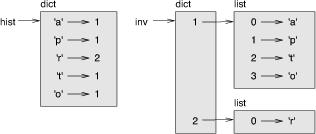
\includegraphics[scale=0.8]{../source/figs/dict1.pdf}}
\caption{State diagram.}
\label{fig.dict1}
\end{figure}

Figure~\ref{fig.dict1} is a state diagram showing {\tt hist} and {\tt inverse}.
A dictionary is represented as a box with the type {\tt dict} above it
and the key-value pairs inside.  If the values are integers, floats or
strings, I draw them inside the box, but I usually draw lists
outside the box, just to keep the diagram simple.
\index{state diagram}
\index{diagram!state}

Lists can be values in a dictionary, as this example shows, but they
cannot be keys.  Here's what happens if you try:
\index{TypeError}
\index{exception!TypeError}


\begin{verbatim}
>>> t = [1, 2, 3]
>>> d = dict()
>>> d[t] = 'oops'
Traceback (most recent call last):
  File "<stdin>", line 1, in ?
TypeError: list objects are unhashable
\end{verbatim}
%
I mentioned earlier that a dictionary is implemented using
a hashtable and that means that the keys have to be {\bf hashable}.
\index{hash function}
\index{hashable}

A {\bf hash} is a function that takes a value (of any kind)
and returns an integer.  Dictionaries use these integers,
called hash values, to store and look up key-value pairs.
\index{immutability}

This system works fine if the keys are immutable.  But if the
keys are mutable, like lists, bad things happen.  For example,
when you create a key-value pair, Python hashes the key and
stores it in the corresponding location.  If you modify the
key and then hash it again, it would go to a different location.
In that case you might have two entries for the same key,
or you might not be able to find a key.  Either way, the
dictionary wouldn't work correctly.

That's why keys have to be hashable, and why mutable types like
lists aren't.  The simplest way to get around this limitation is to
use tuples, which we will see in the next chapter.

Since dictionaries are mutable, they can't be used as keys,
but they {\em can} be used as values.


\section{Memos}
\label{memoize}

If you played with the {\tt fibonacci} function from
Section~\ref{one.more.example}, you might have noticed that the bigger
the argument you provide, the longer the function takes to run.
Furthermore, the run time increases quickly.
\index{fibonacci function}
\index{function!fibonacci}

To understand why, consider Figure~\ref{fig.fibonacci}, which shows
the {\bf call graph} for {\tt fibonacci} with {\tt n=4}:

\begin{figure}
\centerline
{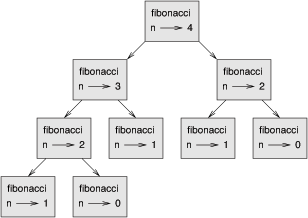
\includegraphics[scale=0.7]{../source/figs/fibonacci.pdf}}
\caption{Call graph.}
\label{fig.fibonacci}
\end{figure}

A call graph shows a set of function frames, with lines connecting each
frame to the frames of the functions it calls.  At the top of the
graph, {\tt fibonacci} with {\tt n=4} calls {\tt fibonacci} with {\tt
n=3} and {\tt n=2}.  In turn, {\tt fibonacci} with {\tt n=3} calls
{\tt fibonacci} with {\tt n=2} and {\tt n=1}.  And so on.
\index{function frame}
\index{frame}
\index{call graph}

Count how many times {\tt fibonacci(0)} and {\tt fibonacci(1)} are
called.  This is an inefficient solution to the problem, and it gets
worse as the argument gets bigger.
\index{memo}

One solution is to keep track of values that have already been
computed by storing them in a dictionary.  A previously computed value
that is stored for later use is called a {\bf memo}.  Here is a
``memoized'' version of {\tt fibonacci}:

\begin{verbatim}
known = {0:0, 1:1}

def fibonacci(n):
    if n in known:
        return known[n]

    res = fibonacci(n-1) + fibonacci(n-2)
    known[n] = res
    return res
\end{verbatim}
%
{\tt known} is a dictionary that keeps track of the Fibonacci
numbers we already know.  It starts with
two items: 0 maps to 0 and 1 maps to 1.

Whenever {\tt fibonacci} is called, it checks {\tt known}.
If the result is already there, it can return
immediately.  Otherwise it has to
compute the new value, add it to the dictionary, and return it.

If you run this version of {\tt fibonacci} and compare it with
the original, you will find that it is much faster.



\section{Global variables}
\index{global variable}
\index{variable!global}

In the previous example, {\tt known} is created outside the function,
so it belongs to the special frame called \verb"__main__".
Variables in \verb"__main__" are sometimes called {\bf global}
because they can be accessed from any function.  Unlike local
variables, which disappear when their function ends, global variables
persist from one function call to the next.
\index{flag}

It is common to use global variables for {\bf flags}; that is,
boolean variables that indicate (``flag'') whether a condition
is true.  For example, some programs use
a flag named {\tt verbose} to control the level of detail in the
output:

\begin{verbatim}
verbose = True

def example1():
    if verbose:
        print('Running example1')
\end{verbatim}
%
If you try to reassign a global variable, you might be surprised.
The following example is supposed to keep track of whether the
function has been called:
\index{reassignment}

\begin{verbatim}
been_called = False

def example2():
    been_called = True         # WRONG
\end{verbatim}
%
But if you run it you will see that the value of \verb"been_called"
doesn't change.  The problem is that {\tt example2} creates a new local
variable named \verb"been_called".  The local variable goes away when
the function ends, and has no effect on the global variable.
\index{global statement}
\index{statement!global}
\index{declaration}

To reassign a global variable inside a function you have to
{\bf declare} the global variable before you use it:

\begin{verbatim}
been_called = False

def example2():
    global been_called
    been_called = True
\end{verbatim}
%
The {\bf global statement} tells the interpreter
something like, ``In this function, when I say \verb"been_called", I
mean the global variable; don't create a local one.''
\index{update!global variable}
\index{global variable!update}

Here's an example that tries to update a global variable:

\begin{verbatim}
count = 0

def example3():
    count = count + 1          # WRONG
\end{verbatim}
%
If you run it you get:
\index{UnboundLocalError}
\index{exception!UnboundLocalError}

\begin{verbatim}
UnboundLocalError: local variable 'count' referenced before assignment
\end{verbatim}
%
Python assumes that {\tt count} is local, and under that assumption
you are reading it before writing it.  The solution, again,
is to declare {\tt count} global.
\index{counter}

\begin{verbatim}
def example3():
    global count
    count += 1
\end{verbatim}
%
If a global variable refers to a mutable value, you can modify
the value without declaring the variable:
\index{mutability}

\begin{verbatim}
known = {0:0, 1:1}

def example4():
    known[2] = 1
\end{verbatim}
%
So you can add, remove and replace elements of a global list or
dictionary, but if you want to reassign the variable, you
have to declare it:

\begin{verbatim}
def example5():
    global known
    known = dict()
\end{verbatim}
%
Global variables can be useful, but if you have a lot of them,
and you modify them frequently, they can make programs
hard to debug.


\section{Debugging}
\index{debugging}

As you work with bigger datasets it can become unwieldy to
debug by printing and checking the output by hand.  Here are some
suggestions for debugging large datasets:

\begin{description}

\item[Scale down the input:] If possible, reduce the size of the
dataset.  For example if the program reads a text file, start with
just the first 10 lines, or with the smallest example you can find.
You can either edit the files themselves, or (better) modify the
program so it reads only the first {\tt n} lines.

If there is an error, you can reduce {\tt n} to the smallest
value that manifests the error, and then increase it gradually
as you find and correct errors.

\item[Check summaries and types:] Instead of printing and checking the
entire dataset, consider printing summaries of the data: for example,
the number of items in a dictionary or the total of a list of numbers.

A common cause of runtime errors is a value that is not the right
type.  For debugging this kind of error, it is often enough to print
the type of a value.

\item[Write self-checks:]  Sometimes you can write code to check
for errors automatically.  For example, if you are computing the
average of a list of numbers, you could check that the result is
not greater than the largest element in the list or less than
the smallest.  This is called a ``sanity check'' because it detects
results that are ``insane''.
\index{sanity check}
\index{consistency check}

Another kind of check compares the results of two different
computations to see if they are consistent.  This is called a
``consistency check''.

\item[Format the output:] Formatting debugging output
can make it easier to spot an error.  We saw an example in
Section~\ref{factdebug}.  The {\tt pprint} module provides
a {\tt pprint} function that displays built-in types in
a more human-readable format ({\tt pprint} stands for
``pretty print'').
\index{pretty print}
\index{pprint module}
\index{module!pprint}

\end{description}

Again, time you spend building scaffolding can reduce
the time you spend debugging.
\index{scaffolding}


\section{Glossary}

\begin{description}

\item[mapping:] A relationship in which each element of one set
corresponds to an element of another set.
\index{mapping}

\item[dictionary:] A mapping from keys to their
corresponding values.
\index{dictionary}

\item[key-value pair:] The representation of the mapping from
a key to a value.
\index{key-value pair}

\item[item:] In a dictionary, another name for a key-value
  pair.
\index{item!dictionary}

\item[key:] An object that appears in a dictionary as the
first part of a key-value pair.
\index{key}

\item[value:] An object that appears in a dictionary as the
second part of a key-value pair.  This is more specific than
our previous use of the word ``value''.
\index{value}

\item[implementation:] A way of performing a computation.
\index{implementation}

\item[hashtable:] The algorithm used to implement Python
dictionaries.
\index{hashtable}

\item[hash function:] A function used by a hashtable to compute the
location for a key.
\index{hash function}

\item[hashable:] A type that has a hash function.  Immutable
types like integers,
floats and strings are hashable; mutable types like lists and
dictionaries are not.
\index{hashable}

\item[lookup:] A dictionary operation that takes a key and finds
the corresponding value.
\index{lookup}

\item[reverse lookup:] A dictionary operation that takes a value and finds
one or more keys that map to it.
\index{reverse lookup}

\item[raise statement:]  A statement that (deliberately) raises an exception.
\index{raise statement}
\index{statement!raise}

\item[singleton:] A list (or other sequence) with a single element.
\index{singleton}

\item[call graph:] A diagram that shows every frame created during
the execution of a program, with an arrow from each caller to
each callee.
\index{call graph}
\index{diagram!call graph}

\item[memo:] A computed value stored to avoid unnecessary future
computation.
\index{memo}

\item[global variable:]  A variable defined outside a function.  Global
variables can be accessed from any function.
\index{global variable}

\item[global statement:]  A statement that declares a variable name
global.
\index{global statement}
\index{statement!global}

\item[flag:] A boolean variable used to indicate whether a condition
is true.
\index{flag}

\item[declaration:] A statement like {\tt global} that tells the
interpreter something about a variable.
\index{declaration}

\end{description}


\section{Exercises}

\begin{exercise}
\label{wordlist2}
\index{set membership}
\index{membership!set}

Write a function that reads the words in {\tt words.txt} and
stores them as keys in a dictionary.  It doesn't matter what the
values are.  Then you can use the {\tt in} operator
as a fast way to check whether a string is in
the dictionary.

If you did Exercise~\ref{wordlist1}, you can compare the speed
of this implementation with the list {\tt in} operator and the
bisection search.

\end{exercise}


\begin{exercise}
\label{setdefault}

Read the documentation of the dictionary method {\tt setdefault}
and use it to write a more concise version of \verb"invert_dict".
Solution: \url{http://thinkpython2.com/code/invert_dict.py}.
\index{setdefault method}
\index{method!setdefault}

\end{exercise}


\begin{exercise}
Memoize the Ackermann function from Exercise~\ref{ackermann} and see if
memoization makes it possible to evaluate the function with bigger
arguments.  Hint: no.
Solution: \url{http://thinkpython2.com/code/ackermann_memo.py}.
\index{Ackermann function}
\index{function!ack}

\end{exercise}



\begin{exercise}
\index{duplicate}

If you did Exercise~\ref{duplicate}, you already have
a function named \verb"has_duplicates" that takes a list
as a parameter and returns {\tt True} if there is any object
that appears more than once in the list.

Use a dictionary to write a faster, simpler version of
\verb"has_duplicates".
Solution: \url{http://thinkpython2.com/code/has_duplicates.py}.

\end{exercise}


\begin{exercise}
\label{exrotatepairs}
\index{letter rotation}
\index{rotation!letters}

Two words are ``rotate pairs'' if you can rotate one of them
and get the other (see \verb"rotate_word" in Exercise~\ref{exrotate}).

Write a program that reads a wordlist and finds all the rotate
pairs.  Solution: \url{http://thinkpython2.com/code/rotate_pairs.py}.

\end{exercise}


\begin{exercise}
\index{Car Talk}
\index{Puzzler}

Here's another Puzzler from {\em Car Talk}
(\url{http://www.cartalk.com/content/puzzlers}):

\begin{quote}
This was sent in by a fellow named Dan O'Leary. He came upon a common
one-syllable, five-letter word recently that has the following unique
property. When you remove the first letter, the remaining letters form
a homophone of the original word, that is a word that sounds exactly
the same. Replace the first letter, that is, put it back and remove
the second letter and the result is yet another homophone of the
original word. And the question is, what's the word?

Now I'm going to give you an example that doesn't work. Let's look at
the five-letter word, `wrack.' W-R-A-C-K, you know like to `wrack with
pain.' If I remove the first letter, I am left with a four-letter
word, 'R-A-C-K.' As in, `Holy cow, did you see the rack on that buck!
It must have been a nine-pointer!' It's a perfect homophone. If you
put the `w' back, and remove the `r,' instead, you're left with the
word, `wack,' which is a real word, it's just not a homophone of the
other two words.

But there is, however, at least one word that Dan and we know of,
which will yield two homophones if you remove either of the first two
letters to make two, new four-letter words. The question is, what's
the word?
\end{quote}
\index{homophone}
\index{reducible word}
\index{word, reducible}

You can use the dictionary from Exercise~\ref{wordlist2} to check
whether a string is in the word list.

To check whether two words are homophones, you can use the CMU
Pronouncing Dictionary.  You can download it from
\url{http://www.speech.cs.cmu.edu/cgi-bin/cmudict} or from
\url{http://thinkpython2.com/code/c06d} and you can also download
\url{http://thinkpython2.com/code/pronounce.py}, which provides a function
named \verb"read_dictionary" that reads the pronouncing dictionary and
returns a Python dictionary that maps from each word to a string that
describes its primary pronunciation.

Write a program that lists all the words that solve the Puzzler.
Solution: \url{http://thinkpython2.com/code/homophone.py}.

\end{exercise}


\chapter{Tuples | 元组}
\label{tuplechap}

This chapter presents one more built-in type, the tuple, and then
shows how lists, dictionaries, and tuples work together.
I also present a useful feature for variable-length argument lists,
the gather and scatter operators.

One note: there is no consensus on how to pronounce ``tuple''.
Some people say ``tuh-ple'', which rhymes with ``supple''.  But
in the context of programming, most people say ``too-ple'', which
rhymes with ``quadruple''.

本章介绍另一个内建的类型 --- 元组\footnote{值得注意的是,``tuple''并没有统一的发音,有些人读``tuh-ple'',音律类似于``supple'';而有人读``too-ple''音律类似于``quadruple''。},同时向您展示列表、字典和元组如何结合使用。后面的章节也会展示关于可变长度参数列表的有用功能,以及\emph{汇集}和\emph{离散}操作。

\section{Tuples are immutable | 元组的不可变性}
\index{tuple}
\index{type!tuple}
\index{sequence}

A tuple is a sequence of values.  The values can be any type, and
they are indexed by integers, so in that respect tuples are a lot
like lists.  The important difference is that tuples are immutable.
\index{mutability}
\index{immutability}

元组是一组\emph{值}的序列。  其中的值可以是任意类型,使用整数索引其位置,因此元组与列表非常相似。  而重要的不同之处在于元组的不可变性。

Syntactically, a tuple is a comma-separated list of values:

语法上,元组是用逗号隔开的值的列表:

\begin{lstlisting}
>>> t = 'a', 'b', 'c', 'd', 'e'
\end{lstlisting}
%
Although it is not necessary, it is common to enclose tuples in
parentheses:

尽管不是必须,通常我们在给元组赋值时会用括号把元素封装起来:

\index{parentheses!tuples in}

\begin{lstlisting}
>>> t = ('a', 'b', 'c', 'd', 'e')
\end{lstlisting}
%
To create a tuple with a single element, you have to include a final
comma:

使用单一元素建立元组时,需要在结尾使用一个逗号:

\index{singleton}
\index{tuple!singleton}

\begin{lstlisting}
>>> t1 = 'a',
>>> type(t1)
<class 'tuple'>
\end{lstlisting}
%
A value in parentheses is not a tuple:

括号中仅包含元素(而没有使用逗号结尾)时被赋值的对象不是元组:

\begin{lstlisting}
>>> t2 = ('a')
>>> type(t2)
<class 'str'>
\end{lstlisting}
%
Another way to create a tuple is the built-in function {\tt tuple}.
With no argument, it creates an empty tuple:
\index{tuple function}
\index{function!tuple}

另一个建立元组的方法是使用内建函数 \lstinline{tuple}。 在没有参数传递时它会产生一个空元组。

\begin{lstlisting}
>>> t = tuple()
>>> t
()
\end{lstlisting}

%
If the argument is a sequence (string, list or tuple), the result
is a tuple with the elements of the sequence:



\begin{verbatim}
>>> t = tuple('lupins')
>>> t
('l', 'u', 'p', 'i', 'n', 's')
\end{verbatim}
%
Because {\tt tuple} is the name of a built-in function, you should
avoid using it as a variable name.

因为\lstinline{tuple}是内建函数名,所以应该避免将它用于变量名。


Most list operators also work on tuples.  The bracket operator
indexes an element:

列表的大多数操作同样也适用于元组。 例如使用方括号索引一个元素:

\index{bracket operator}
\index{operator!bracket}

\begin{lstlisting}
>>> t = ('a', 'b', 'c', 'd', 'e')
>>> t[0]
'a'
\end{lstlisting}
%
And the slice operator selects a range of elements.

切片操作可以选取一个范围内的元素:
\index{slice operator}
\index{operator!slice}
\index{tuple!slice}
\index{slice!tuple}

\begin{lstlisting}
>>> t[1:3]
('b', 'c')
\end{lstlisting}
%
But if you try to modify one of the elements of the tuple, you get
an error:

但是,如果你试图元组中的一个元素,会得到错误信息:

\index{exception!TypeError}
\index{TypeError}
\index{item assignment}
\index{assignment!item}

\begin{lstlisting}
>>> t[0] = 'A'
TypeError: object doesn't support item assignment
\end{lstlisting}
%
Because tuples are immutable, you can't modify the elements.  But you
can replace one tuple with another:

因为元组是不可变的,您无法改变其中的元素。 但是您可以使用其他元组替换现有元组:

\begin{lstlisting}
>>> t = ('A',) + t[1:]
>>> t
('A', 'b', 'c', 'd', 'e')
\end{lstlisting}
%
This statement makes a new tuple and then makes {\tt t} refer to it.

这个语句产生了一个新元组,并且将它赋给了原先的元组\lstinline{t}。

The relational operators work with tuples and other sequences;
Python starts by comparing the first element from each
sequence.  If they are equal, it goes on to the next elements,
and so on, until it finds elements that differ.  Subsequent
elements are not considered (even if they are really big).

关系型操作也适用于元组和其他序列;Python 会首先比较序列中的第一个元素,如果它们相同就会去比较下一组元素,以此往复,直至比值不同。 其后的元素(即便是差异很大)也不会再参与比较。

\index{comparison!tuple}
\index{tuple!comparison}

\begin{lstlisting}
>>> (0, 1, 2) < (0, 3, 4)
True
>>> (0, 1, 2000000) < (0, 3, 4)
True
\end{lstlisting}


\section{Tuple assignment | 元组赋值}
\label{tuple.assignment} \index{tuple!assignment} \index{assignment!tuple}
\index{swap pattern} \index{pattern!swap}

It is often useful to swap the values of two variables.
With conventional assignments, you have to use a temporary
variable.  For example, to swap {\tt a} and {\tt b}:

两个变量互换值的操作通常很有用。 传统的,你需要使用一个临时变量。 例如为了交换\lstinline{a}和\lstinline{b}:

\begin{lstlisting}
>>> temp = a
>>> a = b
>>> b = temp
\end{lstlisting}
%
This solution is cumbersome; {\bf tuple assignment} is more elegant:

这个方法很繁琐;通过{\bf 元组赋值}的来实现更为优雅:

\begin{lstlisting}
>>> a, b = b, a
\end{lstlisting}
%
The left side is a tuple of variables; the right side is a tuple of
expressions.  Each value is assigned to its respective variable.
All the expressions on the right side are evaluated before any
of the assignments.

等号左侧是变量构成的元组;右侧是元组赋值的表达式。  每个值都被赋给了对应的要互换的变量。  变量被重新赋值前,右侧的表达式会被优先运行。

The number of variables on the left and the number of
values on the right have to be the same:

使用元组赋值,左右的变量数必须相同:

\index{exception!ValueError}
\index{ValueError}

\begin{lstlisting}
>>> a, b = 1, 2, 3
ValueError: too many values to unpack
\end{lstlisting}
%
More generally, the right side can be any kind of sequence
(string, list or tuple).  For example, to split an email address
into a user name and a domain, you could write:

一般说来,元组赋值的右侧表达式可以是任意类型(字符串、列表或者元组)的序列。 例如, 将一个电子邮箱地址分成用户名和域名, 你可以:

\index{split method}
\index{method!split}
\index{email address}

\begin{lstlisting}
>>> addr = 'monty@python.org'
>>> uname, domain = addr.split('@')
\end{lstlisting}
%
The return value from {\tt split} is a list with two elements;
the first element is assigned to {\tt uname}, the second to
{\tt domain}.

\lstinline{split}函数返回的对象是一个包含两个元素的列表;第一个元素被赋给了\lstinline{uname}的变量,第二个被赋给了\lstinline{domain}。

\begin{lstlisting}
>>> uname
'monty'
>>> domain
'python.org'
\end{lstlisting}
%

\section{Tuples as return values | 元组作为返回值}
\index{tuple} \index{value!tuple} \index{return value!tuple}
\index{function, tuple as return value}

Strictly speaking, a function can only return one value, but
if the value is a tuple, the effect is the same as returning
multiple values.  For example, if you want to divide two integers
and compute the quotient and remainder, it is inefficient to
compute {\tt x/y} and then {\tt x\%y}.  It is better to compute
them both at the same time.

严格地说,一个函数只能返回一个值,但是如果以元组作为这个返回值,其效果等同于返回多个值。 例如,你想对两个整数做除法,计算出商和余数,依次计算出\lstinline{x/y}和\lstinline{x%y}是很低效的。 更好的方法就是同时计算出它们。
\index{divmod}

The built-in function {\tt divmod} takes two arguments and
returns a tuple of two values, the quotient and remainder.
You can store the result as a tuple:

内建函数\href{https://docs.python.org/3/library/functions.html#divmod}{\lstinline{divmod}}接受两个参数,返回包含两个值的元组 --- 输入参数做除法的商和余数。 您可以使用元组来存储返回值:

\begin{lstlisting}
>>> t = divmod(7, 3)
>>> t
(2, 1)
\end{lstlisting}
%
Or use tuple assignment to store the elements separately:

或者使用元组赋值分别存储它们:

\index{tuple assignment}
\index{assignment!tuple}

\begin{lstlisting}
>>> quot, rem = divmod(7, 3)
>>> quot
2
>>> rem
1
\end{lstlisting}
%
Here is an example of a function that returns a tuple:

下面是另一个返回元组作为结果的函数例子:

\begin{lstlisting}
def min_max(t):
    return min(t), max(t)
\end{lstlisting}
%
{\tt max} and {\tt min} are built-in functions that find
the largest and smallest elements of a sequence.  \verb"min_max"
computes both and returns a tuple of two values.

\lstinline{max} 和 \lstinline{min} 是用于找出一组元素序列中最大值和最小值的内建函数,\lstinline{min_max}函数同时计算出它们并组装成元组返回结果。
\index{max function} \index{function!max}
\index{min function} \index{function!min}


\section{Variable-length argument tuples | 可变长度参数元组}
\label{gather}
\index{variable-length argument tuple} \index{argument!variable-length tuple}
\index{gather} \index{parameter!gather} \index{argument!gather}

Functions can take a variable number of arguments.  A parameter
name that begins with {\tt *} {\bf gathers} arguments into
a tuple.  For example, {\tt printall}
takes any number of arguments and prints them:

函数可以同时接受多个参数。 以 {\bf *} 开头的定义参数可以将输入的参数 \emph{汇集}到一个元组中。 例如 \lstinline{printall} 可以接受任意数量的参数,并且打印出来:

\begin{lstlisting}
def printall(*args):
    print(args)
\end{lstlisting}
%
The gather parameter can have any name you like, but {\tt args} is
conventional.  Here's how the function works:

汇集的形参可以使用任意名字, 传统上使用\lstinline{args}. 以下显示了这个函数的调用效果:

\begin{lstlisting}
>>> printall(1, 2.0, '3')
(1, 2.0, '3')
\end{lstlisting}
%
The complement of gather is {\bf scatter}.  If you have a
sequence of values and you want to pass it to a function
as multiple arguments, you can use the {\tt *} operator.
For example, {\tt divmod} takes exactly two arguments; it
doesn't work with a tuple:

\emph{离散}{\bf scatter}是汇集的补充。 如果你有一个值的序列,并且希望
将其作为多个参数传递给一个函数,你可以使用运算符\lstinline{*}。
例如,\lstinline{divmod} 需要接受两个实参;一个元组则无法作为参数传递进去:

\index{scatter} \index{argument scatter} \index{TypeError}
\index{exception!TypeError}

\begin{lstlisting}
>>> t = (7, 3)
>>> divmod(t)
TypeError: divmod expected 2 arguments, got 1
\end{lstlisting}
%
But if you scatter the tuple, it works:

但是如果您将这个元组打散,它就可以被传递进函数:

\begin{lstlisting}
>>> divmod(*t)
(2, 1)
\end{lstlisting}

%
Many of the built-in functions use
variable-length argument tuples.  For example, {\tt max}
and {\tt min} can take any number of arguments:

多数内建函数使用可变长度参数元组。 例如,\lstinline{max} 和 \lstinline{min} 可以取任意数量的参数。

\index{max function} \index{function!max}
\index{min function} \index{function!min}

\begin{lstlisting}
>>> max(1, 2, 3)
3
\end{lstlisting}
%
But {\tt sum} does not.

但是求和操作\lstinline{sum}并不如此:
\index{sum function} \index{function!sum}

\begin{lstlisting}
>>> sum(1, 2, 3)
TypeError: sum expected at most 2 arguments, got 3
\end{lstlisting}
%
As an exercise, write a function called {\tt sumall} that takes any number
of arguments and returns their sum.

您可以尝试写一个叫做 \lstinline{sumall}的函数作为练习,使它能够接受任何数量的传参并返回它们的和。

\section{Lists and tuples | 列表和元组}
\index{zip function} \index{function!zip}

{\tt zip} is a built-in function that takes two or more sequences and
returns a list of tuples where each tuple contains one
element from each sequence.  The name of the function refers to
a zipper, which joins and interleaves two rows of teeth.

\lstinline{zip} 是一个内建函数,用于将两个或多个序列组装成包含元组的列表返回出来,每个元组包含了各个序列中相对位置的一个元素。这个函数的起名来源于名词拉链(zipper),形象的显示年对应两列对应位置的牙齿组合起来。

This example zips a string and a list:

下面例子显示了组合字符串和列表操作:

\begin{lstlisting}
>>> s = 'abc'
>>> t = [0, 1, 2]
>>> zip(s, t)
<zip object at 0x7f7d0a9e7c48>
\end{lstlisting}
%
The result is a {\bf zip object} that knows how to iterate through
the pairs.  The most common use of {\tt zip} is in a {\tt for} loop:

输出的结果是一个可以通过每个内在的元组对进行迭代的 \lstinline{zip} 对象。 \lstinline{zip}函数最常见用法就是基于\lstinline{for}循环的迭代遍历:

\begin{lstlisting}
>>> for pair in zip(s, t):
...     print(pair)
...
('a', 0)
('b', 1)
('c', 2)
\end{lstlisting}

%
A zip object is a kind of {\bf iterator}, which is any object
that iterates through a sequence.  Iterators are similar to lists in some
ways, but unlike lists, you can't use an index to select an element from
an iterator.

\href{https://docs.python.org/3/library/functions.html#zip}{\lstinline{zip}}对象是一个友善的\textbf{迭代器},后者是指任何一种能够按照某个序列迭代的对象。 迭代器在某些方面与列表非常相似, 不同之处在于你无法通过索引来选择迭代器中的某个元素。
\index{iterator} \index{迭代器}

If you want to use list operators and methods, you can
use a zip object to make a list:

如果你想对\lstinline {zip}对象使用列表的操作和方法,你可以通过\lstinline {zip}对象创造一个列表:

\begin{lstlisting}
>>> list(zip(s, t))
[('a', 0), ('b', 1), ('c', 2)]
\end{lstlisting}

%
The result is a list of tuples; in this example, each tuple contains
a character from the string and the corresponding element from
the list.

结果就是产生了一个包含若干元组的列表;在这个例子中,每个元组又包含了字符串中的一个字符和列表\lstinline {t} 中对应的一个元素。
\index{list!of tuples}

If the sequences are not the same length, the result has the
length of the shorter one.

如果用于创建\lstinline{zip}的序列长度不一,返回的对象的长度以最短序列的长度为准。

\begin{lstlisting}
>>> list(zip('Anne', 'Elk'))
[('A', 'E'), ('n', 'l'), ('n', 'k')]
\end{lstlisting}
%
You can use tuple assignment in a {\tt for} loop to traverse a list of
tuples:

您可以通过元组赋值在\lstinline{for}循环中遍历包含元组的列表:
\index{traversal} \index{tuple assignment} \index{assignment!tuple}

\begin{lstlisting}
t = [('a', 0), ('b', 1), ('c', 2)]
for letter, number in t:
    print(number, letter)
\end{lstlisting}
%
Each time through the loop, Python selects the next tuple in
the list and assigns the elements to {\tt letter} and
{\tt number}.  The output of this loop is:

循环中的每次执行, Python 会选择列表中的下一个元组,并将其内容赋给 \lstinline{letter} 和 \lstinline{number}。因此循环打印的输出会是这样:
\index{loop}

\begin{lstlisting}
0 a
1 b
2 c
\end{lstlisting}

%
If you combine {\tt zip}, {\tt for} and tuple assignment, you get a
useful idiom for traversing two (or more) sequences at the same
time.  For example, \verb"has_match" takes two sequences, {\tt t1} and
{\tt t2}, and returns {\tt True} if there is an index {\tt i}
such that {\tt t1[i] == t2[i]}:

如果将\lstinline{zip}、\lstinline{for}和元组赋值结合起来使用,您会得出一个有用的惯用方法用于
同时遍历两个(甚至多个)序列。 如下例,\lstinline{has_match} 接受两个序列,\lstinline{t1}和\lstinline{t2},并返回一个真值\lstinline{True}如果存在满足判别式 \lstinline{t1[i] == t2[i]}的索引\lstinline {i}:
\index{for loop}

\begin{lstlisting}
def has_match(t1, t2):
    for x, y in zip(t1, t2):
        if x == y:
            return True
    return False
\end{lstlisting}

%
If you need to traverse the elements of a sequence and their
indices, you can use the built-in function {\tt enumerate}:

如果需要遍历一个序列的元素以及它们的索引号,您可以使用内建函数\lstinline{enumerate}:
\index{traversal} \index{enumerate function} \index{function!enumerate}

\begin{lstlisting}
for index, element in enumerate('abc'):
    print(index, element)
\end{lstlisting}

%
The result from {\tt enumerate} is an enumerate object, which
iterates a sequence of pairs; each pair contains an index (starting
from 0) and an element from the given sequence.
In this example, the output is

\lstinline{enumerate}的返回结果是一个枚举对象(enumerate object),它可基于一个包含若干个\emph{对}的序列进行迭代,每个对包含了(从0开始计数)的索引号和对应的元素。在刚才的例子中,对应的输出结果会和上次一样:

\begin{lstlisting}
0 a
1 b
2 c
\end{lstlisting}

%
Again.
\index{iterator}    \index{object!enumerate}    \index{enumerate object}


\section{Dictionaries and tuples | 字典和元组}
\label{dictuple}
\index{dictionary} \index{items method}
\index{method!items} \index{key-value pair}

Dictionaries have a method called {\tt items} that returns a sequence of
tuples, where each tuple is a key-value pair.

字典对象有一个内建方法叫做\href{https://docs.python.org/3/library/stdtypes.html?highlight=items#dict.items}{\lstinline{itmes}}, 它返回一个以元组形式存放的键-值对的序列。

\begin{lstlisting}
>>> d = {'a':0, 'b':1, 'c':2}
>>> t = d.items()
>>> t
dict_items([('c', 2), ('a', 0), ('b', 1)])
\end{lstlisting}
%
The result is a \verb"dict_items" object, which is an iterator that
iterates the key-value pairs.  You can use it in a {\tt for} loop
like this:

其结果是一个\lstinline{dict_itmes}对象,其实质是一个可以通过键-值对迭代的迭代器。 您可以在\lstinline{for}循环中像这样使用它:
\index{iterator}

\begin{lstlisting}
>>> for key, value in d.items():
...     print(key, value)
...
c 2
a 0
b 1
\end{lstlisting}
%
As you should expect from a dictionary, the items are in no
particular order.

和字典对象相似,\lstinline{dict_itmes}内部的项是无序存放的。

Going in the other direction, you can use a list of tuples to
initialize a new dictionary:

另一方面,您可以使用元组的列表初始化一个新的字典:
\index{dictionary!initialize}

\begin{lstlisting}
>>> t = [('a', 0), ('c', 2), ('b', 1)]
>>> d = dict(t)
>>> d
{'a': 0, 'c': 2, 'b': 1}
\end{lstlisting}

Combining {\tt dict} with {\tt zip} yields a concise way
to create a dictionary:

\lstinline{dict}和\lstinline{zip}的结合使用产生了一个简洁的字典生成法:
\index{zip function!use with dict}

\begin{lstlisting}
>>> d = dict(zip('abc', range(3)))
>>> d
{'a': 0, 'c': 2, 'b': 1}
\end{lstlisting}
%
The dictionary method {\tt update} also takes a list of tuples
and adds them, as key-value pairs, to an existing dictionary.


字典的\lstinline{update}方法也接受元组的列表,并作为键-值对把它们加入到该字典中去。
\index{update method} \index{method!update} \index{traverse!dictionary}
\index{dictionary!traversal}

It is common to use tuples as keys in dictionaries (primarily because
you can't use lists).  For example, a telephone directory might map
from last-name, first-name pairs to telephone numbers.  Assuming
that we have defined {\tt last}, {\tt first} and {\tt number}, we
could write:

更加常用的方法是在字典中使用元组作为键(因为列表做不了键)。例如,一个电话簿希望基于用户的姓(\lstinline {last})、名(\lstinline {first})对来映射号码(\lstinline {number}),假设我们已经定义了 \lstinline {last}, \lstinline {first} 和 \lstinline {number}三个变量,我们可以这样实现映射:
\index{tuple!as key in dictionary}
\index{hashable}

\begin{lstlisting}
directory[last, first] = number
\end{lstlisting}
%
The expression in brackets is a tuple.  We could use tuple
assignment to traverse this dictionary.

方括号中的表达式是一个元组。 为我们可以通过元组赋值来遍历这个字典:
\index{tuple!in brackets}

\begin{lstlisting}
for last, first in directory:
    print(first, last, directory[last,first])
\end{lstlisting}

%
This loop traverses the keys in {\tt directory}, which are tuples.  It
assigns the elements of each tuple to {\tt last} and {\tt first}, then
prints the name and corresponding telephone number.

该循环遍历\lstinline{directory}中的键,它们其实是元组。
它将元组的元素赋给\lstinline{last}和\lstinline{first}, 然后打印出姓名和对应的电话号码。

There are two ways to represent tuples in a state diagram.  The more
detailed version shows the indices and elements just as they appear in
a list.  For example, the tuple \verb"('Cleese', 'John')" would appear
as in Figure~\ref{fig.tuple1}.

用两个状态图来表述这些元组。细致的说,索引号和对应元素就像列表一样存放在元组中。例如,元组\lstinline{('Cleese', 'John')}可像图~\ref{fig.tuple1}一样存放。
\index{state diagram} \index{diagram!state}

\begin{figure}
\centerline
{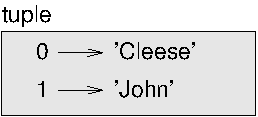
\includegraphics[scale=0.8]{figs/tuple1.pdf}}
\caption{State diagram.}
\label{fig.tuple1}
\end{figure}

But in a larger diagram you might want to leave out the
details.  For example, a diagram of the telephone directory might
appear as in Figure~\ref{fig.dict2}.

在大图中,我们忽略这些细节。 该电话簿的结构图可能像图~\ref{fig.dict2}一样。

\begin{figure}
\centerline
{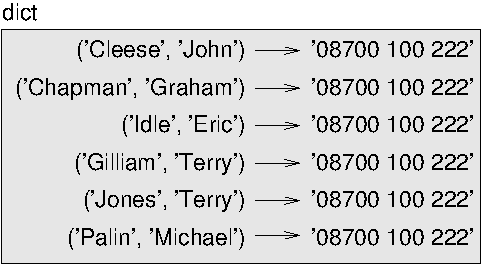
\includegraphics[scale=0.8]{figs/dict2.pdf}}
\caption{State diagram.}
\label{fig.dict2}
\end{figure}

Here the tuples are shown using Python syntax as a graphical
shorthand.  The telephone number in the diagram is the complaints line
for the BBC, so please don't call it.

因此,Python风格的元组用法可用这两幅图来描述。 此图中的电话号码是BBC的投诉热线,请不要拨打它。


\section{Sequences of sequences | 序列嵌套}
\index{sequence}

I have focused on lists of tuples, but almost all of the examples in
this chapter also work with lists of lists, tuples of tuples, and
tuples of lists.  To avoid enumerating the possible combinations, it
is sometimes easier to talk about sequences of sequences.

我们已经谈过了包含元组的列表,事实上,本章大多数例子也适用于列表嵌套列表、元组嵌套元组,以及元组嵌套列表。 为了避免一一穷举这类可能的嵌套组合,我们简称为序列嵌套。

In many contexts, the different kinds of sequences (strings, lists and
tuples) can be used interchangeably.  So how should you choose one
over the others?

在很多情况下,不同类型的序列(字符串、列表、元组)可以互换使用。 因此,我们如何选用合适的嵌套对象呢?
\index{string} \index{list} \index{tuple} \index{mutability}
\index{immutability}

To start with the obvious, strings are more limited than other
sequences because the elements have to be characters.  They are
also immutable.  If you need the ability to change the characters
in a string (as opposed to creating a new string), you might
want to use a list of characters instead.

首先,显而易见的是字符串的使用范围比其他序列更为有限,因为它的所有元素都是字符,且字符串不可变。如果你希望能够改变字符在字符串中的位置,使用列表嵌套字符比较合适。

Lists are more common than tuples, mostly because they are mutable.
But there are a few cases where you might prefer tuples:

列表比元组更常见,这源于它们可变性的易用。  但是有些情况下我们不得不更青睐元组:

\begin{enumerate}

\item In some contexts, like a {\tt return} statement, it is
syntactically simpler to create a tuple than a list.

\item If you want to use a sequence as a dictionary key, you
have to use an immutable type like a tuple or string.

\item If you are passing a sequence as an argument to a function,
using tuples reduces the potential for unexpected behavior
due to aliasing.

\end{enumerate}

\begin{enumerate}

\item 在一些情况下(例如\lstinline{return}语句),从句式上生成一个元组比列表要简单。

\item 如果你想使用一个序列作为字典的键,那么你必须使用元组或字符串这样的不可变类型。

\item 如果你向函数传入一个序列作为参数,那么使用元组以降低由于别名而产生的意外行为的可能性。

\end{enumerate}

Because tuples are immutable, they don't provide methods like {\tt
  sort} and {\tt reverse}, which modify existing lists.  But Python
provides the built-in function {\tt sorted}, which takes any sequence
and returns a new list with the same elements in sorted order, and
{\tt reversed}, which takes a sequence and returns an iterator that
traverses the list in reverse order.

正由于元组的不可变性,元组没有类似于列表中的 \lstinline{sort} (\emph{排序}) 和 \lstinline{reverser} (\emph{逆序})这样的方法。  然而 Python 提供了内建函数 \lstinline{sorted},用于对任意序列排序并输出相同元素的列表,以及 \lstinline {reversed},用于对序列逆向排序并生成一个可以遍历的迭代器。

\index{sorted function} \index{function!sorted} \index{reversed function}
\index{function!reversed} \index{iterator}


\section{Debugging  |  调试}
\index{debugging} \index{data structure}
\index{shape error} \index{error!shape}

Lists, dictionaries and tuples are examples of {\bf data
  structures}; in this chapter we are starting to see compound data
structures, like lists of tuples, or dictionaries that contain tuples
as keys and lists as values.  Compound data structures are useful, but
they are prone to what I call {\bf shape errors}; that is, errors
caused when a data structure has the wrong type, size, or structure.
For example, if you are expecting a list with one integer and I
give you a plain old integer (not in a list), it won't work.

列表、字典和元组都是\emph{数据结构} (\textbf{data structures})的实例;本章中我们开始接触到复合数据结构(\textbf{compound data structures}),如:列表嵌套元组,又如使用元组作为键而列表作为值的字典。复合数据结构非常实用,然而使用时容易出现所谓的\emph{形状错误}(\textbf{shape errors}),也就是说由于数据结构的类型、大小或结构问题而引发的错误。例如,当你希望使用封装整数的列表时却用成了没被列表包含的一串整数。
\index{structshape module} \index{module!structshape}

To help debug these kinds of errors, I have written a module
called {\tt structshape} that provides a function, also called
{\tt structshape}, that takes any kind of data structure as
an argument and returns a string that summarizes its shape.
You can download it from \url{http://thinkpython2.com/code/structshape.py}

为了方面调试这类错误,笔者编写了一个叫做 \lstinline{structshape} 的模块, 它提供了一个名为 \lstinline{structshape}的函数,用于接受并分析数据结构对象作,并返回描述它形状的文字信息。你可以在\href{http://thinkpython2.com/code/structshape.py}{此处}下载到它(\url{http://thinkpython2.com/code/structshape.py})。

Here's the result for a simple list:

这里是它分析简单列表的结果展示:

\begin{lstlisting}
>>> from structshape import structshape
>>> t = [1, 2, 3]
>>> structshape(t)
'list of 3 int'
\end{lstlisting}
%
A fancier program might write ``list of 3 int{\em s}'', but it
was easier not to deal with plurals.  Here's a list of lists:

更完美的程序应该显示 ``list of 3 int{\em s}'',但是忽略英文复数使程序简单的多。我们再看一个列表嵌套的例子:

\begin{lstlisting}
>>> t2 = [[1,2], [3,4], [5,6]]
>>> structshape(t2)
'list of 3 list of 2 int'
\end{lstlisting}
%
If the elements of the list are not the same type,
{\tt structshape} groups them, in order, by type:

如果列表内嵌套的元素不是相同类型,\lstinline{structshape} 会按类型的组将它们归并:

\begin{lstlisting}
>>> t3 = [1, 2, 3, 4.0, '5', '6', [7], [8], 9]
>>> structshape(t3)
'list of (3 int, float, 2 str, 2 list of int, int)'
\end{lstlisting}
%
Here's a list of tuples:

以下是一个元组的例子:

\begin{lstlisting}
>>> s = 'abc'
>>> lt = list(zip(t, s))
>>> structshape(lt)
'list of 3 tuple of (int, str)'
\end{lstlisting}
%
And here's a dictionary with 3 items that map integers to strings.

下面,一个包含3个映射整数到字符串的键值对的字典被分析:

\begin{lstlisting}
>>> d = dict(lt)
>>> structshape(d)
'dict of 3 int->str'
\end{lstlisting}
%
If you are having trouble keeping track of your data structures,
{\tt structshape} can help.

因此如果你对使用的数据结构有疑惑,可以使用\lstinline{structshape}来帮助解析。

\section{Glossary  |  术语表}

\begin{description}

\item[tuple:] An immutable sequence of elements.

\item[元组:] 一组不可变的元素的序列。
\index{tuple}

\item[tuple assignment:] An assignment with a sequence on the
right side and a tuple of variables on the left.  The right
side is evaluated and then its elements are assigned to the
variables on the left.

\item[元组赋值:]一种通过赋值方式,通过等号右侧的序列向等号左侧的一组变量的元组进行赋值。右侧许两种的每个元素会被计算,然后赋给左侧元组中对应的变量。
\index{tuple assignment} \index{assignment!tuple}

\item[gather:] The operation of assembling a variable-length
argument tuple.
\index{gather}

\item[汇集:] 组装可变长度变量元组的一种操作。

\item[scatter:] The operation of treating a sequence as a list of
arguments.
\index{scatter}

\item[分散:] 将一个序列变换成一个参数列表的操作。


\item[zip object:] The result of calling a built-in function {\tt zip};
an object that iterates through a sequence of tuples.

\item[zip 对象:] 使用内建函数\lstinline{zip}所返回的结果, 它是一个可通过元组序列逐个迭代的对象。
\index{zip object} \index{object!zip}

\item[iterator:] An object that can iterate through a sequence, but
which does not provide list operators and methods.

\item[迭代器:]: 一种可以通过一个序列逐个迭代的对象,但是它并不提供列表的某些操作和方法。
\index{iterator}

\item[data structure:] A collection of related values, often
organized in lists, dictionaries, tuples, etc.

\item[数据结构:] 一个有相关关联的数据的集合,通常使用列表、字典和元组等综合构成。
\index{data structure}

\item[shape error:] An error caused because a value has the
wrong shape; that is, the wrong type or size.

\item[形状错误:] 由于数据结构的类型、大小或结构问题而引发的错误。
\index{shape}

\end{description}


\section{Exercises  |  练习}

\begin{exercise}

Write a function called \verb"most_frequent" that takes a string and
prints the letters in decreasing order of frequency.  Find text
samples from several different languages and see how letter frequency
varies between languages.  Compare your results with the tables at
\url{http://en.wikipedia.org/wiki/Letter_frequencies}.  Solution:
\url{http://thinkpython2.com/code/most_frequent.py}.

写一个名为\emph{\lstinline{most_frequent}}的函数,它接受字符串并按字母降序打印出字符出现频率。 找一些不同语言的文本样本来试试看不同语言文本间区别。 将你的结果和维基百科上\href{http://en.wikipedia.org/wiki/Letter_frequencies}{字母频率}表相比较。

\href{http://thinkpython2.com/code/most_frequent.py}{参考答案}
\index{letter frequency} \index{frequency!letter}
\end{exercise}


\begin{exercise}
\label{anagrams}
\index{anagram set}
\index{set!anagram}

More anagrams!

\begin{enumerate}

\item Write a program
that reads a word list from a file (see Section~\ref{wordlist}) and
prints all the sets of words that are anagrams.

Here is an example of what the output might look like:

\begin{lstlisting}
['deltas', 'desalt', 'lasted', 'salted', 'slated', 'staled']
['retainers', 'ternaries']
['generating', 'greatening']
['resmelts', 'smelters', 'termless']
\end{lstlisting}

%
Hint: you might want to build a dictionary that maps from a
collection of letters to a list of words that can be spelled with those
letters.  The question is, how can you represent the collection of
letters in a way that can be used as a key?

\item Modify the previous program so that it prints the longest list
of anagrams first, followed by the second longest, and so on.
\index{Scrabble}
\index{bingo}

\item In Scrabble a ``bingo'' is when you play all seven tiles in
your rack, along with a letter on the board, to form an eight-letter
word.  What collection of 8 letters forms the most possible bingos?
Hint: there are seven.

% (7, ['angriest', 'astringe', 'ganister', 'gantries', 'granites',
% 'ingrates', 'rangiest'])

Solution: \url{http://thinkpython2.com/code/anagram_sets.py}.


易位构词游戏 (\href{https://zh.wikipedia.org/wiki/%E6%98%93%E4%BD%8D%E6%9E%84%E8%AF%8D%E6%B8%B8%E6%88%8F}{anagrams})!

\item 编写一个程序使之能从文件以列表形式读入单词 (参考章节~\ref{wordlist}) 并且打印出所有符合异位构词的组合。

下面是一个输出异位构词的样例:

\begin{lstlisting}
['deltas', 'desalt', 'lasted', 'salted', 'slated', 'staled']
['retainers', 'ternaries']
['generating', 'greatening']
['resmelts', 'smelters', 'termless']
\end{lstlisting}

提示:也许你可以建立一个字典用于映射一个字符集合到一个该集合可异位构词的词汇集合。

\item 改写前面的程序,使之首先打印包含异位构词数量最多的词汇列表,第二多次之,依次按异位构词数量排列。

\item \href{https://en.wikipedia.org/wiki/Scrabble}{Scrabble} \href{https://zh.wikipedia.org/wiki/Scrabble}{游戏} 中, “bingo” ...

\href{http://thinkpython2.com/code/anagram_sets.py}{参考答案}

\end{enumerate}

\end{exercise}

\begin{exercise}
\index{metathesis}

Two words form a ``metathesis pair'' if you can transform one into the
other by swapping two letters; for example, ``converse'' and
``conserve''.  Write a program that finds all of the metathesis pairs
in the dictionary.  Hint: don't test all pairs of words, and don't
test all possible swaps.  Solution:
\url{http://thinkpython2.com/code/metathesis.py}.  Credit: This
exercise is inspired by an example at \url{http://puzzlers.org}.

如果两个单词中的某一单词可以通过调换两个字母变为另一个,这两个单词就构成了``metatheisi pair'';比如``converse''和``conserve''。 写一个程序来找出给定字典里所有的``metatheisi pair''。提示:不用测试所有的单词组合,也不用测试所有的字母调换组合。

\href{http://thinkpython2.com/code/metathesis.py}{参考答案}

这个练习受\href{http://puzzlers.org}{http://puzzlers.org}的案例启发而成。

\end{exercise}


\begin{exercise}
\index{Car Talk}
\index{Puzzler}

Here's another Car Talk Puzzler
(\url{http://www.cartalk.com/content/puzzlers}):

\begin{quote}
What is the longest English word, that remains a valid English word,
as you remove its letters one at a time?

Now, letters can be removed from either end, or the middle, but you
can't rearrange any of the letters. Every time you drop a letter, you
wind up with another English word. If you do that, you're eventually
going to wind up with one letter and that too is going to be an
English word---one that's found in the dictionary. I want to know
what's the longest word and how many letters does it
have?

I'm going to give you a little modest example: Sprite. Ok? You start
off with sprite, you take a letter off, one from the interior of the
word, take the r away, and we're left with the word spite, then we
take the e off the end, we're left with spit, we take the s off, we're
left with pit, it, and I.
\end{quote}

另一个猜谜题 \href{http://www.cartalk.com/content/puzzlers}{car talk puzzler} :

\begin{quote}
世界上哪个最长的英文单词,当你每一次从中删掉一个字母以后,剩下的字符仍然能构成一个单词?

被删掉的字母可以位于首尾或是中间,但不允许重新去排列剩下的字母,这样你得到一个新单词。这样一直下去最终你只剩一个字母,并且它也是一个单词 --- 一个你可以在字典里查到的单词。我们想找到最初的这个单词可以最长可以多长,有多少个字母构成?

我先给出一个短小的例子:``Sprite'',从 sprite 起,我们可以拿掉中间的 `r' 从而获得单词 spite,拿去字母 `e' 得到 spit,再去掉 `s' 剩下 pit, it,最后 I。
\end{quote}
\index{reducible word} \index{word, reducible}

Write a program to find all words that can be reduced in this way,
and then find the longest one.

This exercise is a little more challenging than most, so here are
some suggestions:

\begin{enumerate}

\item You might want to write a function that takes a word and
  computes a list of all the words that can be formed by removing one
  letter.  These are the ``children'' of the word.
\index{recursive definition}
\index{definition!recursive}

\item Recursively, a word is reducible if any of its children
are reducible.  As a base case, you can consider the empty
string reducible.

\item The wordlist I provided, {\tt words.txt}, doesn't
contain single letter words.  So you might want to add
``I'', ``a'', and the empty string.

\item To improve the performance of your program, you might want
to memoize the words that are known to be reducible.

\end{enumerate}

Solution: \url{http://thinkpython2.com/code/reducible.py}.

写一个程序按照这种规则找到所有可以缩词的单词,然后看看其中哪个词最长。

以下是对这个稍具挑战的练习的一些建议:

\begin{enumerate}
\item 可能你需要写一个函数将输入单词的所有``子词''(即拿掉一个字母后所有可能的新词)以列表形式输出。
\index{recursive definition} \index{definition!recursive}

\item 递归的看,如果一个可被缩词的单词是另一个单词的子词,那另一个单词也可被缩。 我们可从空字符串开始考虑。

\item 我们提供的词汇表(\lstinline{words.txt})并未包含诸如 `I'、 `a' 这样的单个字母词汇,因此你可能需要加上它们。

\item 为了提高你程序的性能, 你可能需要暂存好已被发现的可被缩词的词汇。

\end{enumerate}

\href{http://thinkpython2.com/code/reducible.py}{参考答案}

\end{exercise}




%\begin{exercise}
%\url{http://en.wikipedia.org/wiki/Word_Ladder}
%\end{exercise}






\chapter{Case study: data structure selection}

At this point you have learned about Python's core data structures,
and you have seen some of the algorithms that use them.
If you would like to know more about algorithms, this might be a good
time to read Chapter~\ref{algorithms}.
But you don't have to read it before you go on; you can read
it whenever you are interested.

This chapter presents a case study with exercises that let
you think about choosing data structures and practice using them.


\section{Word frequency analysis}
\label{analysis}

As usual, you should at least attempt the exercises
before you read my solutions.

\begin{exercise}

Write a program that reads a file, breaks each line into
words, strips whitespace and punctuation from the words, and
converts them to lowercase.
\index{string module}
\index{module!string}

Hint: The {\tt string} module provides a string named {\tt whitespace},
which contains space, tab, newline, etc., and {\tt
  punctuation} which contains the punctuation characters.  Let's see
if we can make Python swear:

\begin{verbatim}
>>> import string
>>> string.punctuation
'!"#$%&'()*+,-./:;<=>?@[\]^_`{|}~'
\end{verbatim}
%
Also, you might consider using the string methods {\tt strip},
{\tt replace} and {\tt translate}.
\index{strip method}
\index{method!strip}
\index{replace method}
\index{method!replace}
\index{translate method}
\index{method!translate}

\end{exercise}


\begin{exercise}
\index{Project Gutenberg}

Go to Project Gutenberg (\url{http://gutenberg.org}) and download
your favorite out-of-copyright book in plain text format.
\index{plain text}
\index{text!plain}

Modify your program from the previous exercise to read the book
you downloaded, skip over the header information at the beginning
of the file, and process the rest of the words as before.

Then modify the program to count the total number of words in
the book, and the number of times each word is used.
\index{word frequency}
\index{frequency!word}

Print the number of different words used in the book.  Compare
different books by different authors, written in different eras.
Which author uses the most extensive vocabulary?
\end{exercise}


\begin{exercise}

Modify the program from the previous exercise to print the
20 most frequently used words in the book.

\end{exercise}


\begin{exercise}

Modify the previous program to read a word list (see
Section~\ref{wordlist}) and then print all the words in the book that
are not in the word list.  How many of them are typos?  How many of
them are common words that {\em should} be in the word list, and how
many of them are really obscure?

\end{exercise}


\section{Random numbers}
\index{random number}
\index{number, random}
\index{deterministic}
\index{pseudorandom}

Given the same inputs, most computer programs generate the same
outputs every time, so they are said to be {\bf deterministic}.
Determinism is usually a good thing, since we expect the same
calculation to yield the same result.  For some applications, though,
we want the computer to be unpredictable.  Games are an obvious
example, but there are more.

Making a program truly nondeterministic turns out to be difficult,
but there are ways to make it at least seem nondeterministic.  One of
them is to use algorithms that generate {\bf pseudorandom} numbers.
Pseudorandom numbers are not truly random because they are generated
by a deterministic computation, but just by looking at the numbers it
is all but impossible to distinguish them from random.
\index{random module}
\index{module!random}

The {\tt random} module provides functions that generate
pseudorandom numbers (which I will simply call ``random'' from
here on).
\index{random function}
\index{function!random}

The function {\tt random} returns a random float
between 0.0 and 1.0 (including 0.0 but not 1.0).  Each time you
call {\tt random}, you get the next number in a long series.  To see a
sample, run this loop:

\begin{verbatim}
import random

for i in range(10):
    x = random.random()
    print(x)
\end{verbatim}
%
The function {\tt randint} takes parameters {\tt low} and
{\tt high} and returns an integer between {\tt low} and
{\tt high} (including both).
\index{randint function}
\index{function!randint}

\begin{verbatim}
>>> random.randint(5, 10)
5
>>> random.randint(5, 10)
9
\end{verbatim}
%
To choose an element from a sequence at random, you can use
{\tt choice}:
\index{choice function}
\index{function!choice}

\begin{verbatim}
>>> t = [1, 2, 3]
>>> random.choice(t)
2
>>> random.choice(t)
3
\end{verbatim}
%
The {\tt random} module also provides functions to generate
random values from continuous distributions including
Gaussian, exponential, gamma, and a few more.

\begin{exercise}
\index{histogram!random choice}

Write a function named \verb"choose_from_hist" that takes
a histogram as defined in Section~\ref{histogram} and returns a
random value from the histogram, chosen with probability
in proportion to frequency.  For example, for this histogram:

\begin{verbatim}
>>> t = ['a', 'a', 'b']
>>> hist = histogram(t)
>>> hist
{'a': 2, 'b': 1}
\end{verbatim}
%
your function should return \verb"'a'" with probability $2/3$ and \verb"'b'"
with probability $1/3$.
\end{exercise}


\section{Word histogram}

You should attempt the previous exercises before you go on.
You can download my solution from
 \url{http://thinkpython2.com/code/analyze_book1.py}.  You will
also need \url{http://thinkpython2.com/code/emma.txt}.

Here is a program that reads a file and builds a histogram of the
words in the file:
\index{histogram!word frequencies}

\begin{verbatim}
import string

def process_file(filename):
    hist = dict()
    fp = open(filename)
    for line in fp:
        process_line(line, hist)
    return hist

def process_line(line, hist):
    line = line.replace('-', ' ')

    for word in line.split():
        word = word.strip(string.punctuation + string.whitespace)
        word = word.lower()
        hist[word] = hist.get(word, 0) + 1

hist = process_file('emma.txt')
\end{verbatim}
%
This program reads {\tt emma.txt}, which contains the text of {\em
  Emma} by Jane Austen.
\index{Austin, Jane}

\verb"process_file" loops through the lines of the file,
passing them one at a time to \verb"process_line".  The histogram
{\tt hist} is being used as an accumulator.
\index{accumulator!histogram}
\index{traversal}

\verb"process_line" uses the string method {\tt replace} to replace
hyphens with spaces before using {\tt split} to break the line into a
list of strings.  It traverses the list of words and uses {\tt strip}
and {\tt lower} to remove punctuation and convert to lower case.  (It
is a shorthand to say that strings are ``converted''; remember that
strings are immutable, so methods like {\tt strip} and {\tt lower}
return new strings.)

Finally, \verb"process_line" updates the histogram by creating a new
item or incrementing an existing one.
\index{update!histogram}

To count the total number of words in the file, we can add up
the frequencies in the histogram:

\begin{verbatim}
def total_words(hist):
    return sum(hist.values())
\end{verbatim}
%
The number of different words is just the number of items in
the dictionary:

\begin{verbatim}
def different_words(hist):
    return len(hist)
\end{verbatim}
%
Here is some code to print the results:

\begin{verbatim}
print('Total number of words:', total_words(hist))
print('Number of different words:', different_words(hist))
\end{verbatim}
%
And the results:

\begin{verbatim}
Total number of words: 161080
Number of different words: 7214
\end{verbatim}
%

\section{Most common words}

To find the most common words, we can make a list of tuples,
where each tuple contains a word and its frequency,
and sort it.

The following function takes a histogram and returns a list of
word-frequency tuples:

\begin{verbatim}
def most_common(hist):
    t = []
    for key, value in hist.items():
        t.append((value, key))

    t.sort(reverse=True)
    return t
\end{verbatim}

In each tuple, the frequency appears first, so the resulting list is
sorted by frequency.  Here is a loop that prints the ten most common
words:

\begin{verbatim}
t = most_common(hist)
print('The most common words are:')
for freq, word in t[:10]:
    print(word, freq, sep='\t')
\end{verbatim}
%
I use the keyword argument {\tt sep} to tell {\tt print} to use a tab
character as a ``separator'', rather than a space, so the second
column is lined up.  Here are the results from {\em Emma}:

\begin{verbatim}
The most common words are:
to      5242
the     5205
and     4897
of      4295
i       3191
a       3130
it      2529
her     2483
was     2400
she     2364
\end{verbatim}
%
This code can be simplified using the {\tt key} parameter of
the {\tt sort} function.  If you are curious, you can read about it
at \url{https://wiki.python.org/moin/HowTo/Sorting}.


\section{Optional parameters}
\index{optional parameter}
\index{parameter!optional}

We have seen built-in functions and methods that take optional
arguments.  It is possible to write programmer-defined functions
with optional arguments, too.  For example, here is a function that
prints the most common words in a histogram
\index{programmer-defined function}
\index{function!programmer defined}

\begin{verbatim}
def print_most_common(hist, num=10):
    t = most_common(hist)
    print('The most common words are:')
    for freq, word in t[:num]:
        print(word, freq, sep='\t')
\end{verbatim}

The first parameter is required; the second is optional.
The {\bf default value} of {\tt num} is 10.
\index{default value}
\index{value!default}

If you only provide one argument:

\begin{verbatim}
print_most_common(hist)
\end{verbatim}

{\tt num} gets the default value.  If you provide two arguments:

\begin{verbatim}
print_most_common(hist, 20)
\end{verbatim}

{\tt num} gets the value of the argument instead.  In other
words, the optional argument {\bf overrides} the default value.
\index{override}

If a function has both required and optional parameters, all
the required parameters have to come first, followed by the
optional ones.


\section{Dictionary subtraction}
\label{dictsub}
\index{dictionary!subtraction}
\index{subtraction!dictionary}

Finding the words from the book that are not in the word list
from {\tt words.txt} is a problem you might recognize as set
subtraction; that is, we want to find all the words from one
set (the words in the book) that are not in the other (the
words in the list).

{\tt subtract} takes dictionaries {\tt d1} and {\tt d2} and returns a
new dictionary that contains all the keys from {\tt d1} that are not
in {\tt d2}.  Since we don't really care about the values, we
set them all to None.

\begin{verbatim}
def subtract(d1, d2):
    res = dict()
    for key in d1:
        if key not in d2:
            res[key] = None
    return res
\end{verbatim}
%
To find the words in the book that are not in {\tt words.txt},
we can use \verb"process_file" to build a histogram for
{\tt words.txt}, and then subtract:

\begin{verbatim}
words = process_file('words.txt')
diff = subtract(hist, words)

print("Words in the book that aren't in the word list:")
for word in diff.keys():
    print(word, end=' ')
\end{verbatim}
%
Here are some of the results from {\em Emma}:

\begin{verbatim}
Words in the book that aren't in the word list:
rencontre jane's blanche woodhouses disingenuousness
friend's venice apartment ...
\end{verbatim}
%
Some of these words are names and possessives.  Others, like
``rencontre'', are no longer in common use.  But a few are common
words that should really be in the list!

\begin{exercise}
\index{set}
\index{type!set}

Python provides a data structure called {\tt set} that provides many
common set operations.  You can read about them in Section~\ref{sets},
or read the documentation at
\url{http://docs.python.org/3/library/stdtypes.html#types-set}.

Write a program that uses set subtraction to find words in the book
that are not in the word list.  Solution:
\url{http://thinkpython2.com/code/analyze_book2.py}.

\end{exercise}


\section{Random words}
\label{randomwords}
\index{histogram!random choice}

To choose a random word from the histogram, the simplest algorithm
is to build a list with multiple copies of each word, according
to the observed frequency, and then choose from the list:

\begin{verbatim}
def random_word(h):
    t = []
    for word, freq in h.items():
        t.extend([word] * freq)

    return random.choice(t)
\end{verbatim}
%
The expression {\tt [word] * freq} creates a list with {\tt freq}
copies of the string {\tt word}.  The {\tt extend}
method is similar to {\tt append} except that the argument is
a sequence.

This algorithm works, but it is not very efficient; each time you
choose a random word, it rebuilds the list, which is as big as
the original book.  An obvious improvement is to build the list
once and then make multiple selections, but the list is still big.

An alternative is:

\begin{enumerate}

\item Use {\tt keys} to get a list of the words in the book.

\item Build a list that contains the cumulative sum of the word
  frequencies (see Exercise~\ref{cumulative}).  The last item
  in this list is the total number of words in the book, $n$.

\item Choose a random number from 1 to $n$.  Use a bisection search
  (See Exercise~\ref{bisection}) to find the index where the random
  number would be inserted in the cumulative sum.

\item Use the index to find the corresponding word in the word list.

\end{enumerate}

\begin{exercise}
\label{randhist}
\index{algorithm}

Write a program that uses this algorithm to choose a random word from
the book.  Solution:
\url{http://thinkpython2.com/code/analyze_book3.py}.

\end{exercise}



\section{Markov analysis}
\label{markov}
\index{Markov analysis}

If you choose words from the book at random, you can get a
sense of the vocabulary, but you probably won't get a sentence:

\begin{verbatim}
this the small regard harriet which knightley's it most things
\end{verbatim}
%
A series of random words seldom makes sense because there
is no relationship between successive words.  For example, in
a real sentence you would expect an article like ``the'' to
be followed by an adjective or a noun, and probably not a verb
or adverb.

One way to measure these kinds of relationships is Markov
analysis, which
characterizes, for a given sequence of words, the probability of the
words that might come next.  For example, the song {\em Eric, the Half a
  Bee} begins:

\begin{quote}
Half a bee, philosophically, \\
Must, ipso facto, half not be. \\
But half the bee has got to be \\
Vis a vis, its entity. D'you see? \\
\\
But can a bee be said to be \\
Or not to be an entire bee \\
When half the bee is not a bee \\
Due to some ancient injury? \\
\end{quote}
%
In this text,
the phrase ``half the'' is always followed by the word ``bee'',
but the phrase ``the bee'' might be followed by either
``has'' or ``is''.
\index{prefix}
\index{suffix}
\index{mapping}

The result of Markov analysis is a mapping from each prefix
(like ``half the'' and ``the bee'') to all possible suffixes
(like ``has'' and ``is'').
\index{random text}
\index{text!random}

Given this mapping, you can generate a random text by
starting with any prefix and choosing at random from the
possible suffixes.  Next, you can combine the end of the
prefix and the new suffix to form the next prefix, and repeat.

For example, if you start with the prefix ``Half a'', then the
next word has to be ``bee'', because the prefix only appears
once in the text.  The next prefix is ``a bee'', so the
next suffix might be ``philosophically'', ``be'' or ``due''.

In this example the length of the prefix is always two, but
you can do Markov analysis with any prefix length.

\begin{exercise}

Markov analysis:

\begin{enumerate}

\item Write a program to read a text from a file and perform Markov
analysis.  The result should be a dictionary that maps from
prefixes to a collection of possible suffixes.  The collection
might be a list, tuple, or dictionary; it is up to you to make
an appropriate choice.  You can test your program with prefix
length two, but you should write the program in a way that makes
it easy to try other lengths.

\item Add a function to the previous program to generate random text
based on the Markov analysis.  Here is an example from {\em Emma}
with prefix length 2:

\begin{quote}
He was very clever, be it sweetness or be angry, ashamed or only
amused, at such a stroke. She had never thought of Hannah till you
were never meant for me?" "I cannot make speeches, Emma:" he soon cut
it all himself.
\end{quote}

For this example, I left the punctuation attached to the words.
The result is almost syntactically correct, but not quite.
Semantically, it almost makes sense, but not quite.

What happens if you increase the prefix length?  Does the random
text make more sense?

\item Once your program is working, you might want to try a mash-up:
if you combine text from two or more books, the random
text you generate will blend the vocabulary and phrases from
the sources in interesting ways.
\index{mash-up}

\end{enumerate}

Credit: This case study is based on an example from Kernighan and
Pike, {\em The Practice of Programming}, Addison-Wesley, 1999.

\end{exercise}

You should attempt this exercise before you go on; then you can can
download my solution from \url{http://thinkpython2.com/code/markov.py}.
You will also need \url{http://thinkpython2.com/code/emma.txt}.


\section{Data structures}
\index{data structure}

Using Markov analysis to generate random text is fun, but there is
also a point to this exercise: data structure selection.  In your
solution to the previous exercises, you had to choose:

\begin{itemize}

\item How to represent the prefixes.

\item How to represent the collection of possible suffixes.

\item How to represent the mapping from each prefix to
the collection of possible suffixes.

\end{itemize}

The last one is easy: a dictionary is the obvious choice
for a mapping from keys to corresponding values.

For the prefixes, the most obvious options are string,
list of strings, or tuple of strings.

For the suffixes,
one option is a list; another is a histogram (dictionary).
\index{implementation}

How should you choose?  The first step is to think about
the operations you will need to implement for each data structure.
For the prefixes, we need to be able to remove words from
the beginning and add to the end.  For example, if the current
prefix is ``Half a'', and the next word is ``bee'', you need
to be able to form the next prefix, ``a bee''.
\index{tuple!as key in dictionary}

Your first choice might be a list, since it is easy to add
and remove elements, but we also need to be able to use the
prefixes as keys in a dictionary, so that rules out lists.
With tuples, you can't append or remove, but you can use
the addition operator to form a new tuple:

\begin{verbatim}
def shift(prefix, word):
    return prefix[1:] + (word,)
\end{verbatim}
%
{\tt shift} takes a tuple of words, {\tt prefix}, and a string,
{\tt word}, and forms a new tuple that has all the words
in {\tt prefix} except the first, and {\tt word} added to
the end.

For the collection of suffixes, the operations we need to
perform include adding a new suffix (or increasing the frequency
of an existing one), and choosing a random suffix.

Adding a new suffix is equally easy for the list implementation
or the histogram.  Choosing a random element from a list
is easy; choosing from a histogram is harder to do
efficiently (see Exercise~\ref{randhist}).

So far we have been talking mostly about ease of implementation,
but there are other factors to consider in choosing data structures.
One is run time.  Sometimes there is a theoretical reason to expect
one data structure to be faster than other; for example, I mentioned
that the {\tt in} operator is faster for dictionaries than for lists,
at least when the number of elements is large.

But often you don't know ahead of time which implementation will
be faster.  One option is to implement both of them and see which
is better.  This approach is called {\bf benchmarking}.  A practical
alternative is to choose the data structure that is
easiest to implement, and then see if it is fast enough for the
intended application.  If so, there is no need to go on.  If not,
there are tools, like the {\tt profile} module, that can identify
the places in a program that take the most time.
\index{benchmarking}
\index{profile module}
\index{module!profile}

The other factor to consider is storage space.  For example, using a
histogram for the collection of suffixes might take less space because
you only have to store each word once, no matter how many times it
appears in the text.  In some cases, saving space can also make your
program run faster, and in the extreme, your program might not run at
all if you run out of memory.  But for many applications, space is a
secondary consideration after run time.

One final thought: in this discussion, I have implied that
we should use one data structure for both analysis and generation.  But
since these are separate phases, it would also be possible to use one
structure for analysis and then convert to another structure for
generation.  This would be a net win if the time saved during
generation exceeded the time spent in conversion.


\section{Debugging}
\index{debugging}

When you are debugging a program, and especially if you are
working on a hard bug, there are five things to try:

\begin{description}

\item[Reading:] Examine your code, read it back to yourself, and
check that it says what you meant to say.

\item[Running:] Experiment by making changes and running different
versions.  Often if you display the right thing at the right place
in the program, the problem becomes obvious, but sometimes you have to
build scaffolding.

\item[Ruminating:] Take some time to think!  What kind of error
is it: syntax, runtime, or semantic?  What information can you get from
the error messages, or from the output of the program?  What kind of
error could cause the problem you're seeing?  What did you change
last, before the problem appeared?

\item[Rubberducking:] If you explain the problem to someone else, you
  sometimes find the answer before you finish asking the question.
  Often you don't need the other person; you could just talk to a rubber
  duck.  And that's the origin of the well-known strategy called {\bf
    rubber duck debugging}.  I am not making this up; see
  \url{https://en.wikipedia.org/wiki/Rubber_duck_debugging}.

\item[Retreating:] At some point, the best thing to do is back
off, undoing recent changes, until you get back to a program that
works and that you understand.  Then you can start rebuilding.

\end{description}

Beginning programmers sometimes get stuck on one of these activities
and forget the others.  Each activity comes with its own failure
mode.
\index{typographical error}

For example, reading your code might help if the problem is a
typographical error, but not if the problem is a conceptual
misunderstanding.  If you don't understand what your program does, you
can read it 100 times and never see the error, because the error is in
your head.
\index{experimental debugging}

Running experiments can help, especially if you run small, simple
tests.  But if you run experiments without thinking or reading your
code, you might fall into a pattern I call ``random walk programming'',
which is the process of making random changes until the program
does the right thing.  Needless to say, random walk programming
can take a long time.
\index{random walk programming}
\index{development plan!random walk programming}

You have to take time to think.  Debugging is like an
experimental science.  You should have at least one hypothesis about
what the problem is.  If there are two or more possibilities, try to
think of a test that would eliminate one of them.

But even the best debugging techniques will fail if there are too many
errors, or if the code you are trying to fix is too big and
complicated.  Sometimes the best option is to retreat, simplifying the
program until you get to something that works and that you
understand.

Beginning programmers are often reluctant to retreat because
they can't stand to delete a line of code (even if it's wrong).
If it makes you feel better, copy your program into another file
before you start stripping it down.  Then you can copy the pieces
back one at a time.

Finding a hard bug requires reading, running, ruminating, and
sometimes retreating.  If you get stuck on one of these activities,
try the others.


\section{Glossary}

\begin{description}

\item[deterministic:] Pertaining to a program that does the same
thing each time it runs, given the same inputs.
\index{deterministic}

\item[pseudorandom:] Pertaining to a sequence of numbers that appears
to be random, but is generated by a deterministic program.
\index{pseudorandom}

\item[default value:] The value given to an optional parameter if no
argument is provided.
\index{default value}

\item[override:] To replace a default value with an argument.
\index{override}

\item[benchmarking:] The process of choosing between data structures
by implementing alternatives and testing them on a sample of the
possible inputs.
\index{benchmarking}

\item[rubber duck debugging:] Debugging by explaining your problem
to an inanimate object such as a rubber duck.  Articulating the
problem can help you solve it, even if the rubber duck doesn't know
Python.
\index{rubber duck debugging}
\index{debugging!rubber duck}

\end{description}


\section{Exercises}

\begin{exercise}
\index{word frequency}
\index{frequency!word}
\index{Zipf's law}

The ``rank'' of a word is its position in a list of words
sorted by frequency: the most common word has rank 1, the
second most common has rank 2, etc.

Zipf's law describes a relationship between the ranks and frequencies
of words in natural languages
(\url{http://en.wikipedia.org/wiki/Zipf's_law}).  Specifically, it
predicts that the frequency, $f$, of the word with rank $r$ is:

\[ f = c r^{-s} \]
%
where $s$ and $c$ are parameters that depend on the language and the
text.  If you take the logarithm of both sides of this equation, you
get:
\index{logarithm}

\[ \log f = \log c - s \log r \]
%
So if you plot log $f$ versus log $r$, you should get
a straight line with slope $-s$ and intercept log $c$.

Write a program that reads a text from a file, counts
word frequencies, and prints one line
for each word, in descending order of frequency, with
log $f$ and log $r$.  Use the graphing program of your
choice to plot the results and check whether they form
a straight line.  Can you estimate the value of $s$?

Solution: \url{http://thinkpython2.com/code/zipf.py}.
To run my solution, you need the plotting module {\tt matplotlib}.
If you installed Anaconda, you already have {\tt matplotlib};
otherwise you might have to install it.
\index{matplotlib}

\end{exercise}



\chapter{Files}

This chapter introduces the idea of ``persistent'' programs that
keep data in permanent storage, and shows how to use different
kinds of permanent storage, like files and databases.


\section{Persistence}
\index{file}
\index{type!file}
\index{persistence}

Most of the programs we have seen so far are transient in the
sense that they run for a short time and produce some output,
but when they end, their data disappears.  If you run the program
again, it starts with a clean slate.

Other programs are {\bf persistent}: they run for a long time
(or all the time); they keep at least some of their data
in permanent storage (a hard drive, for example); and
if they shut down and restart, they pick up where they left off.

Examples of persistent programs are operating systems, which
run pretty much whenever a computer is on, and web servers,
which run all the time, waiting for requests to come in on
the network.

One of the simplest ways for programs to maintain their data
is by reading and writing text files.  We have already seen
programs that read text files; in this chapter we will see programs
that write them.

An alternative is to store the state of the program in a database.
In this chapter I will present a simple database and a module,
{\tt pickle}, that makes it easy to store program data.
\index{pickle module}
\index{module!pickle}


\section{Reading and writing}
\index{file!reading and writing}

A text file is a sequence of characters stored on a permanent
medium like a hard drive, flash memory, or CD-ROM.  We saw how
to open and read a file in Section~\ref{wordlist}.
\index{open function}
\index{function!open}

To write a file, you have to open it with mode \verb"'w'" as a second
parameter:

\begin{verbatim}
>>> fout = open('output.txt', 'w')
\end{verbatim}
%
If the file already exists, opening it in write mode clears out
the old data and starts fresh, so be careful!
If the file doesn't exist, a new one is created.

{\tt open} returns a file object that provides methods for working
with the file.
The {\tt write} method puts data into the file.

\begin{verbatim}
>>> line1 = "This here's the wattle,\n"
>>> fout.write(line1)
24
\end{verbatim}
%
The return value is the number of characters that were written.
The file object keeps track of where it is, so if
you call {\tt write} again, it adds the new data to the end of
the file.

\begin{verbatim}
>>> line2 = "the emblem of our land.\n"
>>> fout.write(line2)
24
\end{verbatim}
%
When you are done writing, you should close the file.

\begin{verbatim}
>>> fout.close()
\end{verbatim}
%
\index{close method}
\index{method!close}
%
If you don't close the file, it gets closed for you when the
program ends.


\section{Format operator}
\index{format operator}
\index{operator!format}

The argument of {\tt write} has to be a string, so if we want
to put other values in a file, we have to convert them to
strings.  The easiest way to do that is with {\tt str}:

\begin{verbatim}
>>> x = 52
>>> fout.write(str(x))
\end{verbatim}
%
An alternative is to use the {\bf format operator}, {\tt \%}.  When
applied to integers, {\tt \%} is the modulus operator.  But
when the first operand is a string, {\tt \%} is the format operator.
\index{format string}

The first operand is the {\bf format string}, which contains
one or more {\bf format sequences}, which
specify how
the second operand is formatted.  The result is a string.
\index{format sequence}

For example, the format sequence \verb"'%d'" means that
the second operand should be formatted as a decimal
integer:

\begin{verbatim}
>>> camels = 42
>>> '%d' % camels
'42'
\end{verbatim}
%
The result is the string \verb"'42'", which is not to be confused
with the integer value {\tt 42}.

A format sequence can appear anywhere in the string,
so you can embed a value in a sentence:

\begin{verbatim}
>>> 'I have spotted %d camels.' % camels
'I have spotted 42 camels.'
\end{verbatim}
%
If there is more than one format sequence in the string,
the second argument has to be a tuple.  Each format sequence is
matched with an element of the tuple, in order.

The following example uses \verb"'%d'" to format an integer,
\verb"'%g'" to format a floating-point number, and
\verb"'%s'" to format a string:

\begin{verbatim}
>>> 'In %d years I have spotted %g %s.' % (3, 0.1, 'camels')
'In 3 years I have spotted 0.1 camels.'
\end{verbatim}
%
The number of elements in the tuple has to match the number
of format sequences in the string.  Also, the types of the
elements have to match the format sequences:
\index{exception!TypeError}
\index{TypeError}

\begin{verbatim}
>>> '%d %d %d' % (1, 2)
TypeError: not enough arguments for format string
>>> '%d' % 'dollars'
TypeError: %d format: a number is required, not str
\end{verbatim}
%
In the first example, there aren't enough elements; in the
second, the element is the wrong type.

For more information on the format operator, see
\url{https://docs.python.org/3/library/stdtypes.html#printf-style-string-formatting}.  A more powerful alternative is the string
format method, which you can read about at
\url{https://docs.python.org/3/library/stdtypes.html#str.format}.

% You can specify the number of digits as part of the format sequence.
% For example, the sequence \verb"'%8.2f'"
% formats a floating-point number to be 8 characters long, with
% 2 digits after the decimal point:

% % \begin{verbatim}
% >>> '%8.2f' % 3.14159
% '    3.14'
% \end{verbatim}
% \afterverb
% %
% The result takes up eight spaces with two
% digits after the decimal point.


\section{Filenames and paths}
\label{paths}
\index{filename}
\index{path}
\index{directory}
\index{folder}

Files are organized into {\bf directories} (also called ``folders'').
Every running program has a ``current directory'', which is the
default directory for most operations.
For example, when you open a file for reading, Python looks for it in the
current directory.
\index{os module}
\index{module!os}

The {\tt os} module provides functions for working with files and
directories (``os'' stands for ``operating system'').  {\tt os.getcwd}
returns the name of the current directory:
\index{getcwd function}
\index{function!getcwd}

\begin{verbatim}
>>> import os
>>> cwd = os.getcwd()
>>> cwd
'/home/dinsdale'
\end{verbatim}
%
{\tt cwd} stands for ``current working directory''.  The result in
this example is {\tt /home/dinsdale}, which is the home directory of a
user named {\tt dinsdale}.
\index{working directory}
\index{directory!working}

A string like \verb"'/home/dinsdale'" that identifies a file or
directory is called a {\bf path}.

A simple filename, like {\tt memo.txt} is also considered a path,
but it is a {\bf relative path} because it relates to the current
directory.  If the current directory is {\tt /home/dinsdale}, the
filename {\tt memo.txt} would refer to {\tt /home/dinsdale/memo.txt}.
\index{relative path} \index{path!relative}
\index{absolute path} \index{path!absolute}

A path that begins with {\tt /} does not depend on the current
directory; it is called an {\bf absolute path}.  To find the absolute
path to a file, you can use {\tt os.path.abspath}:

\begin{verbatim}
>>> os.path.abspath('memo.txt')
'/home/dinsdale/memo.txt'
\end{verbatim}
%
{\tt os.path} provides other functions for working with filenames
and paths.  For example,
{\tt os.path.exists} checks
whether a file or directory exists:
\index{exists function}
\index{function!exists}

\begin{verbatim}
>>> os.path.exists('memo.txt')
True
\end{verbatim}
%
If it exists, {\tt os.path.isdir} checks whether it's a directory:

\begin{verbatim}
>>> os.path.isdir('memo.txt')
False
>>> os.path.isdir('/home/dinsdale')
True
\end{verbatim}
%
Similarly, {\tt os.path.isfile} checks whether it's a file.

{\tt os.listdir} returns a list of the files (and other directories)
in the given directory:

\begin{verbatim}
>>> os.listdir(cwd)
['music', 'photos', 'memo.txt']
\end{verbatim}
%
To demonstrate these functions, the following example
``walks'' through a directory, prints
the names of all the files, and calls itself recursively on
all the directories.
\index{walk, directory}
\index{directory!walk}

\begin{verbatim}
def walk(dirname):
    for name in os.listdir(dirname):
        path = os.path.join(dirname, name)

        if os.path.isfile(path):
            print(path)
        else:
            walk(path)
\end{verbatim}
%
{\tt os.path.join} takes a directory and a file name and joins
them into a complete path.

The {\tt os} module provides a function called {\tt walk} that is
similar to this one but more versatile.  As an exercise, read the
documentation and use it to print the names of the files in a given
directory and its subdirectories.  You can download my solution from
\url{http://thinkpython2.com/code/walk.py}.


\section{Catching exceptions}
\label{catch}

A lot of things can go wrong when you try to read and write
files.  If you try to open a file that doesn't exist, you get an
{\tt IOError}:
\index{open function}
\index{function!open}
\index{exception!IOError}
\index{IOError}

\begin{verbatim}
>>> fin = open('bad_file')
IOError: [Errno 2] No such file or directory: 'bad_file'
\end{verbatim}
%
If you don't have permission to access a file:
\index{file!permission}
\index{permission, file}

\begin{verbatim}
>>> fout = open('/etc/passwd', 'w')
PermissionError: [Errno 13] Permission denied: '/etc/passwd'
\end{verbatim}
%
And if you try to open a directory for reading, you get

\begin{verbatim}
>>> fin = open('/home')
IsADirectoryError: [Errno 21] Is a directory: '/home'
\end{verbatim}
%
To avoid these errors, you could use functions like {\tt os.path.exists}
and {\tt os.path.isfile}, but it would take a lot of time and code
to check all the possibilities (if ``{\tt Errno 21}'' is any
indication, there are at least 21 things that can go wrong).
\index{exception, catching}
\index{try statement}
\index{statement!try}

It is better to go ahead and try---and deal with problems if they
happen---which is exactly what the {\tt try} statement does.  The
syntax is similar to an {\tt if...else} statement:

\begin{verbatim}
try:
    fin = open('bad_file')
except:
    print('Something went wrong.')
\end{verbatim}
%
Python starts by executing the {\tt try} clause.  If all goes
well, it skips the {\tt except} clause and proceeds.  If an
exception occurs, it jumps out of the {\tt try} clause and
runs the {\tt except} clause.

Handling an exception with a {\tt try} statement is called {\bf
catching} an exception.  In this example, the {\tt except} clause
prints an error message that is not very helpful.  In general,
catching an exception gives you a chance to fix the problem, or try
again, or at least end the program gracefully.


\section{Databases}
\index{database}

A {\bf database} is a file that is organized for storing data.  Many
databases are organized like a dictionary in the sense that they map
from keys to values.  The biggest difference between a database and a
dictionary is that the database is on disk (or other permanent
storage), so it persists after the program ends.  \index{dbm
  module} \index{module!dbm}

The module {\tt dbm} provides an interface for creating
and updating database files.
As an example, I'll create a database
that contains captions for image files.
\index{open function}
\index{function!open}

Opening a database is similar to opening other files:

\begin{verbatim}
>>> import dbm
>>> db = dbm.open('captions', 'c')
\end{verbatim}
%
The mode \verb"'c'" means that the database should be created if
it doesn't already exist.  The result is a database object
that can be used (for most operations) like a dictionary.
\index{database object}
\index{object!database}

When you create a new item, {\tt dbm} updates the database file.
\index{update!database}

\begin{verbatim}
>>> db['cleese.png'] = 'Photo of John Cleese.'
\end{verbatim}
%
When you access one of the items, {\tt dbm} reads the file:

\begin{verbatim}
>>> db['cleese.png']
b'Photo of John Cleese.'
\end{verbatim}
%
The result is a {\bf bytes object}, which is why it begins with {\tt
  b}.  A bytes object is similar to a string in many ways.  When you
get farther into Python, the difference becomes important, but for now
we can ignore it.
\index{bytes object}
\index{object!bytes}

If you make another assignment to an existing key, {\tt dbm} replaces
the old value:

\begin{verbatim}
>>> db['cleese.png'] = 'Photo of John Cleese doing a silly walk.'
>>> db['cleese.png']
b'Photo of John Cleese doing a silly walk.'
\end{verbatim}
%

Some dictionary methods, like {\tt keys} and {\tt items}, don't
work with database objects.  But iteration with a {\tt for}
loop works:
\index{dictionary methods!dbm module}

\begin{verbatim}
for key in db:
    print(key, db[key])
\end{verbatim}
%
As with other files, you should close the database when you are
done:

\begin{verbatim}
>>> db.close()
\end{verbatim}
%
\index{close method}
\index{method!close}


\section{Pickling}
\index{pickling}

A limitation of {\tt dbm} is that the keys and values have to be
strings or bytes.  If you try to use any other type, you get an error.
\index{pickle module} \index{module!pickle}

The {\tt pickle} module can help.  It translates
almost any type of object into a string suitable for storage in a
database, and then translates strings back into objects.

{\tt pickle.dumps} takes an object as a parameter and returns
a string representation ({\tt dumps} is short for ``dump string''):

\begin{verbatim}
>>> import pickle
>>> t = [1, 2, 3]
>>> pickle.dumps(t)
b'\x80\x03]q\x00(K\x01K\x02K\x03e.'
\end{verbatim}
%
The format isn't obvious to human readers; it is meant to be
easy for {\tt pickle} to interpret.  {\tt pickle.loads}
(``load string'') reconstitutes the object:

\begin{verbatim}
>>> t1 = [1, 2, 3]
>>> s = pickle.dumps(t1)
>>> t2 = pickle.loads(s)
>>> t2
[1, 2, 3]
\end{verbatim}
%
Although the new object has the same value as the old, it is
not (in general) the same object:

\begin{verbatim}
>>> t1 == t2
True
>>> t1 is t2
False
\end{verbatim}
%
In other words, pickling and then unpickling has the same effect
as copying the object.

You can use {\tt pickle} to store non-strings in a database.
In fact, this combination is so common that it has been
encapsulated in a module called {\tt shelve}.
\index{shelve module}
\index{module!shelve}


\section{Pipes}
\index{shell}
\index{pipe}

Most operating systems provide a command-line interface,
also known as a {\bf shell}.  Shells usually provide commands
to navigate the file system and launch applications.  For
example, in Unix you can change directories with {\tt cd},
display the contents of a directory with {\tt ls}, and launch
a web browser by typing (for example) {\tt firefox}.
\index{ls (Unix command)}
\index{Unix command!ls}

Any program that you can launch from the shell can also be
launched from Python using a {\bf pipe object}, which
represents a running program.

For example, the Unix command {\tt ls -l} normally displays the
contents of the current directory in long format.  You can
launch {\tt ls} with {\tt os.popen}\footnote{{\tt popen} is deprecated
now, which means we are supposed to stop using it and start using
the {\tt subprocess} module.  But for simple cases, I find
{\tt subprocess} more complicated than necessary.  So I am going
to keep using {\tt popen} until they take it away.}:
\index{popen function}
\index{function!popen}

\begin{verbatim}
>>> cmd = 'ls -l'
>>> fp = os.popen(cmd)
\end{verbatim}
%
The argument is a string that contains a shell command.  The
return value is an object that behaves like an open
file.  You can read the output from the {\tt ls} process one
line at a time with {\tt readline} or get the whole thing at
once with {\tt read}:
\index{readline method}
\index{method!readline}
\index{read method}
\index{method!read}

\begin{verbatim}
>>> res = fp.read()
\end{verbatim}
%
When you are done, you close the pipe like a file:
\index{close method}
\index{method!close}

\begin{verbatim}
>>> stat = fp.close()
>>> print(stat)
None
\end{verbatim}
%
The return value is the final status of the {\tt ls} process;
{\tt None} means that it ended normally (with no errors).

For example, most Unix systems provide a command called {\tt md5sum}
that reads the contents of a file and computes a ``checksum''.
You can read about MD5 at \url{http://en.wikipedia.org/wiki/Md5}.  This
command provides an efficient way to check whether two files
have the same contents.  The probability that different contents
yield the same checksum is very small (that is, unlikely to happen
before the universe collapses).
\index{md5}
\index{checksum}

You can use a pipe to run {\tt md5sum} from Python and get the result:

\begin{verbatim}
>>> filename = 'book.tex'
>>> cmd = 'md5sum ' + filename
>>> fp = os.popen(cmd)
>>> res = fp.read()
>>> stat = fp.close()
>>> print(res)
1e0033f0ed0656636de0d75144ba32e0  book.tex
>>> print(stat)
None
\end{verbatim}



\section{Writing modules}
\label{modules}
\index{module, writing}
\index{word count}

Any file that contains Python code can be imported as a module.
For example, suppose you have a file named {\tt wc.py} with the following
code:

\begin{verbatim}
def linecount(filename):
    count = 0
    for line in open(filename):
        count += 1
    return count

print(linecount('wc.py'))
\end{verbatim}
%
If you run this program, it reads itself and prints the number
of lines in the file, which is 7.
You can also import it like this:

\begin{verbatim}
>>> import wc
7
\end{verbatim}
%
Now you have a module object {\tt wc}:
\index{module object}
\index{object!module}

\begin{verbatim}
>>> wc
<module 'wc' from 'wc.py'>
\end{verbatim}
%
The module object provides \verb"linecount":

\begin{verbatim}
>>> wc.linecount('wc.py')
7
\end{verbatim}
%
So that's how you write modules in Python.

The only problem with this example is that when you import
the module it runs the test code at the bottom.  Normally
when you import a module, it defines new functions but it
doesn't run them.
\index{import statement}
\index{statement!import}

Programs that will be imported as modules often
use the following idiom:

\begin{verbatim}
if __name__ == '__main__':
    print(linecount('wc.py'))
\end{verbatim}
%
\verb"__name__" is a built-in variable that is set when the
program starts.  If the program is running as a script,
\verb"__name__" has the value \verb"'__main__'"; in that
case, the test code runs.  Otherwise,
if the module is being imported, the test code is skipped.

As an exercise, type this example into a file named {\tt wc.py} and run
it as a script.  Then run the Python interpreter and
{\tt import wc}.  What is the value of \verb"__name__"
when the module is being imported?

Warning: If you import a module that has already been imported,
Python does nothing.  It does not re-read the file, even if it has
changed.
\index{module!reload}
\index{reload function}
\index{function!reload}

If you want to reload a module, you can use the built-in function
{\tt reload}, but it can be tricky, so the safest thing to do is
restart the interpreter and then import the module again.


\section{Debugging}
\index{debugging}
\index{whitespace}

When you are reading and writing files, you might run into problems
with whitespace.  These errors can be hard to debug because spaces,
tabs and newlines are normally invisible:

\begin{verbatim}
>>> s = '1 2\t 3\n 4'
>>> print(s)
1 2	 3
 4
\end{verbatim}
\index{repr function}
\index{function!repr}
\index{string representation}

The built-in function {\tt repr} can help.  It takes any object as an
argument and returns a string representation of the object.  For
strings, it represents whitespace
characters with backslash sequences:

\begin{verbatim}
>>> print(repr(s))
'1 2\t 3\n 4'
\end{verbatim}

This can be helpful for debugging.

One other problem you might run into is that different systems
use different characters to indicate the end of a line.  Some
systems use a newline, represented \verb"\n".  Others use
a return character, represented \verb"\r".  Some use both.
If you move files between different systems, these inconsistencies
can cause problems.
\index{end of line character}

For most systems, there are applications to convert from one
format to another.  You can find them (and read more about this
issue) at \url{http://en.wikipedia.org/wiki/Newline}.  Or, of course, you
could write one yourself.


\section{Glossary}

\begin{description}

\item[persistent:] Pertaining to a program that runs indefinitely
and keeps at least some of its data in permanent storage.
\index{persistence}

\item[format operator:] An operator, {\tt \%}, that takes a format
string and a tuple and generates a string that includes
the elements of the tuple formatted as specified by the format string.
\index{format operator}
\index{operator!format}

\item[format string:] A string, used with the format operator, that
contains format sequences.
\index{format string}

\item[format sequence:] A sequence of characters in a format string,
like {\tt \%d}, that specifies how a value should be formatted.
\index{format sequence}

\item[text file:] A sequence of characters stored in permanent
storage like a hard drive.
\index{text file}

\item[directory:] A named collection of files, also called a folder.
\index{directory}

\item[path:] A string that identifies a file.
\index{path}

\item[relative path:] A path that starts from the current directory.
\index{relative path}

\item[absolute path:] A path that starts from the topmost directory
in the file system.
\index{absolute path}

\item[catch:] To prevent an exception from terminating
a program using the {\tt try}
and {\tt except} statements.
\index{catch}

\item[database:] A file whose contents are organized like a dictionary
with keys that correspond to values.
\index{database}

\item[bytes object:] An object similar to a string.
\index{bytes object}
\index{object!bytes}

\item[shell:] A program that allows users to type commands and then
executes them by starting other programs.
\index{shell}

\item[pipe object:] An object that represents a running program, allowing
a Python program to run commands and read the results.
\index{pipe object}
\index{object!pipe}

\end{description}


\section{Exercises}

\begin{exercise}

Write a function called {\tt sed} that takes as arguments a pattern string,
a replacement string, and two filenames; it should read the first file
and write the contents into the second file (creating it if
necessary).  If the pattern string appears anywhere in the file, it
should be replaced with the replacement string.

If an error occurs while opening, reading, writing or closing files,
your program should catch the exception, print an error message, and
exit.  Solution: \url{http://thinkpython2.com/code/sed.py}.

\end{exercise}


\begin{exercise}
\index{anagram set}
\index{set!anagram}

If you download my solution to Exercise~\ref{anagrams} from
\url{http://thinkpython2.com/code/anagram_sets.py}, you'll see that it creates
a dictionary that maps from a sorted string of letters to the list of
words that can be spelled with those letters.  For example,
\verb"'opst'" maps to the list
\verb"['opts', 'post', 'pots', 'spot', 'stop', 'tops']".

Write a module that imports \verb"anagram_sets" and provides
two new functions: \verb"store_anagrams" should store the
anagram dictionary in a ``shelf''; \verb"read_anagrams" should
look up a word and return a list of its anagrams.
Solution: \url{http://thinkpython2.com/code/anagram_db.py}.

\end{exercise}


\begin{exercise}
\label{checksum}
\index{MP3}

In a large collection of MP3 files, there may be more than one
copy of the same song, stored in different directories or with
different file names.  The goal of this exercise is to search for
duplicates.

\begin{enumerate}

\item Write a program that searches a directory and all of its
subdirectories, recursively, and returns a list of complete paths
for all files with a given suffix (like {\tt .mp3}).
Hint: {\tt os.path} provides several useful functions for
manipulating file and path names.
\index{duplicate}
\index{MD5 algorithm}
\index{algorithm!MD5}
\index{checksum}

\item To recognize duplicates, you can use {\tt md5sum}
to compute a ``checksum'' for each files.  If two files have
the same checksum, they probably have the same contents.
\index{md5sum}

\item To double-check, you can use the Unix command {\tt diff}.
\index{diff}

\end{enumerate}

Solution: \url{http://thinkpython2.com/code/find_duplicates.py}.

\end{exercise}



\chapter{Classes and objects}
\label{clobjects}

At this point you know how to use
functions to organize code and
built-in types to organize data.  The next step is to learn
``object-oriented programming'', which uses programmer-defined types
to organize both code and data.  Object-oriented programming is
a big topic; it will take a few chapters to get there.
\index{object-oriented programming}

Code examples from this chapter are available from
\url{http://thinkpython2.com/code/Point1.py}; solutions
to the exercises are available from
\url{http://thinkpython2.com/code/Point1_soln.py}.


\section{Programmer-defined types}
\label{point}
\index{programmer-defined type}
\index{type!programmer-defined}

We have used many of Python's built-in types; now we are going
to define a new type.  As an example, we will create a type
called {\tt Point} that represents a point in two-dimensional
space.
\index{point, mathematical}

In mathematical notation, points are often written in
parentheses with a comma separating the coordinates. For example,
$(0,0)$ represents the origin, and $(x,y)$ represents the
point $x$ units to the right and $y$ units up from the origin.

There are several ways we might represent points in Python:

\begin{itemize}

\item We could store the coordinates separately in two
variables, {\tt x} and {\tt y}.

\item We could store the coordinates as elements in a list
or tuple.

\item We could create a new type to represent points as
objects.

\end{itemize}
\index{representation}

Creating a new type
is more complicated than the other options, but
it has advantages that will be apparent soon.

A programmer-defined type is also called a {\bf class}.
A class definition looks like this:
\index{class}
\index{object!class}
\index{class definition}
\index{definition!class}

\begin{verbatim}
class Point:
    """Represents a point in 2-D space."""
\end{verbatim}
%
The header indicates that the new class is called {\tt Point}.
The body is a docstring that explains what the class is for.
You can define variables and methods inside a class definition,
but we will get back to that later.
\index{Point class}
\index{class!Point}
\index{docstring}

Defining a class named {\tt Point} creates a {\bf class object}.

\begin{verbatim}
>>> Point
<class '__main__.Point'>
\end{verbatim}
%
Because {\tt Point} is defined at the top level, its ``full
name'' is \verb"__main__.Point".
\index{object!class}
\index{class object}

The class object is like a factory for creating objects.  To create a
Point, you call {\tt Point} as if it were a function.

\begin{verbatim}
>>> blank = Point()
>>> blank
<__main__.Point object at 0xb7e9d3ac>
\end{verbatim}
%
The return value is a reference to a Point object, which we
assign to {\tt blank}.

Creating a new object is called
{\bf instantiation}, and the object is an {\bf instance} of
the class.
\index{instance}
\index{instantiation}

When you print an instance, Python tells you what class it
belongs to and where it is stored in memory (the prefix
{\tt 0x} means that the following number is in hexadecimal).
\index{hexadecimal}

Every object is an instance of some class, so ``object'' and
``instance'' are interchangeable.  But in this chapter I use
``instance'' to indicate that I am talking about a programmer-defined
type.


\section{Attributes}
\label{attributes}
\index{instance attribute}
\index{attribute!instance}
\index{dot notation}

You can assign values to an instance using dot notation:

\begin{verbatim}
>>> blank.x = 3.0
>>> blank.y = 4.0
\end{verbatim}
%
This syntax is similar to the syntax for selecting a variable from a
module, such as {\tt math.pi} or {\tt string.whitespace}.  In this case,
though, we are assigning values to named elements of an object.
These elements are called {\bf attributes}.

As a noun, ``AT-trib-ute'' is pronounced with emphasis on the first
syllable, as opposed to ``a-TRIB-ute'', which is a verb.

The following diagram shows the result of these assignments.
A state diagram that shows an object and its attributes is
called an {\bf object diagram}; see Figure~\ref{fig.point}.
\index{state diagram}
\index{diagram!state}
\index{object diagram}
\index{diagram!object}

\begin{figure}
\centerline
{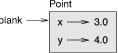
\includegraphics[scale=0.8]{../source/figs/point.pdf}}
\caption{Object diagram.}
\label{fig.point}
\end{figure}

The variable {\tt blank} refers to a Point object, which
contains two attributes.  Each attribute refers to a
floating-point number.

You can read the value of an attribute using the same syntax:

\begin{verbatim}
>>> blank.y
4.0
>>> x = blank.x
>>> x
3.0
\end{verbatim}
%
The expression {\tt blank.x} means, ``Go to the object {\tt blank}
refers to and get the value of {\tt x}.''  In the example, we assign that
value to a variable named {\tt x}.  There is no conflict between
the variable {\tt x} and the attribute {\tt x}.

You can use dot notation as part of any expression.  For example:

\begin{verbatim}
>>> '(%g, %g)' % (blank.x, blank.y)
'(3.0, 4.0)'
>>> distance = math.sqrt(blank.x**2 + blank.y**2)
>>> distance
5.0
\end{verbatim}
%
You can pass an instance as an argument in the usual way.
For example:
\index{instance!as argument}

\begin{verbatim}
def print_point(p):
    print('(%g, %g)' % (p.x, p.y))
\end{verbatim}
%
\verb"print_point" takes a point as an argument and displays it in
mathematical notation.  To invoke it, you can pass {\tt blank} as
an argument:

\begin{verbatim}
>>> print_point(blank)
(3.0, 4.0)
\end{verbatim}
%
Inside the function, {\tt p} is an alias for {\tt blank}, so if
the function modifies {\tt p}, {\tt blank} changes.
\index{aliasing}

As an exercise, write a function called \verb"distance_between_points"
that takes two Points as arguments and returns the distance between
them.


\section{Rectangles}
\label{rectangles}

Sometimes it is obvious what the attributes of an object should be,
but other times you have to make decisions.  For example, imagine you
are designing a class to represent rectangles.  What attributes would
you use to specify the location and size of a rectangle?  You can
ignore angle; to keep things simple, assume that the rectangle is
either vertical or horizontal.
\index{representation}

There are at least two possibilities:

\begin{itemize}

\item You could specify one corner of the rectangle
(or the center), the width, and the height.

\item You could specify two opposing corners.

\end{itemize}

At this point it is hard to say whether either is better than
the other, so we'll implement the first one, just as an example.
\index{Rectangle class}
\index{class!Rectangle}

Here is the class definition:

\begin{verbatim}
class Rectangle:
    """Represents a rectangle.

    attributes: width, height, corner.
    """
\end{verbatim}
%
The docstring lists the attributes:  {\tt width} and
{\tt height} are numbers; {\tt corner} is a Point object that
specifies the lower-left corner.

To represent a rectangle, you have to instantiate a Rectangle
object and assign values to the attributes:

\begin{verbatim}
box = Rectangle()
box.width = 100.0
box.height = 200.0
box.corner = Point()
box.corner.x = 0.0
box.corner.y = 0.0
\end{verbatim}
%
The expression {\tt box.corner.x} means,
``Go to the object {\tt box} refers to and select the attribute named
{\tt corner}; then go to that object and select the attribute named
{\tt x}.''

\begin{figure}
\centerline
{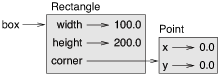
\includegraphics[scale=0.8]{../source/figs/rectangle.pdf}}
\caption{Object diagram.}
\label{fig.rectangle}
\end{figure}


Figure~\ref{fig.rectangle} shows the state of this object.
An object that is an attribute of another object is {\bf embedded}.
\index{state diagram}
\index{diagram!state}
\index{object diagram}
\index{diagram!object}
\index{embedded object}
\index{object!embedded}


\section{Instances as return values}
\index{instance!as return value}
\index{return value}

Functions can return instances.  For example, \verb"find_center"
takes a {\tt Rectangle} as an argument and returns a {\tt Point}
that contains the coordinates of the center of the {\tt Rectangle}:

\begin{verbatim}
def find_center(rect):
    p = Point()
    p.x = rect.corner.x + rect.width/2
    p.y = rect.corner.y + rect.height/2
    return p
\end{verbatim}
%
Here is an example that passes {\tt box} as an argument and assigns
the resulting Point to {\tt center}:

\begin{verbatim}
>>> center = find_center(box)
>>> print_point(center)
(50, 100)
\end{verbatim}
%

\section{Objects are mutable}
\index{object!mutable}
\index{mutability}

You can change the state of an object by making an assignment to one of
its attributes.  For example, to change the size of a rectangle
without changing its position, you can modify the values of {\tt
width} and {\tt height}:

\begin{verbatim}
box.width = box.width + 50
box.height = box.height + 100
\end{verbatim}
%
You can also write functions that modify objects.  For example,
\verb"grow_rectangle" takes a Rectangle object and two numbers,
{\tt dwidth} and {\tt dheight}, and adds the numbers to the
width and height of the rectangle:

\begin{verbatim}
def grow_rectangle(rect, dwidth, dheight):
    rect.width += dwidth
    rect.height += dheight
\end{verbatim}
%
Here is an example that demonstrates the effect:

\begin{verbatim}
>>> box.width, box.height
(150.0, 300.0)
>>> grow_rectangle(box, 50, 100)
>>> box.width, box.height
(200.0, 400.0)
\end{verbatim}
%
Inside the function, {\tt rect} is an
alias for {\tt box}, so when the function modifies {\tt rect},
{\tt box} changes.

As an exercise, write a function named \verb"move_rectangle" that takes
a Rectangle and two numbers named {\tt dx} and {\tt dy}.  It
should change the location of the rectangle by adding {\tt dx}
to the {\tt x} coordinate of {\tt corner} and adding {\tt dy}
to the {\tt y} coordinate of {\tt corner}.


\section{Copying}
\label{copying}
\index{aliasing}

Aliasing can make a program difficult to read because changes
in one place might have unexpected effects in another place.
It is hard to keep track of all the variables that might refer
to a given object.
\index{copying objects}
\index{object!copying}
\index{copy module}
\index{module!copy}

Copying an object is often an alternative to aliasing.
The {\tt copy} module contains a function called {\tt copy} that
can duplicate any object:

\begin{verbatim}
>>> p1 = Point()
>>> p1.x = 3.0
>>> p1.y = 4.0

>>> import copy
>>> p2 = copy.copy(p1)
\end{verbatim}
%
{\tt p1} and {\tt p2} contain the same data, but they are
not the same Point.

\begin{verbatim}
>>> print_point(p1)
(3, 4)
>>> print_point(p2)
(3, 4)
>>> p1 is p2
False
>>> p1 == p2
False
\end{verbatim}
%
The {\tt is} operator indicates that {\tt p1} and {\tt p2} are not the
same object, which is what we expected.  But you might have expected
{\tt ==} to yield {\tt True} because these points contain the same
data.  In that case, you will be disappointed to learn that for
instances, the default behavior of the {\tt ==} operator is the same
as the {\tt is} operator; it checks object identity, not object
equivalence.  That's because for programmer-defined types, Python doesn't
know what should be considered equivalent.  At least, not yet.
\index{is operator}
\index{operator!is}
\index{identity}
\index{equivalence}

If you use {\tt copy.copy} to duplicate a Rectangle, you will find
that it copies the Rectangle object but not the embedded Point.
\index{embedded object!copying}

\begin{verbatim}
>>> box2 = copy.copy(box)
>>> box2 is box
False
>>> box2.corner is box.corner
True
\end{verbatim}

\begin{figure}
\centerline
{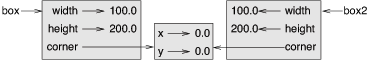
\includegraphics[scale=0.8]{../source/figs/rectangle2.pdf}}
\caption{Object diagram.}
\label{fig.rectangle2}
\end{figure}

Figure~\ref{fig.rectangle2} shows what the object diagram looks like.
\index{state diagram}
\index{diagram!state}
\index{object diagram}
\index{diagram!object}
This operation is called a {\bf shallow copy} because it copies the
object and any references it contains, but not the embedded objects.
\index{shallow copy}
\index{copy!shallow}

For most applications, this is not what you want.  In this example,
invoking \verb"grow_rectangle" on one of the Rectangles would not
affect the other, but invoking \verb"move_rectangle" on either would
affect both!  This behavior is confusing and error-prone.
\index{deep copy}
\index{copy!deep}

Fortunately, the {\tt copy} module provides a method named {\tt
deepcopy} that copies not only the object but also
the objects it refers to, and the objects {\em they} refer to,
and so on.
You will not be surprised to learn that this operation is
called a {\bf deep copy}.
\index{deepcopy function}
\index{function!deepcopy}

\begin{verbatim}
>>> box3 = copy.deepcopy(box)
>>> box3 is box
False
>>> box3.corner is box.corner
False
\end{verbatim}
%
{\tt box3} and {\tt box} are completely separate objects.

As an exercise, write a version of \verb"move_rectangle" that creates and
returns a new Rectangle instead of modifying the old one.


\section{Debugging}
\label{hasattr}
\index{debugging}

When you start working with objects, you are likely to encounter
some new exceptions.  If you try to access an attribute
that doesn't exist, you get an {\tt AttributeError}:
\index{exception!AttributeError}
\index{AttributeError}

\begin{verbatim}
>>> p = Point()
>>> p.x = 3
>>> p.y = 4
>>> p.z
AttributeError: Point instance has no attribute 'z'
\end{verbatim}
%
If you are not sure what type an object is, you can ask:
\index{type function}
\index{function!type}

\begin{verbatim}
>>> type(p)
<class '__main__.Point'>
\end{verbatim}
%
You can also use {\tt isinstance} to check whether an object
is an instance of a class:
\index{isinstance function}
\index{function!isinstance}

\begin{verbatim}
>>> isinstance(p, Point)
True
\end{verbatim}
%
If you are not sure whether an object has a particular attribute,
you can use the built-in function {\tt hasattr}:
\index{hasattr function}
\index{function!hasattr}

\begin{verbatim}
>>> hasattr(p, 'x')
True
>>> hasattr(p, 'z')
False
\end{verbatim}
%
The first argument can be any object; the second argument is a {\em
string} that contains the name of the attribute.
\index{attribute}

You can also use a {\tt try} statement to see if the object has the
attributes you need:
\index{try statement}
\index{statement!try}

\begin{verbatim}
try:
    x = p.x
except AttributeError:
    x = 0
\end{verbatim}

This approach can make it easier to write functions that work with
different types; more on that topic is
coming up in Section~\ref{polymorphism}.


\section{Glossary}

\begin{description}

\item[class:] A programmer-defined type.  A class definition creates a new
class object.
\index{class}
\index{programmer-defined type}
\index{type!programmer-defined}

\item[class object:] An object that contains information about a
programmer-defined type.  The class object can be used to create instances
of the type.
\index{class object}
\index{object!class}

\item[instance:] An object that belongs to a class.
\index{instance}

\item[instantiate:] To create a new object.
\index{instantiate}

\item[attribute:] One of the named values associated with an object.
\index{attribute!instance}
\index{instance attribute}

\item[embedded object:] An object that is stored as an attribute
of another object.
\index{embedded object}
\index{object!embedded}

\item[shallow copy:] To copy the contents of an object, including
any references to embedded objects;
implemented by the {\tt copy} function in the {\tt copy} module.
\index{shallow copy}

\item[deep copy:] To copy the contents of an object as well as any
embedded objects, and any objects embedded in them, and so on;
implemented by the {\tt deepcopy} function in the {\tt copy} module.
\index{deep copy}

\item[object diagram:] A diagram that shows objects, their
attributes, and the values of the attributes.
\index{object diagram}
\index{diagram!object}

\end{description}


\section{Exercises}

\begin{exercise}

Write a definition for a class named {\tt Circle} with attributes
{\tt center} and {\tt radius}, where {\tt center} is a Point object
and radius is a number.

Instantiate a Circle object that represents a circle with its center
at $(150, 100)$ and radius 75.

Write a function named \verb"point_in_circle" that takes a Circle and
a Point and returns True if the Point lies in or on the boundary of
the circle.

Write a function named \verb"rect_in_circle" that takes a Circle and a
Rectangle and returns True if the Rectangle lies entirely in or on the boundary
of the circle.

Write a function named \verb"rect_circle_overlap" that takes a Circle
and a Rectangle and returns True if any of the corners of the Rectangle fall
inside the circle.  Or as a more challenging version, return True if
any part of the Rectangle falls inside the circle.

Solution: \url{http://thinkpython2.com/code/Circle.py}.

\end{exercise}


\begin{exercise}

Write a function called \verb"draw_rect" that takes a Turtle object
and a Rectangle and uses the Turtle to draw the Rectangle.  See
Chapter~\ref{turtlechap} for examples using Turtle objects.

Write a function called \verb"draw_circle" that takes a Turtle and
a Circle and draws the Circle.

Solution: \url{http://thinkpython2.com/code/draw.py}.

\end{exercise}



\chapter{Classes and functions}
\label{time}

Now that we know how to create new types, the next
step is to write functions that take programmer-defined objects
as parameters and return them as results.  In this chapter I
also present ``functional programming style'' and two new
program development plans.

Code examples from this chapter are available from
\url{http://thinkpython2.com/code/Time1.py}.
Solutions to the exercises are at
\url{http://thinkpython2.com/code/Time1_soln.py}.


\section{Time}
\label{isafter}

As another example of a programmer-defined type, we'll define a class
called {\tt Time} that records the time of day.  The class definition
looks like this: \index{programmer-defined type}
\index{type!programmer-defined} \index{Time class} \index{class!Time}

\begin{verbatim}
class Time:
    """Represents the time of day.

    attributes: hour, minute, second
    """
\end{verbatim}
%
We can create a new {\tt Time} object and assign
attributes for hours, minutes, and seconds:

\begin{verbatim}
time = Time()
time.hour = 11
time.minute = 59
time.second = 30
\end{verbatim}
%
The state diagram for the {\tt Time} object looks like Figure~\ref{fig.time}.
\index{state diagram}
\index{diagram!state}
\index{object diagram}
\index{diagram!object}

As an exercise, write a function called \verb"print_time" that takes a
Time object and prints it in the form {\tt hour:minute:second}.
Hint: the format sequence \verb"'%.2d'" prints an integer using
at least two digits, including a leading zero if necessary.

Write a boolean function called \verb"is_after" that
takes two Time objects, {\tt t1} and {\tt t2}, and
returns {\tt True} if {\tt t1} follows {\tt t2} chronologically and
{\tt False} otherwise.  Challenge: don't use an {\tt if} statement.

\begin{figure}
\centerline
{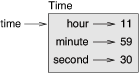
\includegraphics[scale=0.8]{../source/figs/time.pdf}}
\caption{Object diagram.}
\label{fig.time}
\end{figure}


\section{Pure functions}
\index{prototype and patch}
\index{development plan!prototype and patch}

In the next few sections, we'll write two functions that add time
values.  They demonstrate two kinds of functions: pure functions and
modifiers.  They also demonstrate a development plan I'll call {\bf
  prototype and patch}, which is a way of tackling a complex problem
by starting with a simple prototype and incrementally dealing with the
complications.

Here is a simple prototype of \verb"add_time":

\begin{verbatim}
def add_time(t1, t2):
    sum = Time()
    sum.hour = t1.hour + t2.hour
    sum.minute = t1.minute + t2.minute
    sum.second = t1.second + t2.second
    return sum
\end{verbatim}
%
The function creates a new {\tt Time} object, initializes its
attributes, and returns a reference to the new object.  This is called
a {\bf pure function} because it does not modify any of the objects
passed to it as arguments and it has no effect,
like displaying a value or getting user input,
other than returning a value.
\index{pure function}
\index{function type!pure}

To test this function, I'll create two Time objects: {\tt start}
contains the start time of a movie, like {\em Monty Python and the
Holy Grail}, and {\tt duration} contains the run time of the movie,
which is one hour 35 minutes.
\index{Monty Python and the Holy Grail}

\verb"add_time" figures out when the movie will be done.

\begin{verbatim}
>>> start = Time()
>>> start.hour = 9
>>> start.minute = 45
>>> start.second =  0

>>> duration = Time()
>>> duration.hour = 1
>>> duration.minute = 35
>>> duration.second = 0

>>> done = add_time(start, duration)
>>> print_time(done)
10:80:00
\end{verbatim}
%
The result, {\tt 10:80:00} might not be what you were hoping
for.  The problem is that this function does not deal with cases where the
number of seconds or minutes adds up to more than sixty.  When that
happens, we have to ``carry'' the extra seconds into the minute column
or the extra minutes into the hour column.
\index{carrying, addition with}

Here's an improved version:

\begin{verbatim}
def add_time(t1, t2):
    sum = Time()
    sum.hour = t1.hour + t2.hour
    sum.minute = t1.minute + t2.minute
    sum.second = t1.second + t2.second

    if sum.second >= 60:
        sum.second -= 60
        sum.minute += 1

    if sum.minute >= 60:
        sum.minute -= 60
        sum.hour += 1

    return sum
\end{verbatim}
%
Although this function is correct, it is starting to get big.
We will see a shorter alternative later.


\section{Modifiers}
\label{increment}
\index{modifier}
\index{function type!modifier}

Sometimes it is useful for a function to modify the objects it gets as
parameters.  In that case, the changes are visible to the caller.
Functions that work this way are called {\bf modifiers}.
\index{increment}

{\tt increment}, which adds a given number of seconds to a {\tt Time}
object, can be written naturally as a
modifier.  Here is a rough draft:

\begin{verbatim}
def increment(time, seconds):
    time.second += seconds

    if time.second >= 60:
        time.second -= 60
        time.minute += 1

    if time.minute >= 60:
        time.minute -= 60
        time.hour += 1
\end{verbatim}
%
The first line performs the basic operation; the remainder deals
with the special cases we saw before.
\index{special case}

Is this function correct?  What happens if {\tt seconds}
is much greater than sixty?

In that case, it is not enough to carry once; we have to keep doing it
until {\tt time.second} is less than sixty.  One solution is to
replace the {\tt if} statements with {\tt while} statements.  That
would make the function correct, but not very efficient.  As an
exercise, write a correct version of {\tt increment} that doesn't
contain any loops.

Anything that can be done with modifiers can also be done with pure
functions.  In fact, some programming languages only allow pure
functions.  There is some evidence that programs that use pure
functions are faster to develop and less error-prone than programs
that use modifiers.  But modifiers are convenient at times,
and functional programs tend to be less efficient.

In general, I recommend that you write pure functions whenever it is
reasonable and resort to modifiers only if there is a compelling
advantage.  This approach might be called a {\bf functional
programming style}.
\index{functional programming style}

As an exercise, write a ``pure'' version of {\tt increment} that
creates and returns a new Time object rather than modifying the
parameter.


\section{Prototyping versus planning}
\label{prototype}
\index{prototype and patch}
\index{development plan!prototype and patch}
\index{planned development}
\index{development plan!designed}

The development plan I am demonstrating is called ``prototype and
patch''.  For each function, I wrote a prototype that performed the
basic calculation and then tested it, patching errors along the
way.

This approach can be effective, especially if you don't yet have a
deep understanding of the problem.  But incremental corrections can
generate code that is unnecessarily complicated---since it deals with
many special cases---and unreliable---since it is hard to know if you
have found all the errors.

An alternative is {\bf designed development}, in which high-level
insight into the problem can make the programming much easier.  In
this case, the insight is that a Time object is really a three-digit
number in base 60 (see \url{http://en.wikipedia.org/wiki/Sexagesimal}.)!  The
{\tt second} attribute is the ``ones column'', the {\tt minute}
attribute is the ``sixties column'', and the {\tt hour} attribute is
the ``thirty-six hundreds column''.
\index{sexagesimal}

When we wrote \verb"add_time" and {\tt increment}, we were effectively
doing addition in base 60, which is why we had to carry from one
column to the next.
\index{carrying, addition with}

This observation suggests another approach to the whole problem---we
can convert Time objects to integers and take advantage of the fact
that the computer knows how to do integer arithmetic.

Here is a function that converts Times to integers:

\begin{verbatim}
def time_to_int(time):
    minutes = time.hour * 60 + time.minute
    seconds = minutes * 60 + time.second
    return seconds
\end{verbatim}
%
And here is a function that converts an integer to a Time
(recall that {\tt divmod} divides the first argument by the second
and returns the quotient and remainder as a tuple).
\index{divmod}

\begin{verbatim}
def int_to_time(seconds):
    time = Time()
    minutes, time.second = divmod(seconds, 60)
    time.hour, time.minute = divmod(minutes, 60)
    return time
\end{verbatim}
%
You might have to think a bit, and run some tests, to convince
yourself that these functions are correct.  One way to test them is to
check that \verb"time_to_int(int_to_time(x)) == x" for many values of
{\tt x}.  This is an example of a consistency check.
\index{consistency check}

Once you are convinced they are correct, you can use them to
rewrite \verb"add_time":

\begin{verbatim}
def add_time(t1, t2):
    seconds = time_to_int(t1) + time_to_int(t2)
    return int_to_time(seconds)
\end{verbatim}
%
This version is shorter than the original, and easier to verify.  As
an exercise, rewrite {\tt increment} using \verb"time_to_int" and
\verb"int_to_time".

In some ways, converting from base 60 to base 10 and back is harder
than just dealing with times.  Base conversion is more abstract; our
intuition for dealing with time values is better.

But if we have the insight to treat times as base 60 numbers and make
the investment of writing the conversion functions (\verb"time_to_int"
and \verb"int_to_time"), we get a program that is shorter, easier to
read and debug, and more reliable.

It is also easier to add features later.  For example, imagine
subtracting two Times to find the duration between them.  The
naive approach would be to implement subtraction with borrowing.
Using the conversion functions would be easier and more likely to be
correct.
\index{subtraction with borrowing}
\index{borrowing, subtraction with}
\index{generalization}

Ironically, sometimes making a problem harder (or more general) makes it
easier (because there are fewer special cases and fewer opportunities
for error).


\section{Debugging}
\index{debugging}

A Time object is well-formed if the values of {\tt minute} and {\tt
second} are between 0 and 60 (including 0 but not 60) and if
{\tt hour} is positive.  {\tt hour} and {\tt minute} should be
integral values, but we might allow {\tt second} to have a
fraction part.
\index{invariant}

Requirements like these are called {\bf invariants} because
they should always be true.  To put it a different way, if they
are not true, something has gone wrong.

Writing code to check invariants can help detect errors
and find their causes.  For example, you might have a function
like \verb"valid_time" that takes a Time object and returns
{\tt False} if it violates an invariant:

\begin{verbatim}
def valid_time(time):
    if time.hour < 0 or time.minute < 0 or time.second < 0:
        return False
    if time.minute >= 60 or time.second >= 60:
        return False
    return True
\end{verbatim}
%
At the beginning of each function you could check the
arguments to make sure they are valid:
\index{raise statement}
\index{statement!raise}

\begin{verbatim}
def add_time(t1, t2):
    if not valid_time(t1) or not valid_time(t2):
        raise ValueError('invalid Time object in add_time')
    seconds = time_to_int(t1) + time_to_int(t2)
    return int_to_time(seconds)
\end{verbatim}
%
Or you could use an {\bf assert statement}, which checks a given invariant
and raises an exception if it fails:
\index{assert statement}
\index{statement!assert}

\begin{verbatim}
def add_time(t1, t2):
    assert valid_time(t1) and valid_time(t2)
    seconds = time_to_int(t1) + time_to_int(t2)
    return int_to_time(seconds)
\end{verbatim}
%
{\tt assert} statements are useful because they distinguish
code that deals with normal conditions from code
that checks for errors.


\section{Glossary}

\begin{description}

\item[prototype and patch:] A development plan that involves
writing a rough draft of a program, testing, and correcting errors as
they are found.
\index{prototype and patch}

\item[designed development:] A development plan that involves
high-level insight into the problem and more planning than incremental
development or prototype development.
\index{designed development}

\item[pure function:] A function that does not modify any of the objects it
receives as arguments.  Most pure functions are fruitful.
\index{pure function}

\item[modifier:] A function that changes one or more of the objects it
  receives as arguments.  Most modifiers are void; that is, they
  return {\tt None}.  \index{modifier}

\item[functional programming style:] A style of program design in which the
majority of functions are pure.
\index{functional programming style}

\item[invariant:] A condition that should always be true during the
execution of a program.
\index{invariant}

\item[assert statement:] A statement that check a condition and raises
an exception if it fails.
\index{assert statement}
\index{statement!assert}

\end{description}


\section{Exercises}

Code examples from this chapter are available from
\url{http://thinkpython2.com/code/Time1.py}; solutions to the
exercises are available from \url{http://thinkpython2.com/code/Time1_soln.py}.

\begin{exercise}

Write a function called \verb"mul_time" that takes a Time object
and a number and returns a new Time object that contains
the product of the original Time and the number.

Then use \verb"mul_time" to write a function that takes a Time
object that represents the finishing time in a race, and a number
that represents the distance, and returns a Time object that represents
the average pace (time per mile).
\index{running pace}

\end{exercise}


\begin{exercise}
\index{datetime module}
\index{module!datetime}

The {\tt datetime} module provides {\tt time} objects
that are similar to the Time objects in this chapter, but
they provide a rich set of methods and operators.  Read the
documentation at \url{http://docs.python.org/3/library/datetime.html}.

\begin{enumerate}

\item Use the {\tt datetime} module to write a program that gets the
  current date and prints the day of the week.

\item Write a program that takes a birthday as input and prints the
  user's age and the number of days, hours, minutes and seconds until
  their next birthday.
\index{birthday}

\item For two people born on different days, there is a day when one
  is twice as old as the other.  That's their Double Day.  Write a
  program that takes two birthdays and computes their Double Day.

\item For a little more challenge, write the more general version that
  computes the day when one person is $n$ times older than the other.
\index{Double Day}

\end{enumerate}

Solution: \url{http://thinkpython2.com/code/double.py}

\end{exercise}


\chapter{Classes and methods}

Although we are using some of Python's object-oriented features,
the programs from the last two chapters are not really
object-oriented because they don't represent the relationships
between programmer-defined types and the functions that operate
on them.  The next step is to transform those functions into
methods that make the relationships explicit.

Code examples from this chapter are available from
\url{http://thinkpython2.com/code/Time2.py}, and solutions
to the exercises are in \url{http://thinkpython2.com/code/Point2_soln.py}.


\section{Object-oriented features}
\index{object-oriented programming}

Python is an {\bf object-oriented programming language}, which means
that it provides features that support object-oriented
programming, which has these defining characteristics:

\begin{itemize}

\item Programs include class and method definitions.

\item Most of the computation is expressed in terms of operations on
  objects.

\item Objects often represent things
in the real world, and methods often
correspond to the ways things in the real world interact.

\end{itemize}

For example, the {\tt Time} class defined in Chapter~\ref{time}
corresponds to the way people record the time of day, and the
functions we defined correspond to the kinds of things people do with
times.  Similarly, the {\tt Point} and {\tt Rectangle} classes
in Chapter~\ref{clobjects}
correspond to the mathematical concepts of a point and a rectangle.

So far, we have not taken advantage of the features Python provides to
support object-oriented programming.  These
features are not strictly necessary; most of them provide
alternative syntax for things we have already done.  But in many cases,
the alternative is more concise and more accurately conveys the
structure of the program.

For example, in {\tt Time1.py} there is no obvious
connection between the class definition and the function definitions
that follow.  With some examination, it is apparent that every function
takes at least one {\tt Time} object as an argument.
\index{method}
\index{function}

This observation is the motivation for {\bf methods}; a method is
a function that is associated with a particular class.
We have seen methods for strings, lists, dictionaries and tuples.
In this chapter, we will define methods for programmer-defined types.
\index{syntax}
\index{semantics}
\index{programmer-defined type}
\index{type!programmer-defined}

Methods are semantically the same as functions, but there are
two syntactic differences:

\begin{itemize}

\item Methods are defined inside a class definition in order
to make the relationship between the class and the method explicit.

\item The syntax for invoking a method is different from the
syntax for calling a function.

\end{itemize}

In the next few sections, we will take the functions from the previous
two chapters and transform them into methods.  This transformation is
purely mechanical; you can do it by following a sequence of
steps.  If you are comfortable converting from one form to another,
you will be able to choose the best form for whatever you are doing.


\section{Printing objects}
\index{object!printing}

In Chapter~\ref{time}, we defined a class named
{\tt Time} and in Section~\ref{isafter}, you
wrote a function named \verb"print_time":

\begin{verbatim}
class Time:
    """Represents the time of day."""

def print_time(time):
    print('%.2d:%.2d:%.2d' % (time.hour, time.minute, time.second))
\end{verbatim}
%
To call this function, you have to pass a {\tt Time} object as an
argument:

\begin{verbatim}
>>> start = Time()
>>> start.hour = 9
>>> start.minute = 45
>>> start.second = 00
>>> print_time(start)
09:45:00
\end{verbatim}
%
To make \verb"print_time" a method, all we have to do is
move the function definition inside the class definition.  Notice
the change in indentation.
\index{indentation}

\begin{verbatim}
class Time:
    def print_time(time):
        print('%.2d:%.2d:%.2d' % (time.hour, time.minute, time.second))
\end{verbatim}
%
Now there are two ways to call \verb"print_time".  The first
(and less common) way is to use function syntax:
\index{function syntax}
\index{dot notation}

\begin{verbatim}
>>> Time.print_time(start)
09:45:00
\end{verbatim}
%
In this use of dot notation, {\tt Time} is the name of the class,
and \verb"print_time" is the name of the method.  {\tt start} is
passed as a parameter.

The second (and more concise) way is to use method syntax:
\index{method syntax}

\begin{verbatim}
>>> start.print_time()
09:45:00
\end{verbatim}
%
In this use of dot notation, \verb"print_time" is the name of the
method (again), and {\tt start} is the object the method is
invoked on, which is called the {\bf subject}.  Just as the
subject of a sentence is what the sentence is about, the subject
of a method invocation is what the method is about.
\index{subject}

Inside the method, the subject is assigned to the first
parameter, so in this case {\tt start} is assigned
to {\tt time}.
\index{self (parameter name)}
\index{parameter!self}

By convention, the first parameter of a method is
called {\tt self}, so it would be more common to write
\verb"print_time" like this:

\begin{verbatim}
class Time:
    def print_time(self):
        print('%.2d:%.2d:%.2d' % (self.hour, self.minute, self.second))
\end{verbatim}
%
The reason for this convention is an implicit metaphor:
\index{metaphor, method invocation}

\begin{itemize}

\item The syntax for a function call, \verb"print_time(start)",
  suggests that the function is the active agent.  It says something
  like, ``Hey \verb"print_time"!  Here's an object for you to print.''

\item In object-oriented programming, the objects are the active
  agents.  A method invocation like \verb"start.print_time()" says
  ``Hey {\tt start}!  Please print yourself.''

\end{itemize}

This change in perspective might be more polite, but it is not obvious
that it is useful.  In the examples we have seen so far, it may not
be.  But sometimes shifting responsibility from the functions onto the
objects makes it possible to write more versatile functions (or
methods), and makes it easier to maintain and reuse code.

As an exercise, rewrite \verb"time_to_int" (from
Section~\ref{prototype}) as a method.  You might be tempted to
rewrite \verb"int_to_time" as a method, too, but that doesn't
really make sense because there would be no object to invoke
it on.


\section{Another example}
\index{increment}

Here's a version of {\tt increment} (from Section~\ref{increment})
rewritten as a method:

\begin{verbatim}
# inside class Time:

    def increment(self, seconds):
        seconds += self.time_to_int()
        return int_to_time(seconds)
\end{verbatim}
%
This version assumes that \verb"time_to_int" is written
as a method.  Also, note that
it is a pure function, not a modifier.

Here's how you would invoke {\tt increment}:

\begin{verbatim}
>>> start.print_time()
09:45:00
>>> end = start.increment(1337)
>>> end.print_time()
10:07:17
\end{verbatim}
%
The subject, {\tt start}, gets assigned to the first parameter,
{\tt self}.  The argument, {\tt 1337}, gets assigned to the
second parameter, {\tt seconds}.

This mechanism can be confusing, especially if you make an error.
For example, if you invoke {\tt increment} with two arguments, you
get:
\index{exception!TypeError}
\index{TypeError}

\begin{verbatim}
>>> end = start.increment(1337, 460)
TypeError: increment() takes 2 positional arguments but 3 were given
\end{verbatim}
%
The error message is initially confusing, because there are
only two arguments in parentheses.  But the subject is also
considered an argument, so all together that's three.

By the way, a {\bf positional argument} is an argument that
doesn't have a parameter name; that is, it is not a keyword
argument.  In this function call:
\index{positional argument}
\index{argument!positional}

\begin{verbatim}
sketch(parrot, cage, dead=True)
\end{verbatim}

{\tt parrot} and {\tt cage} are positional, and {\tt dead} is
a keyword argument.


\section{A more complicated example}

Rewriting \verb"is_after" (from Section~\ref{isafter}) is slightly
more complicated because it takes two Time objects as parameters.  In
this case it is conventional to name the first parameter {\tt self}
and the second parameter {\tt other}: \index{other (parameter name)}
\index{parameter!other}

\begin{verbatim}
# inside class Time:

    def is_after(self, other):
        return self.time_to_int() > other.time_to_int()
\end{verbatim}
%
To use this method, you have to invoke it on one object and pass
the other as an argument:

\begin{verbatim}
>>> end.is_after(start)
True
\end{verbatim}
%
One nice thing about this syntax is that it almost reads
like English: ``end is after start?''


\section{The init method}
\index{init method}
\index{method!init}

The init method (short for ``initialization'') is
a special method that gets invoked when an object is instantiated.
Its full name is \verb"__init__" (two underscore characters,
followed by {\tt init}, and then two more underscores).  An
init method for the {\tt Time} class might look like this:

\begin{verbatim}
# inside class Time:

    def __init__(self, hour=0, minute=0, second=0):
        self.hour = hour
        self.minute = minute
        self.second = second
\end{verbatim}
%
It is common for the parameters of \verb"__init__"
to have the same names as the attributes.  The statement

\begin{verbatim}
        self.hour = hour
\end{verbatim}
%
stores the value of the parameter {\tt hour} as an attribute
of {\tt self}.
\index{optional parameter}
\index{parameter!optional}
\index{default value}
\index{override}

The parameters are optional, so if you call {\tt Time} with
no arguments, you get the default values.

\begin{verbatim}
>>> time = Time()
>>> time.print_time()
00:00:00
\end{verbatim}
%
If you provide one argument, it overrides {\tt hour}:

\begin{verbatim}
>>> time = Time (9)
>>> time.print_time()
09:00:00
\end{verbatim}
%
If you provide two arguments, they override {\tt hour} and
{\tt minute}.

\begin{verbatim}
>>> time = Time(9, 45)
>>> time.print_time()
09:45:00
\end{verbatim}
%
And if you provide three arguments, they override all three
default values.

As an exercise, write an init method for the {\tt Point} class that takes
{\tt x} and {\tt y} as optional parameters and assigns
them to the corresponding attributes.
\index{Point class}
\index{class!Point}


\section{The {\tt \_\_str\_\_} method}
\index{str method@\_\_str\_\_ method}
\index{method!\_\_str\_\_}

\verb"__str__" is a special method, like \verb"__init__",
that is supposed to return a string representation of an object.
\index{string representation}

For example, here is a {\tt str} method for Time objects:

\begin{verbatim}
# inside class Time:

    def __str__(self):
        return '%.2d:%.2d:%.2d' % (self.hour, self.minute, self.second)
\end{verbatim}
%
When you {\tt print} an object, Python invokes the {\tt str} method:
\index{print statement}
\index{statement!print}

\begin{verbatim}
>>> time = Time(9, 45)
>>> print(time)
09:45:00
\end{verbatim}
%
When I write a new class, I almost always start by writing
\verb"__init__", which makes it easier to instantiate objects, and
\verb"__str__", which is useful for debugging.

As an exercise, write a {\tt str} method for the {\tt Point} class.
Create a Point object and print it.


\section{Operator overloading}
\label{operator.overloading}

By defining other special methods, you can specify the behavior
of operators on programmer-defined types.  For example, if you define
a method named \verb"__add__" for the {\tt Time} class, you can use the
{\tt +} operator on Time objects.
\index{programmer-defined type}
\index{type!programmer-defined}

Here is what the definition might look like:
\index{add method}
\index{method!add}

\begin{verbatim}
# inside class Time:

    def __add__(self, other):
        seconds = self.time_to_int() + other.time_to_int()
        return int_to_time(seconds)
\end{verbatim}
%
And here is how you could use it:

\begin{verbatim}
>>> start = Time(9, 45)
>>> duration = Time(1, 35)
>>> print(start + duration)
11:20:00
\end{verbatim}
%
When you apply the {\tt +} operator to Time objects, Python invokes
\verb"__add__".  When you print the result, Python invokes
\verb"__str__".  So there is a lot happening behind the scenes!
\index{operator overloading}

Changing the behavior of an operator so that it works with
programmer-defined types is called {\bf operator overloading}.  For every
operator in Python there is a corresponding special method, like
\verb"__add__".  For more details, see
\url{http://docs.python.org/3/reference/datamodel.html#specialnames}.

As an exercise, write an {\tt add} method for the Point class.


\section{Type-based dispatch}

In the previous section we added two Time objects, but you
also might want to add an integer to a Time object.  The
following is a version of \verb"__add__"
that checks the type of {\tt other} and invokes either
\verb"add_time" or {\tt increment}:

\begin{verbatim}
# inside class Time:

    def __add__(self, other):
        if isinstance(other, Time):
            return self.add_time(other)
        else:
            return self.increment(other)

    def add_time(self, other):
        seconds = self.time_to_int() + other.time_to_int()
        return int_to_time(seconds)

    def increment(self, seconds):
        seconds += self.time_to_int()
        return int_to_time(seconds)
\end{verbatim}
%
The built-in function {\tt isinstance} takes a value and a
class object, and returns {\tt True} if the value is an instance
of the class.
\index{isinstance function}
\index{function!isinstance}

If {\tt other} is a Time object, \verb"__add__" invokes
\verb"add_time".  Otherwise it assumes that the parameter
is a number and invokes {\tt increment}.  This operation is
called a {\bf type-based dispatch} because it dispatches the
computation to different methods based on the type of the
arguments.
\index{type-based dispatch}
\index{dispatch, type-based}

Here are examples that use the {\tt +} operator with different
types:

\begin{verbatim}
>>> start = Time(9, 45)
>>> duration = Time(1, 35)
>>> print(start + duration)
11:20:00
>>> print(start + 1337)
10:07:17
\end{verbatim}
%
Unfortunately, this implementation of addition is not commutative.
If the integer is the first operand, you get
\index{commutativity}

\begin{verbatim}
>>> print(1337 + start)
TypeError: unsupported operand type(s) for +: 'int' and 'instance'
\end{verbatim}
%
The problem is, instead of asking the Time object to add an integer,
Python is asking an integer to add a Time object, and it doesn't know
how.  But there is a clever solution for this problem: the
special method \verb"__radd__", which stands for ``right-side add''.
This method is invoked when a Time object appears on the right side of
the {\tt +} operator.  Here's the definition:
\index{radd method}
\index{method!radd}

\begin{verbatim}
# inside class Time:

    def __radd__(self, other):
        return self.__add__(other)
\end{verbatim}
%
And here's how it's used:

\begin{verbatim}
>>> print(1337 + start)
10:07:17
\end{verbatim}
%

As an exercise, write an {\tt add} method for Points that works with
either a Point object or a tuple:

\begin{itemize}

\item If the second operand is a Point, the method should return a new
Point whose $x$ coordinate is the sum of the $x$ coordinates of the
operands, and likewise for the $y$ coordinates.

\item If the second operand is a tuple, the method should add the
first element of the tuple to the $x$ coordinate and the second
element to the $y$ coordinate, and return a new Point with the result.

\end{itemize}




\section{Polymorphism}
\label{polymorphism}

Type-based dispatch is useful when it is necessary, but (fortunately)
it is not always necessary.  Often you can avoid it by writing functions
that work correctly for arguments with different types.
\index{type-based dispatch}
\index{dispatch!type-based}

Many of the functions we wrote for strings also
work for other sequence types.
For example, in Section~\ref{histogram}
we used {\tt histogram} to count the number of times each letter
appears in a word.

\begin{verbatim}
def histogram(s):
    d = dict()
    for c in s:
        if c not in d:
            d[c] = 1
        else:
            d[c] = d[c]+1
    return d
\end{verbatim}
%
This function also works for lists, tuples, and even dictionaries,
as long as the elements of {\tt s} are hashable, so they can be used
as keys in {\tt d}.

\begin{verbatim}
>>> t = ['spam', 'egg', 'spam', 'spam', 'bacon', 'spam']
>>> histogram(t)
{'bacon': 1, 'egg': 1, 'spam': 4}
\end{verbatim}
%
Functions that work with several types are called {\bf polymorphic}.
Polymorphism can facilitate code reuse.  For example, the built-in
function {\tt sum}, which adds the elements of a sequence, works
as long as the elements of the sequence support addition.
\index{polymorphism}

Since Time objects provide an {\tt add} method, they work
with {\tt sum}:

\begin{verbatim}
>>> t1 = Time(7, 43)
>>> t2 = Time(7, 41)
>>> t3 = Time(7, 37)
>>> total = sum([t1, t2, t3])
>>> print(total)
23:01:00
\end{verbatim}
%
In general, if all of the operations inside a function
work with a given type, the function works with that type.

The best kind of polymorphism is the unintentional kind, where
you discover that a function you already wrote can be
applied to a type you never planned for.


\section{Debugging}
\index{debugging}

It is legal to add attributes to objects at any point in the execution
of a program, but if you have objects with the same type that don't
have the same attributes, it is easy to make mistakes.
It is considered a good idea to
initialize all of an object's attributes in the init method.
\index{init method}
\index{attribute!initializing}

If you are not sure whether an object has a particular attribute, you
can use the built-in function {\tt hasattr} (see Section~\ref{hasattr}).
\index{hasattr function}
\index{function!hasattr}
\index{dict attribute@\_\_dict\_\_ attribute}
\index{attribute!\_\_dict\_\_}

Another way to access attributes is the built-in function {\tt vars},
which takes an object and returns a dictionary that maps from
attribute names (as strings) to their values:

\begin{verbatim}
>>> p = Point(3, 4)
>>> vars(p)
{'y': 4, 'x': 3}
\end{verbatim}
%
For purposes of debugging, you might find it useful to keep this
function handy:

\begin{verbatim}
def print_attributes(obj):
    for attr in vars(obj):
        print(attr, getattr(obj, attr))
\end{verbatim}
%
\verb"print_attributes" traverses the dictionary
and prints each attribute name and its corresponding value.
\index{traversal!dictionary}
\index{dictionary!traversal}

The built-in function {\tt getattr} takes an object and an attribute
name (as a string) and returns the attribute's value.
\index{getattr function}
\index{function!getattr}


\section{Interface and implementation}

One of the goals of object-oriented design is to make software more
maintainable, which means that you can keep the program working when
other parts of the system change, and modify the program to meet new
requirements.
\index{interface}
\index{implementation}
\index{maintainable}
\index{object-oriented design}

A design principle that helps achieve that goal is to keep
interfaces separate from implementations.  For objects, that means
that the methods a class provides should not depend on how the
attributes are represented.
\index{attribute}

For example, in this chapter we developed a class that represents
a time of day.  Methods provided by this class include
\verb"time_to_int", \verb"is_after", and \verb"add_time".

We could implement those methods in several ways.  The details of the
implementation depend on how we represent time.  In this chapter, the
attributes of a {\tt Time} object are {\tt hour}, {\tt minute}, and
{\tt second}.

As an alternative, we could replace these attributes with
a single integer representing the number of seconds
since midnight.  This implementation would make some methods,
like \verb"is_after", easier to write, but it makes other methods
harder.

After you deploy a new class, you might discover a better
implementation.  If other parts of the program are using your
class, it might be time-consuming and error-prone to change the
interface.

But if you designed the interface carefully, you can
change the implementation without changing the interface, which
means that other parts of the program don't have to change.


\section{Glossary}

\begin{description}

\item[object-oriented language:] A language that provides features,
  such as programmer-defined types and methods, that facilitate
  object-oriented programming.
\index{object-oriented language}

\item[object-oriented programming:] A style of programming in which
data and the operations that manipulate it are organized into classes
and methods.
\index{object-oriented programming}

\item[method:] A function that is defined inside a class definition and
is invoked on instances of that class.
\index{method}

\item[subject:] The object a method is invoked on.
\index{subject}

\item[positional argument:]  An argument that does not include
a parameter name, so it is not a keyword argument.
\index{positional argument}
\index{argument!positional}

\item[operator overloading:] Changing the behavior of an operator like
{\tt +} so it works with a programmer-defined type.
\index{overloading}
\index{operator!overloading}

\item[type-based dispatch:] A programming pattern that checks the type
of an operand and invokes different functions for different types.
\index{type-based dispatch}

\item[polymorphic:] Pertaining to a function that can work with more
  than one type.
\index{polymorphism}

\item[information hiding:] The principle that the interface provided
by an object should not depend on its implementation, in particular
the representation of its attributes.
\index{information hiding}

\end{description}


\section{Exercises}

\begin{exercise}

Download the code from this chapter from
\url{http://thinkpython2.com/code/Time2.py}.  Change the attributes of
    {\tt Time} to be a single integer representing seconds since
    midnight.  Then modify the methods (and the function
    \verb"int_to_time") to work with the new implementation.  You
    should not have to modify the test code in {\tt main}.  When you
    are done, the output should be the same as before.  Solution:
    \url{http://thinkpython2.com/code/Time2_soln.py}.

\end{exercise}


\begin{exercise}
\label{kangaroo}
\index{default value!avoiding mutable}
\index{mutable object, as default value}
\index{worst bug}
\index{bug!worst}
\index{Kangaroo class}
\index{class!Kangaroo}

This exercise is a cautionary tale about one of the most
common, and difficult to find, errors in Python.
Write a definition for a class named {\tt Kangaroo} with the following
methods:

\begin{enumerate}

\item An \verb"__init__" method that initializes an attribute named
\verb"pouch_contents" to an empty list.

\item A method named \verb"put_in_pouch" that takes an object
of any type and adds it to \verb"pouch_contents".

\item A \verb"__str__" method that returns a string representation
of the Kangaroo object and the contents of the pouch.

\end{enumerate}
%
Test your code
by creating two {\tt Kangaroo} objects, assigning them to variables
named {\tt kanga} and {\tt roo}, and then adding {\tt roo} to the
contents of {\tt kanga}'s pouch.

Download \url{http://thinkpython2.com/code/BadKangaroo.py}.  It contains
a solution to the previous problem with one big, nasty bug.
Find and fix the bug.

If you get stuck, you can download
\url{http://thinkpython2.com/code/GoodKangaroo.py}, which explains the
problem and demonstrates a solution.
\index{aliasing}
\index{embedded object}
\index{object!embedded}

\end{exercise}



\chapter{Inheritance}

The language feature most often associated with object-oriented
programming is {\bf inheritance}.  Inheritance is the ability to
define a new class that is a modified version of an existing class.
In this chapter I demonstrate inheritance using classes that represent
playing cards, decks of cards, and poker hands.
\index{deck}
\index{card, playing}
\index{poker}

If you don't play
poker, you can read about it at
\url{http://en.wikipedia.org/wiki/Poker}, but you don't have to; I'll
tell you what you need to know for the exercises.

Code examples from
this chapter are available from
\url{http://thinkpython2.com/code/Card.py}.


\section{Card objects}

There are fifty-two cards in a deck, each of which belongs to one of
four suits and one of thirteen ranks.  The suits are Spades, Hearts,
Diamonds, and Clubs (in descending order in bridge).  The ranks are
Ace, 2, 3, 4, 5, 6, 7, 8, 9, 10, Jack, Queen, and King.  Depending on
the game that you are playing, an Ace may be higher than King
or lower than 2.
\index{rank}
\index{suit}

If we want to define a new object to represent a playing card, it is
obvious what the attributes should be: {\tt rank} and
{\tt suit}.  It is not as obvious what type the attributes
should be.  One possibility is to use strings containing words like
\verb"'Spade'" for suits and \verb"'Queen'" for ranks.  One problem with
this implementation is that it would not be easy to compare cards to
see which had a higher rank or suit.
\index{encode}
\index{encrypt}
\index{map to}
\index{representation}

An alternative is to use integers to {\bf encode} the ranks and suits.
In this context, ``encode'' means that we are going to define a mapping
between numbers and suits, or between numbers and ranks.  This
kind of encoding is not meant to be a secret (that
would be ``encryption'').

\newcommand{\mymapsto}{$\mapsto$}

For example, this table shows the suits and the corresponding integer
codes:

\begin{tabular}{l c l}
Spades & \mymapsto & 3 \\
Hearts & \mymapsto & 2 \\
Diamonds & \mymapsto & 1 \\
Clubs & \mymapsto & 0
\end{tabular}

This code makes it easy to compare cards; because higher suits map to
higher numbers, we can compare suits by comparing their codes.

The mapping for ranks is fairly obvious; each of the numerical ranks
maps to the corresponding integer, and for face cards:

\begin{tabular}{l c l}
Jack & \mymapsto & 11 \\
Queen & \mymapsto & 12 \\
King & \mymapsto & 13 \\
\end{tabular}

I am using the \mymapsto~symbol to make it clear that these mappings
are not part of the Python program.  They are part of the program
design, but they don't appear explicitly in the code.
\index{Card class}
\index{class!Card}

The class definition for {\tt Card} looks like this:

\begin{verbatim}
class Card:
    """Represents a standard playing card."""

    def __init__(self, suit=0, rank=2):
        self.suit = suit
        self.rank = rank
\end{verbatim}
%
As usual, the init method takes an optional
parameter for each attribute.  The default card is
the 2 of Clubs.
\index{init method}
\index{method!init}

To create a Card, you call {\tt Card} with the
suit and rank of the card you want.

\begin{verbatim}
queen_of_diamonds = Card(1, 12)
\end{verbatim}
%


\section{Class attributes}
\label{class.attribute}
\index{class attribute}
\index{attribute!class}

In order to print Card objects in a way that people can easily
read, we need a mapping from the integer codes to the corresponding
ranks and suits.  A natural way to
do that is with lists of strings.  We assign these lists to {\bf class
attributes}:

\begin{verbatim}
# inside class Card:

    suit_names = ['Clubs', 'Diamonds', 'Hearts', 'Spades']
    rank_names = [None, 'Ace', '2', '3', '4', '5', '6', '7',
              '8', '9', '10', 'Jack', 'Queen', 'King']

    def __str__(self):
        return '%s of %s' % (Card.rank_names[self.rank],
                             Card.suit_names[self.suit])
\end{verbatim}
%
Variables like \verb"suit_names" and \verb"rank_names", which are
defined inside a class but outside of any method, are called
class attributes because they are associated with the class object
{\tt Card}.
\index{instance attribute}
\index{attribute!instance}

This term distinguishes them from variables like {\tt suit} and {\tt
  rank}, which are called {\bf instance attributes} because they are
associated with a particular instance.
\index{dot notation}

Both kinds of attribute are accessed using dot notation.  For
example, in \verb"__str__", {\tt self} is a Card object,
and {\tt self.rank} is its rank.  Similarly, {\tt Card}
is a class object, and \verb"Card.rank_names" is a
list of strings associated with the class.

Every card has its own {\tt suit} and {\tt rank}, but there
is only one copy of \verb"suit_names" and \verb"rank_names".

Putting it all together, the expression
\verb"Card.rank_names[self.rank]" means ``use the attribute {\tt rank}
from the object {\tt self} as an index into the list \verb"rank_names"
from the class {\tt Card}, and select the appropriate string.''

The first element of \verb"rank_names" is {\tt None} because there
is no card with rank zero.  By including {\tt None} as a place-keeper,
we get a mapping with the nice property that the index 2 maps to the
string \verb"'2'", and so on.  To avoid this tweak, we could have
used a dictionary instead of a list.

With the methods we have so far, we can create and print cards:

\begin{verbatim}
>>> card1 = Card(2, 11)
>>> print(card1)
Jack of Hearts
\end{verbatim}

\begin{figure}
\centerline
{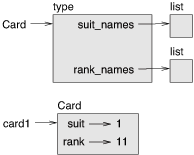
\includegraphics[scale=0.8]{../source/figs/card1.pdf}}
\caption{Object diagram.}
\label{fig.card1}
\end{figure}

Figure~\ref{fig.card1} is a diagram of the {\tt Card} class object and
one Card instance.  {\tt Card} is a class object; its type is {\tt
  type}.  {\tt card1} is an instance of {\tt Card}, so its type is
{\tt Card}.  To save space, I didn't draw the contents of
\verb"suit_names" and \verb"rank_names".  \index{state diagram}
\index{diagram!state} \index{object diagram} \index{diagram!object}


\section{Comparing cards}
\label{comparecard}
\index{operator!relational}
\index{relational operator}

For built-in types, there are relational operators
({\tt <}, {\tt >}, {\tt ==}, etc.)
that compare
values and determine when one is greater than, less than, or equal to
another.  For programmer-defined types, we can override the behavior of
the built-in operators by providing a method named
\verb"__lt__", which stands for ``less than''.
\index{programmer-defined type}
\index{type!programmer-defined}

\verb"__lt__" takes two parameters, {\tt self} and {\tt other},
and {\tt True} if {\tt self} is strictly less than {\tt other}.
\index{override}
\index{operator overloading}

The correct ordering for cards is not obvious.
For example, which
is better, the 3 of Clubs or the 2 of Diamonds?  One has a higher
rank, but the other has a higher suit.  In order to compare
cards, you have to decide whether rank or suit is more important.

The answer might depend on what game you are playing, but to keep
things simple, we'll make the arbitrary choice that suit is more
important, so all of the Spades outrank all of the Diamonds,
and so on.
\index{cmp method@\_\_cmp\_\_ method}
\index{method!\_\_cmp\_\_}

With that decided, we can write \verb"__lt__":

\begin{verbatim}
# inside class Card:

    def __lt__(self, other):
        # check the suits
        if self.suit < other.suit: return True
        if self.suit > other.suit: return False

        # suits are the same... check ranks
        return self.rank < other.rank
\end{verbatim}
%
You can write this more concisely using tuple comparison:
\index{tuple!comparison}
\index{comparison!tuple}

\begin{verbatim}
# inside class Card:

    def __lt__(self, other):
        t1 = self.suit, self.rank
        t2 = other.suit, other.rank
        return t1 < t2
\end{verbatim}
%
As an exercise, write an \verb"__lt__" method for Time objects.  You
can use tuple comparison, but you also might consider
comparing integers.


\section{Decks}
\index{list!of objects}
\index{deck, playing cards}

Now that we have Cards, the next step is to define Decks.  Since a
deck is made up of cards, it is natural for each Deck to contain a
list of cards as an attribute.
\index{init method}
\index{method!init}

The following is a class definition for {\tt Deck}.  The
init method creates the attribute {\tt cards} and generates
the standard set of fifty-two cards:
\index{composition}
\index{loop!nested}
\index{Deck class}
\index{class!Deck}

\begin{verbatim}
class Deck:

    def __init__(self):
        self.cards = []
        for suit in range(4):
            for rank in range(1, 14):
                card = Card(suit, rank)
                self.cards.append(card)
\end{verbatim}
%
The easiest way to populate the deck is with a nested loop.  The outer
loop enumerates the suits from 0 to 3.  The inner loop enumerates the
ranks from 1 to 13.  Each iteration
creates a new Card with the current suit and rank,
and appends it to {\tt self.cards}.
\index{append method}
\index{method!append}


\section{Printing the deck}
\label{printdeck}
\index{str method@\_\_str\_\_ method}
\index{method!\_\_str\_\_}

Here is a \verb"__str__" method for {\tt Deck}:

\begin{verbatim}
#inside class Deck:

    def __str__(self):
        res = []
        for card in self.cards:
            res.append(str(card))
        return '\n'.join(res)
\end{verbatim}
%
This method demonstrates an efficient way to accumulate a large
string: building a list of strings and then using the string method
{\tt join}.  The built-in function {\tt str} invokes the
\verb"__str__" method on each card and returns the string
representation.  \index{accumulator!string} \index{string!accumulator}
\index{join method} \index{method!join} \index{newline}

Since we invoke {\tt join} on a newline character, the cards
are separated by newlines.  Here's what the result looks like:

\begin{verbatim}
>>> deck = Deck()
>>> print(deck)
Ace of Clubs
2 of Clubs
3 of Clubs
...
10 of Spades
Jack of Spades
Queen of Spades
King of Spades
\end{verbatim}
%
Even though the result appears on 52 lines, it is
one long string that contains newlines.


\section{Add, remove, shuffle and sort}

To deal cards, we would like a method that
removes a card from the deck and returns it.
The list method {\tt pop} provides a convenient way to do that:
\index{pop method}
\index{method!pop}

\begin{verbatim}
#inside class Deck:

    def pop_card(self):
        return self.cards.pop()
\end{verbatim}
%
Since {\tt pop} removes the {\em last} card in the list, we are
dealing from the bottom of the deck.
\index{append method}
\index{method!append}

To add a card, we can use the list method {\tt append}:

\begin{verbatim}
#inside class Deck:

    def add_card(self, card):
        self.cards.append(card)
\end{verbatim}
%
A method like this that uses another method without doing
much work is sometimes called a {\bf veneer}.  The metaphor
comes from woodworking, where a veneer is a thin
layer of good quality wood glued to the surface of a cheaper piece of
wood to improve the appearance.
\index{veneer}

In this case \verb"add_card" is a ``thin'' method that expresses
a list operation in terms appropriate for decks.  It
improves the appearance, or interface, of the
implementation.

As another example, we can write a Deck method named {\tt shuffle}
using the function {\tt shuffle} from the {\tt random} module:
\index{random module}
\index{module!random}
\index{shuffle function}
\index{function!shuffle}

\begin{verbatim}
# inside class Deck:

    def shuffle(self):
        random.shuffle(self.cards)
\end{verbatim}
%
Don't forget to import {\tt random}.

As an exercise, write a Deck method named {\tt sort} that uses the
list method {\tt sort} to sort the cards in a {\tt Deck}.  {\tt sort}
uses the \verb"__lt__" method we defined to determine the order.
\index{sort method} \index{method!sort}



\section{Inheritance}
\index{inheritance}
\index{object-oriented programming}

Inheritance is the ability to define a new class that is a modified
version of an existing class.  As an example, let's say we want a
class to represent a ``hand'', that is, the cards held by one player.
A hand is similar to a deck: both are made up of a collection of
cards, and both require operations like adding and removing cards.

A hand is also different from a deck; there are operations we want for
hands that don't make sense for a deck.  For example, in poker we
might compare two hands to see which one wins.  In bridge, we might
compute a score for a hand in order to make a bid.

This relationship between classes---similar, but different---lends
itself to inheritance.
To define a new class that inherits from an existing class,
you put the name of the existing class in parentheses:
\index{parentheses!parent class in}
\index{parent class}
\index{class!parent}
\index{Hand class}
\index{class!Hand}

\begin{verbatim}
class Hand(Deck):
    """Represents a hand of playing cards."""
\end{verbatim}
%
This definition indicates that {\tt Hand} inherits from {\tt Deck};
that means we can use methods like \verb"pop_card" and \verb"add_card"
for Hands as well as Decks.

When a new class inherits from an existing one, the existing
one is called the {\bf parent} and the new class is
called the {\bf child}.
\index{parent class}
\index{child class}
\index{class!child}

In this example, {\tt Hand} inherits \verb"__init__" from {\tt Deck},
but it doesn't really do what we want: instead of populating the hand
with 52 new cards, the init method for Hands should initialize {\tt
  cards} with an empty list.  \index{override} \index{init method}
\index{method!init}

If we provide an init method in the {\tt Hand} class, it overrides the
one in the {\tt Deck} class:

\begin{verbatim}
# inside class Hand:

    def __init__(self, label=''):
        self.cards = []
        self.label = label
\end{verbatim}
%
When you create a Hand, Python invokes this init method, not the
one in {\tt Deck}.

\begin{verbatim}
>>> hand = Hand('new hand')
>>> hand.cards
[]
>>> hand.label
'new hand'
\end{verbatim}
%
The other methods are inherited from {\tt Deck}, so we can use
\verb"pop_card" and \verb"add_card" to deal a card:

\begin{verbatim}
>>> deck = Deck()
>>> card = deck.pop_card()
>>> hand.add_card(card)
>>> print(hand)
King of Spades
\end{verbatim}
%
A natural next step is to encapsulate this code in a method
called \verb"move_cards":
\index{encapsulation}

\begin{verbatim}
#inside class Deck:

    def move_cards(self, hand, num):
        for i in range(num):
            hand.add_card(self.pop_card())
\end{verbatim}
%
\verb"move_cards" takes two arguments, a Hand object and the number of
cards to deal.  It modifies both {\tt self} and {\tt hand}, and
returns {\tt None}.

In some games, cards are moved from one hand to another,
or from a hand back to the deck.  You can use \verb"move_cards"
for any of these operations: {\tt self} can be either a Deck
or a Hand, and {\tt hand}, despite the name, can also be a {\tt Deck}.

Inheritance is a useful feature.  Some programs that would be
repetitive without inheritance can be written more elegantly
with it.  Inheritance can facilitate code reuse, since you can
customize the behavior of parent classes without having to modify
them.  In some cases, the inheritance structure reflects the natural
structure of the problem, which makes the design easier to
understand.

On the other hand, inheritance can make programs difficult to read.
When a method is invoked, it is sometimes not clear where to find its
definition.  The relevant code may be spread across several modules.
Also, many of the things that can be done using inheritance can be
done as well or better without it.


\section{Class diagrams}
\label{class.diagram}

So far we have seen stack diagrams, which show the state of
a program, and object diagrams, which show the attributes
of an object and their values.  These diagrams represent a snapshot
in the execution of a program, so they change as the program
runs.

They are also highly detailed; for some purposes, too
detailed.  A class diagram is a more abstract representation
of the structure of a program.  Instead of showing individual
objects, it shows classes and the relationships between them.

There are several kinds of relationship between classes:

\begin{itemize}

\item Objects in one class might contain references to objects
in another class.  For example, each Rectangle contains a reference
to a Point, and each Deck contains references to many Cards.
This kind of relationship is called {\bf HAS-A}, as in, ``a Rectangle
has a Point.''

\item One class might inherit from another.  This relationship
is called {\bf IS-A}, as in, ``a Hand is a kind of a Deck.''

\item One class might depend on another in the sense that objects
in one class take objects in the second class as parameters, or
use objects in the second class as part of a computation.  This
kind of relationship is called a {\bf dependency}.

\end{itemize}
\index{IS-A relationship}
\index{HAS-A relationship}
\index{class diagram}
\index{diagram!class}

A {\bf class diagram} is a graphical representation of these
relationships.  For example, Figure~\ref{fig.class1} shows the
relationships between {\tt Card}, {\tt Deck} and {\tt Hand}.

\begin{figure}
\centerline
{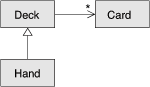
\includegraphics[scale=0.8]{../source/figs/class1.pdf}}
\caption{Class diagram.}
\label{fig.class1}
\end{figure}

The arrow with a hollow triangle head represents an IS-A
relationship; in this case it indicates that Hand inherits
from Deck.

The standard arrow head represents a HAS-A
relationship; in this case a Deck has references to Card
objects.
\index{multiplicity (in class diagram)}

The star ({\tt *}) near the arrow head is a
{\bf multiplicity}; it indicates how many Cards a Deck has.
A multiplicity can be a simple number, like {\tt 52}, a range,
like {\tt 5..7} or a star, which indicates that a Deck can
have any number of Cards.

There are no dependencies in this diagram.  They would normally
be shown with a dashed arrow.  Or if there are a lot of
dependencies, they are sometimes omitted.

A more detailed diagram might show that a Deck actually
contains a {\em list} of Cards, but built-in types
like list and dict are usually not included in class diagrams.


\section{Debugging}
\index{debugging}

Inheritance can make debugging difficult because when you invoke a
method on an object, it might be hard to figure out which method will
be invoked.
\index{inheritance}

Suppose you are writing a function that works with Hand objects.
You would like it to work with all kinds of Hands, like
PokerHands, BridgeHands, etc.  If you invoke a method like
{\tt shuffle}, you might get the one defined in {\tt Deck},
but if any of the subclasses override this method, you'll
get that version instead.  This behavior is usually a good
thing, but it can be confusing.

Any time you are unsure about the flow of execution through your
program, the simplest solution is to add print statements at the
beginning of the relevant methods.  If {\tt Deck.shuffle} prints a
message that says something like {\tt Running Deck.shuffle}, then as
the program runs it traces the flow of execution.
\index{flow of execution}

As an alternative, you could use this function, which takes an
object and a method name (as a string) and returns the class that
provides the definition of the method:

\begin{verbatim}
def find_defining_class(obj, meth_name):
    for ty in type(obj).mro():
        if meth_name in ty.__dict__:
            return ty
\end{verbatim}
%
Here's an example:

\begin{verbatim}
>>> hand = Hand()
>>> find_defining_class(hand, 'shuffle')
<class 'Card.Deck'>
\end{verbatim}
%
So the {\tt shuffle} method for this Hand is the one in {\tt Deck}.
\index{mro method}
\index{method!mro}
\index{method resolution order}

\verb"find_defining_class" uses the {\tt mro} method to get the list
of class objects (types) that will be searched for methods.  ``MRO''
stands for ``method resolution order'', which is the sequence of
classes Python searches to ``resolve'' a method name.

Here's a design suggestion: when you override a method,
the interface of the new method should be the same as the old.  It
should take the same parameters, return the same type, and obey the
same preconditions and postconditions.  If you follow this rule, you
will find that any function designed to work with an instance of a
parent class, like a Deck, will also work with instances of child
classes like a Hand and PokerHand.
\index{override}
\index{interface}
\index{precondition}
\index{postcondition}

If you violate this rule, which is called the ``Liskov substitution
principle'', your code will collapse like (sorry) a house of cards.
\index{Liskov substitution principle}


\section{Data encapsulation}

The previous chapters demonstrate a development plan we might call
``object-oriented design''.  We identified objects we needed---like
{\tt Point}, {\tt Rectangle} and {\tt Time}---and defined classes to
represent them.  In each case there is an obvious correspondence
between the object and some entity in the real world (or at least a
mathematical world).
\index{development plan!data encapsulation}

But sometimes it is less obvious what objects you need
and how they should interact.  In that case you need a different
development plan.  In the same way that we discovered function
interfaces by encapsulation and generalization, we can discover
class interfaces by {\bf data encapsulation}.
\index{data encapsulation}

Markov analysis, from Section~\ref{markov}, provides a good example.
If you download my code from \url{http://thinkpython2.com/code/markov.py},
you'll see that it uses two global variables---\verb"suffix_map" and
\verb"prefix"---that are read and written from several functions.

\begin{verbatim}
suffix_map = {}
prefix = ()
\end{verbatim}

Because these variables are global, we can only run one analysis at a
time.  If we read two texts, their prefixes and suffixes would be
added to the same data structures (which makes for some interesting
generated text).

To run multiple analyses, and keep them separate, we can encapsulate
the state of each analysis in an object.
Here's what that looks like:

\begin{verbatim}
class Markov:

    def __init__(self):
        self.suffix_map = {}
        self.prefix = ()
\end{verbatim}

Next, we transform the functions into methods.  For example,
here's \verb"process_word":

\begin{verbatim}
    def process_word(self, word, order=2):
        if len(self.prefix) < order:
            self.prefix += (word,)
            return

        try:
            self.suffix_map[self.prefix].append(word)
        except KeyError:
            # if there is no entry for this prefix, make one
            self.suffix_map[self.prefix] = [word]

        self.prefix = shift(self.prefix, word)
\end{verbatim}

Transforming a program like this---changing the design without
changing the behavior---is another example of refactoring
(see Section~\ref{refactoring}).
\index{refactoring}

This example suggests a development plan for designing objects and
methods:

\begin{enumerate}

\item Start by writing functions that read and write global
variables (when necessary).

\item Once you get the program working, look for associations
between global variables and the functions that use them.

\item Encapsulate related variables as attributes of an object.

\item Transform the associated functions into methods of the new
class.

\end{enumerate}

As an exercise, download my Markov code from
\url{http://thinkpython2.com/code/markov.py}, and follow the steps
described above to encapsulate the global variables as attributes of a
new class called {\tt Markov}.  Solution:
\url{http://thinkpython2.com/code/Markov.py} (note the capital M).


\section{Glossary}

\begin{description}

\item[encode:]  To represent one set of values using another
set of values by constructing a mapping between them.
\index{encode}

\item[class attribute:] An attribute associated with a class
object.  Class attributes are defined inside
a class definition but outside any method.
\index{class attribute}
\index{attribute!class}

\item[instance attribute:] An attribute associated with an
instance of a class.
\index{instance attribute}
\index{attribute!instance}

\item[veneer:] A method or function that provides a different
interface to another function without doing much computation.
\index{veneer}

\item[inheritance:] The ability to define a new class that is a
modified version of a previously defined class.
\index{inheritance}

\item[parent class:] The class from which a child class inherits.
\index{parent class}

\item[child class:] A new class created by inheriting from an
existing class; also called a ``subclass''.
\index{child class}
\index{class!child}

\item[IS-A relationship:] A relationship between a child class
and its parent class.
\index{IS-A relationship}

\item[HAS-A relationship:] A relationship between two classes
where instances of one class contain references to instances of
the other.
\index{HAS-A relationship}

\item[dependency:] A relationship between two classes
where instances of one class use instances of the other class,
but do not store them as attributes.
\index{HAS-A relationship}

\item[class diagram:] A diagram that shows the classes in a program
and the relationships between them.
\index{class diagram}
\index{diagram!class}

\item[multiplicity:] A notation in a class diagram that shows, for
a HAS-A relationship, how many references there are to instances
of another class.
\index{multiplicity (in class diagram)}

\item[data encapsulation:]  A program development plan that
involves a prototype using global variables and a final version
that makes the global variables into instance attributes.
\index{data encapsulation}
\index{development plan!data encapsulation}

\end{description}


\section{Exercises}

\begin{exercise}
For the following program, draw a UML class diagram that shows
these classes and the relationships among them.

\begin{verbatim}
class PingPongParent:
    pass

class Ping(PingPongParent):
    def __init__(self, pong):
        self.pong = pong


class Pong(PingPongParent):
    def __init__(self, pings=None):
        if pings is None:
            self.pings = []
        else:
            self.pings = pings

    def add_ping(self, ping):
        self.pings.append(ping)

pong = Pong()
ping = Ping(pong)
pong.add_ping(ping)
\end{verbatim}


\end{exercise}



\begin{exercise}
Write a Deck method called \verb"deal_hands" that
takes two parameters, the number of hands and the number of cards per
hand.  It should create the appropriate number of Hand objects, deal
the appropriate number of cards per hand, and return a list of Hands.
\end{exercise}


\begin{exercise}
\label{poker}

The following are the possible hands in poker, in increasing order
of value and decreasing order of probability:
\index{poker}

\begin{description}

\item[pair:] two cards with the same rank
\vspace{-0.05in}

\item[two pair:] two pairs of cards with the same rank
\vspace{-0.05in}

\item[three of a kind:] three cards with the same rank
\vspace{-0.05in}

\item[straight:] five cards with ranks in sequence (aces can
be high or low, so {\tt Ace-2-3-4-5} is a straight and so is {\tt
10-Jack-Queen-King-Ace}, but {\tt Queen-King-Ace-2-3} is not.)
\vspace{-0.05in}

\item[flush:] five cards with the same suit
\vspace{-0.05in}

\item[full house:] three cards with one rank, two cards with another
\vspace{-0.05in}

\item[four of a kind:] four cards with the same rank
\vspace{-0.05in}

\item[straight flush:] five cards in sequence (as defined above) and
with the same suit
\vspace{-0.05in}

\end{description}
%
The goal of these exercises is to estimate
the probability of drawing these various hands.

\begin{enumerate}

\item Download the following files from \url{http://thinkpython2.com/code}:

\begin{description}

\item[{\tt Card.py}]: A complete version of the {\tt Card},
{\tt Deck} and {\tt Hand} classes in this chapter.

\item[{\tt PokerHand.py}]: An incomplete implementation of a class
that represents a poker hand, and some code that tests it.

\end{description}
%
\item If you run {\tt PokerHand.py}, it deals seven 7-card poker hands
and checks to see if any of them contains a flush.  Read this
code carefully before you go on.

\item Add methods to {\tt PokerHand.py} named \verb"has_pair",
\verb"has_twopair", etc. that return True or False according to
whether or not the hand meets the relevant criteria.  Your code should
work correctly for ``hands'' that contain any number of cards
(although 5 and 7 are the most common sizes).

\item Write a method named {\tt classify} that figures out
the highest-value classification for a hand and sets the
{\tt label} attribute accordingly.  For example, a 7-card hand
might contain a flush and a pair; it should be labeled ``flush''.

\item When you are convinced that your classification methods are
working, the next step is to estimate the probabilities of the various
hands.  Write a function in {\tt PokerHand.py} that shuffles a deck of
cards, divides it into hands, classifies the hands, and counts the
number of times various classifications appear.

\item Print a table of the classifications and their probabilities.
Run your program with larger and larger numbers of hands until the
output values converge to a reasonable degree of accuracy.  Compare
your results to the values at \url{http://en.wikipedia.org/wiki/Hand_rankings}.

\end{enumerate}

Solution: \url{http://thinkpython2.com/code/PokerHandSoln.py}.
\end{exercise}


\chapter{The Goodies}

One of my goals for this book has been to teach you as little Python
as possible.  When there were two ways to do something, I picked
one and avoided mentioning the other.  Or sometimes I put the second
one into an exercise.

Now I want to go back for some of the good bits that got left behind.
Python provides a number of features that are not really necessary---you
can write good code without them---but with them you can sometimes
write code that's more concise, readable or efficient, and sometimes
all three.

% TODO: add the with statement

\section{Conditional expressions}

We saw conditional statements in Section~\ref{conditional.execution}.
Conditional statements are often used to choose one of two values;
for example:
\index{conditional expression}
\index{expression!conditional}

\begin{verbatim}
if x > 0:
    y = math.log(x)
else:
    y = float('nan')
\end{verbatim}

This statement checks whether {\tt x} is positive.  If so, it computes
{\tt math.log}.  If not, {\tt math.log} would raise a ValueError.  To
avoid stopping the program, we generate a ``NaN'', which is a special
floating-point value that represents ``Not a Number''.
\index{NaN}
\index{floating-point}

We can write this statement more concisely using a {\bf conditional
expression}:

\begin{verbatim}
y = math.log(x) if x > 0 else float('nan')
\end{verbatim}

You can almost read this line like English: ``{\tt y} gets log-{\tt x}
if {\tt x} is greater than 0; otherwise it gets NaN''.

Recursive functions can sometimes be rewritten using conditional
expressions.  For example, here is a recursive version of {\tt factorial}:
\index{factorial}
\index{function!factorial}

\begin{verbatim}
def factorial(n):
    if n == 0:
        return 1
    else:
        return n * factorial(n-1)
\end{verbatim}

We can rewrite it like this:

\begin{verbatim}
def factorial(n):
    return 1 if n == 0 else n * factorial(n-1)
\end{verbatim}

Another use of conditional expressions is handling optional
arguments.  For example, here is the init method from
{\tt GoodKangaroo} (see Exercise~\ref{kangaroo}):
\index{optional argument}
\index{argument!optional}

\begin{verbatim}
    def __init__(self, name, contents=None):
        self.name = name
        if contents == None:
            contents = []
        self.pouch_contents = contents
\end{verbatim}

We can rewrite this one like this:

\begin{verbatim}
    def __init__(self, name, contents=None):
        self.name = name
        self.pouch_contents = [] if contents == None else contents
\end{verbatim}

In general, you can replace a conditional statement with a conditional
expression if both branches contain simple expressions that are
either returned or assigned to the same variable.
\index{conditional statement}
\index{statement!conditional}



\section{List comprehensions}

In Section~\ref{filter} we saw the map and filter patterns.  For
example, this function takes a list of strings, maps the string method
{\tt capitalize} to the elements, and returns a new list of strings:

\begin{verbatim}
def capitalize_all(t):
    res = []
    for s in t:
        res.append(s.capitalize())
    return res
\end{verbatim}

We can write this more concisely using a {\bf list comprehension}:
\index{list comprehension}

\begin{verbatim}
def capitalize_all(t):
    return [s.capitalize() for s in t]
\end{verbatim}

The bracket operators indicate that we are constructing a new
list.  The expression inside the brackets specifies the elements
of the list, and the {\tt for} clause indicates what sequence
we are traversing.
\index{list}
\index{for loop}

The syntax of a list comprehension is a little awkward because
the loop variable, {\tt s} in this example, appears in the expression
before we get to the definition.
\index{loop variable}

List comprehensions can also be used for filtering.  For example,
this function selects only the elements of {\tt t} that are
upper case, and returns a new list:
\index{filter pattern}
\index{pattern!filter}

\begin{verbatim}
def only_upper(t):
    res = []
    for s in t:
        if s.isupper():
            res.append(s)
    return res
\end{verbatim}

We can rewrite it using a list comprehension

\begin{verbatim}
def only_upper(t):
    return [s for s in t if s.isupper()]
\end{verbatim}

List comprehensions are concise and easy to read, at least for simple
expressions.  And they are usually faster than the equivalent for
loops, sometimes much faster.  So if you are mad at me for not
mentioning them earlier, I understand.

But, in my defense, list comprehensions are harder to debug because
you can't put a print statement inside the loop.  I suggest that you
use them only if the computation is simple enough that you are likely
to get it right the first time.  And for beginners that means never.
\index{debugging}



\section{Generator expressions}

{\bf Generator expressions} are similar to list comprehensions, but
with parentheses instead of square brackets:
\index{generator expression}
\index{expression!generator}

\begin{verbatim}
>>> g = (x**2 for x in range(5))
>>> g
<generator object <genexpr> at 0x7f4c45a786c0>
\end{verbatim}
%
The result is a generator object that knows how to iterate through
a sequence of values.  But unlike a list comprehension, it does not
compute the values all at once; it waits to be asked.  The built-in
function {\tt next} gets the next value from the generator:
\index{generator object}
\index{object!generator}

\begin{verbatim}
>>> next(g)
0
>>> next(g)
1
\end{verbatim}
%
When you get to the end of the sequence, {\tt next} raises a
StopIteration exception.  You can also use a {\tt for} loop to iterate
through the values:
\index{StopIteration}
\index{exception!StopIteration}

\begin{verbatim}
>>> for val in g:
...     print(val)
4
9
16
\end{verbatim}
%
The generator object keeps track of where it is in the sequence,
so the {\tt for} loop picks up where {\tt next} left off.  Once the
generator is exhausted, it continues to raise {\tt StopException}:

\begin{verbatim}
>>> next(g)
StopIteration
\end{verbatim}

Generator expressions are often used with functions like {\tt sum},
{\tt max}, and {\tt min}:
\index{sum}
\index{function!sum}

\begin{verbatim}
>>> sum(x**2 for x in range(5))
30
\end{verbatim}


\section{{\tt any} and {\tt all}}

Python provides a built-in function, {\tt any}, that takes a sequence
of boolean values and returns {\tt True} if any of the values are {\tt
  True}.  It works on lists:
\index{any}
\index{built-in function!any}

\begin{verbatim}
>>> any([False, False, True])
True
\end{verbatim}
%
But it is often used with generator expressions:
\index{generator expression}
\index{expression!generator}

\begin{verbatim}
>>> any(letter == 't' for letter in 'monty')
True
\end{verbatim}
%
That example isn't very useful because it does the same thing
as the {\tt in} operator.  But we could use {\tt any} to rewrite
some of the search functions we wrote in Section~\ref{search}.  For
example, we could write {\tt avoids} like this:
\index{search pattern}
\index{pattern!search}

\begin{verbatim}
def avoids(word, forbidden):
    return not any(letter in forbidden for letter in word)
\end{verbatim}
%
The function almost reads like English, ``{\tt word} avoids
{\tt forbidden} if there are not any forbidden letters in {\tt word}.''

Using {\tt any} with a generator expression is efficient because
it stops immediately if it finds a {\tt True} value,
so it doesn't have to evaluate the whole sequence.

Python provides another built-in function, {\tt all}, that returns
{\tt True} if every element of the sequence is {\tt True}.  As
an exercise, use {\tt all} to re-write \verb"uses_all" from
Section~\ref{search}.
\index{all}
\index{built-in function!any}


\section{Sets}
\label{sets}

In Section~\ref{dictsub} I use dictionaries to find the words
that appear in a document but not in a word list.  The function
I wrote takes {\tt d1}, which contains the words from the document
as keys, and {\tt d2}, which contains the list of words.  It
returns a dictionary that contains the keys from {\tt d1} that
are not in {\tt d2}.

\begin{verbatim}
def subtract(d1, d2):
    res = dict()
    for key in d1:
        if key not in d2:
            res[key] = None
    return res
\end{verbatim}
%
In all of these dictionaries, the values are {\tt None} because
we never use them.  As a result, we waste some storage space.
\index{dictionary subtraction}

Python provides another built-in type, called a {\tt set}, that
behaves like a collection of dictionary keys with no values.  Adding
elements to a set is fast; so is checking membership.  And sets
provide methods and operators to compute common set operations.
\index{set}
\index{object!set}

For example, set subtraction is available as a method called
{\tt difference} or as an operator, {\tt -}.  So we can rewrite
{\tt subtract} like this:
\index{set subtraction}

\begin{verbatim}
def subtract(d1, d2):
    return set(d1) - set(d2)
\end{verbatim}
%
The result is a set instead of a dictionary, but for operations like
iteration, the behavior is the same.

Some of the exercises in this book can be done concisely and
efficiently with sets.  For example, here is a solution to
\verb"has_duplicates", from
Exercise~\ref{duplicate}, that uses a dictionary:

\begin{verbatim}
def has_duplicates(t):
    d = {}
    for x in t:
        if x in d:
            return True
        d[x] = True
    return False
\end{verbatim}

When an element appears for the first time, it is added to the
dictionary.  If the same element appears again, the function returns
{\tt True}.

Using sets, we can write the same function like this:

\begin{verbatim}
def has_duplicates(t):
    return len(set(t)) < len(t)
\end{verbatim}
%
An element can only appear in a set once, so if an element in {\tt t}
appears more than once, the set will be smaller than {\tt t}.  If there
are no duplicates, the set will be the same size as {\tt t}.
\index{duplicate}

We can also use sets to do some of the exercises in
Chapter~\ref{wordplay}.  For example, here's a version of
\verb"uses_only" with a loop:

\begin{verbatim}
def uses_only(word, available):
    for letter in word:
        if letter not in available:
            return False
    return True
\end{verbatim}
%
\verb"uses_only" checks whether all letters in {\tt word} are
in {\tt available}.  We can rewrite it like this:

\begin{verbatim}
def uses_only(word, available):
    return set(word) <= set(available)
\end{verbatim}
%
The \verb"<=" operator checks whether one set is a subset or another,
including the possibility that they are equal, which is true if all
the letters in {\tt word} appear in {\tt available}.
\index{subset}

As an exercise, rewrite \verb"avoids" using sets.


\section{Counters}

A Counter is like a set, except that if an element appears more
than once, the Counter keeps track of how many times it appears.
If you are familiar with the mathematical idea of a {\bf multiset},
a Counter is a natural way to represent a multiset.
\index{Counter}
\index{object!Counter}
\index{multiset}

Counter is defined in a standard module called {\tt collections},
so you have to import it.  You can initialize a Counter with a string,
list, or anything else that supports iteration:
\index{collections}
\index{module!collections}

\begin{verbatim}
>>> from collections import Counter
>>> count = Counter('parrot')
>>> count
Counter({'r': 2, 't': 1, 'o': 1, 'p': 1, 'a': 1})
\end{verbatim}

Counters behave like dictionaries in many ways; they map from each
key to the number of times it appears.  As in dictionaries,
the keys have to be hashable.

Unlike dictionaries, Counters don't raise an exception if you access
an element that doesn't appear.  Instead, they return 0:

\begin{verbatim}
>>> count['d']
0
\end{verbatim}

We can use Counters to rewrite \verb"is_anagram" from
Exercise~\ref{anagram}:

\begin{verbatim}
def is_anagram(word1, word2):
    return Counter(word1) == Counter(word2)
\end{verbatim}

If two words are anagrams, they contain the same letters with the same
counts, so their Counters are equivalent.

Counters provide methods and operators to perform set-like operations,
including addition, subtraction, union and intersection.  And
they provide an often-useful method, \verb"most_common", which
returns a list of value-frequency pairs, sorted from most common to
least:

\begin{verbatim}
>>> count = Counter('parrot')
>>> for val, freq in count.most_common(3):
...     print(val, freq)
r 2
p 1
a 1
\end{verbatim}


\section{defaultdict}

The {\tt collections} module also provides {\tt defaultdict}, which is
like a dictionary except that if you access a key that doesn't exist,
it can generate a new value on the fly.
\index{defaultdict}
\index{object!defaultdict}
\index{collections}
\index{module!collections}

When you create a defaultdict, you provide a function that's used to
create new values.  A function used to create objects is sometimes
called a {\bf factory}.  The built-in functions that create lists, sets,
and other types can be used as factories:
\index{factory function}

\begin{verbatim}
>>> from collections import defaultdict
>>> d = defaultdict(list)
\end{verbatim}

Notice that the argument is {\tt list}, which is a class object,
not {\tt list()}, which is a new list.  The function you provide
doesn't get called unless you access a key that doesn't exist.

\begin{verbatim}
>>> t = d['new key']
>>> t
[]
\end{verbatim}

The new list, which we're calling {\tt t}, is also added to the
dictionary.  So if we modify {\tt t}, the change appears in {\tt d}:

\begin{verbatim}
>>> t.append('new value')
>>> d
defaultdict(<class 'list'>, {'new key': ['new value']})
\end{verbatim}

If you are making a dictionary of lists, you can often write simpler
code using {\tt defaultdict}.  In my solution to
Exercise~\ref{anagrams}, which you can get from
\url{http://thinkpython2.com/code/anagram_sets.py}, I make a
dictionary that maps from a sorted string of letters to the list of
words that can be spelled with those letters.  For example, {\tt
  'opst'} maps to the list {\tt ['opts', 'post', 'pots', 'spot',
    'stop', 'tops']}.

Here's the original code:

\begin{verbatim}
def all_anagrams(filename):
    d = {}
    for line in open(filename):
        word = line.strip().lower()
        t = signature(word)
        if t not in d:
            d[t] = [word]
        else:
            d[t].append(word)
    return d
\end{verbatim}

This can be simplified using {\tt setdefault}, which you might
have used in Exercise~\ref{setdefault}:
\index{setdefault}

\begin{verbatim}
def all_anagrams(filename):
    d = {}
    for line in open(filename):
        word = line.strip().lower()
        t = signature(word)
        d.setdefault(t, []).append(word)
    return d
\end{verbatim}

This solution has the drawback that it makes a new list
every time, regardless of whether it is needed.  For lists,
that's no big deal, but if the factory
function is complicated, it might be.
\index{factory function}

We can avoid this problem and
simplify the code using a {\tt defaultdict}:

\begin{verbatim}
def all_anagrams(filename):
    d = defaultdict(list)
    for line in open(filename):
        word = line.strip().lower()
        t = signature(word)
        d[t].append(word)
    return d
\end{verbatim}

My solution to Exercise~\ref{poker}, which you can download from
\url{http://thinkpython2.com/code/PokerHandSoln.py},
uses {\tt setdefault} in the function
\verb"has_straightflush".  This solution has the drawback
of creating a {\tt Hand} object every time through the loop, whether
it is needed or not.  As an exercise, rewrite it using
a defaultdict.


\section{Named tuples}

Many simple objects are basically collections of related values.
For example, the Point object defined in Chapter~\ref{clobjects} contains
two numbers, {\tt x} and {\tt y}.  When you define a class like
this, you usually start with an init method and a str method:

\begin{verbatim}
class Point:

    def __init__(self, x=0, y=0):
        self.x = x
        self.y = y

    def __str__(self):
        return '(%g, %g)' % (self.x, self.y)
\end{verbatim}

This is a lot of code to convey a small amount of information.
Python provides a more concise way to say the same thing:

\begin{verbatim}
from collections import namedtuple
Point = namedtuple('Point', ['x', 'y'])
\end{verbatim}

The first argument is the name of the class you want to create.
The second is a list of the attributes Point objects should have,
as strings.  The return value from {\tt namedtuple} is a class object:
\index{namedtuple}
\index{object!namedtuple}
\index{collections}
\index{module!collections}

\begin{verbatim}
>>> Point
<class '__main__.Point'>
\end{verbatim}

{\tt Point} automatically provides methods like \verb"__init__" and
\verb"__str__" so you don't have to write them.
\index{class object}
\index{object!class}

To create a Point object, you use the Point class as a function:

\begin{verbatim}
>>> p = Point(1, 2)
>>> p
Point(x=1, y=2)
\end{verbatim}

The init method assigns the arguments to attributes using the names
you provided.  The str method prints a representation of the Point
object and its attributes.

You can access the elements of the named tuple by name:

\begin{verbatim}
>>> p.x, p.y
(1, 2)
\end{verbatim}

But you can also treat a named tuple as a tuple:

\begin{verbatim}
>>> p[0], p[1]
(1, 2)

>>> x, y = p
>>> x, y
(1, 2)
\end{verbatim}

Named tuples provide a quick way to define simple classes.
The drawback is that simple classes don't always stay simple.
You might decide later that you want to add methods to a named tuple.
In that case, you could define a new class that inherits from
the named tuple:
\index{inheritance}

\begin{verbatim}
class Pointier(Point):
    # add more methods here
\end{verbatim}

Or you could switch to a conventional class definition.


\section{Gathering keyword args}

In Section~\ref{gather}, we saw how to write a function that
gathers its arguments into a tuple:
\index{gather}

\begin{verbatim}
def printall(*args):
    print(args)
\end{verbatim}
%
You can call this function with any number of positional arguments
(that is, arguments that don't have keywords):
\index{positional argument}
\index{argument!positional}

\begin{verbatim}
>>> printall(1, 2.0, '3')
(1, 2.0, '3')
\end{verbatim}
%
But the {\tt *} operator doesn't gather keyword arguments:
\index{keyword argument}
\index{argument!keyword}

\begin{verbatim}
>>> printall(1, 2.0, third='3')
TypeError: printall() got an unexpected keyword argument 'third'
\end{verbatim}
%
To gather keyword arguments, you can use the {\tt **} operator:

\begin{verbatim}
def printall(*args, **kwargs):
    print(args, kwargs)
\end{verbatim}
%
You can call the keyword gathering parameter anything you want, but
{\tt kwargs} is a common choice.  The result is a dictionary that maps
keywords to values:

\begin{verbatim}
>>> printall(1, 2.0, third='3')
(1, 2.0) {'third': '3'}
\end{verbatim}
%
If you have a dictionary of keywords and values, you can use the
scatter operator, {\tt **} to call a function:
\index{scatter}

\begin{verbatim}
>>> d = dict(x=1, y=2)
>>> Point(**d)
Point(x=1, y=2)
\end{verbatim}
%
Without the scatter operator, the function would treat {\tt d} as
a single positional argument, so it would assign {\tt d} to
{\tt x} and complain because there's nothing to assign to {\tt y}:

\begin{verbatim}
>>> d = dict(x=1, y=2)
>>> Point(d)
Traceback (most recent call last):
  File "<stdin>", line 1, in <module>
TypeError: __new__() missing 1 required positional argument: 'y'
\end{verbatim}
%
When you are working with functions that have a large number of
parameters, it is often useful to create and pass around dictionaries
that specify frequently used options.


\section{Glossary}

\begin{description}

\item[conditional expression:] An expression that has one of two
values, depending on a condition.
\index{conditional expression}
\index{expression!conditional}

\item[list comprehension:] An expression with a {\tt for} loop in square
brackets that yields a new list.
\index{list comprehension}

\item[generator expression:] An expression with a {\tt for} loop in parentheses
that yields a generator object.
\index{generator expression}
\index{expression!generator}

\item[multiset:] A mathematical entity that represents a mapping
between the elements of a set and the number of times they appear.

\item[factory:] A function, usually passed as a parameter, used to
create objects.
\index{factory}

\end{description}




\section{Exercises}

\begin{exercise}

The following is a function computes the binomial
coefficient recursively.

\begin{verbatim}
def binomial_coeff(n, k):
    """Compute the binomial coefficient "n choose k".

    n: number of trials
    k: number of successes

    returns: int
    """
    if k == 0:
        return 1
    if n == 0:
        return 0

    res = binomial_coeff(n-1, k) + binomial_coeff(n-1, k-1)
    return res
\end{verbatim}

Rewrite the body of the function using nested conditional
expressions.

One note: this function is not very efficient because it ends up computing
the same values over and over.  You could make it more efficient by
memoizing (see Section~\ref{memoize}).  But you will find that it's harder to
memoize if you write it using conditional expressions.

\end{exercise}



\appendix

\chapter{Debugging}
\index{debugging}

When you are debugging, you should distinguish among different
kinds of errors in order to track them down more quickly:

\begin{itemize}

\item Syntax errors are discovered by the interpreter when it is
  translating the source code into byte code.  They indicate
  that there is something wrong with the structure of the program.
  Example: Omitting the colon at the end of a {\tt def} statement
  generates the somewhat redundant message {\tt SyntaxError: invalid
    syntax}.
\index{syntax error}
\index{error!syntax}

\item Runtime errors are produced by the interpreter if something goes
  wrong while the program is running.  Most runtime error messages
  include information about where the error occurred and what
  functions were executing.  Example: An infinite recursion eventually
  causes the runtime error ``maximum recursion depth exceeded''.
\index{runtime error}
\index{error!runtime}
\index{exception}

\item Semantic errors are problems with a program that runs without
  producing error messages but doesn't do the right thing.  Example:
  An expression may not be evaluated in the order you expect, yielding
  an incorrect result.
\index{semantic error}
\index{error!semantic}

\end{itemize}

The first step in debugging is to figure out which kind of
error you are dealing with.  Although the following sections are
organized by error type, some techniques are
applicable in more than one situation.


\section{Syntax errors}
\index{error message}

Syntax errors are usually easy to fix once you figure out what they
are.  Unfortunately, the error messages are often not helpful.
The most common messages are {\tt SyntaxError: invalid syntax} and
{\tt SyntaxError: invalid token}, neither of which is very informative.

On the other hand, the message does tell you where in the program the
problem occurred.  Actually, it tells you where Python
noticed a problem, which is not necessarily where the error
is.  Sometimes the error is prior to the location of the error
message, often on the preceding line.
\index{incremental development}
\index{development plan!incremental}

If you are building the program incrementally, you should have
a good idea about where the error is.  It will be in the last
line you added.

If you are copying code from a book, start by comparing
your code to the book's code very carefully.  Check every character.
At the same time, remember that the book might be wrong, so
if you see something that looks like a syntax error, it might be.

Here are some ways to avoid the most common syntax errors:
\index{syntax}

\begin{enumerate}

\item Make sure you are not using a Python keyword for a variable name.
\index{keyword}

\item Check that you have a colon at the end of the header of every
compound statement, including {\tt for}, {\tt while},
{\tt if}, and {\tt def} statements.
\index{header}
\index{colon}

\item Make sure that any strings in the code have matching
quotation marks.  Make sure that all quotation marks are
``straight quotes'', not ``curly quotes''.
\index{quotation mark}

\item If you have multiline strings with triple quotes (single or double), make
sure you have terminated the string properly.  An unterminated string
may cause an {\tt invalid token} error at the end of your program,
or it may treat the following part of the program as a string until it
comes to the next string.  In the second case, it might not produce an error
message at all!
\index{multiline string}
\index{string!multiline}

\item An unclosed opening operator---\verb+(+, \verb+{+, or
  \verb+[+---makes Python continue with the next line as part of the
  current statement.  Generally, an error occurs almost immediately in
  the next line.

\item Check for the classic {\tt =} instead of {\tt ==} inside
a conditional.
\index{conditional}

\item Check the indentation to make sure it lines up the way it
is supposed to.  Python can handle space and tabs, but if you mix
them it can cause problems.  The best way to avoid this problem
is to use a text editor that knows about Python and generates
consistent indentation.
\index{indentation}
\index{whitespace}

\item If you have non-ASCII characters in the code (including strings
and comments), that might cause a problem, although Python 3 usually
handles non-ASCII characters.  Be careful if you paste in text from
a web page or other source.

\end{enumerate}

If nothing works, move on to the next section...


\subsection{I keep making changes and it makes no difference.}

If the interpreter says there is an error and you don't see it, that
might be because you and the interpreter are not looking at the same
code.  Check your programming environment to make sure that the
program you are editing is the one Python is trying to run.

If you are not sure, try putting an obvious and deliberate syntax
error at the beginning of the program.  Now run it again.  If the
interpreter doesn't find the new error, you are not running the
new code.

There are a few likely culprits:

\begin{itemize}

\item You edited the file and forgot to save the changes before
running it again.  Some programming environments do this
for you, but some don't.

\item You changed the name of the file, but you are still running
the old name.

\item Something in your development environment is configured
incorrectly.

\item If you are writing a module and using {\tt import},
make sure you don't give your module the same name as one
of the standard Python modules.

\item If you are using {\tt import} to read a module, remember
that you have to restart the interpreter or use {\tt reload}
to read a modified file.  If you import the module again, it
doesn't do anything.
\index{module!reload}
\index{reload function}
\index{function!reload}

\end{itemize}

If you get stuck and you can't figure out what is going on, one
approach is to start again with a new program like ``Hello, World!'',
and make sure you can get a known program to run.  Then gradually add
the pieces of the original program to the new one.


\section{Runtime errors}

Once your program is syntactically correct,
Python can read it and at least start running it.  What could
possibly go wrong?


\subsection{My program does absolutely nothing.}

This problem is most common when your file consists of functions and
classes but does not actually invoke a function to start execution.
This may be intentional if you only plan to import this module to
supply classes and functions.

If it is not intentional, make sure there is a function call
in the program, and make sure the flow of execution reaches
it (see ``Flow of Execution'' below).


\subsection{My program hangs.}
\index{infinite loop}
\index{infinite recursion}
\index{hanging}

If a program stops and seems to be doing nothing, it is ``hanging''.
Often that means that it is caught in an infinite loop or infinite
recursion.

\begin{itemize}

\item If there is a particular loop that you suspect is the
problem, add a {\tt print} statement immediately before the loop that says
``entering the loop'' and another immediately after that says
``exiting the loop''.

Run the program.  If you get the first message and not the second,
you've got an infinite loop.  Go to the ``Infinite Loop'' section
below.

\item Most of the time, an infinite recursion will cause the program
to run for a while and then produce a ``RuntimeError: Maximum
recursion depth exceeded'' error.  If that happens, go to the
``Infinite Recursion'' section below.

If you are not getting this error but you suspect there is a problem
with a recursive method or function, you can still use the techniques
in the ``Infinite Recursion'' section.

\item If neither of those steps works, start testing other
loops and other recursive functions and methods.

\item If that doesn't work, then it is possible that
you don't understand the flow of execution in your program.
Go to the ``Flow of Execution'' section below.

\end{itemize}


\subsubsection{Infinite Loop}
\index{infinite loop}
\index{loop!infinite}
\index{condition}
\index{loop!condition}

If you think you have an infinite loop and you think you know
what loop is causing the problem, add a {\tt print} statement at
the end of the loop that prints the values of the variables in
the condition and the value of the condition.

For example:

\begin{verbatim}
while x > 0 and y < 0 :
    # do something to x
    # do something to y

    print('x: ', x)
    print('y: ', y)
    print("condition: ", (x > 0 and y < 0))
\end{verbatim}
%
Now when you run the program, you will see three lines of output
for each time through the loop.  The last time through the
loop, the condition should be {\tt False}.  If the loop keeps
going, you will be able to see the values of {\tt x} and {\tt y},
and you might figure out why they are not being updated correctly.


\subsubsection{Infinite Recursion}
\index{infinite recursion}
\index{recursion!infinite}

Most of the time, infinite recursion causes the program to run
for a while and then produce a {\tt Maximum recursion depth exceeded}
error.

If you suspect that a function is causing an infinite
recursion, make sure that there is a base case.
There should be some condition that causes the
function to return without making a recursive invocation.
If not, you need to rethink the algorithm and identify a base
case.

If there is a base case but the program doesn't seem to be reaching
it, add a {\tt print} statement at the beginning of the function
that prints the parameters.  Now when you run the program, you will see
a few lines of output every time the function is invoked,
and you will see the parameter values.  If the parameters are not moving
toward the base case, you will get some ideas about why not.


\subsubsection{Flow of Execution}
\index{flow of execution}

If you are not sure how the flow of execution is moving through
your program, add {\tt print} statements to the beginning of each
function with a message like ``entering function {\tt foo}'', where
{\tt foo} is the name of the function.

Now when you run the program, it will print a trace of each
function as it is invoked.


\subsection{When I run the program I get an exception.}
\index{exception}
\index{runtime error}

If something goes wrong during runtime, Python
prints a message that includes the name of the
exception, the line of the program where the problem occurred,
and a traceback.
\index{traceback}

The traceback identifies the function that is currently running, and
then the function that called it, and then the function that called
{\em that}, and so on.  In other words, it traces the sequence of
function calls that got you to where you are, including the line
number in your file where each call occurred.

The first step is to examine the place in the program where
the error occurred and see if you can figure out what happened.
These are some of the most common runtime errors:

\begin{description}

\item[NameError:]  You are trying to use a variable that doesn't
exist in the current environment.  Check if the name
is spelled right, or at least consistently.
And remember that local variables are local; you
cannot refer to them from outside the function where they are defined.
\index{NameError}
\index{exception!NameError}

\item[TypeError:] There are several possible causes:
\index{TypeError}
\index{exception!TypeError}

\begin{itemize}

\item  You are trying to use a value improperly.  Example: indexing
a string, list, or tuple with something other than an integer.
\index{index}

\item There is a mismatch between the items in a format string and
the items passed for conversion.  This can happen if either the number
of items does not match or an invalid conversion is called for.
\index{format operator}
\index{operator!format}

\item You are passing the wrong number of arguments to a function.
For methods, look at the method definition and
check that the first parameter is {\tt self}.  Then look at the
method invocation; make sure you are invoking the method on an
object with the right type and providing the other arguments
correctly.

\end{itemize}

\item[KeyError:]  You are trying to access an element of a dictionary
using a key that the dictionary does not contain.  If the keys
are strings, remember that capitalization matters.
\index{KeyError}
\index{exception!KeyError}
\index{dictionary}

\item[AttributeError:] You are trying to access an attribute or method
  that does not exist.  Check the spelling!  You can use the built-in
  function {\tt vars} to list the attributes that do exist.
\index{dir function}
\index{function!dir}

If an AttributeError indicates that an object has {\tt NoneType},
that means that it is {\tt None}.  So the problem is not the
attribute name, but the object.

The reason the object is none might be that you forgot
to return a value from a function; if you get to the end of
a function without hitting a {\tt return} statement, it returns
{\tt None}.  Another common cause is using the result from
a list method, like {\tt sort}, that returns {\tt None}.
\index{AttributeError}
\index{exception!AttributeError}

\item[IndexError:] The index you are using
to access a list, string, or tuple is greater than
its length minus one.  Immediately before the site of the error,
add a {\tt print} statement to display
the value of the index and the length of the array.
Is the array the right size?  Is the index the right value?
\index{IndexError}
\index{exception!IndexError}

\end{description}

The Python debugger ({\tt pdb}) is useful for tracking down
exceptions because it allows you to examine the state of the
program immediately before the error.  You can read
about {\tt pdb} at \url{https://docs.python.org/3/library/pdb.html}.
\index{debugger (pdb)}
\index{pdb (Python debugger)}


\subsection{I added so many {\tt print} statements I get inundated with
output.}
\index{print statement}
\index{statement!print}

One of the problems with using {\tt print} statements for debugging
is that you can end up buried in output.  There are two ways
to proceed: simplify the output or simplify the program.

To simplify the output, you can remove or comment out {\tt print}
statements that aren't helping, or combine them, or format
the output so it is easier to understand.

To simplify the program, there are several things you can do.  First,
scale down the problem the program is working on.  For example, if you
are searching a list, search a {\em small} list.  If the program takes
input from the user, give it the simplest input that causes the
problem.
\index{dead code}

Second, clean up the program.  Remove dead code and reorganize the
program to make it as easy to read as possible.  For example, if you
suspect that the problem is in a deeply nested part of the program,
try rewriting that part with simpler structure.  If you suspect a
large function, try splitting it into smaller functions and testing them
separately.
\index{testing!minimal test case}
\index{test case, minimal}

Often the process of finding the minimal test case leads you to the
bug.  If you find that a program works in one situation but not in
another, that gives you a clue about what is going on.

Similarly, rewriting a piece of code can help you find subtle
bugs.  If you make a change that you think shouldn't affect the
program, and it does, that can tip you off.


\section{Semantic errors}

In some ways, semantic errors are the hardest to debug,
because the interpreter provides no information
about what is wrong.  Only you know what the program is supposed to
do.
\index{semantic error}
\index{error!semantic}

The first step is to make a connection between the program
text and the behavior you are seeing.  You need a hypothesis
about what the program is actually doing.  One of the things
that makes that hard is that computers run so fast.

You will often wish that you could slow the program down to human
speed, and with some debuggers you can.  But the time it takes to
insert a few well-placed {\tt print} statements is often short compared to
setting up the debugger, inserting and removing breakpoints, and
``stepping'' the program to where the error is occurring.


\subsection{My program doesn't work.}

You should ask yourself these questions:

\begin{itemize}

\item Is there something the program was supposed to do but
which doesn't seem to be happening?  Find the section of the code
that performs that function and make sure it is executing when
you think it should.

\item Is something happening that shouldn't?  Find code in
your program that performs that function and see if it is
executing when it shouldn't.

\item Is a section of code producing an effect that is not
what you expected?  Make sure that you understand the code in
question, especially if it involves functions or methods in
other Python modules.  Read the documentation for the functions you call.
Try them out by writing simple test cases and checking the results.

\end{itemize}

In order to program, you need a mental model of how
programs work.  If you write a program that doesn't do what you expect,
often the problem is not in the program; it's in your mental
model.
\index{model, mental}
\index{mental model}

The best way to correct your mental model is to break the program
into its components (usually the functions and methods) and test
each component independently.  Once you find the discrepancy
between your model and reality, you can solve the problem.

Of course, you should be building and testing components as you
develop the program.  If you encounter a problem,
there should be only a small amount of new code
that is not known to be correct.


\subsection{I've got a big hairy expression and it doesn't
do what I expect.}
\index{expression!big and hairy}
\index{big, hairy expression}

Writing complex expressions is fine as long as they are readable,
but they can be hard to debug.  It is often a good idea to
break a complex expression into a series of assignments to
temporary variables.

For example:

\begin{verbatim}
self.hands[i].addCard(self.hands[self.findNeighbor(i)].popCard())
\end{verbatim}
%
This can be rewritten as:

\begin{verbatim}
neighbor = self.findNeighbor(i)
pickedCard = self.hands[neighbor].popCard()
self.hands[i].addCard(pickedCard)
\end{verbatim}
%
The explicit version is easier to read because the variable
names provide additional documentation, and it is easier to debug
because you can check the types of the intermediate variables
and display their values.
\index{temporary variable}
\index{variable!temporary}

Another problem that can occur with big expressions is
that the order of evaluation may not be what you expect.
For example, if you are translating the expression
$\frac{x}{2 \pi}$ into Python, you might write:

\begin{verbatim}
y = x / 2 * math.pi
\end{verbatim}
%
That is not correct because multiplication and division have
the same precedence and are evaluated from left to right.
So this expression computes $x \pi / 2$.
\index{order of operations}
\index{precedence}

A good way to debug expressions is to add parentheses to make
the order of evaluation explicit:

\begin{verbatim}
 y = x / (2 * math.pi)
\end{verbatim}
%
Whenever you are not sure of the order of evaluation, use
parentheses.  Not only will the program be correct (in the sense
of doing what you intended), it will also be more readable for
other people who haven't memorized the order of operations.


\subsection{I've got a function that doesn't return what I
expect.}
\index{return statement}
\index{statement!return}

If you have a {\tt return} statement with a complex expression,
you don't have a chance to print the result before
returning.  Again, you can use a temporary variable.  For
example, instead of:

\begin{verbatim}
return self.hands[i].removeMatches()
\end{verbatim}
%
you could write:

\begin{verbatim}
count = self.hands[i].removeMatches()
return count
\end{verbatim}
%
Now you have the opportunity to display the value of
{\tt count} before returning.


\subsection{I'm really, really stuck and I need help.}

First, try getting away from the computer for a few minutes.
Computers emit waves that affect the brain, causing these
symptoms:

\begin{itemize}

\item Frustration and rage.
\index{frustration}
\index{rage}
\index{debugging!emotional response}
\index{emotional debugging}

\item Superstitious beliefs (``the computer hates me'') and
magical thinking (``the program only works when I wear my
hat backward'').
\index{debugging!superstition}
\index{superstitious debugging}

\item Random walk programming (the attempt to program by writing
every possible program and choosing the one that does the right
thing).
\index{random walk programming}
\index{development plan!random walk programming}

\end{itemize}

If you find yourself suffering from any of these symptoms, get
up and go for a walk.  When you are calm, think about the program.
What is it doing?  What are some possible causes of that
behavior?  When was the last time you had a working program,
and what did you do next?

Sometimes it just takes time to find a bug.  I often find bugs
when I am away from the computer and let my mind wander.  Some
of the best places to find bugs are trains, showers, and in bed,
just before you fall asleep.


\subsection{No, I really need help.}

It happens.  Even the best programmers occasionally get stuck.
Sometimes you work on a program so long that you can't see the
error.  You need a fresh pair of eyes.

Before you bring someone else in, make sure you are prepared.
Your program should be as simple
as possible, and you should be working on the smallest input
that causes the error.  You should have {\tt print} statements in the
appropriate places (and the output they produce should be
comprehensible).  You should understand the problem well enough
to describe it concisely.

When you bring someone in to help, be sure to give
them the information they need:

\begin{itemize}

\item If there is an error message, what is it
and what part of the program does it indicate?

\item What was the last thing you did before this error occurred?
What were the last lines of code that you wrote, or what is
the new test case that fails?

\item What have you tried so far, and what have you learned?

\end{itemize}

When you find the bug, take a second to think about what you
could have done to find it faster.  Next time you see something
similar, you will be able to find the bug more quickly.

Remember, the goal is not just to make the program
work.  The goal is to learn how to make the program work.


\chapter{Analysis of Algorithms}
\label{algorithms}

\begin{quote}
This appendix is an edited excerpt from {\it Think Complexity}, by
Allen B. Downey, also published by O'Reilly Media (2012).  When you
are done with this book, you might want to move on to that one.
\end{quote}

{\bf Analysis of algorithms} is a branch of computer science that
studies the performance of algorithms, especially their run time and
space requirements.  See
\url{http://en.wikipedia.org/wiki/Analysis_of_algorithms}.
\index{algorithm} \index{analysis of algorithms}

The practical goal of algorithm analysis is to predict the performance
of different algorithms in order to guide design decisions.

During the 2008 United States Presidential Campaign, candidate
Barack Obama was asked to perform an impromptu analysis when
he visited Google.  Chief executive Eric Schmidt jokingly asked him
for ``the most efficient way to sort a million 32-bit integers.''
Obama had apparently been tipped off, because he quickly
replied, ``I think the bubble sort would be the wrong way to go.''
See \url{http://www.youtube.com/watch?v=k4RRi_ntQc8}.
\index{Obama, Barack}
\index{Schmidt, Eric}
\index{bubble sort}

This is true: bubble sort is conceptually simple but slow for
large datasets.  The answer Schmidt was probably looking for is
``radix sort'' (\url{http://en.wikipedia.org/wiki/Radix_sort})\footnote{
But if you get a question like this in an interview, I think
a better answer is, ``The fastest way to sort a million integers
is to use whatever sort function is provided by the language
I'm using.  Its performance is good enough for the vast majority
of applications, but if it turned out that my application was too
slow, I would use a profiler to see where the time was being
spent.  If it looked like a faster sort algorithm would have
a significant effect on performance, then I would look
around for a good implementation of radix sort.''}.
\index{radix sort}

The goal of algorithm analysis is to make meaningful
comparisons between algorithms, but there are some problems:
\index{comparing algorithms}

\begin{itemize}

\item The relative performance of the algorithms might
depend on characteristics of the hardware, so one algorithm
might be faster on Machine A, another on Machine B.
The general solution to this problem is to specify a
{\bf machine model} and analyze the number of steps, or
operations, an algorithm requires under a given model.
\index{machine model}

\item Relative performance might depend on the details of
the dataset.  For example, some sorting
algorithms run faster if the data are already partially sorted;
other algorithms run slower in this case.
A common way to avoid this problem is to analyze the
{\bf worst case} scenario.  It is sometimes useful to
analyze average case performance, but that's usually harder,
and it might not be obvious what set of cases to average over.
\index{worst case}
\index{average case}

\item Relative performance also depends on the size of the
problem.  A sorting algorithm that is fast for small lists
might be slow for long lists.
The usual solution to this problem is to express run time
(or number of operations) as a function of problem size,
and group functions into categories depending on how quickly
they grow as problem size increases.

\end{itemize}

The good thing about this kind of comparison is that it lends
itself to simple classification of algorithms.  For example,
if I know that the run time of Algorithm A tends to be
proportional to the size of the input, $n$, and Algorithm B
tends to be proportional to $n^2$, then I
expect A to be faster than B, at least for large values of $n$.

This kind of analysis comes with some caveats, but we'll get
to that later.


\section{Order of growth}

Suppose you have analyzed two algorithms and expressed
their run times in terms of the size of the input:
Algorithm A takes $100n+1$ steps to solve a problem with
size $n$; Algorithm B takes $n^2 + n + 1$ steps.
\index{order of growth}

The following table shows the run time of these algorithms
for different problem sizes:

\begin{tabular}{|r|r|r|}
\hline
Input     &   Run time of     & Run time of \\
size      &   Algorithm A     & Algorithm B \\
\hline
10        &   1 001           & 111         \\
100       &   10 001          & 10 101         \\
1 000     &   100 001         & 1 001 001         \\
10 000    &   1 000 001       & $> 10^{10}$         \\
\hline
\end{tabular}

At $n=10$, Algorithm A looks pretty bad; it takes almost 10 times
longer than Algorithm B.  But for $n=100$ they are about the same, and
for larger values A is much better.

The fundamental reason is that for large values of $n$, any function
that contains an $n^2$ term will grow faster than a function whose
leading term is $n$.  The {\bf leading term} is the term with the
highest exponent.
\index{leading term}
\index{exponent}

For Algorithm A, the leading term has a large coefficient, 100, which
is why B does better than A for small $n$.  But regardless of the
coefficients, there will always be some value of $n$ where
$a n^2 > b n$, for any values of $a$ and $b$.
\index{leading coefficient}

The same argument applies to the non-leading terms.  Even if the run
time of Algorithm A were $n+1000000$, it would still be better than
Algorithm B for sufficiently large $n$.

In general, we expect an algorithm with a smaller leading term to be a
better algorithm for large problems, but for smaller problems, there
may be a {\bf crossover point} where another algorithm is better.  The
location of the crossover point depends on the details of the
algorithms, the inputs, and the hardware, so it is usually ignored for
purposes of algorithmic analysis.  But that doesn't mean you can forget
about it.
\index{crossover point}

If two algorithms have the same leading order term, it is hard to say
which is better; again, the answer depends on the details.  So for
algorithmic analysis, functions with the same leading term
are considered equivalent, even if they have different coefficients.

An {\bf order of growth} is a set of functions whose growth
behavior is considered equivalent.  For example, $2n$, $100n$ and $n+1$
belong to the same order of growth, which is written $O(n)$ in
{\bf Big-Oh notation} and often called {\bf linear} because every function
in the set grows linearly with $n$.
\index{big-oh notation}
\index{linear growth}

All functions with the leading term $n^2$ belong to $O(n^2)$; they are
called {\bf quadratic}.
\index{quadratic growth}

The following table shows some of the orders of growth that
appear most commonly in algorithmic analysis,
in increasing order of badness.
\index{badness}

\begin{tabular}{|r|r|r|}
\hline
Order of     &   Name      \\
growth       &               \\
\hline
$O(1)$             & constant \\
$O(\log_b n)$      & logarithmic (for any $b$) \\
$O(n)$             & linear \\
$O(n \log_b n)$    & linearithmic \\
$O(n^2)$           & quadratic     \\
$O(n^3)$           & cubic     \\
$O(c^n)$           & exponential (for any $c$)    \\
\hline
\end{tabular}

For the logarithmic terms, the base of the logarithm doesn't matter;
changing bases is the equivalent of multiplying by a constant, which
doesn't change the order of growth.  Similarly, all exponential
functions belong to the same order of growth regardless of the base of
the exponent.
Exponential functions grow very quickly, so exponential algorithms are
only useful for small problems.
\index{logarithmic growth}
\index{exponential growth}


\begin{exercise}

Read the Wikipedia page on Big-Oh notation at
\url{http://en.wikipedia.org/wiki/Big_O_notation} and
answer the following questions:

\begin{enumerate}
\item What is the order of growth of $n^3 + n^2$?
What about $1000000 n^3 + n^2$?
What about $n^3 + 1000000 n^2$?

\item What is the order of growth of $(n^2 + n) \cdot (n + 1)$?  Before
  you start multiplying, remember that you only need the leading term.

\item If $f$ is in $O(g)$, for some unspecified function $g$, what can
  we say about $af+b$?

\item If $f_1$ and $f_2$ are in $O(g)$, what can we say about $f_1 + f_2$?

\item If  $f_1$ is in $O(g)$
and $f_2$ is in $O(h)$,
what can we say about  $f_1 + f_2$?

\item If  $f_1$ is in $O(g)$ and $f_2$ is $O(h)$,
what can we say about  $f_1 \cdot f_2$?
\end{enumerate}

\end{exercise}

Programmers who care about performance often find this kind of
analysis hard to swallow.  They have a point: sometimes the
coefficients and the non-leading terms make a real difference.
Sometimes the details of the hardware, the programming language, and
the characteristics of the input make a big difference.  And for small
problems asymptotic behavior is irrelevant.

But if you keep those caveats in mind, algorithmic analysis is a
useful tool.  At least for large problems, the ``better'' algorithms
is usually better, and sometimes it is {\em much} better.  The
difference between two algorithms with the same order of growth is
usually a constant factor, but the difference between a good algorithm
and a bad algorithm is unbounded!


\section{Analysis of basic Python operations}

In Python, most arithmetic operations are constant time;
multiplication usually takes longer than addition and subtraction, and
division takes even longer, but these run times don't depend on the
magnitude of the operands.  Very large integers are an exception; in
that case the run time increases with the number of digits.
\index{analysis of primitives}

Indexing operations---reading or writing elements in a sequence
or dictionary---are also constant time, regardless of the size
of the data structure.
\index{indexing}

A {\tt for} loop that traverses a sequence or dictionary is
usually linear, as long as all of the operations in the body
of the loop are constant time.  For example, adding up the
elements of a list is linear:

\begin{verbatim}
    total = 0
    for x in t:
        total += x
\end{verbatim}

The built-in function {\tt sum} is also linear because it does
the same thing, but it tends to be faster because it is a more
efficient implementation; in the language of algorithmic analysis,
it has a smaller leading coefficient.

As a rule of thumb, if the body of a loop is in $O(n^a)$ then
the whole loop is in $O(n^{a+1})$.  The exception is if you can
show that the loop exits after a constant number of iterations.
If a loop runs $k$ times regardless of $n$, then
the loop is in $O(n^a)$, even for large $k$.

Multiplying by $k$ doesn't change the order of growth, but neither
does dividing.  So if the body of a loop is in $O(n^a)$ and it runs
$n/k$ times, the loop is in $O(n^{a+1})$, even for large $k$.

Most string and tuple operations are linear, except indexing and {\tt
  len}, which are constant time.  The built-in functions {\tt min} and
{\tt max} are linear.  The run-time of a slice operation is
proportional to the length of the output, but independent of the size
of the input.
\index{string methods}
\index{tuple methods}

String concatenation is linear; the run time depends on the sum
of the lengths of the operands.
\index{string concatenation}

All string methods are linear, but if the lengths of
the strings are bounded by a constant---for example, operations on single
characters---they are considered constant time.
The string method {\tt join} is linear; the run time depends on
the total length of the strings.
\index{join@{\tt join}}

Most list methods are linear, but there are some exceptions:
\index{list methods}

\begin{itemize}

\item Adding an element to the end of a list is constant time on
average; when it runs out of room it occasionally gets copied
to a bigger location, but the total time for $n$ operations
is $O(n)$, so the average time for each
operation is $O(1)$.

\item Removing an element from the end of a list is constant time.

\item Sorting is $O(n \log n)$.
\index{sorting}

\end{itemize}

Most dictionary operations and methods are constant time, but
there are some exceptions:
\index{dictionary methods}

\begin{itemize}

\item The run time of {\tt update} is
  proportional to the size of the dictionary passed as a parameter,
  not the dictionary being updated.

\item {\tt keys}, {\tt values} and {\tt items} are constant time because
  they return iterators.  But
  if you loop through the iterators, the loop will be linear.
\index{iterator}

\end{itemize}

The performance of dictionaries is one of the minor miracles of
computer science.  We will see how they work in
Section~\ref{hashtable}.


\begin{exercise}

Read the Wikipedia page on sorting algorithms at
\url{http://en.wikipedia.org/wiki/Sorting_algorithm} and answer
the following questions:
\index{sorting}

\begin{enumerate}

\item What is a ``comparison sort?'' What is the best worst-case order
  of growth for a comparison sort?  What is the best worst-case order
  of growth for any sort algorithm?
\index{comparison sort}

\item What is the order of growth of bubble sort, and why does Barack
  Obama think it is ``the wrong way to go?''

\item What is the order of growth of radix sort?  What preconditions
  do we need to use it?

\item What is a stable sort and why might it matter in practice?
\index{stable sort}

\item What is the worst sorting algorithm (that has a name)?

\item What sort algorithm does the C library use?  What sort algorithm
  does Python use?  Are these algorithms stable?  You might have to
  Google around to find these answers.

\item Many of the non-comparison sorts are linear, so why does does
  Python use an $O(n \log n)$ comparison sort?

\end{enumerate}

\end{exercise}


\section{Analysis of search algorithms}

A {\bf search} is an algorithm that takes a collection and a target
item and determines whether the target is in the collection, often
returning the index of the target.
\index{search}

The simplest search algorithm is a ``linear search'', which traverses
the items of the collection in order, stopping if it finds the target.
In the worst case it has to traverse the entire collection, so the run
time is linear.
\index{linear search}

The {\tt in} operator for sequences uses a linear search; so do string
methods like {\tt find} and {\tt count}.
\index{in@{\tt in} operator}

If the elements of the sequence are in order, you can use a {\bf
  bisection search}, which is $O(\log n)$.  Bisection search is
similar to the algorithm you might use to look a word up in a
dictionary (a paper dictionary, not the data structure).  Instead of
starting at the beginning and checking each item in order, you start
with the item in the middle and check whether the word you are looking
for comes before or after.  If it comes before, then you search the
first half of the sequence.  Otherwise you search the second half.
Either way, you cut the number of remaining items in half.
\index{bisection search}

If the sequence has 1,000,000 items, it will take about 20 steps to
find the word or conclude that it's not there.  So that's about 50,000
times faster than a linear search.

Bisection search can be much faster than linear search, but
it requires the sequence to be in order, which might require
extra work.

There is another data structure, called a {\bf hashtable} that
is even faster---it can do a search in constant time---and it
doesn't require the items to be sorted.  Python dictionaries
are implemented using hashtables, which is why most dictionary
operations, including the {\tt in} operator, are constant time.


\section{Hashtables}
\label{hashtable}

To explain how hashtables work and why their performance is so
good, I start with a simple implementation of a map and
gradually improve it until it's a hashtable.
\index{hashtable}

I use Python to demonstrate these implementations, but in real
life you wouldn't write code like this in Python; you would just use a
dictionary!  So for the rest of this chapter, you have to imagine that
dictionaries don't exist and you want to implement a data structure
that maps from keys to values.  The operations you have to
implement are:

\begin{description}

\item[{\tt add(k, v)}:] Add a new item that maps from key {\tt k}
to value {\tt v}.  With a Python dictionary, {\tt d}, this operation
is written {\tt d[k] = v}.

\item[{\tt get(k)}:] Look up and return the value that corresponds
to key {\tt k}.  With a Python dictionary, {\tt d}, this operation
is written {\tt d[k]} or {\tt d.get(k)}.

\end{description}

For now, I assume that each key only appears once.
The simplest implementation of this interface uses a list of
tuples, where each tuple is a key-value pair.
\index{LinearMap@{\tt LinearMap}}

\begin{verbatim}
class LinearMap:

    def __init__(self):
        self.items = []

    def add(self, k, v):
        self.items.append((k, v))

    def get(self, k):
        for key, val in self.items:
            if key == k:
                return val
        raise KeyError
\end{verbatim}

{\tt add} appends a key-value tuple to the list of items, which
takes constant time.

{\tt get} uses a {\tt for} loop to search the list:
if it finds the target key it returns the corresponding value;
otherwise it raises a {\tt KeyError}.
So {\tt get} is linear.
\index{KeyError@{\tt KeyError}}

An alternative is to keep the list sorted by key.  Then {\tt get}
could use a bisection search, which is $O(\log n)$.  But inserting a
new item in the middle of a list is linear, so this might not be the
best option.  There are other data structures that can implement {\tt
  add} and {\tt get} in log time, but that's still not as good as
constant time, so let's move on.
\index{red-black tree}

One way to improve {\tt LinearMap} is to break the list of key-value
pairs into smaller lists.  Here's an implementation called
{\tt BetterMap}, which is a list of 100 LinearMaps.  As we'll see
in a second, the order of growth for {\tt get} is still linear,
but {\tt BetterMap} is a step on the path toward hashtables:
\index{BetterMap@{\tt BetterMap}}

\begin{verbatim}
class BetterMap:

    def __init__(self, n=100):
        self.maps = []
        for i in range(n):
            self.maps.append(LinearMap())

    def find_map(self, k):
        index = hash(k) % len(self.maps)
        return self.maps[index]

    def add(self, k, v):
        m = self.find_map(k)
        m.add(k, v)

    def get(self, k):
        m = self.find_map(k)
        return m.get(k)
\end{verbatim}

\verb"__init__" makes a list of {\tt n} {\tt LinearMap}s.

\verb"find_map" is used by
{\tt add} and {\tt get}
to figure out which map to put the
new item in, or which map to search.

\verb"find_map" uses the built-in function {\tt hash}, which takes
almost any Python object and returns an integer.  A limitation of this
implementation is that it only works with hashable keys.  Mutable
types like lists and dictionaries are unhashable.
\index{hash function}

Hashable objects that are considered equivalent return the same hash
value, but the converse is not necessarily true: two objects with
different values can return the same hash value.

\verb"find_map" uses the modulus operator to wrap the hash values
into the range from 0 to {\tt len(self.maps)}, so the result is a legal
index into the list.  Of course, this means that many different
hash values will wrap onto the same index.  But if the hash function
spreads things out pretty evenly (which is what hash functions
are designed to do), then we expect $n/100$ items per LinearMap.

Since the run time of {\tt LinearMap.get} is proportional to the
number of items, we expect BetterMap to be about 100 times faster
than LinearMap.  The order of growth is still linear, but the
leading coefficient is smaller.  That's nice, but still not
as good as a hashtable.

Here (finally) is the crucial idea that makes hashtables fast: if you
can keep the maximum length of the LinearMaps bounded, {\tt
  LinearMap.get} is constant time.  All you have to do is keep track
of the number of items and when the number of
items per LinearMap exceeds a threshold, resize the hashtable by
adding more LinearMaps.
\index{bounded}

Here is an implementation of a hashtable:
\index{HashMap}

\begin{verbatim}
class HashMap:

    def __init__(self):
        self.maps = BetterMap(2)
        self.num = 0

    def get(self, k):
        return self.maps.get(k)

    def add(self, k, v):
        if self.num == len(self.maps.maps):
            self.resize()

        self.maps.add(k, v)
        self.num += 1

    def resize(self):
        new_maps = BetterMap(self.num * 2)

        for m in self.maps.maps:
            for k, v in m.items:
                new_maps.add(k, v)

        self.maps = new_maps
\end{verbatim}

Each {\tt HashMap} contains a {\tt BetterMap}; \verb"__init__" starts
with just 2 LinearMaps and initializes {\tt num}, which keeps track of
the number of items.

{\tt get} just dispatches to {\tt BetterMap}.  The real work happens
in {\tt add}, which checks the number of items and the size of the
{\tt BetterMap}: if they are equal, the average number of items per
LinearMap is 1, so it calls {\tt resize}.

{\tt resize} make a new {\tt BetterMap}, twice as big as the previous
one, and then ``rehashes'' the items from the old map to the new.

Rehashing is necessary because changing the number of LinearMaps
changes the denominator of the modulus operator in
\verb"find_map".  That means that some objects that used
to hash into the same LinearMap will get split up (which is
what we wanted, right?).
\index{rehashing}

Rehashing is linear, so
{\tt resize} is linear, which might seem bad, since I promised
that {\tt add} would be constant time.  But remember that
we don't have to resize every time, so {\tt add} is usually
constant time and only occasionally linear.  The total amount
of work to run {\tt add} $n$ times is proportional to $n$,
so the average time of each {\tt add} is constant time!
\index{constant time}

To see how this works, think about starting with an empty
HashTable and adding a sequence of items.  We start with 2 LinearMaps,
so the first 2 adds are fast (no resizing required).  Let's
say that they take one unit of work each.  The next add
requires a resize, so we have to rehash the first two
items (let's call that 2 more units of work) and then
add the third item (one more unit).  Adding the next item
costs 1 unit, so the total so far is
6 units of work for 4 items.

The next {\tt add} costs 5 units, but the next three
are only one unit each, so the total is 14 units for the
first 8 adds.

The next {\tt add} costs 9 units, but then we can add 7 more
before the next resize, so the total is 30 units for the
first 16 adds.

After 32 adds, the total cost is 62 units, and I hope you are starting
to see a pattern.  After $n$ adds, where $n$ is a power of two, the
total cost is $2n-2$ units, so the average work per add is
a little less than 2 units.  When $n$ is a power of two, that's
the best case; for other values of $n$ the average work is a little
higher, but that's not important.  The important thing is that it
is $O(1)$.
\index{average cost}

Figure~\ref{fig.hash} shows how this works graphically.  Each
block represents a unit of work.  The columns show the total
work for each add in order from left to right: the first two
{\tt adds} cost 1 units, the third costs 3 units, etc.

\begin{figure}
\centerline{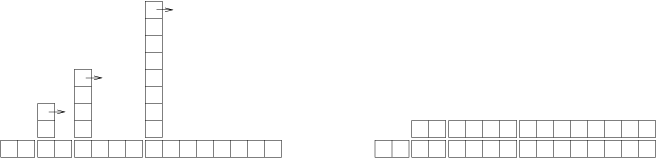
\includegraphics[width=5.5in]{../source/figs/towers.pdf}}
\caption{The cost of a hashtable add.\label{fig.hash}}
\end{figure}

The extra work of rehashing appears as a sequence of increasingly
tall towers with increasing space between them.  Now if you knock
over the towers, spreading the cost of resizing over all
adds, you can see graphically that the total cost after $n$
adds is $2n - 2$.

An important feature of this algorithm is that when we resize the
HashTable it grows geometrically; that is, we multiply the size by a
constant.  If you increase the size
arithmetically---adding a fixed number each time---the average time
per {\tt add} is linear.
\index{geometric resizing}

You can download my implementation of HashMap from
\url{http://thinkpython2.com/code/Map.py}, but remember that there
is no reason to use it; if you want a map, just use a Python dictionary.

\section{Glossary}

\begin{description}

\item[analysis of algorithms:] A way to compare algorithms in terms of
their run time and/or space requirements.
\index{analysis of algorithms}

\item[machine model:] A simplified representation of a computer used
to describe algorithms.
\index{machine model}

\item[worst case:] The input that makes a given algorithm run slowest (or
require the most space.
\index{worst case}

\item[leading term:] In a polynomial, the term with the highest exponent.
\index{leading term}

\item[crossover point:] The problem size where two algorithms require
the same run time or space.
\index{crossover point}

\item[order of growth:] A set of functions that all grow in a way
considered equivalent for purposes of analysis of algorithms.
For example, all functions that grow linearly belong to the same
order of growth.
\index{order of growth}

\item[Big-Oh notation:] Notation for representing an order of growth;
for example, $O(n)$ represents the set of functions that grow
linearly.
\index{Big-Oh notation}

\item[linear:] An algorithm whose run time is proportional to
problem size, at least for large problem sizes.
\index{linear}

\item[quadratic:] An algorithm whose run time is proportional to
$n^2$, where $n$ is a measure of problem size.
\index{quadratic}

\item[search:] The problem of locating an element of a collection
(like a list or dictionary) or determining that it is not present.
\index{search}

\item[hashtable:] A data structure that represents a collection of
key-value pairs and performs search in constant time.
\index{hashtable}

\end{description}


\printindex

\clearemptydoublepage
%\blankpage
%\blankpage
%\blankpage


\end{document}
